\documentclass{article}

  % packages
    % basic stuff for rendering math
    \usepackage[letterpaper, top=1in, bottom=1in, left=1in, right=1in]{geometry}
    \usepackage[utf8]{inputenc}
    \usepackage[english]{babel}
    \usepackage{amsmath} 
    \usepackage{amssymb}

    % extra math symbols and utilities
    \usepackage{mathtools}        % for extra stuff like \coloneqq
    \usepackage{mathrsfs}         % for extra stuff like \mathsrc{}
    \usepackage{centernot}        % for the centernot arrow 
    \usepackage{bm}               % for better boldsymbol/mathbf 
    \usepackage{enumitem}         % better control over enumerate, itemize
    \usepackage{hyperref}         % for hypertext linking
    \usepackage{fancyvrb}          % for better verbatim environments
    \usepackage{newverbs}         % for texttt{}
    \usepackage{xcolor}           % for colored text 
    \usepackage{listings}         % to include code
    \usepackage{lstautogobble}    % helper package for code
    \usepackage{parcolumns}       % for side by side columns for two column code
    \usepackage{algorithm}
    \usepackage{algpseudocode}
    \algblock{Class}{EndClass}

    % page layout
    \usepackage{fancyhdr}         % for headers and footers 
    \usepackage{lastpage}         % to include last page number in footer 
    \usepackage{parskip}          % for no indentation and space between paragraphs    
    \usepackage[T1]{fontenc}      % to include \textbackslash
    \usepackage{footnote}
    \usepackage{etoolbox}

    % for custom environments
    \usepackage{tcolorbox}        % for better colored boxes in custom environments
    \tcbuselibrary{breakable}     % to allow tcolorboxes to break across pages

    % figures
    \usepackage{pgfplots}
    \pgfplotsset{compat=1.18}
    \usepackage{float}            % for [H] figure placement
    \usepackage{tikz}
    \usepackage{tikz-cd}
    \usepackage{circuitikz}
    \usetikzlibrary{arrows, arrows.meta}
    \usetikzlibrary{positioning}
    \usetikzlibrary{calc}
    \usepackage{graphicx}
    \usepackage{caption} 
    \usepackage{subcaption}
    \captionsetup{font=small}

    % for tabular stuff 
    \usepackage{dcolumn}

    \usepackage[nottoc]{tocbibind}
    \pdfsuppresswarningpagegroup=1
    \hfuzz=5.002pt                % ignore overfull hbox badness warnings below this limit

  % New and replaced operators
    \DeclareMathOperator{\Tr}{Tr}
    \DeclareMathOperator{\Sym}{Sym}
    \DeclareMathOperator{\Span}{span}
    \DeclareMathOperator{\std}{std}
    \DeclareMathOperator{\Cov}{Cov}
    \DeclareMathOperator{\Var}{Var}
    \DeclareMathOperator{\Corr}{Corr}
    \DeclareMathOperator{\pos}{pos}
    \DeclareMathOperator*{\argmin}{\arg\!\min}
    \DeclareMathOperator*{\argmax}{\arg\!\max}
    \newcommand{\qed}{\hfill$\blacksquare$}     % I like QED squares to be black

  % Custom Environments
    \newtcolorbox[auto counter, number within=section]{question}[1][]
    {
      colframe = orange!25,
      colback  = orange!10,
      coltitle = orange!20!black,  
      breakable, 
      title = \textbf{Question \thetcbcounter ~(#1)}
    }

    \newtcolorbox[auto counter, number within=section]{exercise}[1][]
    {
      colframe = teal!25,
      colback  = teal!10,
      coltitle = teal!20!black,  
      breakable, 
      title = \textbf{Exercise \thetcbcounter ~(#1)}
    }
    \newtcolorbox[auto counter, number within=section]{solution}[1][]
    {
      colframe = violet!25,
      colback  = violet!10,
      coltitle = violet!20!black,  
      breakable, 
      title = \textbf{Solution \thetcbcounter}
    }
    \newtcolorbox[auto counter, number within=section]{lemma}[1][]
    {
      colframe = red!25,
      colback  = red!10,
      coltitle = red!20!black,  
      breakable, 
      title = \textbf{Lemma \thetcbcounter ~(#1)}
    }
    \newtcolorbox[auto counter, number within=section]{theorem}[1][]
    {
      colframe = red!25,
      colback  = red!10,
      coltitle = red!20!black,  
      breakable, 
      title = \textbf{Theorem \thetcbcounter ~(#1)}
    } 
    \newtcolorbox[auto counter, number within=section]{corollary}[1][]
    {
      colframe = red!25,
      colback  = red!10,
      coltitle = red!20!black,  
      breakable, 
      title = \textbf{Corollary \thetcbcounter ~(#1)}
    } 
    \newtcolorbox[auto counter, number within=section]{proof}[1][]
    {
      colframe = orange!25,
      colback  = orange!10,
      coltitle = orange!20!black,  
      breakable, 
      title = \textbf{Proof. }
    } 
    \newtcolorbox[auto counter, number within=section]{definition}[1][]
    {
      colframe = yellow!25,
      colback  = yellow!10,
      coltitle = yellow!20!black,  
      breakable, 
      title = \textbf{Definition \thetcbcounter ~(#1)}
    } 
    \newtcolorbox[auto counter, number within=section]{example}[1][]
    {
      colframe = blue!25,
      colback  = blue!10,
      coltitle = blue!20!black,  
      breakable, 
      title = \textbf{Example \thetcbcounter ~(#1)}
    } 
    \newtcolorbox[auto counter, number within=section]{code}[1][]
    {
      colframe = green!25,
      colback  = green!10,
      coltitle = green!20!black,  
      breakable, 
      title = \textbf{Code \thetcbcounter ~(#1)}
    } 
    \newtcolorbox[auto counter, number within=section]{algo}[1][]
    {
      colframe = green!25,
      colback  = green!10,
      coltitle = green!20!black,  
      breakable, 
      title = \textbf{Algorithm \thetcbcounter ~(#1)}
    } 
    \definecolor{cverbbg}{gray}{0.93}
    \newenvironment{cverbatim}
      {\SaveVerbatim{cverb}}
      {\endSaveVerbatim
        \flushleft\fboxrule=0pt\fboxsep=.5em
        \colorbox{cverbbg}{%
          \makebox[\dimexpr\linewidth-2\fboxsep][l]{\BUseVerbatim{cverb}}%
        }
        \endflushleft
    }

    \definecolor{dkgreen}{rgb}{0,0.6,0}
    \definecolor{gray}{rgb}{0.5,0.5,0.5}
    \definecolor{mauve}{rgb}{0.58,0,0.82}
    \definecolor{lightgray}{gray}{0.93}
    \renewcommand{\algorithmiccomment}[1]{\hfill$\triangleright$\textcolor{blue}{#1}}

    % default options for listings (for code)
    \lstset{
      autogobble,
      frame=ltbr,
      language=Python,                           % the language of the code
      aboveskip=3mm,
      belowskip=3mm,
      showstringspaces=false,
      columns=fullflexible,
      keepspaces=true,
      basicstyle={\small\ttfamily},
      numbers=left,
      firstnumber=1,                        % start line number at 1
      numberstyle=\tiny\color{gray},
      keywordstyle=\color{blue},
      commentstyle=\color{dkgreen},
      stringstyle=\color{mauve},
      backgroundcolor=\color{lightgray}, 
      breaklines=true,                      % break lines
      breakatwhitespace=true,
      tabsize=3, 
      xleftmargin=2em, 
      framexleftmargin=1.5em, 
      stepnumber=1
    }

  % Page style
    \pagestyle{fancy}
    \fancyhead[L]{Deep Learning}
    \fancyhead[C]{Muchang Bahng}
    \fancyhead[R]{Summer 2023, Spring 2025} 
    \fancyfoot[C]{\thepage / \pageref{LastPage}}
    \renewcommand{\footrulewidth}{0.4pt}          % the footer line should be 0.4pt wide
    \renewcommand{\thispagestyle}[1]{}  % needed to include headers in title page
    \renewcommand{\thefootnote}{\arabic{footnote}}

\begin{document}

\title{Deep Learning}
\author{Muchang Bahng}
\date{Summer 2023, Spring 2025}

\maketitle
\tableofcontents
\pagebreak 


This covers computability theory, complexity theory, and automata theory. 
Alphabet. Boolean logic


\section{Multi-Layered Perceptrons} 

  Why do we even \textit{need} deep neural networks in the first place? Well with classical machine learning, the models that we worked with were ``simple' enough\footnote{I am using simple in a very loose sense, since this doesn't really mean that the model space is finite-dimensional or have any correlation with complexity.} to interpret. For example, linear regression had a simple parametric form, and decision trees, though nonlinear and nonparametric, were very interpretable both in training and prediction. However, it may be that the very notion of interpretability is limiting the power of our models. Maybe the world is so complex that it may not be even possible to model it with these interpretable functions. Therefore, we should try to create a model with a simple enough parametrization, but something that is expressive enough to cover an extremely large space of functions. This may sound contradictory, but it is possible. We build upon what we already know: generalized linear models. 

  In simple regression, we transform the inputs into the relevant features $\mathbf{x}_n \mapsto \boldsymbol{\phi} (\mathbf{x}_n) = \boldsymbol{\phi}_n$ and then, when we construct a generalized linear model, we assume that the conditional distribution $Y \mid X = x$ is in the canonical exponential family, with some natural parameter $\eta(x)$ and expected mean $\mu(x) = \mathbb{E}[Y \mid X = x]$. Then, to choose the link function $g$ that related $g(\mu(x)) = x^T \beta$, we can set it to be the canonical link $g$ that maps $\mu$ to $\eta$. That is, we have $g(\mu(x)) = x^T \beta = \eta (x)$ such that the natural parameter is linearly dependent on the input. The inverse $g^{-1}$ of the link function is called the \textbf{activation function}, which connects the expected mean to a linear function of $x$. 
  \begin{equation}
    h_\beta (x) = g^{-1} (x^T \beta) = \mu(x) = \mathbb{E}[Y \mid X = x]
  \end{equation}
  Now, note that for a classification problem, the decision boundary defined in the $\boldsymbol{\phi}$ feature space is linear, but it may not be linear in the input space $\mathcal{X}$. 

  \begin{figure}[H]
    \centering
    \begin{subfigure}[t]{0.24\textwidth}
      \centering
      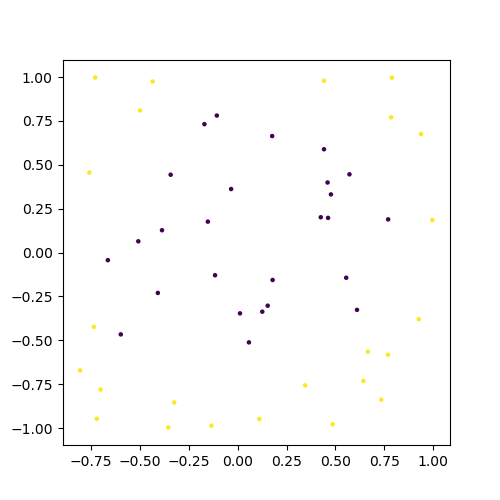
\includegraphics[width=\textwidth]{img/01_MLP/untrans_data.png}
      \caption{Data in space $\mathcal{X} = \mathbb{R}^2$.}
      \label{fig:raw_points}
    \end{subfigure}
    \hfill
    \begin{subfigure}[t]{0.24\textwidth}
      \centering
      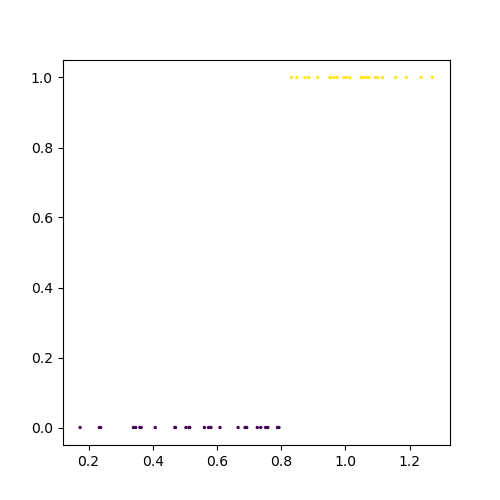
\includegraphics[width=\textwidth]{img/01_MLP/trans_data.png}
      \caption{Transformed data $\phi(\mathbf{x}) = \|\mathbf{x}\|$.}
      \label{fig:transformed_points}
    \end{subfigure}
    \hfill
    \begin{subfigure}[t]{0.24\textwidth}
      \centering
      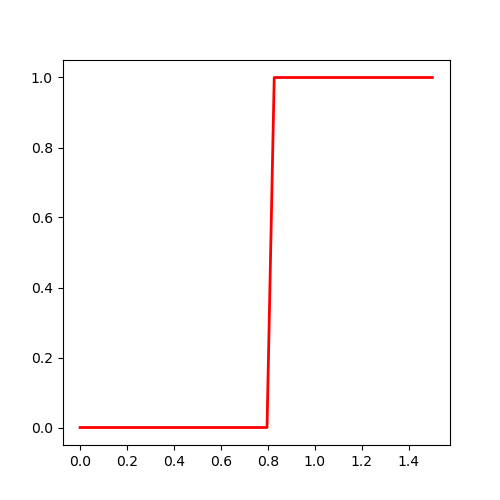
\includegraphics[width=\textwidth]{img/01_MLP/trans_fit.png}
      \caption{Logistic fit in transformed space.}
      \label{fig:transformed_trained}
    \end{subfigure}
    \hfill
    \begin{subfigure}[t]{0.24\textwidth}
      \centering
      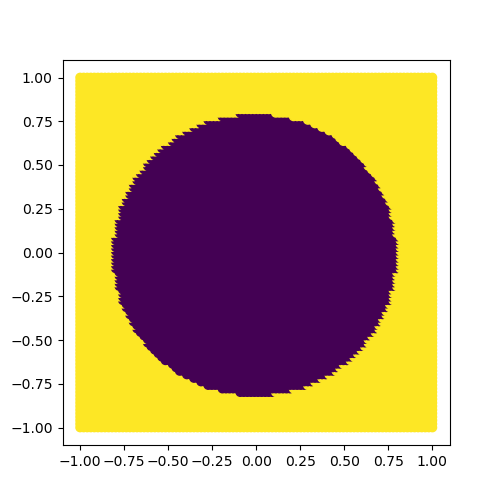
\includegraphics[width=\textwidth]{img/01_MLP/untrans_fit.png}
      \caption{Logistic fit to data in input space.}
      \label{fig:raw_trained}
    \end{subfigure}
    \caption{Consider the set of points in $\mathbb{R}^2$ with the corresponding class. We transform the features to $\boldsymbol{\phi}(x_1, x_2) = x_1^2 + x_2^2$, which gives us a new space to work with. Fitting logistic regression onto this gives a linear decision boundary in the space $\boldsymbol{\phi}$, but the boundary is circular in $\mathcal{X} = \mathbb{R}^2$.}
    \label{fig:logistic_transformed}
  \end{figure}

  We would like to extend this model by making the basis functions $\boldsymbol{\phi}_n$ depend on the parameters $\mathbf{w}$ and then allow these parameters to be adjusted during training. 

\subsection{Feedforward Fully-Connected Networks}

  So how should we construct parametric nonlinear basis functions? One way is to have a similar architecture as GLMs by having a linear map followed by an activation function $f(x) = \sigma(w^T x + b)$. The simplest such function with the activation function as the step function 
  \begin{equation}
    f(z) = \begin{cases} 1 & \text{ if } z \geq 0 \\ 0 & \text{ if } z < 0 \end{cases}
  \end{equation}
  is the perceptron algorithm. It divides $\mathbb{R}^d$ using a hyperplane $\boldsymbol{\omega}^T \mathbf{x} + b = 0$ and linearly classifies all points on one side to value $1$ and the other side to value $0$. This is similar to a neuron, which takes in a value and outputs a ``signal" if the function evaluated gets past a threshold. However, for reasons regarding training these networks, we would like to use smooth activation functions for this, so we would use different activations. Hence we have a neuron. 

  \begin{definition}[Neuron]
    A \textbf{neuron} is a function of form 
    \begin{equation}
      y = \sigma(\mathbf{w}^T x  + b)
    \end{equation}
    where $\sigma: \mathbb{R} \rightarrow \mathbb{R}$ is any nonlinear function, called an \textbf{activation functions}. 
  \end{definition}
  
  Ultimately, a neural net is really just a generalized linear model with some trained feature extractors, which is why in practice, if researchers want to predict a smaller dataset, they take a pretrained model on a related larger dataset and simply tune the final layer, since the second last layer most likely encodes all the relevant features. This is called \textit{transfer learning}. But historically, it was called a \textit{multilayer perceptron} and the name stuck. 

  \begin{definition}[Feedforward, Fully-Connected Multilayer Perceptron]
    A $L$-layer \textbf{multilayer perceptron (MLP)} $f_\theta : \mathbb{R}^D \rightarrow \mathbb{R}^M$, with parameters $\theta$, is a function of form 
    \begin{equation}
      h_\theta (\mathbf{x}) \coloneqq \sigma^{[L]} \circ W^{[L]} \circ \sigma^{[L-1]} \circ W^{[L-1]} \circ \cdots \circ \sigma^{[1]} \circ W^{[1]} (\mathbf{x})
    \end{equation}
    where $\sigma^{[l]}: \mathbb{R}^{N^{[l]}} \rightarrow \mathbb{R}^{N^{[l]}}$ is an activation function and $W^{[l]}: \mathbb{R}^{N^{[l-1]}} \rightarrow \mathbb{R}^{N^{[l]}}$ is an affine map. We will use the following notation. 
    \begin{enumerate}
      \item The inputs will be labeled $\mathbf{x} = a^{[0]}$ which is in $\mathbb{R}^{N^{[0]}} = \mathbb{R}^D$. 
      
      \item We map $a^{[l]} \in \mathbb{R}^{N^{[l]}} \mapsto W^{[l+1]} a^{[l]} + b^{[l+1]}= z^{[l+1]} \in \mathbb{R}^{N^{[l+1]}}$, where $z$ denotes a vector after an affine transformation. 
      \item We map $z^{[l+1]} \in \mathbb{R}^{N^{[l+1]}} \mapsto \sigma(z^{[l+1]}) = a^{[l+1]} \in \mathbb{R}^{N^{[l+1]}}$, where $a$ denotes a vector after an activation function. 
      \item We keep doing this until we reach the second last layer with vector $a^{[L-1]}$. 
      \item Now we want our last layer to be our predicted output. Based on our assumptions of the problem, we construct a generalized linear model with some inverse link function $g$. We perform one more affine transformation $a^{[L-1]} \mapsto W^{[L]} a^{[L-1]} + b^{[L]} = z^{[L]}$, followed by the link function to get our prediction: $a^{[L]} = g(z^{[L]}) = h_{\theta} (\mathbf{x}) \in \mathbb{R}^M$. 
    \end{enumerate}

    \begin{figure}[H]
      \centering 
      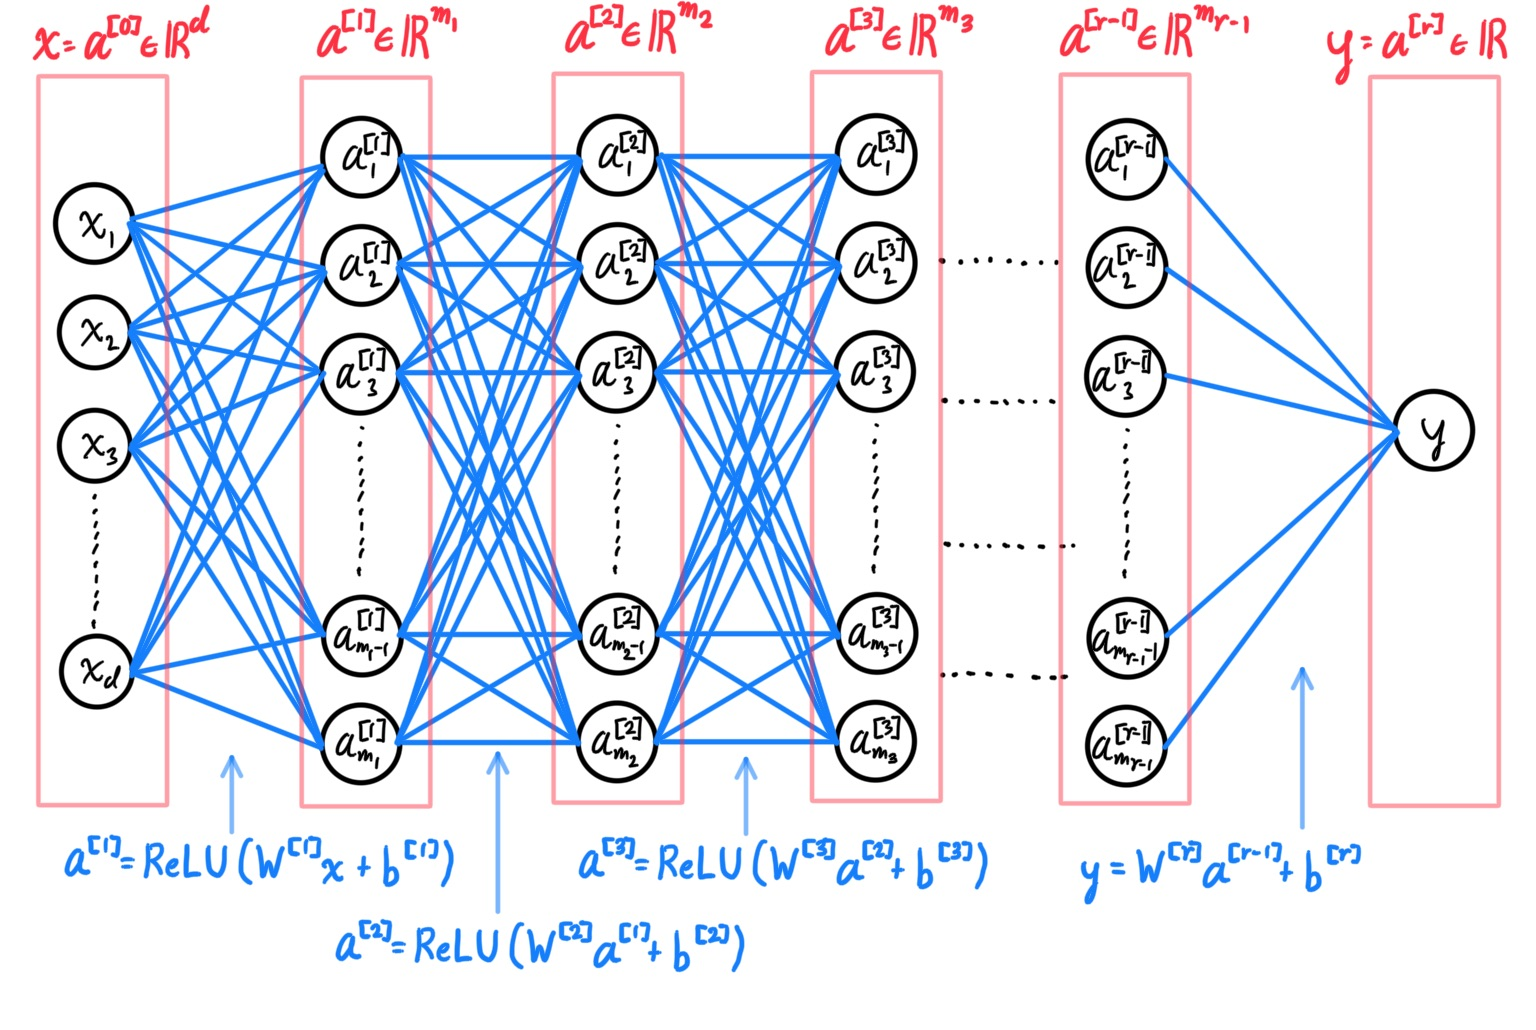
\includegraphics[scale=0.17]{img/01_MLP/Multilayer_Neural_Net.jpg}
      \caption{If there does not exist any edge from a potential input $x$ to an output $y$, then this means that $x$ is not relevant in calculating $y$. However, we usually work with \textbf{fully-connected neural networks}, which means that every input is relevant to calculating every output, since we usually cannot make assumptions about which variables are relevant or not. We can stack multiple neurons such that one neuron passes its output as input into the next neuron, resulting in a more complex function. } 
      \label{fig:multilayer_neural_net}
    \end{figure}
  \end{definition}

  Note that each layer corresponds to how close a neuron is to the output. But really any neuron can be a function of any other neuron. For example, we can connect a neuron from layer $4$ back to a neuron of layer $1$. For now, we will consider networks that are restricted to a \textbf{feed-forward} architecture, in other words having no closed directed cycles. 

  \begin{code}[Parameters and Neural Nets in PyTorch] 
    At this point, you have learned the theory of MLPs. To actually implement them in PyTorch, look at this module \href{code/01_MLP/parameters.ipynb}{here}, which will tell you on how to construct linear maps and activations functions, and more importantly see how you can look at the weights, modify them, and see how they are initialized. You can then learn how to explore the weights and biases of a neural network. 
  \end{code}

\subsection{Function Space and Universal Approximation} 

  Great, so we have defined our architecture, but how do we know that this class of functions is expressive? Neural networks have been mathematically studied back in the 1980s, and the reason that they are so powerful is that we can theoretically prove the limits on what they can learn. For very specific classes of functions, the results are easier, but for more general ones, it becomes much harder. We prove one of the theorems below. 

  Let us think about how one would construct approximations for such functions. Like in measure theory, we can think of every measurable function as a linear combination of a set of bump functions, and so we can get a neural network to do the same.

  \begin{example}[Bump Functions in $\mathbb{R}$] 
    Assuming the sigmoid activation function is used, the bump function 
    \begin{equation}
      f(x) = \begin{cases} 1 & \text{ if } a < x < b \\ 0 & \text{ if else} \end{cases}
    \end{equation}
    can be approximated by taking a linear combination of a sigmoid function stepping up and one stepping down. That is, 
    \begin{equation}
      f(x) \approx \frac{1}{2} \sigma \big( k( x - a)\big) - \frac{1}{2} \sigma \big( k (x - b) \big)
    \end{equation}
    where $k$ is a scaling constant that determines how steep the steps are for each function. Therefore, as $k \rightarrow \infty$, the function begins to look more like a step function. 
    \begin{figure}[H]
      \centering 
      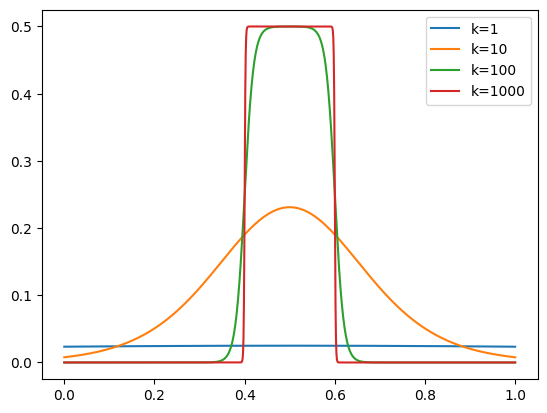
\includegraphics[scale=0.6]{img/01_MLP/bump_functions_1d.png}
      \caption{Bump function approximated with $a = 0.4, b = 0.6$, with differing values of $k$. } 
      \label{fig:bump_functions_1d}
    \end{figure}
  \end{example}

  \begin{example}[Bump Functions in $\mathbb{R}^2$]
    To do this for a 2-D step function, of the form 
    \begin{equation}
      f(x_1, x_2) = \begin{cases} 1 \text{ if } a < x_1 < b \\ 0 & \text{ if else} \end{cases}
    \end{equation}
    this is a simple extension of the first one. We just don't need to make our linear combination dependent on $x_2$ and we're done.
    \begin{equation}
      f(x) \approx \frac{1}{2} \sigma \big( k( x_1 - a)\big) - \frac{1}{2} \sigma \big( k (x_1 - b) \big)
    \end{equation}
  \end{example} 

  \begin{example}[Tower Functions in $\mathbb{R}^2$] 
    Now to construct a tower function of the form 
    \begin{equation}
      f(x_1, x_2) = \begin{cases} 1 & \text{ if } a_1 < x_1 < b_1, a_2 < x_2 < b_2 \\ 0 & \text{ if else} \end{cases}
    \end{equation}
    we need slightly more creativity. Now we can approximate it by doing 
    \begin{equation}
      f(x) \approx \sigma \bigg( k_2 \big[ \sigma\big( k_1 (x_1 - a_1)\big) - \sigma\big( k_1 (x_1 -b_1)\big) + \sigma \big( k_1 (x_2 - a_2)\big) - \sigma\big(k_1 (x_2 - b_2)\big)  big] - b_2\bigg)
    \end{equation}
  \end{example} 

  At this point, we can see how this would extend to $\mathbb{R}^n$, and by isolating parts of the network we can have it approximate tower functions that are completely separate from each other, at any height, and then finally take a linear combination of them to approximate the original function of interest.  

  \begin{theorem}[CS671 Fall 2023 PS5]
    Suppose you have a 2D, $L$-lipschitz function $f(x_1, x_2)$ defined on a unit square ($x_1, x_2 \in \left [0,1 \right ]$). You want to approximate this with an arbitrary neural net $\Tilde{f}$ such that
    \begin{equation}
      \sup_{x \in [0, 1]^2} |f(x) - \Tilde{f}(x)| \leq \epsilon
    \end{equation}
    If we divide the square into a checkerboard of $K \times K$ nonoverlapping squares, approximate the restriction of $f$ to each subsquare with a tower function, what is the least $K$ we would need to ensure that the error is less than $\epsilon$? 
  \end{theorem} 

  Early in the development of the theory of neural nets, An Mei Chen, (currently VP of engineering in Qualcomm) showed that for certain neural networks, there are multiple parameters $\theta$ that map to the same function $f$. \cite{symmetry}

  \begin{theorem}[Parameter Symmetry]
    Consider a 2-layer feedforward network of form 
    \begin{equation}
      f = W^{[2]} \circ \sigma \circ W^{[1]}
    \end{equation} 
    where $\sigma = \tanh$. Let $z$ be the hidden vector. We can see that by changing the signs of the $i$th row of $W^{[1]}$, $z_i$'s sign will be flipped. From the properties that $\tanh$ is an odd function (i.e. $\tanh(-x) = - \tanh(x)$), therefore the activation will be also sign-flipped, but this effect can be negated by flipping the $i$th column of the $W^{[2]}$. Therefore, given that $z \in R^{N}$, i.e there are $N$ hidden units, we can choose any set of row-column pairs of the weight matrices to invert, leading to a total of $2^N$ different weightings that produce the same function $f$. 

    Similarly, imagine that we permute the columns of $W^{[2]}$ and rows of $W^{[1]}$ in the same way. Then this will also lead to an invariance in $f$, and so this leads to $N! 2^N$ different weight vectors that lead to the same function! 
  \end{theorem}

\subsection{Tensors} 

  In numerical computing packages like \texttt{numpy} in Python and \texttt{eigen} in C++, we often work with scalars, vectors, and matrices. From linear algebra, the generalization of these objects is a tensor, which is an element of a tensor product space.\footnote{For a refresher, look at my linear algebra notes.} The full mathematical abstraction is rarely needed in practice, and so developers call tensors by their realization as \textit{multidimensional arrays}. 
  
  \begin{definition}[Tensor]
    A \textbf{tensor} is an element of a tensor product space $\bigotimes_i V_i$. It is represented as a \textbf{multidimensional array} of shape $(\dim(V_1), \ldots, \dim(V_n))$. 
  \end{definition}

  If we were trying to build a \texttt{Tensor} class from scratch, what attributes should it have? Well obviously we need the actual data in the tensor, which we will call \texttt{storage}, plus some metadata about the \texttt{shape} (in math, known as the tensor \textit{rank}). Usually, these packages optimize as much as possible for efficiency, and so these are implemented as C-style arrays, which then requires knowledge of the type of each element of the Tensor, called the \texttt{dtype}. Great, with these three attributes, we can do almost every type of arithmetic manipulation. Let's first introduce the most basic math tensor operations, which includes the normal operations supported in an algebra, plus some other ones. We will denote the shapes as well. 
  \begin{enumerate}
    \item \textit{Tensor Addition}. 
    \item \textit{Tensor Additive Inverse}. 
    \item \textit{Scalar Multiplication}. 
    \item \textit{Matrix Multiplication}. 
    \item \textit{Elementwise Multiplication}. 
    \item \textit{Elementwise Multiplicative Inverse}.  
    \item \textit{Transpose}. 
  \end{enumerate} 

  We would probably like some constructors that allows you to directly initialize tensors filled with $0$s (\texttt{zeros}), $1$s (\texttt{ones}), a multiplicative identity (\texttt{eye}\footnote{homophone for $I$, used to denoted the identity matrix.}) Some random initializers would be good, such as sampling from uniforms (\texttt{uniform}), \texttt{gaussians} (\texttt{gaussian}, \texttt{randn}). 

  Finally, we would like some very fundamental operations, such as typecasting, comparison, and indexing as well. 

  \begin{algorithm}[H]
    \caption{Tensor Class Implementation}
    \begin{algorithmic}[1]
    \State \textbf{class} Tensor:
        \State \textbf{Attributes:}
        \State \hspace{1em}storage: array  \Comment{Underlying data storage}
        \State \hspace{1em}shape: tuple    \Comment{Dimensions of tensor}
        \State \hspace{1em}dtype: type     \Comment{Data type of elements}

        \State \textbf{Constructors:}
        \State \texttt{def \_\_init\_\_(data, shape, dtype):}
            \State \hspace{2em}Initialize tensor with given data, shape, and dtype

        \State \textbf{Static Constructors:}
        \State \texttt{@staticmethod}
        \State \texttt{def zeros(shape, dtype):}
            \State \hspace{2em}\Return tensor filled with zeros
        \State \texttt{@staticmethod}
        \State \texttt{def ones(shape, dtype):}
            \State \hspace{2em}\Return tensor filled with ones
        \State \texttt{@staticmethod}
        \State \texttt{def eye(n, dtype):}
            \State \hspace{2em}\Return n×n identity matrix
        \State \texttt{@staticmethod}
        \State \texttt{def uniform(shape, low, high, dtype):}
            \State \hspace{2em}\Return tensor with uniform random values
        \State \texttt{@staticmethod}
        \State \texttt{def gaussian(shape, mean, std, dtype):}
            \State \hspace{2em}\Return tensor with gaussian random values

        \State \textbf{Arithmetic Operations:}
        \State \texttt{def \_\_add\_\_(self, other):}
            \State \hspace{2em}\Return element-wise addition
        \State \texttt{def \_\_neg\_\_(self):}
            \State \hspace{2em}\Return additive inverse
        \State \texttt{def \_\_mul\_\_(self, other):}
            \State \hspace{2em}\Return scalar or element-wise multiplication
        \State \texttt{def matmul(self, other):}
            \State \hspace{2em}\Return matrix multiplication
        \State \texttt{def \_\_truediv\_\_(self, other):}
            \State \hspace{2em}\Return element-wise division
        \State \texttt{def transpose(self):}
            \State \hspace{2em}\Return transposed tensor

        \State \textbf{Utility Operations:}
        \State \texttt{def \_\_repr\_\_(self):}
            \State \hspace{2em}\Return string representation
        \State \texttt{def \_\_str\_\_(self):}
            \State \hspace{2em}\Return human-readable string
        \State \texttt{def \_\_getitem\_\_(self, index):}
            \State \hspace{2em}\Return indexed value(s)
        \State \texttt{def \_\_eq\_\_(self, other):}
            \State \hspace{2em}\Return element-wise equality comparison
    \end{algorithmic}
  \end{algorithm}

  Note that there are other operations, such as concatenation, splitting, and stacking that would be a good idea to implement.  

  \subsubsection{Strides} 

    A specific property of PyTorch is that they use strides as another source of metadata in storing tensors, which greatly speeds up operations. Consider that we want to transpose the first two dimensions of a tensor. Then, we would have to create a new tensor and fill it in with all the elements, which may be too computationally expensive for such a small operation. 

    \begin{definition}[Stride] 
      Given a tensor $T$ of size $(N_1, \ldots N_M)$, it is stored as a contiguous array of $\prod_m T_m$ elements, and we can index it as 
      \begin{equation}
        T[n_1, n_2, \ldots, n_M], \;\;\; 1 \leq n_i \leq N_i
      \end{equation} 
      To counteract this, the \textbf{stride} is a array $S$ of $M$ elements, 
      \begin{equation}
        S = (S_1, \ldots, S_M)
      \end{equation} 
      where indexing with some $I = (n_1, \ldots, n_M)$ is equivalent to computing $S \cdot I$ and taking that index in the array in memory. It defines a mapping. 
    \end{definition}

    If we do some calculation, the default stride of such a vector is defined 
    \begin{equation}
      S_m = \prod_{m < j} N_j, \;\;\; S_M = 1
    \end{equation}

    \begin{example}[Transposing]
      If we want to transpose the tensor above, then we change the stride from 
      \begin{equation}
        S = \bigg( \prod_{1 < j} N_j , \prod_{2 < j} N_j, \ldots, 1 \bigg)
      \end{equation} 
      to 
      \begin{equation}
        S = \bigg( \prod_{2 < j} N_j , \prod_{1 < j} N_j, \ldots, 1 \bigg)
      \end{equation} 
    \end{example}

  \subsubsection{Automatic Differentiation} 

    \begin{lemma}[Derivative of $+/-$]
      Given two tensors $X, Y$ and $Z_+ = X + Y, Z_{-} = X - Y$, we have 
      \begin{align}
        \frac{\partial Z_+}{\partial X} = +1 && \frac{\partial Z_+}{\partial Y} = +1 \\ 
        \frac{\partial Z_-}{\partial X} = +1 && \frac{\partial Z_-}{\partial Y} = -1 
      \end{align}
      where $\pm1$ are tensors of $1$ or $-1$s of the same shape as $X, Y$. 
    \end{lemma}

    \begin{lemma}[Derivative of Element-wise Multiplication]
      Given two tensors $X, Y$ and $Z = X \odot Y$, we have 
      \begin{align}
        \frac{\partial Z}{\partial X} = Y && \frac{\partial Z}{\partial Y} = X
      \end{align}
    \end{lemma} 

    \begin{lemma}[Derivative of Matrix Multiplication]
      Given $X \in (N, M)$ and $Y \in (M, P)$, with $Z = XY \in (N, P)$, the derivative of matrix multiplication is 
      \begin{align}
        \frac{\partial Z}{\partial X} \in (N, P, N, M) && \bigg( \frac{\partial Z}{\partial X} \bigg)_{i, j, k, l} \coloneqq \frac{\partial Z_{i, j}}{\partial X_{k, l}} \\
        \frac{\partial Z}{\partial Y} \in (N, P, M, P) && \bigg( \frac{\partial Z}{\partial Y} \bigg)_{i, j, k, l} \coloneqq \frac{\partial Z_{i, j}}{\partial Y_{k, l}} 
      \end{align} 
    \end{lemma} 

\subsection{Forward and Back Propagation}

  Back in the supervised learning notes, we have gone through the derivation for linear, logistic, and softmax regression. It turns out that despite them having very different architectures, with a identity, sigmoid, and softmax activation function, our choice of loss to be the mean squared loss, the binary cross-entropy, and the cross-entropy loss, had given very cute formulas in computing the gradient of the loss. Unfortunately, the formulas do not get cute when we differentiate neural networks, but they do come in a very structured way. To gain intuition, I would recommend to go over the exercises at the end of the chapter labeled ECE 689 Fall 2021 Midterm. If you just use chain rule to do the calculations, you can see that they require us to compute all the intermediate $z^{(i)}$'s and the $a^{(i)}$'s, a process called \textit{forward propagation}, before we compute the gradients. 

  \begin{definition}[Forward Propagation]
    Given an MLP $f$ and an input $x$, the process of sequentially evaluating 
    \begin{equation}
      x = a^{[0]} \mapsto z^{[1]} \mapsto a^{[1]} \mapsto \ldots \mapsto z^{[L]} \mapsto a^{[L]} = f(x)
    \end{equation}
    is called \textbf{forward propagation}. 
  \end{definition} 

  When we want to compute the derivative of $f$. we can see that the intermediate partial derivatives in the chain rule are repeatedly used. That is, if we have layer $0 \leq l \leq L$, then to compute the derivative with respect to the $l$th layer we use the chain rule 
  \begin{equation}
    \frac{\partial f}{\partial z^{[l]}} = \frac{\partial f}{\partial z^{[l+1]}} \cdot \frac{z^{[l+1]}}{z^{[l]}}
  \end{equation}
  which requires us to know the derivative at the $(l+1)$th layer, along with the current values of $z^{[l]}, z^{[l+1]}$ to evaluate the derivatives at the current point. Therefore, we must complete forward propagation first and then compute \textit{backwards} from the result to the input to compute the gradients. 

  \begin{definition}[Backward Propagation]
    Given an MLP $f$ with input $x$ that has been forward propagated, the process of sequentially evaluating 
    \begin{equation}
      \frac{\partial f}{\partial a^{[L]}} \mapsto \frac{\partial f}{\partial z^{[L]}} \mapsto \ldots \mapsto \frac{\partial f}{\partial z^{[L]}}, 
    \end{equation}
    is called \textbf{backward propagation}, or \textbf{backprop}. 
  \end{definition}

  Backpropagation is not hard, but it is cumbersome notation-wise. What we really want to do is just compute a very long vector with all of its partials $\partial E / \partial \boldsymbol{\theta}$. 

  \begin{algo}[Backpropagation]
    To compute $\frac{\partial E_n}{\partial w_{ji}^{[l]}}$, it would be natural to split it up into a portion where $E_n$ is affected by the term before activation $\mathbf{z}^{[l]}$ and how that is affected by $w_{ji}^{[l]}$. The same goes for the bias terms. 
    \begin{equation}
      \frac{\partial E_n}{\partial w_{ji}^{[l]}} = \underbrace{\frac{\partial E_n}{\partial \mathbf{z}^{[l]}}}_{1 \times N^{[l]}} \cdot \underbrace{\frac{\partial \mathbf{z}^{[l]}}{\partial w_{ji}^{[l]}}}_{N^{[l]} \times 1} \text{ and } \frac{\partial E_n}{\partial b_{i}^{[l]}} = \underbrace{\frac{\partial E_n}{\partial \mathbf{z}^{[l]}}}_{1 \times N^{[l]}} \cdot \underbrace{\frac{\partial \mathbf{z}^{[l]}}{\partial b_{i}^{[l]}}}_{N^{[l]} \times 1}
    \end{equation}
    It helps to visualize that we are focusing on 
    \begin{equation}
      \mathbf{h}_{\boldsymbol{\theta}} (\mathbf{x}) = g\big( \ldots \sigma( \underbrace{\mathbf{W}^{[l]} \mathbf{a}^{[l-1]} + \mathbf{b}^{[l]}}_{\mathbf{z}^{[l]}} )  \ldots \big)
    \end{equation}
    We can expand $\mathbf{z}^{[l]}$ to get 
    \begin{equation}
      \mathbf{z}^{[l]} = \begin{pmatrix} w_{11}^{[l]} & \ldots & w_{1 N^{[l-1]}}^{[l]} \\ \vdots & \ddots & \vdots \\ w_{N^{[l]} 1}^{[l]} & \ldots & w_{N^{[l]} N^{[l-1]}}^{[l]} \end{pmatrix} 
      \begin{pmatrix} a^{[l-1]}_1 \\ \vdots \\ a^{[l-1]}_{N^{[l-1]}} \end{pmatrix} + \begin{pmatrix} b_1^{[l]} \\ \vdots \\ b_{N^{[l]}_{[l]}} \end{pmatrix}
    \end{equation}
    $w_{ji}^{[l]}$ will only show up in the $j$th term of $\mathbf{z}^{[l]}$, and so the rest of the terms in $\frac{\partial \mathbf{z}^{[l]}}{\partial w_{ji}^{[l]}}$ will vanish. The same logic applies to $\frac{\partial \mathbf{z}^{[l]}}{\partial b_{i}^{[l]}}$, and so we really just have to compute 
    \begin{equation}
      \frac{\partial E_n}{\partial w_{ji}^{[l]}} = \underbrace{\frac{\partial E_n}{\partial z^{[l]}_j}}_{1 \times 1} \cdot \underbrace{\frac{\partial z^{[l]}_j}{\partial w_{ji}^{[l]}}}_{1 \times 1} = \delta^{[l]}_j \cdot \frac{\partial z^{[l]}_j}{\partial w_{ji}^{[l]}} \text{ and } \frac{\partial E_n}{\partial b_{i}^{[l]}} = \underbrace{\frac{\partial E_n}{\partial z^{[l]}_j}}_{1 \times 1} \cdot \underbrace{\frac{\partial z^{[l]}_j}{\partial b_{i}^{[l]}}}_{1 \times 1} = \delta^{[l]}_j \cdot \frac{\partial z^{[l]}_j}{\partial b_{i}^{[l]}}
    \end{equation}
    where the $\delta_j^{[l]}$ is called the $j$th \textbf{error term} of layer $l$. If we look at the evaluated $j$th row, 
    \begin{equation}
      z_j^{[l]} = w_{j1}^{[l]} a_1^{[l-1]} + \ldots w_{j N^{[l-1]}} a^{[l-1]}_{N^{[l-1]}} + b_j^{[l]}
    \end{equation}
    We can clearly see that $\frac{\partial z^{[l]}_j}{\partial w_{ji}^{[l]}} = a_i^{[l-1]}$ and $\frac{\partial z^{[l]}_j}{\partial b_{i}^{[l]}} = 1$, which means that our derivatives are now reduced to 
    \begin{equation}
      \frac{\partial E_n}{\partial w_{ji}^{[l]}} = \delta_j^{[l]} a_i^{[l-1]}, \;\;\;\;\; \frac{\partial E_n}{\partial b_{i}^{[l]}} = \delta_j^{[l]}
    \end{equation}
    What this means is that we must know the intermediate values $\mathbf{a}^{[l-1]}$ beforehand, which is possible since we would compute them using forward propagation and store them in memory. Now note that the partial derivatives at this point have been calculated without any consideration of a particular error function or activation function. To calculate $\boldsymbol{\delta}^{[L]}$, we can simply use the chain rule to get 
    \begin{equation}
      \delta_j^{[L]} = \frac{\partial E_n}{\partial z_j^{[L]}} = \frac{\partial E_n}{\partial \mathbf{a}^{[L]}} \cdot \frac{\partial \mathbf{a}^{[L]}}{\partial z_j^{[L]}} = \sum_k \frac{\partial E_n}{\partial a_k^{[L]}} \cdot \frac{\partial a_k^{[L]}}{\partial z_j^{[L]}}
    \end{equation}
    which can be rewritten in the matrix notation
    \begin{equation}
      \boldsymbol{\delta}^{[L]} = \bigg( \frac{\partial \mathbf{g}}{\partial \mathbf{z}^{[L]}} \bigg)^T \bigg( \frac{\partial E_n}{\partial \mathbf{a}^{[L]}} \bigg) = \underbrace{\begin{bmatrix} \frac{\partial g_1}{\partial z_1^{[L]}} & \ldots & \frac{\partial g_{N^{[L]}}}{\partial z^{[L]}_1} \\ \vdots & \ddots & \vdots \\ \frac{\partial g_1}{\partial z^{[L]}_{N^{[L]}}} & \ldots & \frac{\partial g_{N^{[L]}}}{\partial z^{[L]}_{N^{[L]}}} \end{bmatrix}}_{N^{[L]} \times N^{[L]}} \begin{bmatrix} \frac{\partial E_n}{\partial a_1^{[L]}} \\ \vdots \\ \frac{\partial E_n}{\partial a_{N^{[L]}}^{[L]}} \end{bmatrix}
    \end{equation}
    Note that as soon as we make a model assumption on the form of the conditional distribution $Y \mid X = x$ (e.g. it is Gaussian), with it being in the exponential family, we immediately get two things: the loss function $E_n$ (e.g. sum of squares loss), and the canonical link function $\mathbf{g}$
    \begin{enumerate}
      \item If we assume that $Y \mid X = x$ is Gaussian in a regression (of scalar output) setting, then our canonical link would be $g(x) = x$, which gives the sum of squares loss function. Note that since the output is a real-valued scalar, $\mathbf{a}^{[L]}$ will be a scalar (i.e. the final layer is one node, $N^{[L]} = 1$). 
      \begin{equation}
        E_n = \frac{1}{2} (y^{(n)} - a^{[L]} )^2
      \end{equation}
      To calculate $\boldsymbol{\delta}^{[L]}$, we can simply use the chain rule to get 
      \begin{equation}
        \delta^{[L]} = \frac{\partial E_n}{\partial z^{[L]}} = \frac{\partial E_n}{\partial a^{[L]}} \cdot \frac{\partial a^{[L]}}{\partial z^{[L]}} = a^{[L]} - y^{(n)}
      \end{equation}

      \item For classification (of $M$ classes), we would use the softmax activation function (with its derivative next to it for convenience) 
      \begin{equation}
        \mathbf{g}(\mathbf{z}) = \mathbf{g} \bigg( \begin{bmatrix} z_1 \\ \vdots \\ z_M \end{bmatrix} \bigg) = \begin{bmatrix} e^{z_1} / \sum_k e^{z_k} \\ \vdots \\ e^{z_M} / \sum_k e^{z_k} \end{bmatrix}, \;\;\; \frac{\partial g_k}{\partial z_j} = \begin{cases} g_j (1 - g_j) & \text{ if } k = j \\ - g_j g_k & \text{ if } k \neq j \end{cases}
      \end{equation}
      which gives the cross entropy error 
      \begin{equation}
        E_n = - \mathbf{y}^{(n)} \cdot \ln \big( \mathbf{h}_{\boldsymbol{\theta}} (\mathbf{x}^{(n)}) \big) = -\sum_i y^{(n)}_i \, \ln(a_i^{[L]})
      \end{equation}
      where the $\mathbf{y}$ has been one-hot encoded into a standard unit vector in $\mathbb{R}^M$. To calculate $\boldsymbol{\delta}^{[L]}$, we can again use the chain rule again 
      \begin{align}
        \delta_j^{[L]} & = \sum_k \frac{\partial E_n}{\partial a_k^{[L]}} \cdot \frac{\partial a_k^{[L]}}{\partial z_j^{[L]}} \\
        & = - \sum_k \frac{y_k^{(n)}}{a_k^{{[L]}}} \cdot \frac{\partial a_k^{[L]}}{\partial z_j^{[L]}} \\
        & = \bigg( - \sum_{k \neq j} \frac{y_k^{(n)}}{a_k^{{[L]}}} \cdot \frac{\partial a_k^{[L]}}{\partial z_j^{[L]}} \bigg) - \frac{y_j^{(n)}}{a_j^{{[L]}}} \cdot \frac{a_j^{[L]}}{\partial z_j^{[L]}} \\ 
        & = \bigg( - \sum_{k \neq j} \frac{y_k^{(n)}}{a_k^{{[L]}}} \cdot - a_k^{[L]} a_j^{[L]} \bigg) - \frac{y_j^{(n)}}{a_j^{{[L]}}} \cdot a_j^{[L]} (1 - a_j^{[L]}) \\ 
        & = a_j^{[L]} \underbrace{\sum_{k} y_k^{(n)}}_{1} - y_j^{(n)} = a_j^{[L]} - y_j^{(n)}
      \end{align}
      giving us 
      \begin{equation}
        \boldsymbol{\delta}^{[L]} = \mathbf{a}_j^{[L]} - \mathbf{y}^{[L]}
      \end{equation}
    \end{enumerate}

    Now that we have found the error for the last layer, we can continue for the hidden layers. We can again expand by chain rule that 
    \begin{equation} 
      \delta_j^{[l]} = \frac{\partial E_n}{\partial z_j^{[l]}} = \frac{\partial E_n}{\partial \mathbf{z}^{[l+1]}} \cdot \frac{\partial \mathbf{z}^{[l+1]}}{\partial z_j^{[l]}} = \sum_{k=1}^{N^{[l+1]}} \frac{\partial E_n}{\partial z_k^{[l+1]}} \cdot \frac{\partial z_k^{[l+1]}}{\partial z_j^{[l]}} = \sum_{k=1}^{N^{[l+1]}} \delta_k^{[l+1]} \cdot \frac{\partial z_k^{[l+1]}}{\partial z_j^{[l]}}
    \end{equation} 
    By going backwards from the last layer, we should already have the values of $\delta_k^{[l+1]}$, and to compute the second partial, we recall the way $a$ was calculated 
    \begin{equation}
      z_k^{[l+1]} = b_k^{[l+1]} + \sum_{j=1}^{N^{[l]}} w_{kj}^{[l+1]} \sigma(z_j^{[l]}) \implies \frac{\partial z_k^{[l+1]}}{\partial z_j^{[l]}} = w_{kj}^{[l+1]} \cdot \sigma^\prime(z_j^{[l]})
    \end{equation}
    Now this is where the ``back" in backpropagation comes from. Plugging this into the equation yields a final equation for the error term in hidden layers, called the \textbf{backpropagation formula}: 
    \begin{equation}
      \delta_j^{[l]} = \sigma^\prime(z_j^{[l]}) \sum_{k=1}^{N^{[l+1]}} \delta_k^{[l+1]} \cdot w_{kj}^{[l+1]}
    \end{equation}
    which gives the matrix form 
    \begin{equation}
      \boldsymbol{\delta}^{[l]} = \boldsymbol{\sigma}^\prime (\mathbf{z}^{[l]}) \odot (\mathbf{W}^{[l+1]})^T \boldsymbol{\delta}^{[l+1]} = \begin{bmatrix} \sigma^\prime (z_1^{[l]}) \\ \vdots \\ \sigma^\prime (z_{N^{[L]}}^{[l]})\end{bmatrix} \odot \begin{bmatrix} w_{11}^{[l+1]} & \ldots & w^{[l+1]}_{N^{[l+1]} 1} \\ \vdots & \ddots & \vdots \\ w^{[l+1]}_{1 N^{[l]}} & \ldots & w^{[l+1]}_{N^{[l+1]} N^{[l]}} \end{bmatrix} \begin{bmatrix} \delta_1^{[l+1]} \\ \vdots \\ \delta_{N^{[l+1]}}^{[l+1]} \end{bmatrix} 
    \end{equation}
    and putting it all together, the partial derivative of the error function $E_n$ with respect to the weight in the hidden layers for $1 \leq l < L$ is 
    \begin{equation}
      \frac{\partial E_n}{\partial w_{ji}^{[l]}} = a_i^{[l-1]} \sigma^\prime(z_j^{[l]}) \sum_{k=1}^{N^{[l+1]}} \delta_k^{[l+1]} \cdot w_{kj}^{[l+1]} 
    \end{equation}
  \end{algo}

  A little fact is that the time complexity of both forward prop and back prop should be the same, so if you ever notice that the time to compute these two functions scales differently, you're probably making some repeated calculations somewhere. 

  \begin{algo}[Epoch of Training]
    Before training, we initialize all the parameters to be 
    \begin{equation}
      \boldsymbol{\theta} = (\mathbf{W}^{[1]}, \mathbf{b}^{[1]}, \mathbf{W}^{[2]}, \ldots, \mathbf{W}^{[L]}, \mathbf{b}^{[L]})
    \end{equation} 
    Then, we repeat the following for one epoch of training. 
    \begin{enumerate}
      \item \textit{Choose Batch}: We choose an arbitrary data point $(\mathbf{x}^{(n)}, \mathbf{y}^{(n)})$, an minibatch, or the entire batch to compute the gradients on. 
      
      \item \textit{Forward Propagation}: Apply input vector $\mathbf{x}^{(n)}$ and use forward propagation to compute the values of all the hidden and activation units 
      \begin{equation}
        \mathbf{a}^{[0]} = \mathbf{x}^{(n)}, \mathbf{z}^{[1]}, \mathbf{a}^{[1]}, \ldots, \mathbf{z}^{[L]}, \mathbf{a}^{[L]} = h_{\boldsymbol{\theta}} (\mathbf{x}^{(n)})
      \end{equation}
      
      \item \textit{Back Propagation}: 
      \begin{enumerate}
        \item Evaluate the $\boldsymbol{\delta}^{[l]}$'s starting from the back with the formula 
        \begin{align}
          \boldsymbol{\delta}^{[L]} & = \bigg( \frac{\partial \mathbf{g}}{\partial \mathbf{z}^{[L]}} \bigg)^T \bigg( \frac{\partial E_n}{\partial \mathbf{a}^{[L]}} \bigg) \\
          \boldsymbol{\delta}^{[l]} & = \boldsymbol{\sigma}^\prime (\mathbf{z}^{[l]}) \odot (\mathbf{W}^{[l+1]})^T \boldsymbol{\delta}^{[l+1]} \;\;\;\;\; l = 1, \ldots, L-1
        \end{align}
        where $\frac{\partial \mathbf{g}}{\partial \mathbf{z}^{[L]}}$ can be found by taking the derivative of the known link function, and the rest of the terms are found by forward propagation (these are all functions which have been fixed in value by inputting $\mathbf{x}^{(n)}$).  

        \item Calculate the derivatives of the error as 
        \begin{equation}
          \frac{\partial E_n}{\partial \mathbf{W}^{[l]}} = \boldsymbol{\delta}^{[l]} (\mathbf{a}^{[l-1]})^T, \;\;\;\;\; \frac{\partial E_n}{\partial \mathbf{b}^{[l]}} = \boldsymbol{\delta}^{[l]}
        \end{equation}
      \end{enumerate}
      
      \item \textit{Gradient Descent}: Subtract the derivatives with step size $\alpha$. That is, for $l = 1, \ldots, L$, 
      \begin{equation}
        \mathbf{W}^{[l]} = \mathbf{W}^{[l]} - \alpha \frac{\partial E_n}{\partial \mathbf{W}^{[l]}} , \;\;\;\;\; \mathbf{b}^{[l]} = \mathbf{b}^{[l]} - \alpha \frac{\partial E_n}{\partial \mathbf{b}^{[l]}}
      \end{equation}
      The specific optimizer can differ, e.g. Adam, SGD, BFGS, etc., but the specific algorithm won't be covered here. It is common to use Adam, since it usually works better. If we can afford to iterate over the entire batch, L-BFGS may also be useful. 
    \end{enumerate}
  \end{algo}

  \begin{code}[Neural Net from Scratch]
    Now it's time to implement what most newcomers fear most: a neural net from scratch using only numpy. Doing this will get you to understand the inner workings of a neural net, and you can find the relevant code \href{code/01_MLP/mlp_from_scratch.ipynb}{here}.  
  \end{code} 

  \begin{code}[Pytorch Implementation of Forward and Backward Propagation]
    Once you have finished implementing from scratch, you can now use the PyTorch API to access the same model weights. The code \href{code/01_MLP/forward_backward.ipynb}{here} shows how to look at the forward propagation and backpropagation steps in PyTorch in intermediate layers and shows the backend behind storing gradients. 
  \end{code}

\subsection{Overparamterization is Good?} 

  Given that the input dimension is $D$, say that all the hidden layers are of dimension $D$ and we have $L$ layers. Then, we are storing a matrix (plus bias vector) at each layer, resulting in a scaling of $O(D^2 L)$. This quadratic scaling leads to overparameterized models, which should raise a red flag. This naturally leads to overfitting, but a strange phenomenon occurs.\footnote{I found this from Lex Fridman's podcast with Ilya Sutskever.}  
  \begin{enumerate}
    \item In the beginning, the training loss goes down along with the validation loss. 
    \item Soon the validation loss starts to go up while the training loss goes down, leading to overfitting. 
    \item The overfitting is worst when the training loss is $0$. 
    \item At this point, the training loss remains at $0$, but generalization starts to improve, and mysteriously the validation loss starts going down. 
  \end{enumerate}

  There are many theories of why the last step ever happens. To interpret this, let's revisit what overfitting means. It means that small perturbations of the inputs will result in large variances in the outputs. If we generalize well, $x + \epsilon$ should also result in $f(x) + O(\epsilon)$. Therefore, this means that the more parameters it has, the better this stability is and therefore the more robust the model. How should we measure this sense of stability? In analysis, a metric to assess the robustness of a deep neural net $f_\theta: \mathbb{R}^n \longrightarrow \mathbb{R}^m$ is its Lipshitz constant, which effectively bounds how much $f$ can change given some change in $x$. 

  \begin{definition}[Lipshitz Continuity]
    A function $f: \mathbb{R}^n \longrightarrow \mathbb{R}^m$ is called \textbf{Lipshitz continuous} if there exists a constant $L$ such that for all $x, y \in \mathbb{R}^n$
    \begin{equation}
      ||f(x) - f(y)||_2 \leq L ||x - y||_2
    \end{equation}
    and the smallest $L$ for which the inequality is true is called the \textbf{Lipshitz constant}, denoted $\mathrm{Lip}(f)$. 
  \end{definition}

  \begin{theorem}[Lipschitz Upper Bound with Operator Norm of Total Derivative]
    If $f: \mathbb{R}^n \longrightarrow \mathbb{R}^m$ is Lipschitz continuous, then 
    \begin{equation}
      \mathrm{Lip}(f) = \sup_{x \in \mathbb{R}^n} ||D_x f||_{\mathrm{op}}
    \end{equation}
    where $||\cdot ||_{\mathrm{op}}$ is the operator norm of a matrix. In particular, if $f$ is scalar-valued, then its Lipschitz constant is the maximum norm of its gradient on its domain 
    \begin{equation}
      \mathrm{Lip}(f) = \sup_{x \in \mathbb{R}^n} ||\nabla f(x)||_2
    \end{equation}
  \end{theorem}

  The above theorem makes sense, since indeed the stability of the function should be equal to the stability of its "maximum" linear approximation $D_x f$. 

  \begin{theorem}[Lipschitz Upper Bound for MLPs]
    It has already been shown that for a $K$-layer MLP
    \begin{equation}
      h_\theta (\mathbf{x}) \coloneqq \mathbf{T}_K \circ \boldsymbol{\rho}_{K-1} \circ \mathbf{T}_{K-1} \circ \cdots \circ \boldsymbol{\rho}_1 \circ \mathbf{T}_1 (\mathbf{x})
    \end{equation}
    the Lipshitz constant for an affine map $\mathbf{T}_k (\mathbf{x}) = M_k \mathbf{x} + b_k$ is simply the operator norm (largest singular value) of $M_k$, while that of an activation function is always bounded by some well-known constant, usually $1$. So, the Lipshitz constant of the entire composition $h$ is simply the product of all operator norms of $M_k$. 
  \end{theorem}

  What about $K$-computable functions in general? That is, given a function $f: \mathbb{R}^n \longrightarrow \mathbb{R}^m$ with 
  \begin{align}
    v_0 (\mathbf{x}) & = \mathbf{x} \\ 
    v_1 (\mathbf{x}) & = g_1 \big(v_0(\mathbf{x}) \big) \\
    v_2 (\mathbf{x}) & = g_2 \big(v_0(\mathbf{x}), v_1 (\mathbf{x}) \big) \\ 
    \ldots & = \ldots \\
    v_k (\mathbf{x}) & = g_k \big(v_0 (\mathbf{x}), v_1(\mathbf{x}), \ldots, v_{k-1} (\mathbf{x}) \big) \\
    \ldots & = \ldots \\
    v_K (\mathbf{x}) & = g_K \big(v_0(\mathbf{x}), v_1 (\mathbf{x}), \ldots, v_{K-2}(\mathbf{x}), v_{K-1}(\mathbf{x}) \big)
  \end{align}
  where $v_k: \mathbb{R}^n \longrightarrow \mathbb{R}^{n_k}$, with $n_0 = n$ and $n_K = m$, and 
  \begin{equation}
    g_k : \prod_{i=0}^{k-1} \mathbb{R}^{n_i} \longrightarrow \mathbb{R}^{n_k}
  \end{equation}
  To differentiate $v_k$ w.r.t. $\mathbf{x}$, we can use the chain rule, resulting in the total derivative 
  \begin{equation}
    \underbrace{\frac{\partial v_k}{\partial \mathbf{x}}}_{n_k \times n} = \sum_{i=1}^{k-1} \underbrace{\frac{\partial g_k}{\partial v_i}}_{n_k \times n_i} \, \underbrace{\frac{\partial v_i}{\partial \mathbf{x}}}_{n_i \times n}
  \end{equation}

  Therefore, it is this Lipschitz property that might entail how stable an MLP is. We have seen from the universal approximation theorems that for a data set of any size, we can always fit a one-layer perceptron that perfectly fits through all of them, given that the layer is large enough. In these cases, we are interested in fitting the data \textit{smoothly}, and theoretical research in bounding the Lipschitz constant is popular.

  In practice this behavior is reflected in \textit{most} cases, but they may be very sensitive in some cases, which we call \textit{adversarial examples}. Adversarial examples take advantage of this weakness by adding carefully chosen perturbations that drastically change the output of the network. Adversarial machine learning attempts to study these weaknesses and hopefully use them to create more robust models. It is natural to expect that the precise configuration of the minimal necessary perturbations is a random artifact of the normal variability that arises in different runs of backpropagation learning. Yet, it has been found that adversarial examples are relatively robust, and are shared by neural networks with varied number of layers, activations or trained on different subsets of the training data. This suggest that the deep neural networks that are learned by backpropagation have \textit{intrinsic} blind spots, whose structure is connected to the data distribution in a non-obvious way. 

\subsection{Engineering Heuristics}

  \subsubsection{Optimizers}

    We have assumed knowledge of gradient descent in the back propagation step in the previous section, but let's revisit this by looking at linear regression. Given our dataset $\mathcal{D} = \{\mathbf{x}^(n), y^{(n)}\}$, we are fitting a linear model of the form 
    \begin{equation}
      f(\mathbf{x}; \mathbf{w}, b) = \mathbf{w}^T \mathbf{x} + b
    \end{equation} 
    The squared loss function is 
    \begin{equation}
      \mathcal{L}(\mathbf{w}, b) = \frac{1}{2} \sum_{n=1}^N \big( y - f(\mathbf{x}; \mathbf{w}, b) \big)^2 = \frac{1}{2} \sum_{n=1}^N \big( y - (\mathbf{w}^T \mathbf{x} + b) \big)^2  
    \end{equation}
    If we want to minimize this function, we can visualize it as a $d$-dimensional surface that we have to traverse. Recall from multivariate calculus that the gradient of an arbitrary function $\mathcal{L}$ points in the steepest direction in which $\mathcal{L}$ increases. Therefore, if we can compute the gradient of $\mathcal{L}$ and step in the \textit{opposite direction}, then we would make the more efficient progress towards minimizing this function (at least locally). The gradient can be solved using chain rule. Let us solve it with respect to $\mathbf{w}$ and $b$ separately first. Beginners might find it simpler to compute the gradient element-wise. 
    \begin{align}
      \frac{\partial}{\partial w_j} \mathcal{L}(\mathbf{w}, b) 
      & = \frac{\partial}{\partial w_j} \bigg(\frac{1}{2} \sum_{n=1}^N \Big( f (\mathbf{x}^{(n)}; \mathbf{w}, b) - y^{(n)} \Big)^2 \bigg) \\
      & = \frac{1}{2} \sum_{n=1}^N \frac{\partial}{\partial w_j} \Big( f(\mathbf{x}^{(n)}; \mathbf{w}, b) - y^{(n)}\Big)^2 \\
      & = \frac{1}{2} \sum_{n=1}^N 2 \Big( f(\mathbf{x}^{(n)}) - y^{(n)}\Big) \cdot \frac{\partial}{\partial w_j} \big( f(\mathbf{x}^{(n)}; \mathbf{w}, b) - y^{(n)} \big) \\
      & = \frac{1}{2} \sum_{n=1}^N 2 \Big( f(\mathbf{x}^{(n)}) - y^{(n)}\Big) \cdot \frac{\partial}{\partial w_j} \big( \mathbf{w}^T \mathbf{x}^{(n)} + b - y^{(n)} \big) \\
      & = \sum_{n=1}^N \big( f(\mathbf{x}^{(n)}; \mathbf{w}, b) - y^{(n)}\big) \cdot x_j^{(n)} \;\;\;\;\;(\text{for } j = 0, 1, \ldots, d)
    \end{align}
    As for getting the derivative w.r.t. $b$, we can redo the computation and get 
    \begin{equation}
      \frac{\partial}{\partial w_j}\mathcal{L}(\mathbf{w}, b) = \sum_{n=1}^N \big( f (\mathbf{x}^{(n)}; \mathbf{w}, b) - y^{(n)}\big) 
    \end{equation}
    and in the vector form, setting $\boldsymbol{\theta} = (\mathbf{w}, b)$, we can set 
    \begin{align}
      \nabla \mathcal{L} (\mathbf{w}) & = \mathbf{X}^T (\hat{\mathbf{y}} - \mathbf{y}) \\
      \nabla \mathcal{L} (b) & = (\hat{\mathbf{y}} - \mathbf{y}) \cdot \mathbf{1}
    \end{align}
    where $\hat{\mathbf{y}}_n = f(\mathbf{x}^{(n)}; \mathbf{w}, b)$ are the predictions under our current linear model and $\mathbf{X} \in \mathbb{R}^{n \times d}$ is our design matrix. This can easily be done on a computer using a package like \texttt{numpy}. Remember that GD is really just an algorithm that updates $\boldsymbol{\theta}$ repeatedly until convergence, but there are a few problems.
    \begin{enumerate}
      \item The algorithm can be susceptible to local minima. A few countermeasures include shuffling the training set or randomly choosing initial points $\theta$
      \item The algorithm may not converge if $\alpha$ (the step size) is too high, since it may overshoot. This can be solved by reducing the $\alpha$ with each step, using \textit{schedulers}. 
      \item The entire training set may be too big, and it may therefore be computationally expensive to update $\boldsymbol{\theta}$ as a whole, especially if $d >> 1$. This can be solved using stochastic gradient descent.
    \end{enumerate}

    Rather than updating the vector $\boldsymbol{\theta}$ in batches, we can apply \textbf{stochastic gradient descent} that works incrementally by updating $\boldsymbol{\theta}$ with each term in the summation. That is, rather than updating as a batch by performing the entire matrix computation by multiplying over $N$ dimensions,
    \begin{equation}
      \nabla \mathcal{L} (\mathbf{w}) = \underbrace{\mathbf{X}^T}_{D \times N} \underbrace{(\hat{\mathbf{y}} - \mathbf{y})}_{N \times 1}
    \end{equation}
    we can reduce this load by choosing a smaller subset $\mathcal{M} \subset \mathcal{D}$ of $M < N$ elements, which gives 
    \begin{equation}
      \nabla \mathcal{L}_{\mathcal{M}} (\mathbf{w}) = \underbrace{\mathbf{X}_{\mathcal{M}}^T}_{D \times M} \underbrace{(\hat{\mathbf{y}_{\mathcal{M}}} - \mathbf{y}}_{\mathcal{M}})_{M \times 1}
    \end{equation}
    The reason we can do this is because of the following fact.  
    
    \begin{theorem}[Unbiasedness of SGD]
      $\nabla \mathcal{L}_{\mathcal{M}} (\mathbf{w})$ is an \textit{unbiased estimator} of the true gradient. That is, setting $\mathcal{M}$ as a random variable of samples over $\mathcal{D}$, we have 
      \begin{equation}
        \mathbb{E}_{\mathcal{M}} [\nabla \mathcal{L}_{\mathcal{M}} (\mathbf{w})] = \nabla \mathcal{L} (\mathbf{w})
      \end{equation}
    \end{theorem}
    \begin{proof}
      We use linearity of expectation for all $\mathcal{M} \subset \mathcal{D}$ of size $M$. 
    \end{proof}

    Even though these estimators are noisy, we get to do much more iterations and therefore have a faster net rate of convergence. By using repeated chain rule, or a fancier term is automatic differentiation, as shown before, SGD can be used to optimize neural networks. 

    Extending beyond SGD, there are other optimizers we can use. Essentially, we are doing a highly nonconvex optimization, which doesn't have a straightforward answer, so the best we can do is play around with some properties. 0th order approximations are hopeless since the dimensions are too high, and second order approximations are hopeless either since computing the Hessian is too expensive for one run. Therefore, we must resort to some first order methods, which utilize the gradient. Some other properties to consider are: 
    \begin{enumerate} 
      \item Learning rate 
      \item Momentum 
      \item Batch Size
    \end{enumerate}

    Now we list some of the most common optimizers and will compare their performance. 

    \begin{definition}{Stochastic Gradient Descent}
      TBD
    \end{definition}

    \begin{definition}{Adam}
      TBD
    \end{definition}

    \begin{definition}{RMSProp}
      TBD
    \end{definition}

    \begin{definition}{Adagrad}
      TBD
    \end{definition}

    \begin{definition}{Nesterov Momentum}
      TBD
    \end{definition}

    \begin{definition}{L-BFGS}
      TBD
    \end{definition}

  \subsubsection{Weight Initialization}

    The way that we initialize our weights can have a huge impact on our training performance. Imagine that you are creating the first neural network and you want to decide how to initialize it. You may consider many different cases. 

    \begin{example}[Constant Initialization]
      You may first think of initializing everything to $0$ or $1$, which is the simplest. Let's run this, but we can already see by epoch 15 that we have some problems. 
      \begin{center}
        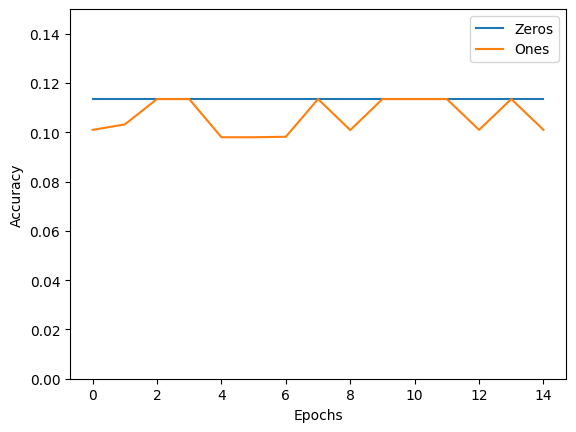
\includegraphics[scale=0.5]{img/01_MLP/first_initialize.png}
      \end{center}
      Clearly, this is not good, and theoretically this makes sense since it means all our activations are going to be the same, and thus all our gradients will be the same, meaning that are updates will be the same for every weight, which is not good mixing. We can see this below: 
    \end{example}

    \begin{example}[Random Initialization with High Variance]
      Okay, this didn't work, so perhaps you think it would be a good idea have more randomness to the initialization so that all the weights aren't exactly one number. You could think of initializing everything with three distinct schemes: 
      \begin{enumerate}[itemsep=0mm] 
        \item Randomly initialize everything to be $-1$ or $1$ with equal probability. 
        \item Randomly initialize everything to be a Gaussian random variable with standard deviation $1$. 
        \item Randomly initialize everything to be a uniform random variable between $-1$ and $1$. 
      \end{enumerate}
      Running the experiments give the following. 
      \begin{center} 
        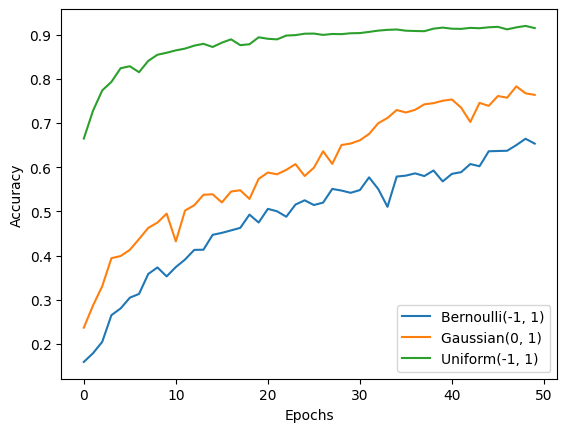
\includegraphics[scale=0.5]{img/01_MLP/second_initialization.png}
      \end{center}
      However, this is also not good since it means that the activations will be very large, and thus the gradients will be very large, and so the updates will be very large. This is not good since it means that the weights will be jumping around a lot, and we won't be able to converge. Furthermore, depending on what activations we choose, e.g. tanh or sigmoid, very large activations may saturate the gradients and kill the learning. 
    \end{example}

    \begin{example}[Random Initialization with Low Variance]
      This improves the next problem but now you want to fix the situation of the gradients being too big. Therefore, you should initialize the parameters to be smaller values, but not so small that they are zeros and we have the same problem as before. We use improved schemes: 
      \begin{enumerate}[itemsep=0mm] 
        \item Randomly initialize everything to be $-0.1$ or $0.1$ with equal probability. 
        \item Randomly initialize everything to be a Gaussian random variable with standard deviation $0.1$. 
        \item Randomly initialize everything to be a uniform random variable between $-0.1$ and $0.1$.
      \end{enumerate}
      \begin{center}
        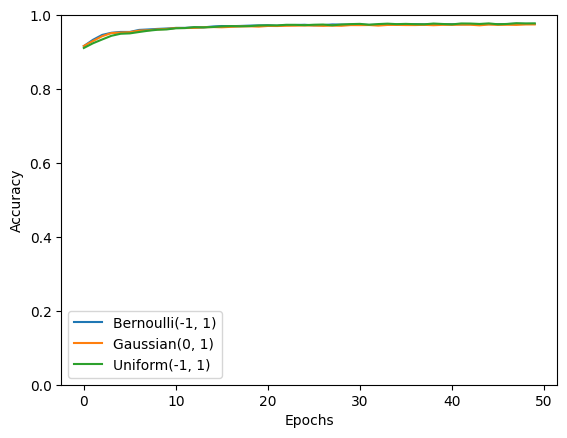
\includegraphics[scale=0.5]{img/01_MLP/third_initialize.png}
      \end{center}
    \end{example}

    Through out experiments, we have learned that a good rule of thumb for initializing weights is to make them small and uniformly random without being too small. While it is harder to get better than this for MNIST, a slightly better approach is Xavier initialization, which builds upon our same ideas. 

    \begin{definition}[Xavier Initialization]
      The \textbf{Xavier initialization} simply initializes each weight as a uniform distribution, with its range dependent on the size of the input. 
      \begin{equation}
        w_{ij}^{[l]} \sim U \bigg( -\frac{1}{\sqrt{N^{[l-1]}}}, \frac{1}{\sqrt{N^{[l-1]}}} \bigg)
      \end{equation}
      where $N^{[l-1]}$ is the number of neurons in the previous layer. This is a good rule of thumb for the weights, but the biases can be initialized to $0$ (though they are also initialized uniformly by default).
    \end{definition}

    \begin{code}[Experimenting with Weight Initializations] 
      The code used for generating the figures can be found \href{code/01_MLP/initialization.ipynb}{here}. 
    \end{code}
    
  \subsubsection{Activation Functions} 

    The choice of the activation function can have a significant impact on your training, and we will describe a few examples below. The first thing to note is that we must ensure that there is a nonzero gradient almost everywhere. If, for example, we had a piecewise constant activation function, the gradient is $0$ almost everywhere, and it would kill the gradient of the entire network. In the early days of deep learning, researchers used the probability-inspired sigmoid and tanh functions as the main source of nonlinearity. Let's go over them below. 

    \begin{definition}[Sigmoid]
      Sigmoid activations are historically popular since they have a nice interpretation as a saturating ``fire rate" of a neuron. However, there are 3 problems: 
      \begin{enumerate}
        \item The saturated neurons ``kill" the gradients, since if the input at any one point in the layers is too positive or negative, the gradient will vanish, making very small updates. This is known as the \textbf{vanishing gradient problem}. Therefore, the more layers a neural network has, the more likely we are to see this vanishing gradient problem. 
        \item Sigmoid functions are not zero centered (i.e. its graph doesn't cross the point $(0, 0)$ ). Consider what happens when the input $x$ to a neuron is always positive. Then, the sigmoid $f$ will have a gradient of 
        \begin{equation}
          f \bigg( \sum_i w_i x_i + b \bigg) \implies \frac{\partial f}{\partial w_i} = f^\prime \bigg( \sum_i w_i x_i + b \bigg)\, x_i
        \end{equation}
        which means that the gradients $\nabla_\mathbf{w} f$ will always have all positive elements or all negative elements, meaning that we will be restricted to moving in certain nonoptimal directions when updating our parameters. 
      \end{enumerate}
    \end{definition} 

    \begin{definition}[Hyperbolic Tangent]
      The hyperbolic tangent is zero centered, which is nice, but it still squashes numbers to range $[-1, 1]$ and therefore kills the gradients when saturated. 
    \end{definition}

    It turns out that these two activations were ineffective in deep learning due to saturation. A less probability inspired activation was the ReLU, which showed better generalization an speed of convergence. 

    \begin{definition}[Rectified Linear Unit]
      The ReLU function has the following properties: 
      \begin{enumerate}
          \item It does not saturate in the positive region. 
          \item It is very computationally efficient (and the fact that it is nondifferentiable at one point doesn't really affect computations). 
          \item It converges much faster than sigmoid/tanh in practice. 
          \item However, note that if the input is less than $0$, then the gradient of the ReLU is $0$. Therefore, if we input a vector that happens to have all negative values, then the gradient would vanish and we wouldn't make any updates. These ReLU ``dead zones" can be a problem since it will never activate and never update, which can happen if we have bad initialization. A more common case is when your learning rate is too high, and the weights will jump off the data manifold. 
      \end{enumerate}
    \end{definition}

    Unfortunately, the ReLU had some weaknesses, mainly being the \textit{dying ReLU}, which is when the ReLU is stuck in the negative region and never activates. This is a problem since the gradient is $0$ in the negative region, and so the weights will never update. Therefore, some researchers have proposed some modifications to the ReLU. 

    \begin{definition}[Leaky ReLU]
      The leaky ReLU 
      \begin{equation}
        \sigma(x) = \max\{0.01 x, x\}
      \end{equation}
      does not saturate (i.e. gradient will not die), is computationally efficient, and converges much faster than sigmoid/tanh in practice. We can also parameterize it with $\alpha$ and have the neural net optimize $\alpha$ along with the weights. 
      \begin{equation}
        \sigma(x) = \max\{\alpha x, x\}
      \end{equation}
    \end{definition}

    \begin{definition}[ELU]
      The exponential linear unit has all the benefits of ReLU, with closer to mean outputs. It has a negative saturation regime compared with leaky ReLU, but it adds some robustness to noise. 
      \begin{equation}
        \sigma(x) = \begin{cases} x & \text{ if } x > 0 \\ \alpha \big(\exp{x} - 1 \big) & \text{ if } x \leq 0 \end{cases}
      \end{equation}
    \end{definition}

    \begin{definition}[SELU]
      The scaled exponential linear unit is a self-normalizing activation function, which means that it preserves the mean and variance of the input. This is useful for deep networks, since the mean and variance of the input will be preserved through the layers. Its formula is 
      \begin{equation}
        \sigma(x) = \lambda \begin{cases} x & \text{ if } x > 0 \\ \alpha \big(\exp{x} - 1 \big) & \text{ if } x \leq 0 \end{cases}
      \end{equation}
      where $\lambda$ and $\alpha$ are constants.
    \end{definition}
    
    Later on, some further modifications were made, such as the \textbf{Swish} and the \textbf{Mish} \cite{misra2020mish} activation functions. These functions have a distinctive negative concavity, unlike ReLU, which accounts for preservation of small negative weights.  

    \begin{definition}[Swish]
      The Swish activation function is defined as 
      \begin{equation}
        \sigma(x) = x \cdot \sigma(\beta x) 
      \end{equation}
      where $\beta$ is a parameter that can be learned. 
    \end{definition}

    \begin{definition}[Mish]
      The Mish activation function is defined as 
      \begin{equation}
        \sigma(x) = x \cdot \tanh(\ln(1 + \exp(x))) 
      \end{equation}
    \end{definition}

    \begin{code}[Generating Graphs] 
      Code used to generate these graphs are \href{code/01_MLP/activation_functions.ipynb}{here}.
    \end{code} 

  \subsection{Datasets and Dataloaders} 

    For here, we will go over some of the main datasets that are used in deep learning. 

    \begin{definition}[MNIST and Fashion MNIST]
      The MNIST dataset consists of 60k training images and 10k test images of handwritten digits. The Fashion MNIST dataset consists of 60k training images and 10k test images of clothing items. These are considered quite easy with the basic benchmarks: 
      \begin{enumerate} 
        \item Linear classifiers can reach past 90\% accuracy. 
        \item A 2 layer MLP can reach up to 97\% accuracy. 
        \item A CNN can reach up to 99\% accuracy. 
      \end{enumerate}
    \end{definition}

    \begin{definition}[CIFAR10 and CIFAR 100]
      The CIFAR10 dataset consists of 60k 32x32 color images in 10 classes, with 6k images per class. The CIFAR100 dataset consists of 60k 32x32 color images in 100 classes, with 600 images per class. These are considered quite hard with the basic benchmarks: 
      \begin{enumerate} 
        \item Linear classifiers can reach past 40\% accuracy. 
        \item A 2 layer MLP can reach up to 60\% accuracy. 
        \item A CNN can reach up to 80\% accuracy. 
      \end{enumerate}
    \end{definition}

    \begin{definition}[ImageNet]
      The ImageNet dataset, created at Stanford by Fei-Fei Li \cite{ImageNet}, consists of 1.2 million training images and 50k validation images in 1000 classes. This is considered very hard with the basic benchmarks. 
    \end{definition}

    Creating your own custom dataset with spreadsheets or images is easy.\footnote{https://pytorch.org/tutorials/beginner/data\_loading\_tutorial.html} Loading it to a dataloader that shuffles and outputs minibatches of data is trivial. However, when doing so, you should pay attention to a couple things. 
    \begin{enumerate} 
      \item Batch size: The dataloader stores the dataset (which can be several hundred GBs) in the drive, and extracts batches into memory for processing. You should set your batch sizes so that they can fit into the GPU memory, which is often smaller than the CPU memory. 
    \end{enumerate}

\subsection{Exercises} 

  \begin{exercise}[Tarokh, ECE685 2021 Midterm 1.1]
    Let $x \in \mathbb{R}$ denote a random variable with the following \textit{cumulative distribution function} 
    \begin{equation}
      F(x) = \exp \bigg( - \exp \bigg( - \frac{x - \mu}{\beta} \bigg) \bigg)
    \end{equation}
    where $\mu$ and $\beta > 0$ denote the location and scale parameters, respectively. Let $\mathcal{D} = \{x_1, \ldots, x_n\}$ be a set of $n$ iid observations of $x$. 
    \begin{enumerate}
      \item Write an equation for a cost function $L(\mu, \beta \mid \mathcal{D})$ whose minimization gives the maximum likelihood estimates for $\mu$ and $\beta$. 
      \item Compute the derivatives of $L(\mu, \beta \mid \mathcal{D})$ with respect to $\mu$ and $\beta$ and write a system of equations whose solution gives the MLEs of $\mu$ and $\beta$. 
    \end{enumerate}
  \end{exercise}
  \begin{solution}
    We can derive the PDF of the observation as 
    \begin{equation}
      f(x; \mu, \beta) = \frac{d F(x)}{dx} = \frac{1}{\beta} \exp \bigg\{ - \bigg( \frac{x - \mu}{\beta} + \exp \Big( - \frac{x - \mu}{\beta}\Big) \bigg) \bigg\}
    \end{equation}
    and the likelihood is then 
    \begin{equation}
      L(\mu, \beta \mid \mathcal{D}) = \prod_{i=1}^N \frac{1}{\beta} \exp \bigg\{ - \bigg( \frac{x^{(i)} - \mu}{\beta} + \exp \Big( - \frac{x^{(i)} - \mu}{\beta}\Big) \bigg) \bigg\}
    \end{equation}
    Rather than maximizing this likelihood, we minimize the negative log of it, defined as 
    \begin{equation}
      \ell(\mu, \beta \mid \mathcal{D}) = - \ln L(\mu, \beta \mid \mathcal{D}) = N \ln{\beta} + \frac{\sum_{i} x^{(I)} - N \mu}{\beta} + \sum_{i=1}^N \exp \Big( - \frac{x^{(i)} - \mu}{\beta} \Big)
    \end{equation}
    The derivatives of $\ell$ can be computed simply by using the derivative rules.  
    \begin{align}
      \frac{\partial \ell}{\partial \mu} & = - \frac{N}{\beta} + \frac{1}{\beta} \sum_{i=1}^N \exp \Big( - \frac{x^{(i)} - \mu}{\beta} \Big) \\
      \frac{\partial \ell}{\partial \beta} & = \frac{N}{\beta} - \frac{\sum_{i} x^{(i)} - N \mu}{\beta^2} + \frac{1}{\beta^2} \sum_{i=1}^N (x^{(i)} - \mu) \exp \Big( - \frac{x^{(i)} - \mu}{\beta} \Big)
    \end{align}
    and so the MLE estimates that minimizes $\ell$ can be found by setting the equations above equal to $0$. 
  \end{solution}

  \begin{exercise}[ECE 685 Fall 2021 Midterm 1.2]
    The figure depicts a simple neural network with one hidden layer. The inputs to the network are denoted by $x_1, x_2, x_3$, and the output is denoted by $y$. The activation functions of the neurons in the hidden layer are given by $h_1 (z) = \sigma(z), h_2 (z) = \tanh(z)$, and the output unit activation function is $g(z) = z$, where $\sigma(z) = \frac{1}{1 + \exp(-z)}$ and $\tanh(z) = \frac{\exp(z) - \exp(-z)}{\exp(z) + \exp(-z)}$ are the logistic sigmoid and hyperbolic tangent, respectively. The biases $b_1, b_2$ are added to the inputs of the neurons int he hidden layer before passing them through the activation functions. let 
    \begin{equation}
      \mathbf{w} = (b_1, b_2, w_{11}^{(1)}, w_{12}^{(1)}, w_{21}^{(1)}, w_{31}^{(1)}, w_{32}^{(1)}, w_1^{(2)}, w_2^{(2)})
    \end{equation}
    denote the vector of network parameters. 
    \begin{enumerate}
      \item Write the input output relation $y = f(x_1, x_2, x_3 ; \mathbf{w})$ in explicit form. 

      \item Let $\mathcal{D} = \{(x_{1, n}, x_{2, n}, x_{3, n})\}$ denote a training dataset of $N$ points where $y_n \in \mathbb{R}$ are labels of the corresponding data points. We want to estimate the network parameters $\mathbf{w}$ using $\mathcal{D}$ by minimizing the mean squared error loss 
      \begin{equation}
        L(\mathbf{w}) = \frac{1}{2} \sum_{n=1}^N \big( f(x_{1, n}, x_{2, n}, x_{3, n}; \mathbf{w}) - y_n \big)^2
      \end{equation}
      Compute the gradient of $L(\mathbf{w})$ with respect to the network parameters $\mathbf{w}$. 

      \item Write pseudo code for one iteration for minimizing $L(\mathbf{w})$ with respect to the network parameters $\mathbf{w}$ using SGD with learning rate $\eta > 0$. 
    \end{enumerate}

    \begin{center}
      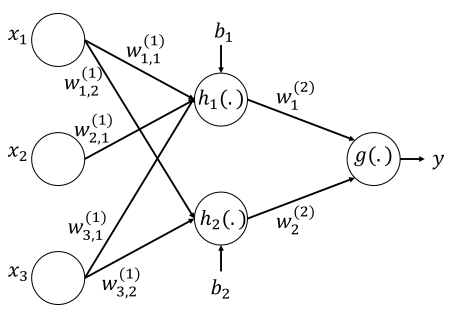
\includegraphics[scale=0.4]{img/01_MLP/tarokhfig1.png}
    \end{center}
  \end{exercise}
  \begin{solution}
    We can write the computation graph as 
    \begin{align} 
      z_1^{(1)} & = w_{11}^{(1)} x_1 + w_{21}^{(1)} x_2 + w_{31}^{(1)} x_3 + b_1 \\
      z_2^{(1)} & = w_{12}^{(1)} x_1 + w_{32}^{(1)} x_3 + b_2 \\
      a_1^{(1)} & = \sigma(z^{(1)})\\
      a_2^{(1)} & = \tanh(z_2^{(1)}) \\
      z^{(2)} & = w_{1}^{(2)} a_1^{(1)} + w_2^{(2)} a_2^{(1)} \\
      y = a^{(2)} & = g(z^{(2)})
    \end{align}
    and composing these gives 
    \begin{equation}
      y = w_1^{(2)} \sigma(w_{11}^{(1)} x_1  + w_{21}^{(1)} x_2 + w_{31}^{(1)} x_3 + b_1) + w_2^{(2)} \tanh(w_{12}^{(1)} x_1 + w_{32}^{(1)} x_3 + b_2)
    \end{equation}
    The gradient of the network can be written as 
    \begin{align}
      \nabla_\mathbf{w} L(\mathbf{w}) & = \frac{1}{2} \sum_{n=1}^N \nabla_\mathbf{w} \big( f(x_{1, n}, x_{2, n}, x_{3, n}; \mathbf{w}) - y_n \big)^2 \\
      & = \sum_{n=1}^N (f(x_{1, n}, x_{2, n}, x_{3, n}; \mathbf{w}) - y_n) \nabla_\mathbf{w} f(x_{1, n}, x_{2, n}, x_{3, n})
    \end{align}
    where 
    \begin{equation}
      \nabla_\mathbf{w} f(x_{1, n}, x_{2, n}, x_{3, n}) = \frac{\partial f}{\partial \mathbf{w}} \bigg|_{\mathbf{x} = \mathbf{x}^{(n)}}
    \end{equation}
    Now we can take derivatives using chain rule, working backwards, and using the derivative identities $\sigma^\prime (z)  = \sigma(z) (1 - \sigma(z))$ and $\tanh^\prime (z) = 1 - \tanh^2 (z)$. 
    \begin{align}
        \frac{\partial f}{\partial w_1^{(2)}} & = \frac{\partial f}{\partial z^{(2)}} \frac{\partial z^{(2)}}{\partial w_1^{(2)}} = a_1^{(1)} \\
        \frac{\partial f}{\partial w_2^{(2)}} & = \frac{\partial f}{\partial z^{(2)}} \frac{\partial z^{(2)}}{\partial w_2^{(2)}} = a_2^{(1)} \\ 
        \frac{\partial f}{\partial w_{11}^{(1)}} & = \frac{\partial f}{\partial z^{(2)}} \frac{\partial z^{(2)}}{\partial a^{(1)}_1} \frac{\partial a^{(1)}_1}{\partial z_1^{(1)}} \frac{\partial z_1^{(1)}}{\partial w_{11}^{(1)}} = w_1^{(2)} a_1^{(1)} (1 - a_1^{(1)}) x_1\\
        \frac{\partial f}{\partial w_{21}^{(1)}} & = \frac{\partial f}{\partial z^{(2)}} \frac{\partial z^{(2)}}{\partial a^{(1)}_1} \frac{\partial a^{(1)}_1}{\partial z_1^{(1)}} \frac{\partial z_1^{(1)}}{\partial w_{21}^{(1)}} = w_1^{(2)} a_1^{(1)} (1 - a_1^{(1)}) x_2\\
        \frac{\partial f}{\partial w_{31}^{(1)}} & = \frac{\partial f}{\partial z^{(2)}} \frac{\partial z^{(2)}}{\partial a^{(1)}_1} \frac{\partial a^{(1)}_1}{\partial z_1^{(1)}} \frac{\partial z_1^{(1)}}{\partial w_{31}^{(1)}} = w_1^{(2)} a_1^{(1)} (1 - a_1^{(1)}) x_3\\
        \frac{\partial f}{\partial b_{1}} & = \frac{\partial f}{\partial z^{(2)}} \frac{\partial z^{(2)}}{\partial a^{(1)}_1} \frac{\partial a^{(1)}_1}{\partial z_1^{(1)}} \frac{\partial z_1^{(1)}}{\partial b_{1}}  = w_1^{(2)} a_1^{(1)} (1 - a_1^{(1)}) \\
        \frac{\partial f}{\partial w_{12}^{(1)}} & = \frac{\partial f}{\partial z^{(2)}} \frac{\partial z^{(2)}}{\partial a^{(1)}_2} \frac{\partial a^{(1)}_2}{\partial z_2^{(1)}} \frac{\partial z_2^{(1)}}{\partial w_{12}^{(1)}} = w_2^{(2)} (1 - (a_2^{(1)})^2 ) x_1\\
        \frac{\partial f}{\partial w_{13}^{(1)}} & = \frac{\partial f}{\partial z^{(2)}} \frac{\partial z^{(2)}}{\partial a^{(1)}_2} \frac{\partial a^{(1)}_2}{\partial z_2^{(1)}} \frac{\partial z_2^{(1)}}{\partial w_{13}^{(1)}} = w_2^{(2)} (1 - (a_2^{(1)})^2 ) x_3 \\
        \frac{\partial f}{\partial b_{2}} & = \frac{\partial f}{\partial z^{(2)}} \frac{\partial z^{(2)}}{\partial a^{(1)}_2} \frac{\partial a^{(1)}_2}{\partial z_2^{(1)}} \frac{\partial z_2^{(1)}}{\partial b_{2}} = w_2^{(2)} (1 - (a_2^{(1)})^2 )
    \end{align}
    To compute one step of SGD, we must first choose a minibatch $\mathcal{M} \subset \mathcal{D}$ and then compute 
    \begin{equation}
      \nabla_{\mathbf{w}; \mathcal{M}} L(\mathbf{w}) = \sum_{(\mathbf{x}, y) \in \mathcal{M}} (f(\mathbf{x}; \mathbf{w}) - y) \nabla_{\mathbf{w}} f(\mathbf{x})
    \end{equation}
    where we compute the gradient simply over the minibatch. Then, we update the parameters according to 
    \begin{equation}
      \mathbf{w} = \mathbf{w} - \eta \nabla_{\mathbf{w}; \mathcal{M}} L(\mathbf{w})
    \end{equation}
  \end{solution}

  \begin{exercise}[ECE 685 Fall 2021 Midterm 1.3]
    Given the following neural network with 2 inputs $(x_1, x_2)$, fully-connected layers and ReLU activations. The weights and biases of hidden units are denoted $w$ and $b$, with $h$ as activation units. For example, 
    \begin{equation}
      h_1 = \mathrm{ReLU}(x_1 w_{11} + x_2 w_{21} + b_1)
    \end{equation}
    The outputs are denoted as $(y_1, y_2)$ and the ground truth targets are denoted as $(t_1, t_2)$. 
    \begin{equation}
      y_1  = \mathrm{ReLU} (h_1 w_{31} + h_2 w_{41} + b_3)
    \end{equation}
    \begin{center}
      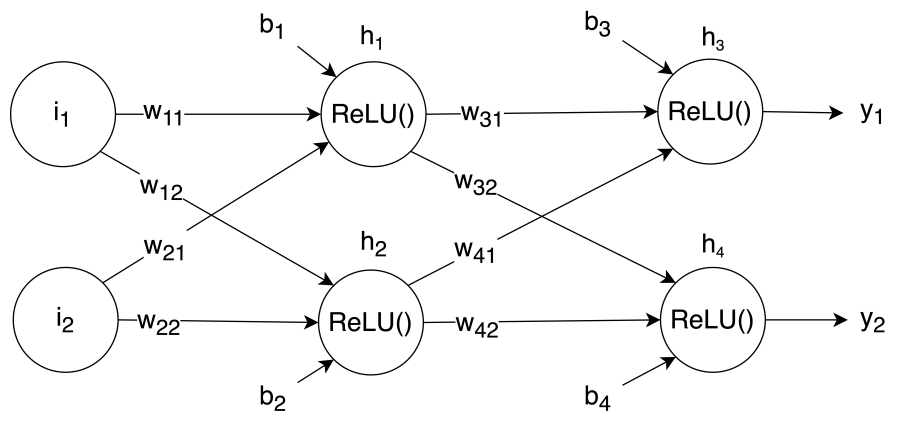
\includegraphics[scale=0.3]{img/01_MLP/nn_example.png} 
    \end{center}
    The values of the variables are given as follows: 
    \begin{table}[H]
      \centering
      \begin{tabular}{|c|c|c|c|c|c|c|c|c|c|c|c|c|c|c|c|}
        \hline
        $i_1$ & $i_2$ & $w_{11}$ & $w_{12}$ & $w_{21}$ & $w_{22}$ & $w_{31}$ & $w_{32}$ & $w_{41}$ & $w_{42}$ & $b_1$ & $b_2$ & $b_3$ & $b_4$ & $t_1$ & $t_2$ \\
        \hline
        1 & 2 & 1 & 0.5 & -0.5 & 1 & 0.5 & -2 & -1 & 0.5 & -0.5 & -0.5 & 1 & 1 & 2 & 4 \\
        \hline
      \end{tabular}
    \end{table}
    \begin{enumerate}
      \item Compute the output $(y_1, y_2)$ of the input $(x_1, x_2)$ using the network parameters as specified above. 
      \item Compute the mean squared error of the computed output and the target labels. 
      \item Using the calculated MSE, update the weight $w_{31}$ using GD with $\eta = 0.01$. 
      \item Do the same with weight $w_{42}$. 
      \item Do the same with weight $w_{22}$.  
    \end{enumerate}
  \end{exercise}

 
\section{Training and Control}

\subsection{Early Stopping}

  Since neural networks are overparameterized, it makes sense that given enough training time, they will overfit to the training set. Therefore, you must stop training when the validation loss starts to decrease. This simple method is known as \textbf{early stopping}. 

\subsection{L1 and L2 Regularization}

  Another way to regularize is by simply adding in a L1 or L2 regularization term. 

  Sometimes, it may not always be the best idea to regularize a neural net equally through all weights. For example, weights which may be deeper down the forward pass may focus on more high level features and therefore should be regularized differently than those that are close to the input. Other types of regularization, such as Fiedler regularization \cite{tam2020fiedler} focuses on preserving the graph structure of the weights. 

\subsection{Dropout}

  Overfitting is always a problem. With unlimited computation, the best way to regularize a fixed-sized mdoel is to average the predictions of all possible settings of the parameters, weighting each setting by its posterior probability given the training the data. However, this is computationally expensive and cannot be done for moderately complex models. 

  The dropout method introduced by \cite{srivastava14a}, addresses this issue. We literally drop out some features (not the weights!) before feeding them to the next layer by setting some activation functions to $0$. Given a neural net of $N$ total nodes, we can think of the set of its $2^N$ thinned subnetworks. For each training minibatch, a new thinned network is sampled and trained. 

  At each layer, recall that forward prop is basically 
  \begin{align*}
      \mathbf{z}^{[l+1]} & = \mathbf{W}^{[l+1]} \mathbf{a}^{[l]} + \mathbf{b}^{[l+1]} \\
      \mathbf{a}^{[l+1]} & = \boldsymbol{\sigma} (\mathbf{z}^{[l+1]}) 
  \end{align*}
  Now what we do with dropout is 
  \begin{align*}
      r_j^{[l]} & \sim \mathrm{Bernoulli}(p) \\
      \Tilde{\mathbf{a}}^{[l]} & = \mathbf{r}^{[l]} \odot \mathbf{a}^{[l]} \\
      \mathbf{z}^{[l+1]} & = \mathbf{W}^{[l+1]} \Tilde{\mathbf{a}}^{[l]} + \mathbf{b}^{[l+1]} \\
      \mathbf{a}^{[l+1]} & = \boldsymbol{\sigma} (\mathbf{z}^{[l+1]}) 
  \end{align*}
  Basically we a sample a vector of $0$s and $1$s from a multivariate Bernoulli distribtion. We element-wise multiply it with $\mathbf{a}^{[l]}$ to create the thinned output $\Tilde{\mathbf{a}}^{[l]}$. In test time, we do not want the stochasticity of having to set some activation functions to $0$. That is, consider the neuron $\mathbf{a}^{[l]}$ and the random variable $\Tilde{\mathbf{a}}^{[l]}$. The expected value of $\mathbf{z}^{[l+1]}$ is 
  \[\mathbb{E}[\mathbf{z}^{[l+1]}] = \mathbb{E}[ \mathbf{W}^{[l+1]} \Tilde{\mathbf{a}}^{[l]} + \mathbf{b}^{[l+1]}] = \mathbb{E}[ \mathbf{W}^{[l+1]} \Tilde{\mathbf{a}}^{[l]}] = p \mathbb{E}[\mathbf{W}^{[l+1]} \mathbf{a}^{[l]}] \]
  and to make sure that the output at test time is the same as the expected output at training time, we want to multiply the weights by $p$: $W^{[l]}_{\text{test}} = p \, W^{[l]}_{\text{train}}$. Another way is to use \textbf{inverted dropout}, where we can divide by $p$ in the training stage and keep the testing method the same. 

  \begin{code} 
    The code \href{code/02_Training/dropout.ipynb}{here} shows how to implement dropout in PyTorch, which uses dropout layers. 
  \end{code}

\subsection{Data Augmentation}

  It is well known that having more training data helps with overfitting, and so we may be able to perform basic transformations to our current data to artificially generate more training data. For example, if we have images, then we can flip, crop, translate, rotate, stretch, shear, and lens-distort these images with the same label. 

\subsection{Normalization Layers} 

  Just like how we have to normalize our data before we input into a linear model, it may help to normalize the outputs of one layer of a neural net before we input it into the next layer. This is an engineer's method to help with the training process. There are two ways that we can generally normalize data. First is to normalize each sample, known as \textbf{layer normalization}, and the other way is to normalize the samples over the batch. 

  \begin{definition}[Layer Norm]
    Given some batched output data $X \in \mathbb{R}^{b \times \mathbf{d}}$, where $b$ represents the batch size and $\mathbf{d} = d_1 \times \ldots \times d_k$ the dimension of each sample, we can normalize each $x_i = X_{i, :}$ in the batch with \textbf{layer normalization} by 
    \begin{equation}
      x_i \mapsto \frac{x_i - \mathbb{E}[x_i]}{\sqrt{\Var[x_i] + \varepsilon}} \odot \gamma + \beta
    \end{equation}
    where $\gamma, \beta$ are learnable parameters that are the same shape as $x_i$. If $X$ is of dimension $b \times \mathbf{d}$, we must use \texttt{nn.LayerNorm(d)} since these are the sizes of the learnable parameters. 
  \end{definition}

  \begin{example}[Layer Norm]
    The following example shows that each row (sample in batch) is normalized independently from one another. 
    \begin{lstlisting}
      ln = nn.LayerNorm(5)
      x = torch.Tensor(range(10)).reshape(2, 5)
      print(x)
      tensor([[0., 1., 2., 3., 4.],
              [5., 6., 7., 8., 9.]])

      print(ln(x))
      tensor([[-1.4142, -0.7071,  0.0000,  0.7071,  1.4142],
              [-1.4142, -0.7071,  0.0000,  0.7071,  1.4142]],
             grad_fn=<NativeLayerNormBackward0>)
    \end{lstlisting}
    This also works for higher dimensions. 
    \begin{lstlisting}
      ln = nn.LayerNorm((5, 2))
      x = torch.Tensor(range(20)).reshape(2, 5, 2)
      print(x)
      tensor([[[ 0.,  1.],
               [ 2.,  3.],
               [ 4.,  5.],
               [ 6.,  7.],
               [ 8.,  9.]],

              [[10., 11.],
               [12., 13.],
               [14., 15.],
               [16., 17.],
               [18., 19.]]])
      print(ln(x))
      tensor([[[-1.5667, -1.2185],
               [-0.8704, -0.5222],
               [-0.1741,  0.1741],
               [ 0.5222,  0.8704],
               [ 1.2185,  1.5667]],

              [[-1.5667, -1.2185],
               [-0.8704, -0.5222],
               [-0.1741,  0.1741],
               [ 0.5222,  0.8704],
               [ 1.2185,  1.5667]]], grad_fn=<NativeLayerNormBackward0>)
    \end{lstlisting}
    The tunable parameters $\gamma, \beta$ are indeed the same size. They are initialized to $1$s and $0$s. 
      \begin{lstlisting}
      >>> for k, v in ln.state_dict().items(): 
      ...     print(k, v)
      ... 
      weight tensor([[1., 1.],
              [1., 1.],
              [1., 1.],
              [1., 1.],
              [1., 1.]])
      bias tensor([[0., 0.],
              [0., 0.],
              [0., 0.],
              [0., 0.],
              [0., 0.]])
    \end{lstlisting}
  \end{example}

  \begin{definition}[Batch Norm]
    \textbf{Batch normalization} targets each feature over all batches rather than each sample (like columns vs rows). Therefore, given some batched output data $X \in \mathbb{R}^{b \times \mathbf{d}}$, where $b$ represents the batch size and $\mathbf{d} = d_1 \times \ldots \times d_k$ the dimension of each output, we can normalize each feature $x_i = X_{:,i \in \mathbf{d}}$ by 
    \begin{equation}
      x_i \mapsto \frac{x_i - \mathbb{E}[x_i]}{\sqrt{\Var[x_i] + \varepsilon}} \odot \gamma + \beta
    \end{equation}
    where $\gamma, \beta \in \mathbb{R}^b$ are learnable parameters that are the same size as the batch. There are two types of batch norms implemented in pytorch. 
    \begin{enumerate}
      \item If $X$ has hyperdimension $2$ with $b \times d$, we use \texttt{BatchNorm1d(d)} since we are normalizing over the batch for each feature and we have $d$ features to normalize. 
      \item If $X$ has hyperdimension $3$ with $b \times d_1 \times d_2$, we use \texttt{BatchNorm1d(d\_1)}. 
      \item If $X$ has hyperdimension $4$ with $b \times d_1 \times d_2 \times d_3$, we use \texttt{BatchNorm2d(d\_1)}. 
    \end{enumerate}
  \end{definition}

  \begin{example}[Batch Norm 1D]
    We can see that each feature is normalized independently from one another. For 2D, 
    \begin{lstlisting}
      >>> bn = nn.BatchNorm1d(5)
      >>> x = torch.Tensor(range(10)).reshape(2, 5)
      >>> print(x) 
      tensor([[0., 1., 2., 3., 4.],
              [5., 6., 7., 8., 9.]])
      >>> print(bn(x))
      tensor([[-1.0000, -1.0000, -1.0000, -1.0000, -1.0000],
              [ 1.0000,  1.0000,  1.0000,  1.0000,  1.0000]],
             grad_fn=<NativeBatchNormBackward0>)
    \end{lstlisting}
    For 3D inputs, 
    \begin{lstlisting}
      >>> bn = nn.BatchNorm1d(5)
      >>> x = torch.Tensor(range(30)).reshape(2, 5, 3)
      >>> print(x) 
      tensor([[[ 0.,  1.,  2.],
               [ 3.,  4.,  5.],
               [ 6.,  7.,  8.],
               [ 9., 10., 11.],
               [12., 13., 14.]],

              [[15., 16., 17.],
               [18., 19., 20.],
               [21., 22., 23.],
               [24., 25., 26.],
               [27., 28., 29.]]])
      >>> print(bn(x))
      tensor([[[-1.1267, -0.9941, -0.8616],
               [-1.1267, -0.9941, -0.8616],
               [-1.1267, -0.9941, -0.8616],
               [-1.1267, -0.9941, -0.8616],
               [-1.1267, -0.9941, -0.8616]],

              [[ 0.8616,  0.9941,  1.1267],
               [ 0.8616,  0.9941,  1.1267],
               [ 0.8616,  0.9941,  1.1267],
               [ 0.8616,  0.9941,  1.1267],
               [ 0.8616,  0.9941,  1.1267]]], grad_fn=<NativeBatchNo
      rmBackward0>)
    \end{lstlisting}
  \end{example}

  \begin{example}[Batch Norm 2D]
    Here is an example of batch norm 2d. There really isn't a difference between these two methods except the dimension that they take in. That is all. 
    \begin{lstlisting}
      >>> bn = nn.BatchNorm2d(5)
      >>> x = torch.Tensor(range(60)).reshape(2, 5, 3, 2)
      >>> print(x) 
      tensor([[[[ 0.,  1.],
                [ 2.,  3.],
                [ 4.,  5.]],
                ...
                [58., 59.]]]])
      >>> print(bn(x))
      tensor([[[[-1.1592, -1.0929],
                [-1.0267, -0.9605],
                ...
                [ 1.0929,  1.1592]]]], grad_fn=<NativeBatchNormBack
      ward0>)
    \end{lstlisting}
  \end{example}

\subsection{Residual Connections} 

  \begin{figure}[H]
    \centering 
    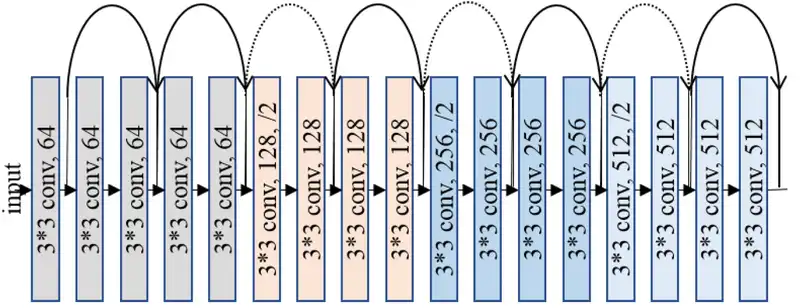
\includegraphics[scale=0.4]{img/02_Control/resnet_arch.png}
    \caption{Resnet architecture. } 
    \label{fig:resnet_arch}
  \end{figure}

  \begin{figure}[H]
    \centering 
    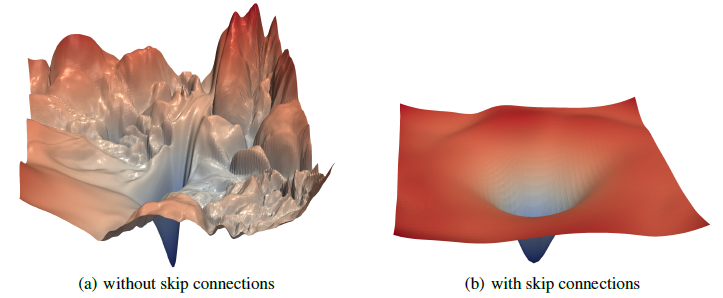
\includegraphics[scale=0.4]{img/02_Control/resnet_loss.png}
    \caption{Low-dimensional visual of loss with vs without residual connections. } 
    \label{fig:resnet_loss}
  \end{figure}

  \begin{figure}[H]
    \centering 
    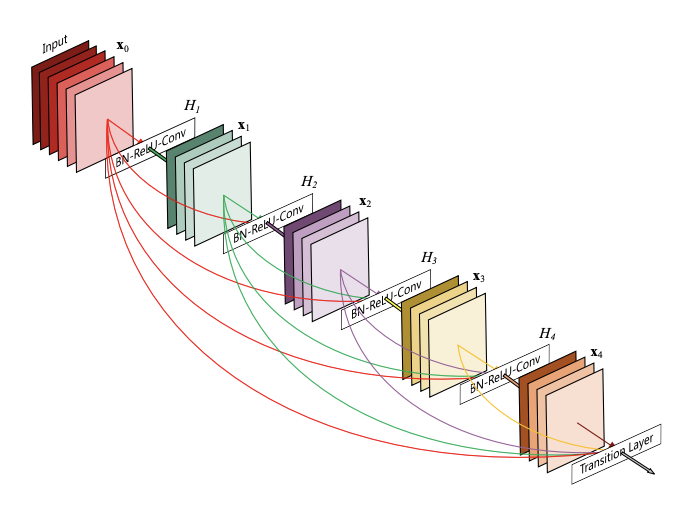
\includegraphics[scale=0.4]{img/02_Control/densenet.png}
    \caption{Densenet architecture. } 
    \label{fig:densenet_architecture}
  \end{figure}

\subsection{Network Pruning}

  It can be computationally and memory intensive to train and utilize neural networks. This is where network pruning comes in, which attempts to identify a subnetwork that performs as well as the original. Given a neural net $f(\mathbf{x}, \boldsymbol{\theta})$ where $\boldsymbol{\theta} \in \mathbb{R}^M$, a pruned neural network can be thought of as a subnetwork $f(\mathbf{x}, \mathbf{m} \odot \boldsymbol{\theta})$, where $\mathbf{m}$ is a \textbf{mask}, i.e. a vector in $\{0, 1\}^M$ that, when multiplied component-wise to $\boldsymbol{\theta}$, essentially ``deletes" a portion of the parameters. 
  \begin{center}
      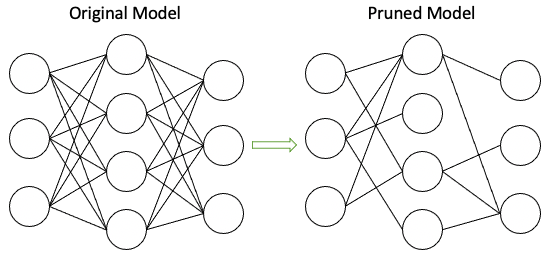
\includegraphics[scale=0.4]{img/02_Control/pruned_network.png}
  \end{center}
  This idea has been around for a long time, and the general method of pruning is as such: 
  \begin{enumerate}
      \item We initialize the neural network $f(\mathbf{x}, \boldsymbol{\theta}_0)$ and train it until we have $f(\mathbf{x}, \boldsymbol{\theta})$. 
      \item We now prune the network. The most basic pruning scheme is to keep the top $k\%$ largest weights, since smaller weights do not contribute much to the forward prop, and thus can be ignored. 
  \end{enumerate}
  These pruned networks have been shown to reach accuracies as high as the original network, with equal training progress. Now, if we were to take only this pruned network and train it from the beginning, it will perform as well as the original network, \textit{only under} the condition that we start from the same initialization $\mathbf{m} \odot \boldsymbol{\theta}$. If we take this subnetwork and initialize it differently at $\boldsymbol{\theta}_0^\prime$, then this subnetwork would not train well. Therefore, the performance of the pruned network is dependent on the initialization! 

  If we had initialized the full network differently, trained it, and then pruned again, we may have a different subnetwork that will only train well on its own given this new initialization. Therefore, a good initialization is extremely important for training subnetworks. This fact doesn't help much since we can't just take some arbitrary subnetwork and train it since we don't know the good initialization. We must always train the full network, then find the subnetwork, and then find its initialization. 

  This is essentially the \textbf{lottery ticket hypothesis} \cite{frankle2019lottery}, which states that a randomly-initialized, dense neural network contains a subnetwork that is initialized such that, when trained in isolation, it can match the test accuracy of the original network after training for at must the same number of iterations. 

  This paper hints at why neural networks work at all. It first states that only a very small subnetwork is responsible for the vast majority of its performance, but it must be initialized at the right position. But by overparameterizing these neural nets so much (by a certain margin), they have so many different combinations of subnetworks such that whatever initialization you throw at it, it is guaranteed that some subnetwork within it will train well with this initialization. This subnetwork is called the \textit{winning ticket}. 

\subsection{Curriculum Learning}

\subsection{Summary}

  Here is a few steps you can take as a guide to training a neural network.\footnote{From Stanford CS 229 NLP.}
  \begin{enumerate}
    \item Preprocess the data. 
    \item Choose your neural net architecture (number of layers/neurons, etc.) 
    \item Do a forward pass with the initial parameters, which should be small, and check that the loss is reasonable (e.g. $\log(1/10) \approx 2.3$ for softmax classification of 10 classes). 
    \item Now crank up the regularization term, and your loss should have gone up. 
    \item Now try to train on only a very small portion of your data without regularization using SGD, which you should be able to overfit and get the accuracy to 100\%. 
    \item Now you can train your whole dataset. Start off with a small regularization (e.g. 1e-6) and find a learning rate that makes the loss go down. 
    \begin{enumerate}
        \item Run for a few epochs to see if the cost goes down too slowly (step size is too small) or the cost explodes (step size too big). A general tip is that if the cost is ever bigger than $3$ times the original cost, then this is an indication that the cost has exploded. 
        \item We can run a grid search (in log space) over the learning rate and the regularization hyperparameters over say 10 epochs each, and compare which one makes the most progress. 
    \end{enumerate}
    \item Monitor and visualize the loss curve. 

    \begin{figure}[H]
      \centering 
      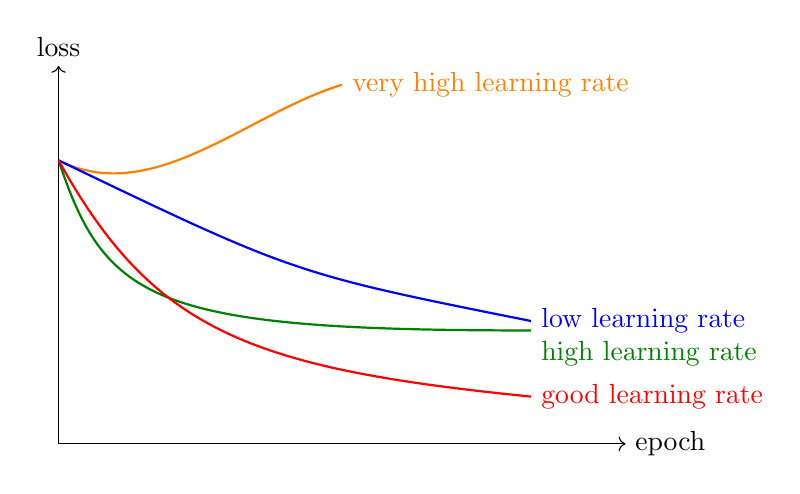
\begin{tikzpicture}[scale=1.2]
        % Set up the axes
        \draw[->] (0,0) -- (6,0) node[right] {epoch};
        \draw[->] (0,0) -- (0,4) node[above] {loss};
        
        % Plot the curves
        % Very high learning rate (yellow)
        \draw[orange, thick] (0,3) .. controls (1,2.5) and (2,3.5) .. (3,3.8) 
            node[right] {very high learning rate};
        
        % Low learning rate (blue)
        \draw[blue, thick] (0,3) .. controls (2.5, 1.8) .. (5,1.3) 
            node[right] {low learning rate};
        
        % High learning rate (green)
        \draw[green!50!black, thick] (0,3) .. controls (0.5,1.5) and (1,1.2) .. (5,1.2)
            node[below right] {high learning rate};
        
        % Good learning rate (red)
        \draw[red, thick] (0,3) .. controls (1,1.2) and (2,0.8) .. (5,0.5)
            node[right] {good learning rate};
      \end{tikzpicture}
      \caption{If you see loss curves that are flat for a while and then start decreasing, then bad initialization is a prime suspect. } 
      \label{fig:loss_curve_diagnostics}
    \end{figure}

    \item We also want to track the ratio of weight updates and weight magnitudes. That is, we can take the norm of the weights $\boldsymbol{\theta}$ and the gradient updates $\nabla \boldsymbol{\theta}$, and a rule of thumb is that the ratio should be about 
    \[\frac{||\nabla \boldsymbol{\theta}||}{||\boldsymbol{\theta}||} \approx 0.001 \text{ or } 0.01\]
  \end{enumerate}

 
\section{Convolutional Neural Networks}

  Convolutional networks work with images, so let's introduce a nice way to represent them as vectors. 

  \begin{definition}[Image]
    An image is a vector in some tensor product space. More specifically, avoiding the technicality that each pixel element is bounded and discrete, 

    \begin{enumerate}
      \item A \textbf{grayscale image} of resolution of $H \times W$ is a vector in $\mathbb{R}^{H} \otimes \mathbb{R}^{W}$. 
      \item An \textbf{image} with $C$ channels of the same resolution is an element of $\mathbb{R}^{C} \otimes \mathbb{R}^H \otimes \mathbb{R}^W$. 
      \item A \textbf{video} with $C$ channels and of the same resolution is an element of $\mathbb{R}^T \otimes \mathbb{R}^C \otimes \mathbb{R}^H \otimes \mathbb{R}^W$, where $T$ is the time dimension which is usually represented in some discrete frames.
    \end{enumerate} 
    Usually, we denote the height/width as the \textbf{spatial dimension}, the colors and the \textbf{channel dimension}, and time as the \textbf{temporal dimension}.\footnote{Everything we talked about so far applies to images when treated as vectors. In fact, so far we have been interpreting images of size $(C, H, W)$ through the isomorphism $\phi: \mathbb{R}^{C} \otimes \mathbb{R}^H \otimes \mathbb{R}^W \rightarrow \mathbb{R}^{C \times H \times W}$ that essentially ``unravels" the image. }
  \end{definition}

  Note that the terminology above is general convention, and tensors of arbitrary shape may exist that encode---say time over two dimensions. So far, we have seen the power of multilayer perceptrons and their predictive ability on moderately sized vectors. In fact, if we process the MNIST with a simple MLP of 2 layers and 512 nodes each, we can easily get $95\%$ accuracy within 10 epochs. However, these MNIST pictures are extremely low resolution, at $1 \times 28 \times 28$, and for even moderately sized images we can that there is a huge blowup of parameters needed. \footnote{For example, an RGB image that is $3 \times 1024 \times 1024$ would have ~3m parameters, and then defining a dense linear map to even 1000 dimensions would take 3 billion parameters. Given that 32-bit floating point is $4$ bytes, this already takes up 12GB of memory just to load the network.} Clearly, this is not efficient, and so the only way to move on is to create a sparser representation of the network. Therefore, can we create a sparser representation of a linear map that does sacrifice too much expressibility for memory? With convolutional kernels\footnote{Note that this is completely different than the kernels mentioned in supervised learning, with support vector machines and RKHS.}, the answer is yes. In 1994, Yann LeCunn and Yoshua Bengio in Bell Labs published \cite{cnn} which introduced the \textit{convolutional neural network}. 

\subsection{Convolutional and Pooling Layers} 

  The only layer know is a fully-connected layer. Now we will learn about our second type of layer. 

  \begin{definition}[1D Convolutional Layer]
    A \textbf{1D convolutional operator/layer} of 
    \begin{enumerate}
      \item input channels $C_{\mathrm{in}}$ 
      \item output channels $C_{\mathrm{out}}$ 
      \item kernel size $K$ 
      \item stride $S$
    \end{enumerate}
    is an operator $\phi: \mathbb{R}^{C_{\mathrm{in}}} \times \mathbb{R}^L \rightarrow \mathbb{R}^{C_{\mathrm{out}}} \times \mathbb{R}^{L_{\mathrm{out}}}$, where $C$ is the channel dimension and $L$ is the spatial dimension. We can view 
    \begin{equation}
      \phi(x)_{c, i} = \sum_{} 
    \end{equation}
  \end{definition}

  \begin{definition}[2D Convolutional Layer]
    A \textbf{convolutional operator/layer} of 
    \begin{enumerate}
      \item size 
    \end{enumerate}
  \end{definition}

  \begin{definition}[3D Convolutional Layer]
    A \textbf{convolutional operator/layer} of 
    \begin{enumerate}
      \item size 
    \end{enumerate}
  \end{definition}




  \begin{figure}[H]
    \centering 
    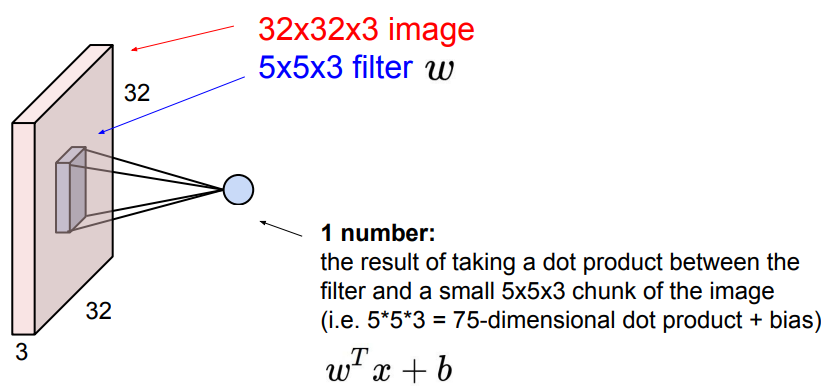
\includegraphics[scale=0.35]{img/kernel1.png}
    \caption{} 
    \label{fig:kernel1}
  \end{figure}

  \begin{figure}[H]
    \centering 
    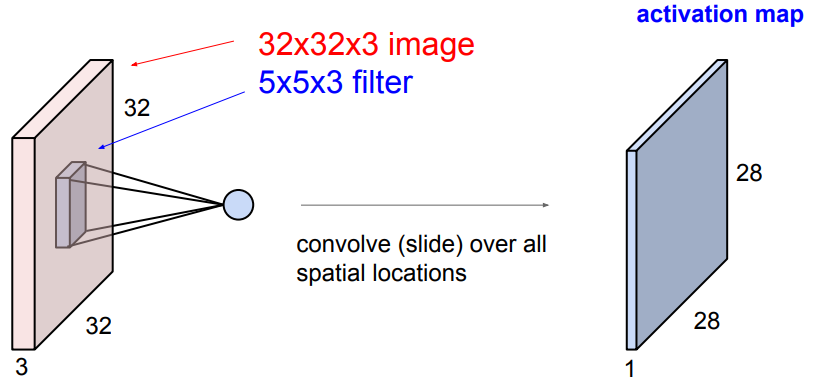
\includegraphics[scale=0.35]{img/kernel2.png}
    \caption{} 
    \label{fig:kernel2}
  \end{figure}

  \begin{figure}[H]
    \centering 
    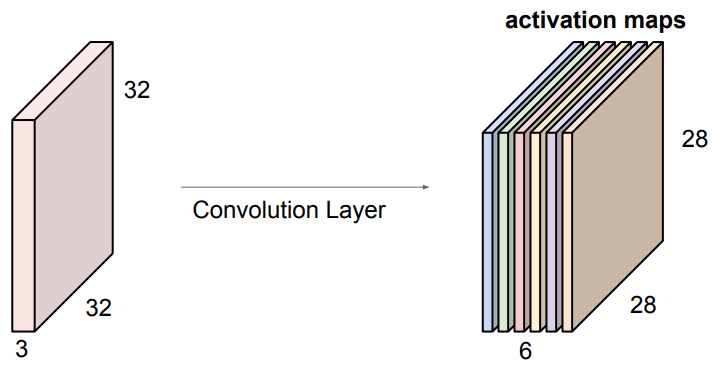
\includegraphics[scale=0.35]{img/kernel3.png}
    \caption{} 
    \label{fig:kernel3}
  \end{figure}

  \begin{definition}[Convolutional Kernel]
    A \textbf{convolution operator} on a vector space $V$ representing an image space is simply a special type of linear map that is parameterized by a much smaller set of numbers, stored within a \textbf{kernel} or \textbf{filter}. In all honesty, it is much easier to go through examples to see how they work, so in this definition I will focus more on describing the hyperparameters. Given an image of shape $(C, H, W)$, the convolution is essentially a sliding window that computes a dot product between the kernel and the window that the kernel covers over the image. 
    \begin{enumerate}
      \item The sliding window size is $(W_{ker}, H_{ker})$, which is conventionally square but does not need to be. 

      \item This sliding window must compute over all channels, so in fact it is of shape $(C_{in}, W_{ker}, H_{ker})$. This would generate one output channel image. 

      \item Multiple kernels can be used concurrently to generate different channel images. Therefore, if we want to have a collection of $C_{\text{out}}$ outputs that are extracted from each kernel, our total kernel would be a collection of $C_{out}$ kernels of shape $(C_{in}, W_{ker}, H_{ker}, C_{out})$. Therefore, the total equation is 
      \begin{equation}
        (X \ast K)_{f, i, j} \coloneqq \sum_c \sum_{p, q} X_{c, i + p, j + q} \cdot K_{c, p, q, f} + b_{f, i, j}
      \end{equation}

      where $c$ is the channel index, $p, q$ are the location indices, $f$ is the output channel index, and $b$ is some bias term. 

      \item The stride parameter $s$ can also be set to determine the stride of the kernel $\mathcal{K}$. 

      \item Another thing to note is that the output image of a kernel would be slightly smaller than the input image, since the kernel cannot go over the edge. However, there are padding schemes to preserve the original dimensions. 
    \end{enumerate}
    From the equation above, we can see that a convolutional layer, assuming that it has full padding, is a linear map  
    \begin{equation}
      \mathcal{K} : \mathbb{R}^{C_{in}} \otimes \mathbb{R}^H \otimes \mathbb{R}^W \rightarrow \mathbb{R}^{C_{out}} \otimes \mathbb{R}^H \otimes \mathbb{R}^W
      \label{eq:conv_mapping}
    \end{equation}
    The vector space of linear maps mapping between these two spaces has $C_{in} H^2 W^2 C_{out}$ dimensions, which is extremely large, but parameterizing $\mathcal{K}$ with this matrix reduces the set of relevant convolutional maps to a subspace that is $(1 + C_{in} H_{ker} W_{ker}) C_{out}$ dimensional (with the $+1$ due to a bias term, making this an affine map). This is essentially what a convolution is: sparse matrix multiplication, and there is nothing else that makes it different from a classical feedforward neural network. It's just computationally efficient matrix multiplication for high-dimensional vectors. 
  \end{definition}

  In addition to computational efficiency and weight sharing, convolutional operators capitalize on the principle of \textbf{locality}, i.e. that pixels are directly related to adjacent pixels. For example, a pixel representing a portion of a dog's ear would not be related to the background, but the color and positioning should be related to the dog's face, which may be within a certain neighborhood around. This has been shown to be similar to the human visual system and is thus well motivated. 

  Though this next topic has more to do with classical image processing than computer vision, there are a surprising number of features that these convolutional filters can extract from an image. By treating them as a discretized form of a partial derivative (as the vertical and horizontal edge detection) or as the Hessian operator (sharpening), we can extract many features from them.  

  \begin{example}[Blurs, Edge Detection]
    Given the original image below, we show various convolutional filters applied on the image. Note that the kernel matrix may have the property that all of its entries sum to $1$, meaning that on average, the expected value of the brightness of each pixel will be $0$, and the values will be left unchanged on average. However, this is not a requirement.  
    \begin{align*}
      \mathrm{Original} = \begin{bmatrix} 1 & 0 & 0 & 0 & 0 \\ 0 & 1 & 0 & 0 & 0 \\ 0 & 0 & 1 & 0 & 0 \\ 0 & 0 & 0 & 1 & 0 \\ 0 & 0 & 0 & 0 & 1 \end{bmatrix} & 
      \mathrm{Mean} = \frac{1}{25} \begin{bmatrix} 1 & 1 & 1 & 1 & 1 \\ 1 & 1 & 1 & 1 & 1 \\ 1 & 1 & 1 & 1 & 1 \\ 1 & 1 & 1 & 1 & 1 \\ 1 & 1 & 1 & 1 & 1 \end{bmatrix} & 
      \mathrm{Gaussian} = \frac{1}{273} \begin{bmatrix} 1 & 4 & 7 & 4 & 1 \\ 4 & 16 & 26 & 16 & 4 \\ 7 & 26 & 41 & 26 & 7 \\ 4 & 16 & 26 & 16 & 4 \\ 1 & 4 & 7 & 4 & 1 \end{bmatrix} \\   
      \mathrm{Sharpen} = \begin{bmatrix} 0 & -1 & 0 \\ -1 & 5 & -1 \\ 0 & -1 & 0 \end{bmatrix} & 
      \mathrm{Horizontal} = \begin{bmatrix} -1 & 0 & 1 \\ -2 & 0 & 2 \\ -1 & 0 & 1 \end{bmatrix} & 
      \mathrm{Vertical} = \begin{bmatrix} -1 & -2 & -1 \\ 0 & 0 & 0 \\ 1 & 2 & 1 \end{bmatrix} 
    \end{align*}

    These filters visually output the following images. Note that these filters are each acting on the image by acting individually on each channel and then combining the 3 outputs to create the new RGB image. 
    \begin{figure}[H]
      \centering
      \begin{subfigure}[b]{0.32\textwidth}
      \centering
          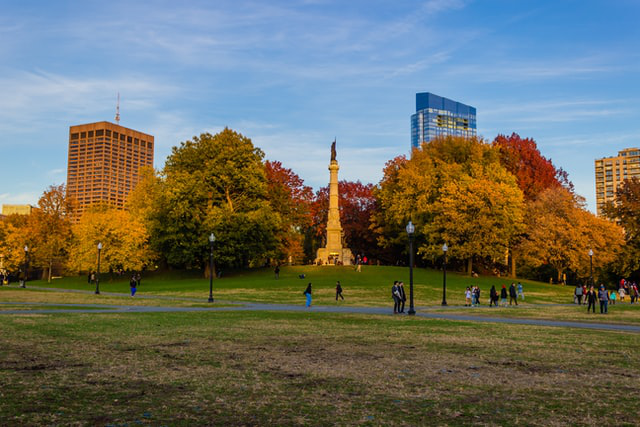
\includegraphics[width=\textwidth]{img/Park_Full.png}
          \caption{Original image. }
          \label{fig:original_image}
      \end{subfigure}
      \begin{subfigure}[b]{0.32\textwidth}
      \centering
          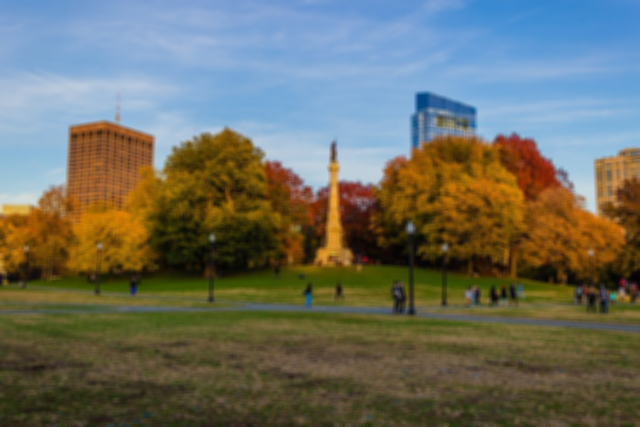
\includegraphics[width=\textwidth]{img/Mean_Blur.png}
          \caption{$5 \times 5$ mean blur applied. }
          \label{fig:mean_blur_image}
      \end{subfigure}
      \begin{subfigure}[b]{0.32\textwidth}
      \centering
          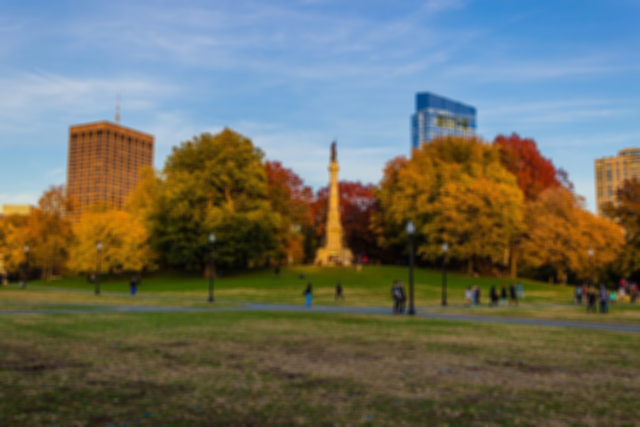
\includegraphics[width=\textwidth]{img/Gaussian_Blur.png}
          \caption{$5 \times 5$ Gaussian blur applied. }
          \label{fig:normal_blur_image}
      \end{subfigure}
      
      \begin{subfigure}[b]{0.32\textwidth}
      \centering
          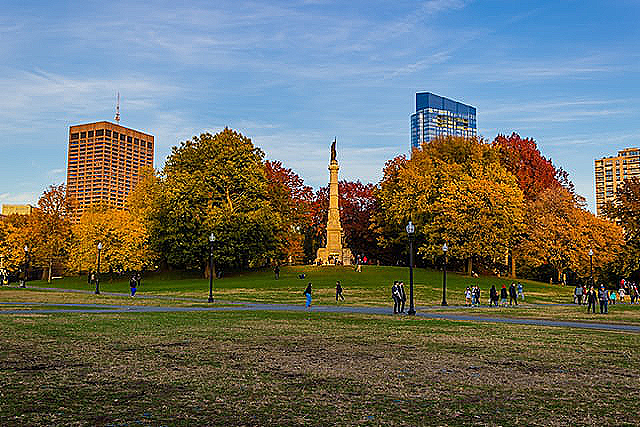
\includegraphics[width=\textwidth]{img/Sharpen.png}
          \caption{Sharpening kernel. } \label{fig:sharpened_image}
      \end{subfigure} 
      \begin{subfigure}[b]{0.32\textwidth}
      \centering
          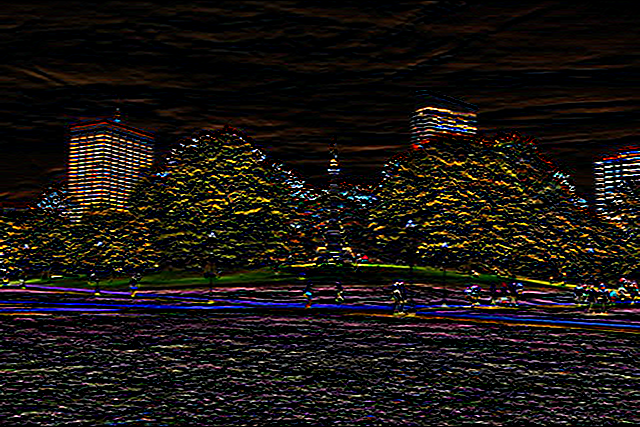
\includegraphics[width=\textwidth]{img/Horizontal.png}
          \caption{Horizontal edge detection. }
          \label{fig:horizontal_edge}
      \end{subfigure}
      \begin{subfigure}[b]{0.32\textwidth}
      \centering
          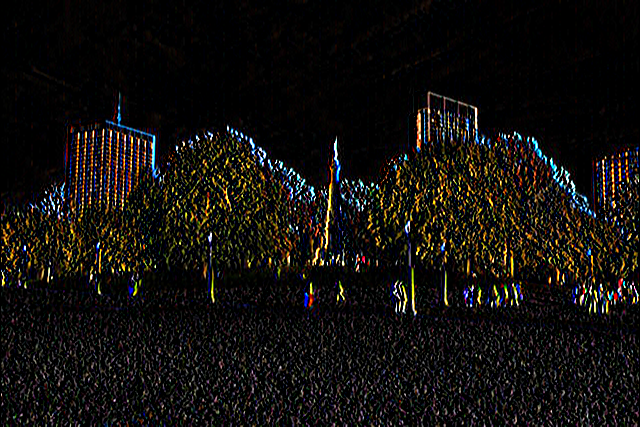
\includegraphics[width=\textwidth]{img/Vertical.png}
          \caption{Vertial edge detection. }
          \label{fig:vertical_edge}
      \end{subfigure} 

      \caption{Different convolutional kernels acting on the same image. Several useful features like edges can be detected with these simple linear maps. }
      \label{fig:feature_extraction}
    \end{figure}
  \end{example}

  We have seen in the example above that we can interpret each output channel of a convolution as a feature. That is, our original input image with $C_{in} = 3$ channels may go through a convolution that has $C_{out} = 10$ output channels, producing $10$ grayscale images. Each of these images may represent a feature that is extracted from the image through a custom kernel. When we stack convolutional layers together (with nonlinearities in between, of course), we can produce more complicated transformations that extract more abstract features. For example, while the first layer or two may extract certain edges within a dog, perhaps the fourth or fifth convolutional layer will be able to detect the presence of ears. This is a hand-wavy example, but if you actually visualize the outputs of these layers during forward prop, it is possible to see this in action.  

  What we eventually hope for is that we can extract higher level features that can be encoded in moderate-dimensional vectors. Unfortunately, the rate at which regular convolutional filters (especially when there is padding and a stride of $1$) does not shrink the resolution of the input images at a fast enough rate. For example, having a $3 \times 3 \times 3 \times 3$ kernel with no padding on a $(3, 100, 100)$ image will decrease the dimensions to only $(3, 98, 98)$ only. Therefore, we do some very simple operations to reduce the resolution faster. 

  \begin{figure}[H]
    \centering 
    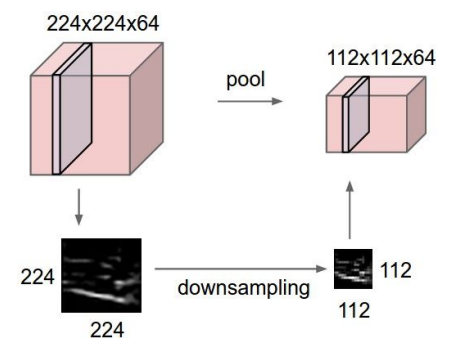
\includegraphics[scale=0.4]{img/max_pool1.png}
    \caption{} 
    \label{fig:max_pool1}
  \end{figure}

  \begin{figure}[H]
    \centering 
    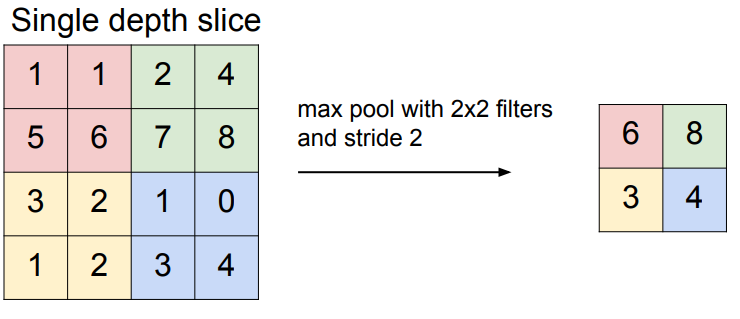
\includegraphics[scale=0.4]{img/max_pool2.png}
    \caption{} 
    \label{fig:max_pool2}
  \end{figure}

  \begin{definition}[Pooling Layers]
    A pooling layer takes in an input image of dimension $(C, H, W)$ and essentially does \textbf{downsampling} on it, involving some method of pooling local groups of pixels together into one value. There are several ways to do this: 
    \begin{enumerate}
      \item \textbf{Max Pooling} refers to dividing each channel of the image into a ``checkerboard" of $P \times P$ (where $P$ is a hyperparameter and does not necessarily have to be a square) matrices and simply choosing the maximum pixel value from it. 
      \item \textbf{Average Pooling} is the same as max pooling but we just take the average. 
    \end{enumerate}
    Clearly, these are not expensive operations and are an effective way to downsample. Therefore, the same $(3, 100, 100)$ image, after one convolutional layer followed by a pooling layer, will result in a $(3, 49, 49)$ image.  
  \end{definition}

  Ultimately, after a series of convolutions and pooling, we would want to reduce this image to a form of $(C, H, W)$, where both $H$ and $W$ are small and $C$ is large. This is because for each value of $C$, say $C = 1$, the cross section $\{(1, W, H)\}$ would encode the value of the feature identified by $C$. In fact, it could be the fact that both $H$ and $W$ are $1$, and $C = 10$. Then, we would essentially be looking at an array of $10$ numbers, which could encode the presence of some abstract features. For example, the first value $C = 1$ would encode the presence of an eye, which in the end has a value of $0.9$ (high probability), the second $C = 2$ could encode the presence of an ear, and so on. 

  Perhaps the sparsity of these maps may not allow the convolutional layers alone to extract all the features we need, so it is common to unwrap the features and then add a few fully connected layers at the end, which is much more computationally feasible now that the convolutions and pooling layers have reduced the dimensionality whilst extracting useful features with the concept of locality. This turns out to have comparable performance to regular MLPs with a fraction of the computational cost, and can easily reach $98\%$ validation accuracy on the MNIST dataset. 

  \begin{center}
    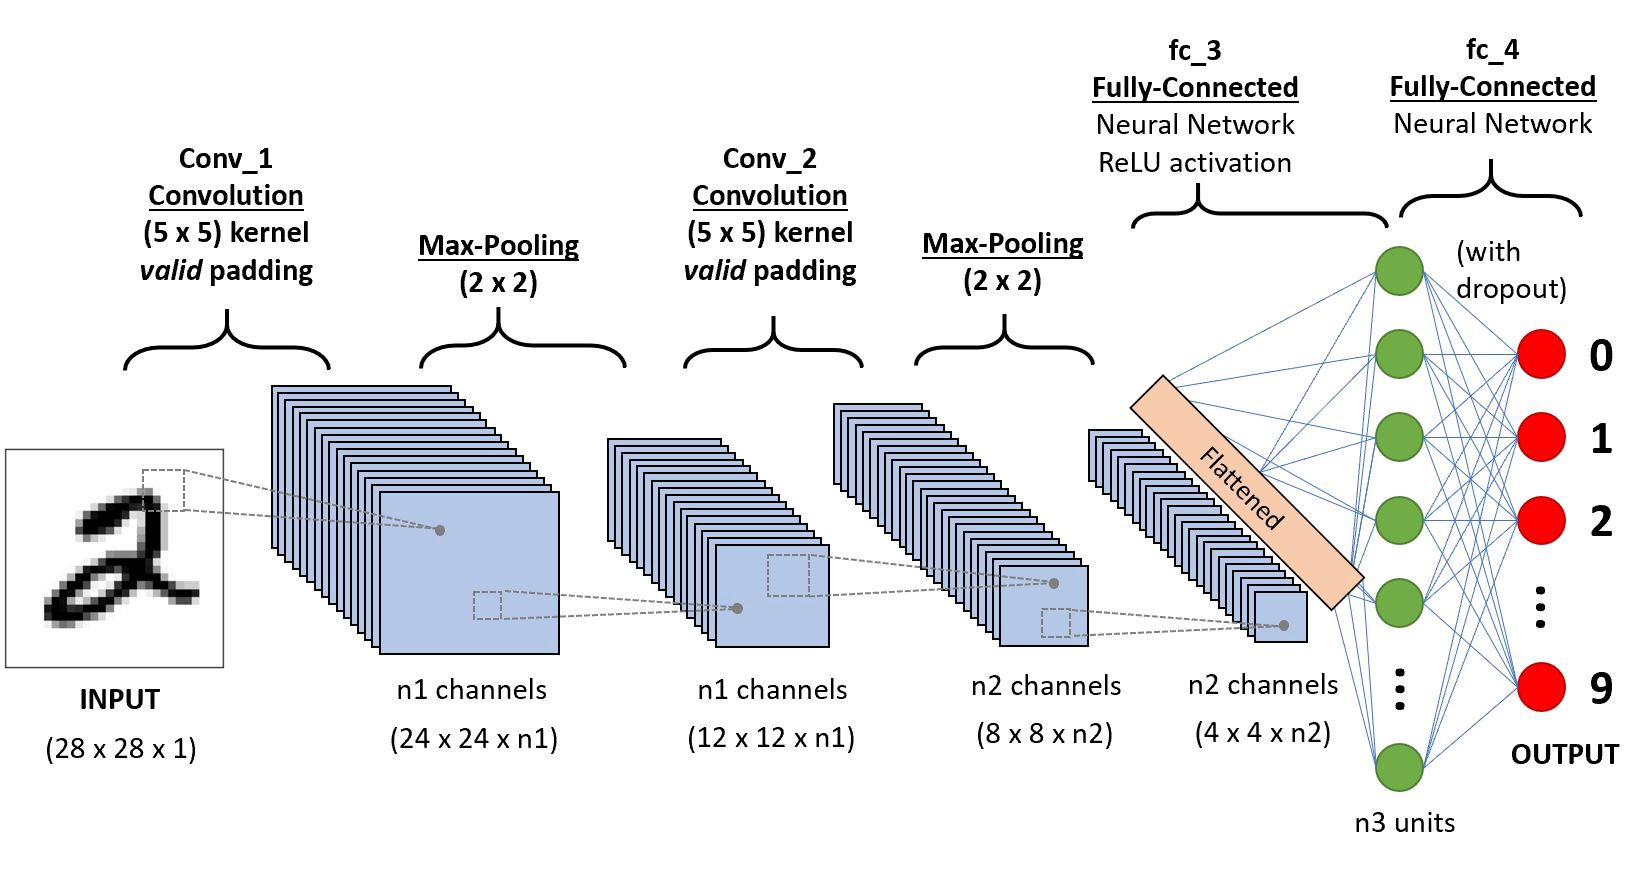
\includegraphics[scale=0.25]{img/CNN_architecture.jpeg}
  \end{center}

\subsection{Backpropagation}

  The fully connected layers are all taken care of, but now it's the convolutional layers and the pooling layers. The convolutional layers are also linear maps, so they can be treated the same way. However, the pooling layers may be nonlinear. 
  \begin{enumerate}
    \item Average pooling is linear, so no worries here. 
    \item Max pooling is not linear, but it is the next best thing: piecewise linear. 
  \end{enumerate}

\subsection{Visualizing Activation Maps}

  \subsection{CAM and Grad-CAM}


\subsection{Exercises}

  \begin{example}[Tarokh, Duke ECE685]
    Consider an RGB image $X = [X_0, X_1, X_2]$ with three channels, and given as follows 

    \begin{equation}
      X_0 = \begin{bmatrix} 2 & 1 & 0 & 0 \\ 0 & 0 & 2 & 1 \\ 0 & 2 & 0 & 1 \\ 2 & 1 & 0 & 1 \end{bmatrix}, \;\; 
      X_1 = \begin{bmatrix} 2 & 2 & 0 & 0 \\ 0 & 0 & 2 & 1 \\ 0 & 0 & 2 & 0 \\ 0 & 1 & 0 & 1 \end{bmatrix}, \;\; 
      X_2 = \begin{bmatrix} 2 & 1 & 0 & 0 \\ 0 & 0 & 2 & 1 \\ 2 & 0 & 0 & 0 \\ 0 & 1 & 0 & 1 \end{bmatrix}
      \label{eq:tarokh_conv_exercise}
    \end{equation}
    
    The image is passed through the convolutional filter with the weights $W = [W_0, W_1, W_2] \in \mathbb{R}^{3 \times 3 \times 3}$ and step size $1$, and given as follows 

    \begin{equation}
      W_0 = \begin{bmatrix} 1 & 0 & 0 \\ 0 & -2 & 0 \\ 0 & 0 & -1 \end{bmatrix}, \;\; 
      W_1 = \begin{bmatrix} 1 & 2 & 0 \\ 2 & 0 & - 1 \\ 0 & -1 & 1 \end{bmatrix}, \;\; 
      W_2 = \begin{bmatrix} 0 & 0 & -2 \\ 0 & 1 & 2 \\ -2 & 2 & 0 \end{bmatrix} 
      \label{eq:tarokh_conv_exercise2}
    \end{equation}   

    The output of the convolutional filter is given as 
    \begin{equation}
      Y = \mathrm{ReLU} \bigg( \sum_{i=0}^2 (X_i^\prime \ast W_i) + 2 \cdot 1_{4 \times 4}\bigg)
    \end{equation}
    where $Y$ is the output image, $X^\prime$ is the input image after applying $0$ padding around the edges, and $\ast$ is the discrete convolution operator. Compute the output $Y$, and then apply max pooling on nonoverlapping $2 \times 2$ submatrices, and then apply average pooling on non-overlapping $2 \times 2$ submatrices. 
  \end{example}
  \begin{solution}
    We can compute 
    \begin{align*} 
      X_0 \ast  W_0 & = \begin{bmatrix} -4 & -4 & -1 & 0 \\ -2 & 2 & -4 & -2 \\ -1 & -4 & -1 & 0 \\ -4 & -2 & 2 & -2 \end{bmatrix} \\
      X_1 \ast W_1 & = \begin{bmatrix} -2 & 6 & 3 & -1 \\ 4 & 6 & -1 & 4 \\ 1 & -3 & 5 & 7 \\ -1 & 0 & 5 & 2 \end{bmatrix} \\
      X_2 \ast W_2 & = \begin{bmatrix} 4 & 1 & 4 & -2 \\ 2 & 0 & 4 & 11 \\ 2 & -2 & -4 & 2 \\ 2 & 1 & 2 & 1 \end{bmatrix}
    \end{align*}
    and so we get 
    \begin{equation}
      Y = \begin{bmatrix} 0 & 5 & 8 & 0 \\ 6 & 10 & 1 & 5 \\ 4 &  0 & 2 & 11 \\ 0 & 1 & 11 & 3 \end{bmatrix}
    \end{equation}
    Maxpooling and average pooling gives us 
    \begin{equation}
      \mathrm{max}(Y) = \begin{bmatrix} 10 & 8 \\ 4 & 11 \end{bmatrix} \text{ and } \mathrm{avg}(Y) = \begin{bmatrix} 21/4 & 7/2 \\ 5/4 & 27/4 \end{bmatrix}
    \end{equation}
  \end{solution}


\section{Recurrent Neural Networks}

  Let's focus on what is lacking in the vanilla feedforward neural net architecture. In a vanilla feedforward neural net architecture, we had a one to one map, where we take an input of fixed size and we map it to an output of fixed size. Perhaps we would want a one-to-many model, which takes in an image for example and outputs a variable-length description of the image. Or a many-to-many (e.g. machine translation from a sequence of words to a sequence of words) or many-to-one. Just as a convolutional neural network is specialized for processing a grid a values such as an image, a recurrent neural network is specialized for processing a sequence of values (e.g. audio, video, text, speech, time series). 

  \begin{figure}[H]
    \centering 
    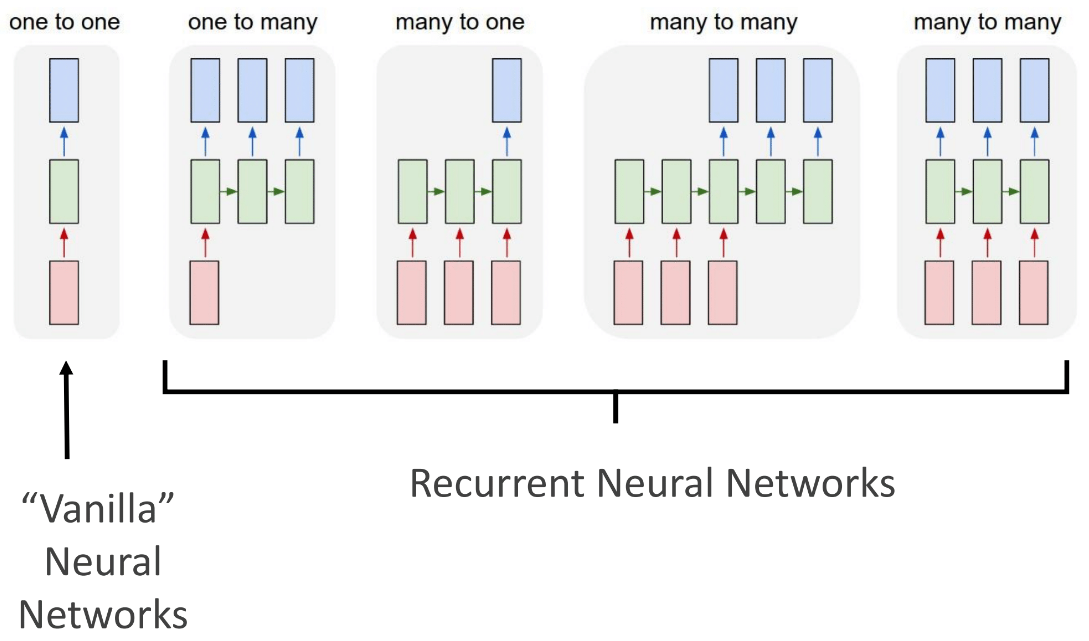
\includegraphics[scale=0.25]{img/NNs_vs_RNN.png}
    \caption{It is not limited to a fixed size of inputs and outputs.} 
    \label{fig:rnns}
  \end{figure}

  Now to build such a model where the input or output elements are unbounded, we must take advantage of \textit{weight sharing} (as seen in the CNN architecture) to control the size of our neural net. Furthermore, the fact that we should take in a sequence of inputs means that we may want to introduce some recursive structure in our neural net. Consider the classical form of a dynamical system driven by an external signal $\mathbf{x}$ as 
  \begin{equation}
    \mathbf{s}_t = f(\mathbf{s}_{t-1}, \mathbf{x}_t; \, \boldsymbol{\theta} )
  \end{equation}
  which defines a recurrent relationship. Similarly, we can write $\mathbf{h}$ to represent hidden neurons and write 
  \begin{equation}
    \mathbf{h}_t = f(\mathbf{h}_{t-1}, \mathbf{x}_t; \, \boldsymbol{\theta} )
  \end{equation}
  which indicates that the state of a hidden neuron is dependent on both the previous neuron and an input at time $t$. Through recursion, the hidden state $\mathbf{h}_t$ contains all information about the inputs $\mathbf{x}_1, \ldots, \mathbf{x}_t$ in the form of a complex function $\mathbf{g}$. 
  \begin{align}
      \mathbf{h}_t & = \mathbf{g}_t \big( \mathbf{x}_t, \mathbf{x}_{t - 1}, \ldots, \mathbf{x}_1 \big) \\
      & = f(\mathbf{h}_{t - 1}, \mathbf{x}_t; \, \boldsymbol{\theta}) 
  \end{align}
  The fact that we can factorize $\mathbf{g}_t$ into a repeated application of function $\mathbf{f}$ gives us two advantages: 
  \begin{enumerate}
      \item Regardless of the sequence length, the learned model always has the same input size because it is specified in terms of transition from one state to another state, rather than specified in terms of a variable-length history of states. 

      \item It is possible to use the same transition function $f$ with the same parameters at every time step. Since we do not have a growing number of parameters to optimize as our sequential data grows, training an RNN is still computationally feasible. 
  \end{enumerate}
  These two factors make it possible to learn a single model $f$ that operates on all time steps and all sequence lengths, rather than needing to learn a separate model $\mathbf{g}_t$ for all possible time steps. 

\subsection{Unidirectional RNNs}

  A single layer unidirectional RNN is a direct application of the idea mentioned in the previous section. We can first look at its computational graph 

  \begin{figure}[H]
    \centering 
    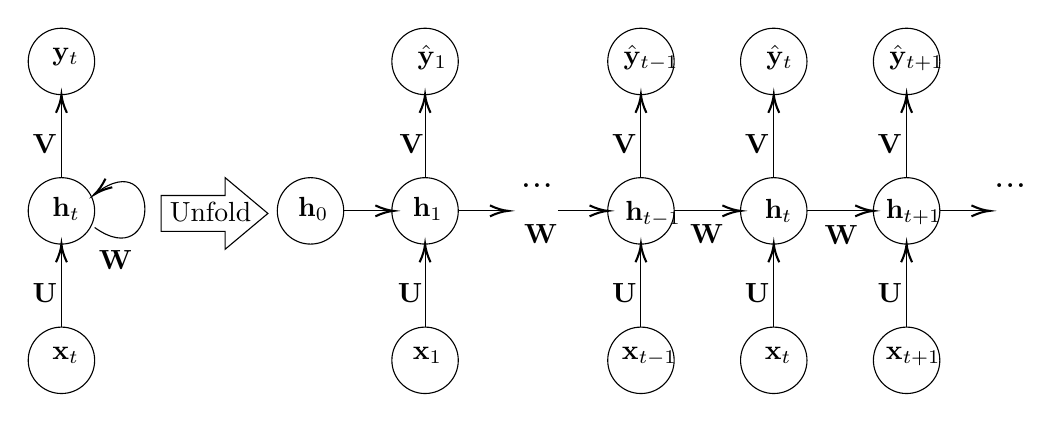
\begin{tikzpicture}[x=0.75pt,y=0.75pt,yscale=-0.8,xscale=0.8]
      %Shape: Ellipse [id:dp5130048407384993] 
      \draw   (40,30) .. controls (40,18.95) and (48.95,10) .. (60,10) .. controls (71.05,10) and (80,18.95) .. (80,30) .. controls (80,41.05) and (71.05,50) .. (60,50) .. controls (48.95,50) and (40,41.05) .. (40,30) -- cycle ;
      %Shape: Ellipse [id:dp17480372599276373] 
      \draw   (389,30) .. controls (389,18.95) and (397.95,10) .. (409,10) .. controls (420.05,10) and (429,18.95) .. (429,30) .. controls (429,41.05) and (420.05,50) .. (409,50) .. controls (397.95,50) and (389,41.05) .. (389,30) -- cycle ;
      %Shape: Ellipse [id:dp5960411091761506] 
      \draw   (549,30) .. controls (549,18.95) and (557.95,10) .. (569,10) .. controls (580.05,10) and (589,18.95) .. (589,30) .. controls (589,41.05) and (580.05,50) .. (569,50) .. controls (557.95,50) and (549,41.05) .. (549,30) -- cycle ;
      %Shape: Ellipse [id:dp7206562814926485] 
      \draw   (469,30) .. controls (469,18.95) and (477.95,10) .. (489,10) .. controls (500.05,10) and (509,18.95) .. (509,30) .. controls (509,41.05) and (500.05,50) .. (489,50) .. controls (477.95,50) and (469,41.05) .. (469,30) -- cycle ;
      %Curve Lines [id:da10598972243494376] 
      \draw [color={rgb, 255:red, 0; green, 0; blue, 0 }  ,draw opacity=1 ]   (80,130) .. controls (119.93,158.71) and (120.33,79.61) .. (81.2,109.07) ;
      \draw [shift={(80,110)}, rotate = 321.57] [color={rgb, 255:red, 0; green, 0; blue, 0 }  ,draw opacity=1 ][line width=0.75]    (10.93,-3.29) .. controls (6.95,-1.4) and (3.31,-0.3) .. (0,0) .. controls (3.31,0.3) and (6.95,1.4) .. (10.93,3.29)   ;
      %Right Arrow [id:dp18992895807915655] 
      \draw   (120,110.77) -- (158.6,110.77) -- (158.6,100) -- (184.34,121.55) -- (158.6,143.1) -- (158.6,132.32) -- (120,132.32) -- cycle ;
      %Shape: Ellipse [id:dp5707409054176504] 
      \draw   (40,120) .. controls (40,108.95) and (48.95,100) .. (60,100) .. controls (71.05,100) and (80,108.95) .. (80,120) .. controls (80,131.05) and (71.05,140) .. (60,140) .. controls (48.95,140) and (40,131.05) .. (40,120) -- cycle ;
      %Shape: Ellipse [id:dp7312065482605519] 
      \draw   (389,120) .. controls (389,108.95) and (397.95,100) .. (409,100) .. controls (420.05,100) and (429,108.95) .. (429,120) .. controls (429,131.05) and (420.05,140) .. (409,140) .. controls (397.95,140) and (389,131.05) .. (389,120) -- cycle ;
      %Shape: Ellipse [id:dp09029880081936525] 
      \draw   (549,120) .. controls (549,108.95) and (557.95,100) .. (569,100) .. controls (580.05,100) and (589,108.95) .. (589,120) .. controls (589,131.05) and (580.05,140) .. (569,140) .. controls (557.95,140) and (549,131.05) .. (549,120) -- cycle ;
      %Shape: Ellipse [id:dp3877188933189881] 
      \draw   (469,120) .. controls (469,108.95) and (477.95,100) .. (489,100) .. controls (500.05,100) and (509,108.95) .. (509,120) .. controls (509,131.05) and (500.05,140) .. (489,140) .. controls (477.95,140) and (469,131.05) .. (469,120) -- cycle ;
      %Shape: Ellipse [id:dp56230914391766] 
      \draw   (259,120) .. controls (259,108.95) and (267.95,100) .. (279,100) .. controls (290.05,100) and (299,108.95) .. (299,120) .. controls (299,131.05) and (290.05,140) .. (279,140) .. controls (267.95,140) and (259,131.05) .. (259,120) -- cycle ;
      %Straight Lines [id:da6793613738120752] 
      \draw [color={rgb, 255:red, 0; green, 0; blue, 0 }  ,draw opacity=1 ]   (299,120) -- (327,120) ;
      \draw [shift={(329,120)}, rotate = 180] [color={rgb, 255:red, 0; green, 0; blue, 0 }  ,draw opacity=1 ][line width=0.75]    (10.93,-3.29) .. controls (6.95,-1.4) and (3.31,-0.3) .. (0,0) .. controls (3.31,0.3) and (6.95,1.4) .. (10.93,3.29)   ;
      %Straight Lines [id:da07841792239013201] 
      \draw [color={rgb, 255:red, 0; green, 0; blue, 0 }  ,draw opacity=1 ]   (359,120) -- (387,120) ;
      \draw [shift={(389,120)}, rotate = 180] [color={rgb, 255:red, 0; green, 0; blue, 0 }  ,draw opacity=1 ][line width=0.75]    (10.93,-3.29) .. controls (6.95,-1.4) and (3.31,-0.3) .. (0,0) .. controls (3.31,0.3) and (6.95,1.4) .. (10.93,3.29)   ;
      %Straight Lines [id:da17044753691104964] 
      \draw [color={rgb, 255:red, 0; green, 0; blue, 0 }  ,draw opacity=1 ]   (429,120) -- (467,120) ;
      \draw [shift={(469,120)}, rotate = 180] [color={rgb, 255:red, 0; green, 0; blue, 0 }  ,draw opacity=1 ][line width=0.75]    (10.93,-3.29) .. controls (6.95,-1.4) and (3.31,-0.3) .. (0,0) .. controls (3.31,0.3) and (6.95,1.4) .. (10.93,3.29)   ;
      %Straight Lines [id:da6051247889848512] 
      \draw [color={rgb, 255:red, 0; green, 0; blue, 0 }  ,draw opacity=1 ]   (509,120) -- (547,120) ;
      \draw [shift={(549,120)}, rotate = 180] [color={rgb, 255:red, 0; green, 0; blue, 0 }  ,draw opacity=1 ][line width=0.75]    (10.93,-3.29) .. controls (6.95,-1.4) and (3.31,-0.3) .. (0,0) .. controls (3.31,0.3) and (6.95,1.4) .. (10.93,3.29)   ;
      %Straight Lines [id:da2538393669251706] 
      \draw [color={rgb, 255:red, 0; green, 0; blue, 0 }  ,draw opacity=1 ]   (589,120) -- (617,120) ;
      \draw [shift={(619,120)}, rotate = 180] [color={rgb, 255:red, 0; green, 0; blue, 0 }  ,draw opacity=1 ][line width=0.75]    (10.93,-3.29) .. controls (6.95,-1.4) and (3.31,-0.3) .. (0,0) .. controls (3.31,0.3) and (6.95,1.4) .. (10.93,3.29)   ;
      %Shape: Ellipse [id:dp6518089160353446] 
      \draw   (40,210) .. controls (40,198.95) and (48.95,190) .. (60,190) .. controls (71.05,190) and (80,198.95) .. (80,210) .. controls (80,221.05) and (71.05,230) .. (60,230) .. controls (48.95,230) and (40,221.05) .. (40,210) -- cycle ;
      %Shape: Ellipse [id:dp8865546010531642] 
      \draw   (389,210) .. controls (389,198.95) and (397.95,190) .. (409,190) .. controls (420.05,190) and (429,198.95) .. (429,210) .. controls (429,221.05) and (420.05,230) .. (409,230) .. controls (397.95,230) and (389,221.05) .. (389,210) -- cycle ;
      %Shape: Ellipse [id:dp9568354714915992] 
      \draw   (549,210) .. controls (549,198.95) and (557.95,190) .. (569,190) .. controls (580.05,190) and (589,198.95) .. (589,210) .. controls (589,221.05) and (580.05,230) .. (569,230) .. controls (557.95,230) and (549,221.05) .. (549,210) -- cycle ;
      %Shape: Ellipse [id:dp5199285238560907] 
      \draw   (469,210) .. controls (469,198.95) and (477.95,190) .. (489,190) .. controls (500.05,190) and (509,198.95) .. (509,210) .. controls (509,221.05) and (500.05,230) .. (489,230) .. controls (477.95,230) and (469,221.05) .. (469,210) -- cycle ;
      %Shape: Ellipse [id:dp5177448938556457] 
      \draw   (259,210) .. controls (259,198.95) and (267.95,190) .. (279,190) .. controls (290.05,190) and (299,198.95) .. (299,210) .. controls (299,221.05) and (290.05,230) .. (279,230) .. controls (267.95,230) and (259,221.05) .. (259,210) -- cycle ;
      %Straight Lines [id:da48553186555219585] 
      \draw [color={rgb, 255:red, 0; green, 0; blue, 0 }  ,draw opacity=1 ]   (279,190) -- (279,142) ;
      \draw [shift={(279,140)}, rotate = 90] [color={rgb, 255:red, 0; green, 0; blue, 0 }  ,draw opacity=1 ][line width=0.75]    (10.93,-3.29) .. controls (6.95,-1.4) and (3.31,-0.3) .. (0,0) .. controls (3.31,0.3) and (6.95,1.4) .. (10.93,3.29)   ;
      %Straight Lines [id:da2936880234308463] 
      \draw [color={rgb, 255:red, 0; green, 0; blue, 0 }  ,draw opacity=1 ]   (409,100) -- (409,52) ;
      \draw [shift={(409,50)}, rotate = 90] [color={rgb, 255:red, 0; green, 0; blue, 0 }  ,draw opacity=1 ][line width=0.75]    (10.93,-3.29) .. controls (6.95,-1.4) and (3.31,-0.3) .. (0,0) .. controls (3.31,0.3) and (6.95,1.4) .. (10.93,3.29)   ;
      %Straight Lines [id:da9311498223018868] 
      \draw [color={rgb, 255:red, 0; green, 0; blue, 0 }  ,draw opacity=1 ]   (409,190) -- (409,142) ;
      \draw [shift={(409,140)}, rotate = 90] [color={rgb, 255:red, 0; green, 0; blue, 0 }  ,draw opacity=1 ][line width=0.75]    (10.93,-3.29) .. controls (6.95,-1.4) and (3.31,-0.3) .. (0,0) .. controls (3.31,0.3) and (6.95,1.4) .. (10.93,3.29)   ;
      %Straight Lines [id:da8567250362301639] 
      \draw [color={rgb, 255:red, 0; green, 0; blue, 0 }  ,draw opacity=1 ]   (489,100) -- (489,66) -- (489,52) ;
      \draw [shift={(489,50)}, rotate = 90] [color={rgb, 255:red, 0; green, 0; blue, 0 }  ,draw opacity=1 ][line width=0.75]    (10.93,-3.29) .. controls (6.95,-1.4) and (3.31,-0.3) .. (0,0) .. controls (3.31,0.3) and (6.95,1.4) .. (10.93,3.29)   ;
      %Straight Lines [id:da8233396894283387] 
      \draw [color={rgb, 255:red, 0; green, 0; blue, 0 }  ,draw opacity=1 ]   (489,190) -- (489,142) ;
      \draw [shift={(489,140)}, rotate = 90] [color={rgb, 255:red, 0; green, 0; blue, 0 }  ,draw opacity=1 ][line width=0.75]    (10.93,-3.29) .. controls (6.95,-1.4) and (3.31,-0.3) .. (0,0) .. controls (3.31,0.3) and (6.95,1.4) .. (10.93,3.29)   ;
      %Straight Lines [id:da1927225854059864] 
      \draw [color={rgb, 255:red, 0; green, 0; blue, 0 }  ,draw opacity=1 ]   (569,100) -- (569,52) ;
      \draw [shift={(569,50)}, rotate = 90] [color={rgb, 255:red, 0; green, 0; blue, 0 }  ,draw opacity=1 ][line width=0.75]    (10.93,-3.29) .. controls (6.95,-1.4) and (3.31,-0.3) .. (0,0) .. controls (3.31,0.3) and (6.95,1.4) .. (10.93,3.29)   ;
      %Straight Lines [id:da07289599684208947] 
      \draw [color={rgb, 255:red, 0; green, 0; blue, 0 }  ,draw opacity=1 ]   (569,190) -- (569,142) ;
      \draw [shift={(569,140)}, rotate = 90] [color={rgb, 255:red, 0; green, 0; blue, 0 }  ,draw opacity=1 ][line width=0.75]    (10.93,-3.29) .. controls (6.95,-1.4) and (3.31,-0.3) .. (0,0) .. controls (3.31,0.3) and (6.95,1.4) .. (10.93,3.29)   ;
      %Straight Lines [id:da8826756188793603] 
      \draw [color={rgb, 255:red, 0; green, 0; blue, 0 }  ,draw opacity=1 ]   (60,100) -- (60,52) ;
      \draw [shift={(60,50)}, rotate = 90] [color={rgb, 255:red, 0; green, 0; blue, 0 }  ,draw opacity=1 ][line width=0.75]    (10.93,-3.29) .. controls (6.95,-1.4) and (3.31,-0.3) .. (0,0) .. controls (3.31,0.3) and (6.95,1.4) .. (10.93,3.29)   ;
      %Straight Lines [id:da41048676999998257] 
      \draw [color={rgb, 255:red, 0; green, 0; blue, 0 }  ,draw opacity=1 ]   (60,190) -- (60,142) ;
      \draw [shift={(60,140)}, rotate = 90] [color={rgb, 255:red, 0; green, 0; blue, 0 }  ,draw opacity=1 ][line width=0.75]    (10.93,-3.29) .. controls (6.95,-1.4) and (3.31,-0.3) .. (0,0) .. controls (3.31,0.3) and (6.95,1.4) .. (10.93,3.29)   ;
      %Shape: Ellipse [id:dp4446219054358924] 
      \draw   (259,30) .. controls (259,18.95) and (267.95,10) .. (279,10) .. controls (290.05,10) and (299,18.95) .. (299,30) .. controls (299,41.05) and (290.05,50) .. (279,50) .. controls (267.95,50) and (259,41.05) .. (259,30) -- cycle ;
      %Straight Lines [id:da4580075835908557] 
      \draw [color={rgb, 255:red, 0; green, 0; blue, 0 }  ,draw opacity=1 ]   (279,100) -- (279,66) -- (279,52) ;
      \draw [shift={(279,50)}, rotate = 90] [color={rgb, 255:red, 0; green, 0; blue, 0 }  ,draw opacity=1 ][line width=0.75]    (10.93,-3.29) .. controls (6.95,-1.4) and (3.31,-0.3) .. (0,0) .. controls (3.31,0.3) and (6.95,1.4) .. (10.93,3.29)   ;
      %Shape: Ellipse [id:dp6113115655399299] 
      \draw   (190,120) .. controls (190,108.95) and (198.95,100) .. (210,100) .. controls (221.05,100) and (230,108.95) .. (230,120) .. controls (230,131.05) and (221.05,140) .. (210,140) .. controls (198.95,140) and (190,131.05) .. (190,120) -- cycle ;
      %Straight Lines [id:da5578894272255863] 
      \draw [color={rgb, 255:red, 0; green, 0; blue, 0 }  ,draw opacity=1 ]   (230,120) -- (258,120) ;
      \draw [shift={(260,120)}, rotate = 180] [color={rgb, 255:red, 0; green, 0; blue, 0 }  ,draw opacity=1 ][line width=0.75]    (10.93,-3.29) .. controls (6.95,-1.4) and (3.31,-0.3) .. (0,0) .. controls (3.31,0.3) and (6.95,1.4) .. (10.93,3.29)   ;

      % Text Node
      \draw (335,102) node [anchor=north west][inner sep=0.75pt]  [font=\Large] [align=left] {...};
      % Text Node
      \draw (397,18.4) node [anchor=north west][inner sep=0.75pt]  [font=\normalsize]  {$\hat{\mathbf{y}}_{t-1}$};
      % Text Node
      \draw (123.69,113.09) node [anchor=north west][inner sep=0.75pt]   [align=left] {Unfold};
      % Text Node
      \draw (337,126.4) node [anchor=north west][inner sep=0.75pt]  [font=\normalsize,color={rgb, 255:red, 0; green, 0; blue, 0 }  ,opacity=1 ]  {$\mathbf{W}$};
      % Text Node
      \draw (53,20.4) node [anchor=north west][inner sep=0.75pt]  [font=\normalsize]  {$\mathbf{y}_{t}$};
      % Text Node
      \draw (270,110.4) node [anchor=north west][inner sep=0.75pt]  [font=\normalsize]  {$\mathbf{h}_{1}$};
      % Text Node
      \draw (398,112.4) node [anchor=north west][inner sep=0.75pt]  [font=\normalsize]  {$\mathbf{h}_{t-1}$};
      % Text Node
      \draw (482,111.4) node [anchor=north west][inner sep=0.75pt]  [font=\normalsize]  {$\mathbf{h}_{t}$};
      % Text Node
      \draw (555,111.4) node [anchor=north west][inner sep=0.75pt]  [font=\normalsize]  {$\mathbf{h}_{t+1}$};
      % Text Node
      \draw (53,110.4) node [anchor=north west][inner sep=0.75pt]  [font=\normalsize]  {$\mathbf{h}_{t}$};
      % Text Node
      \draw (620,102) node [anchor=north west][inner sep=0.75pt]  [font=\Large] [align=left] {...};
      % Text Node
      \draw (437,126.4) node [anchor=north west][inner sep=0.75pt]  [font=\normalsize,color={rgb, 255:red, 0; green, 0; blue, 0 }  ,opacity=1 ]  {$\mathbf{W}$};
      % Text Node
      \draw (270,200.4) node [anchor=north west][inner sep=0.75pt]  [font=\normalsize]  {$\mathbf{x}_{1}$};
      % Text Node
      \draw (396,200.4) node [anchor=north west][inner sep=0.75pt]  [font=\normalsize]  {$\mathbf{x}_{t-1}$};
      % Text Node
      \draw (482,200.4) node [anchor=north west][inner sep=0.75pt]  [font=\normalsize]  {$\mathbf{x}_{t}$};
      % Text Node
      \draw (555,200.4) node [anchor=north west][inner sep=0.75pt]  [font=\normalsize]  {$\mathbf{x}_{t+1}$};
      % Text Node
      \draw (53,200.4) node [anchor=north west][inner sep=0.75pt]  [font=\normalsize]  {$\mathbf{x}_{t}$};
      % Text Node
      \draw (261,162.4) node [anchor=north west][inner sep=0.75pt]  [font=\normalsize,color={rgb, 255:red, 0; green, 0; blue, 0 }  ,opacity=1 ]  {$\mathbf{U}$};
      % Text Node
      \draw (81,142.4) node [anchor=north west][inner sep=0.75pt]  [font=\normalsize,color={rgb, 255:red, 0; green, 0; blue, 0 }  ,opacity=1 ]  {$\mathbf{W}$};
      % Text Node
      \draw (390,72.4) node [anchor=north west][inner sep=0.75pt]  [font=\normalsize,color={rgb, 255:red, 0; green, 0; blue, 0 }  ,opacity=1 ]  {$\mathbf{V}$};
      % Text Node
      \draw (390,162.4) node [anchor=north west][inner sep=0.75pt]  [font=\normalsize,color={rgb, 255:red, 0; green, 0; blue, 0 }  ,opacity=1 ]  {$\mathbf{U}$};
      % Text Node
      \draw (470,72.4) node [anchor=north west][inner sep=0.75pt]  [font=\normalsize,color={rgb, 255:red, 0; green, 0; blue, 0 }  ,opacity=1 ]  {$\mathbf{V}$};
      % Text Node
      \draw (470,162.4) node [anchor=north west][inner sep=0.75pt]  [font=\normalsize,color={rgb, 255:red, 0; green, 0; blue, 0 }  ,opacity=1 ]  {$\mathbf{U}$};
      % Text Node
      \draw (550,72.4) node [anchor=north west][inner sep=0.75pt]  [font=\normalsize,color={rgb, 255:red, 0; green, 0; blue, 0 }  ,opacity=1 ]  {$\mathbf{V}$};
      % Text Node
      \draw (550,162.4) node [anchor=north west][inner sep=0.75pt]  [font=\normalsize,color={rgb, 255:red, 0; green, 0; blue, 0 }  ,opacity=1 ]  {$\mathbf{U}$};
      % Text Node
      \draw (41,72.4) node [anchor=north west][inner sep=0.75pt]  [font=\normalsize,color={rgb, 255:red, 0; green, 0; blue, 0 }  ,opacity=1 ]  {$\mathbf{V}$};
      % Text Node
      \draw (41,162.4) node [anchor=north west][inner sep=0.75pt]  [font=\normalsize,color={rgb, 255:red, 0; green, 0; blue, 0 }  ,opacity=1 ]  {$\mathbf{U}$};
      % Text Node
      \draw (518,127.4) node [anchor=north west][inner sep=0.75pt]  [font=\normalsize,color={rgb, 255:red, 0; green, 0; blue, 0 }  ,opacity=1 ]  {$\mathbf{W}$};
      % Text Node
      \draw (483,18.4) node [anchor=north west][inner sep=0.75pt]  [font=\normalsize]  {$\hat{\mathbf{y}}_{t}$};
      % Text Node
      \draw (557,18.4) node [anchor=north west][inner sep=0.75pt]  [font=\normalsize]  {$\hat{\mathbf{y}}_{t+1}$};
      % Text Node
      \draw (262,72.4) node [anchor=north west][inner sep=0.75pt]  [font=\normalsize,color={rgb, 255:red, 0; green, 0; blue, 0 }  ,opacity=1 ]  {$\mathbf{V}$};
      % Text Node
      \draw (273,18.4) node [anchor=north west][inner sep=0.75pt]  [font=\normalsize]  {$\hat{\mathbf{y}}_{1}$};
      % Text Node
      \draw (201,110.4) node [anchor=north west][inner sep=0.75pt]  [font=\normalsize]  {$\mathbf{h}_{0}$};
    \end{tikzpicture}
    \caption{The circular arrow is notation for an RNN that ``unfolds'' to the graph on the right. } 
    \label{fig:one_layer_rnn}
  \end{figure}

  The activation functions that map to the hidden nodes and the outputs will be labeled $\boldsymbol{\sigma}_{h}$ and $\boldsymbol{\sigma}_{y}$, respectively. In general the $W$ will represent the left and right mappings between hidden nodes, the $U$ will represent the map going up from the input or hidden node to a hidden node, and $V$ is the final mapping from a hidden node to an output. We only label the arrows with the matrices, though a bias term and the nonlinear activation function are still there. That is, we can summarize our network as
  \begin{align}
    \mathbf{h}_t & = \mathbf{f}( \mathbf{h}_{t - 1}, \mathbf{x}_{t} ; \, \boldsymbol{\theta}) = \boldsymbol{\sigma}_h \big( \mathbf{W} \mathbf{h}_{t - 1} + \mathbf{U} \mathbf{x}_t + \mathbf{b}_h \big) \\
    \mathbf{y}_t & = \boldsymbol{\sigma}_y \big( \mathbf{V} \mathbf{h}_t + \mathbf{b}_y \big) 
  \end{align}
  for $t = 1, \ldots, \tau$, where $\mathbf{h}_0$ is initialized to be zeroes or some small vector. The dimensions of the maps and the variables are listed for clarification: 
  \begin{enumerate}
    \item $\mathbf{x}_t \in \mathbb{R}^d$ for all $t$
    \item $\mathbf{h}_t \in \mathbb{R}^h$ for all $t$
    \item $\mathbf{b}_h \in \mathbb{R}^h$
    \item $\mathbf{U} \in \mathbb{R}^{h \times d}$
    \item $\mathbf{W} \in \mathbb{R}^{h \times h}$
  \end{enumerate}
  As we can see, the hidden node from the previous time step provides a form of memory, or context, that encodes earlier processing and informs the decisions to be made at later points in time. Adding this temporal dimension makes RNNs appear to be more complex than non-recurrent architectures, but in reality, they’re not all that different. Consider the rearranged architecture of an RNN below. 

  \begin{figure}[H]
    \centering 
    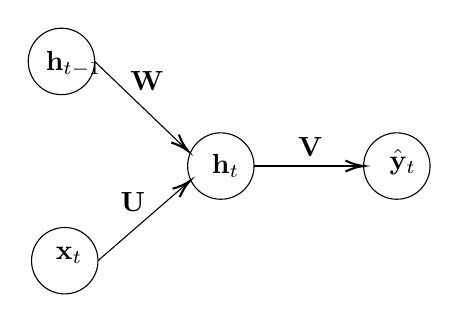
\begin{tikzpicture}[x=0.75pt,y=0.75pt,yscale=-0.8,xscale=0.8]
      %Shape: Ellipse [id:dp9795697082977448] 
      \draw   (412,88.33) .. controls (412,77.29) and (420.95,68.33) .. (432,68.33) .. controls (443.05,68.33) and (452,77.29) .. (452,88.33) .. controls (452,99.38) and (443.05,108.33) .. (432,108.33) .. controls (420.95,108.33) and (412,99.38) .. (412,88.33) -- cycle ;
      %Shape: Ellipse [id:dp8435868286837831] 
      \draw   (210,25.33) .. controls (210,14.29) and (218.95,5.33) .. (230,5.33) .. controls (241.05,5.33) and (250,14.29) .. (250,25.33) .. controls (250,36.38) and (241.05,45.33) .. (230,45.33) .. controls (218.95,45.33) and (210,36.38) .. (210,25.33) -- cycle ;
      %Shape: Ellipse [id:dp10562076709489165] 
      \draw   (306,88.33) .. controls (306,77.29) and (314.95,68.33) .. (326,68.33) .. controls (337.05,68.33) and (346,77.29) .. (346,88.33) .. controls (346,99.38) and (337.05,108.33) .. (326,108.33) .. controls (314.95,108.33) and (306,99.38) .. (306,88.33) -- cycle ;
      %Straight Lines [id:da00030920510583576366] 
      \draw [color={rgb, 255:red, 0; green, 0; blue, 0 }  ,draw opacity=1 ]   (250,25.33) -- (304.89,77.95) ;
      \draw [shift={(306.33,79.33)}, rotate = 223.79] [color={rgb, 255:red, 0; green, 0; blue, 0 }  ,draw opacity=1 ][line width=0.75]    (10.93,-3.29) .. controls (6.95,-1.4) and (3.31,-0.3) .. (0,0) .. controls (3.31,0.3) and (6.95,1.4) .. (10.93,3.29)   ;
      %Shape: Ellipse [id:dp611931387208084] 
      \draw   (212,145.33) .. controls (212,134.29) and (220.95,125.33) .. (232,125.33) .. controls (243.05,125.33) and (252,134.29) .. (252,145.33) .. controls (252,156.38) and (243.05,165.33) .. (232,165.33) .. controls (220.95,165.33) and (212,156.38) .. (212,145.33) -- cycle ;
      %Straight Lines [id:da04817982276379906] 
      \draw [color={rgb, 255:red, 0; green, 0; blue, 0 }  ,draw opacity=1 ]   (252,145.33) -- (305.82,98.64) ;
      \draw [shift={(307.33,97.33)}, rotate = 139.06] [color={rgb, 255:red, 0; green, 0; blue, 0 }  ,draw opacity=1 ][line width=0.75]    (10.93,-3.29) .. controls (6.95,-1.4) and (3.31,-0.3) .. (0,0) .. controls (3.31,0.3) and (6.95,1.4) .. (10.93,3.29)   ;
      %Straight Lines [id:da9431583172236413] 
      \draw [color={rgb, 255:red, 0; green, 0; blue, 0 }  ,draw opacity=1 ]   (346,88.33) -- (410,88.33) ;
      \draw [shift={(412,88.33)}, rotate = 180] [color={rgb, 255:red, 0; green, 0; blue, 0 }  ,draw opacity=1 ][line width=0.75]    (10.93,-3.29) .. controls (6.95,-1.4) and (3.31,-0.3) .. (0,0) .. controls (3.31,0.3) and (6.95,1.4) .. (10.93,3.29)   ;

      % Text Node
      \draw (219,17.73) node [anchor=north west][inner sep=0.75pt]  [font=\normalsize]  {$\mathbf{h}_{t-1}$};
      % Text Node
      \draw (319,79.73) node [anchor=north west][inner sep=0.75pt]  [font=\normalsize]  {$\mathbf{h}_{t}$};
      % Text Node
      \draw (270,29.73) node [anchor=north west][inner sep=0.75pt]  [font=\normalsize,color={rgb, 255:red, 0; green, 0; blue, 0 }  ,opacity=1 ]  {$\mathbf{W}$};
      % Text Node
      \draw (225,135.73) node [anchor=north west][inner sep=0.75pt]  [font=\normalsize]  {$\mathbf{x}_{t}$};
      % Text Node
      \draw (371,69.73) node [anchor=north west][inner sep=0.75pt]  [font=\normalsize,color={rgb, 255:red, 0; green, 0; blue, 0 }  ,opacity=1 ]  {$\mathbf{V}$};
      % Text Node
      \draw (264,102.73) node [anchor=north west][inner sep=0.75pt]  [font=\normalsize,color={rgb, 255:red, 0; green, 0; blue, 0 }  ,opacity=1 ]  {$\mathbf{U}$};
      % Text Node
      \draw (426,76.73) node [anchor=north west][inner sep=0.75pt]  [font=\normalsize]  {$\hat{\mathbf{y}}_{t}$};
    \end{tikzpicture}
    \caption{RNNs as an MLP. } 
    \label{fig:mlp_vs_rnn}
  \end{figure}

  \subsubsection{Loss Functions}

    The form of the loss for a RNN will have to be slightly modified, since we can have multiple outputs. If we have a given input-output pair $\mathbf{x}^{(n)}, \mathbf{y}^{(n)}$, and we are interested producing a single output, then this is similar to what we already do with regular NNs. If we are interested in producing a sequence of outputs, then we can average the loss functions individually so that equal weight is placed on the prediction at each relevant timestep. This is called 
    \begin{equation}
      L = \frac{1}{|T|} \sum_{t \in T} L_t
    \end{equation}
    Sometimes, even with single inputs it may be good to include other intermediate terms in the loss so that we can direct the neural net to converge faster to what the correct answer should be. 

    \begin{figure}[H]
      \centering 
      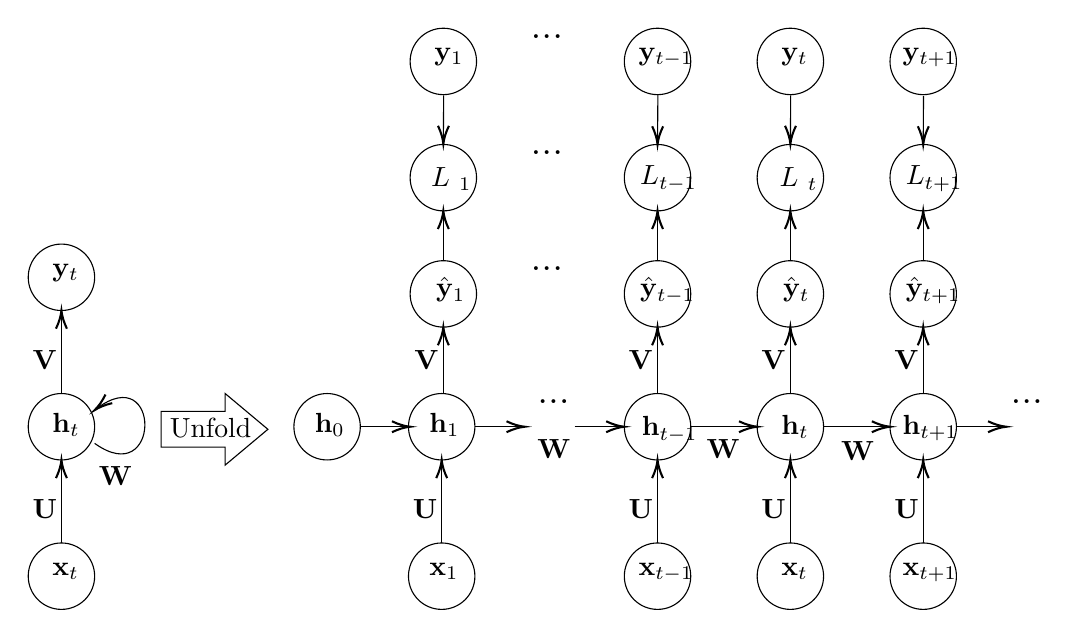
\begin{tikzpicture}[x=0.75pt,y=0.75pt,yscale=-0.8,xscale=0.8]
        %Shape: Ellipse [id:dp9680953270479153] 
        \draw   (30,160) .. controls (30,148.95) and (38.95,140) .. (50,140) .. controls (61.05,140) and (70,148.95) .. (70,160) .. controls (70,171.05) and (61.05,180) .. (50,180) .. controls (38.95,180) and (30,171.05) .. (30,160) -- cycle ;
        %Shape: Ellipse [id:dp5730005571966859] 
        \draw   (389,170) .. controls (389,158.95) and (397.95,150) .. (409,150) .. controls (420.05,150) and (429,158.95) .. (429,170) .. controls (429,181.05) and (420.05,190) .. (409,190) .. controls (397.95,190) and (389,181.05) .. (389,170) -- cycle ;
        %Shape: Ellipse [id:dp4570036898065337] 
        \draw   (549,170) .. controls (549,158.95) and (557.95,150) .. (569,150) .. controls (580.05,150) and (589,158.95) .. (589,170) .. controls (589,181.05) and (580.05,190) .. (569,190) .. controls (557.95,190) and (549,181.05) .. (549,170) -- cycle ;
        %Shape: Ellipse [id:dp310472974621425] 
        \draw   (469,170) .. controls (469,158.95) and (477.95,150) .. (489,150) .. controls (500.05,150) and (509,158.95) .. (509,170) .. controls (509,181.05) and (500.05,190) .. (489,190) .. controls (477.95,190) and (469,181.05) .. (469,170) -- cycle ;
        %Curve Lines [id:da9737186251466903] 
        \draw [color={rgb, 255:red, 0; green, 0; blue, 0 }  ,draw opacity=1 ]   (70,260) .. controls (109.93,288.71) and (110.33,209.61) .. (71.2,239.07) ;
        \draw [shift={(70,240)}, rotate = 321.57] [color={rgb, 255:red, 0; green, 0; blue, 0 }  ,draw opacity=1 ][line width=0.75]    (10.93,-3.29) .. controls (6.95,-1.4) and (3.31,-0.3) .. (0,0) .. controls (3.31,0.3) and (6.95,1.4) .. (10.93,3.29)   ;
        %Right Arrow [id:dp7863084495909953] 
        \draw   (110,240.77) -- (148.6,240.77) -- (148.6,230) -- (174.34,251.55) -- (148.6,273.1) -- (148.6,262.32) -- (110,262.32) -- cycle ;
        %Shape: Ellipse [id:dp6734347060174906] 
        \draw   (30,250) .. controls (30,238.95) and (38.95,230) .. (50,230) .. controls (61.05,230) and (70,238.95) .. (70,250) .. controls (70,261.05) and (61.05,270) .. (50,270) .. controls (38.95,270) and (30,261.05) .. (30,250) -- cycle ;
        %Shape: Ellipse [id:dp7555672305174788] 
        \draw   (389,250) .. controls (389,238.95) and (397.95,230) .. (409,230) .. controls (420.05,230) and (429,238.95) .. (429,250) .. controls (429,261.05) and (420.05,270) .. (409,270) .. controls (397.95,270) and (389,261.05) .. (389,250) -- cycle ;
        %Shape: Ellipse [id:dp8969160954412736] 
        \draw   (549,250) .. controls (549,238.95) and (557.95,230) .. (569,230) .. controls (580.05,230) and (589,238.95) .. (589,250) .. controls (589,261.05) and (580.05,270) .. (569,270) .. controls (557.95,270) and (549,261.05) .. (549,250) -- cycle ;
        %Shape: Ellipse [id:dp5010811857470736] 
        \draw   (469,250) .. controls (469,238.95) and (477.95,230) .. (489,230) .. controls (500.05,230) and (509,238.95) .. (509,250) .. controls (509,261.05) and (500.05,270) .. (489,270) .. controls (477.95,270) and (469,261.05) .. (469,250) -- cycle ;
        %Shape: Ellipse [id:dp15020874314124955] 
        \draw   (259,250) .. controls (259,238.95) and (267.95,230) .. (279,230) .. controls (290.05,230) and (299,238.95) .. (299,250) .. controls (299,261.05) and (290.05,270) .. (279,270) .. controls (267.95,270) and (259,261.05) .. (259,250) -- cycle ;
        %Straight Lines [id:da9739407532599313] 
        \draw [color={rgb, 255:red, 0; green, 0; blue, 0 }  ,draw opacity=1 ]   (299,250) -- (327,250) ;
        \draw [shift={(329,250)}, rotate = 180] [color={rgb, 255:red, 0; green, 0; blue, 0 }  ,draw opacity=1 ][line width=0.75]    (10.93,-3.29) .. controls (6.95,-1.4) and (3.31,-0.3) .. (0,0) .. controls (3.31,0.3) and (6.95,1.4) .. (10.93,3.29)   ;
        %Straight Lines [id:da42172683153715984] 
        \draw [color={rgb, 255:red, 0; green, 0; blue, 0 }  ,draw opacity=1 ]   (359,250) -- (387,250) ;
        \draw [shift={(389,250)}, rotate = 180] [color={rgb, 255:red, 0; green, 0; blue, 0 }  ,draw opacity=1 ][line width=0.75]    (10.93,-3.29) .. controls (6.95,-1.4) and (3.31,-0.3) .. (0,0) .. controls (3.31,0.3) and (6.95,1.4) .. (10.93,3.29)   ;
        %Straight Lines [id:da6928721729158405] 
        \draw [color={rgb, 255:red, 0; green, 0; blue, 0 }  ,draw opacity=1 ]   (429,250) -- (467,250) ;
        \draw [shift={(469,250)}, rotate = 180] [color={rgb, 255:red, 0; green, 0; blue, 0 }  ,draw opacity=1 ][line width=0.75]    (10.93,-3.29) .. controls (6.95,-1.4) and (3.31,-0.3) .. (0,0) .. controls (3.31,0.3) and (6.95,1.4) .. (10.93,3.29)   ;
        %Straight Lines [id:da9699219090048701] 
        \draw [color={rgb, 255:red, 0; green, 0; blue, 0 }  ,draw opacity=1 ]   (509,250) -- (547,250) ;
        \draw [shift={(549,250)}, rotate = 180] [color={rgb, 255:red, 0; green, 0; blue, 0 }  ,draw opacity=1 ][line width=0.75]    (10.93,-3.29) .. controls (6.95,-1.4) and (3.31,-0.3) .. (0,0) .. controls (3.31,0.3) and (6.95,1.4) .. (10.93,3.29)   ;
        %Straight Lines [id:da9089120498679435] 
        \draw [color={rgb, 255:red, 0; green, 0; blue, 0 }  ,draw opacity=1 ]   (589,250) -- (617,250) ;
        \draw [shift={(619,250)}, rotate = 180] [color={rgb, 255:red, 0; green, 0; blue, 0 }  ,draw opacity=1 ][line width=0.75]    (10.93,-3.29) .. controls (6.95,-1.4) and (3.31,-0.3) .. (0,0) .. controls (3.31,0.3) and (6.95,1.4) .. (10.93,3.29)   ;
        %Shape: Ellipse [id:dp2664716169413004] 
        \draw   (30,340) .. controls (30,328.95) and (38.95,320) .. (50,320) .. controls (61.05,320) and (70,328.95) .. (70,340) .. controls (70,351.05) and (61.05,360) .. (50,360) .. controls (38.95,360) and (30,351.05) .. (30,340) -- cycle ;
        %Shape: Ellipse [id:dp9588931299107948] 
        \draw   (389,340) .. controls (389,328.95) and (397.95,320) .. (409,320) .. controls (420.05,320) and (429,328.95) .. (429,340) .. controls (429,351.05) and (420.05,360) .. (409,360) .. controls (397.95,360) and (389,351.05) .. (389,340) -- cycle ;
        %Shape: Ellipse [id:dp011971914379850457] 
        \draw   (549,340) .. controls (549,328.95) and (557.95,320) .. (569,320) .. controls (580.05,320) and (589,328.95) .. (589,340) .. controls (589,351.05) and (580.05,360) .. (569,360) .. controls (557.95,360) and (549,351.05) .. (549,340) -- cycle ;
        %Shape: Ellipse [id:dp9234187724355627] 
        \draw   (469,340) .. controls (469,328.95) and (477.95,320) .. (489,320) .. controls (500.05,320) and (509,328.95) .. (509,340) .. controls (509,351.05) and (500.05,360) .. (489,360) .. controls (477.95,360) and (469,351.05) .. (469,340) -- cycle ;
        %Shape: Ellipse [id:dp32361468564640217] 
        \draw   (259,340) .. controls (259,328.95) and (267.95,320) .. (279,320) .. controls (290.05,320) and (299,328.95) .. (299,340) .. controls (299,351.05) and (290.05,360) .. (279,360) .. controls (267.95,360) and (259,351.05) .. (259,340) -- cycle ;
        %Straight Lines [id:da17794535301053505] 
        \draw [color={rgb, 255:red, 0; green, 0; blue, 0 }  ,draw opacity=1 ]   (279,320) -- (279,272) ;
        \draw [shift={(279,270)}, rotate = 90] [color={rgb, 255:red, 0; green, 0; blue, 0 }  ,draw opacity=1 ][line width=0.75]    (10.93,-3.29) .. controls (6.95,-1.4) and (3.31,-0.3) .. (0,0) .. controls (3.31,0.3) and (6.95,1.4) .. (10.93,3.29)   ;
        %Straight Lines [id:da39434249393019916] 
        \draw [color={rgb, 255:red, 0; green, 0; blue, 0 }  ,draw opacity=1 ]   (409,230) -- (409,192) ;
        \draw [shift={(409,190)}, rotate = 90] [color={rgb, 255:red, 0; green, 0; blue, 0 }  ,draw opacity=1 ][line width=0.75]    (10.93,-3.29) .. controls (6.95,-1.4) and (3.31,-0.3) .. (0,0) .. controls (3.31,0.3) and (6.95,1.4) .. (10.93,3.29)   ;
        %Straight Lines [id:da8293325821143183] 
        \draw [color={rgb, 255:red, 0; green, 0; blue, 0 }  ,draw opacity=1 ]   (409,320) -- (409,272) ;
        \draw [shift={(409,270)}, rotate = 90] [color={rgb, 255:red, 0; green, 0; blue, 0 }  ,draw opacity=1 ][line width=0.75]    (10.93,-3.29) .. controls (6.95,-1.4) and (3.31,-0.3) .. (0,0) .. controls (3.31,0.3) and (6.95,1.4) .. (10.93,3.29)   ;
        %Straight Lines [id:da22535194171078898] 
        \draw [color={rgb, 255:red, 0; green, 0; blue, 0 }  ,draw opacity=1 ]   (489,230) -- (489,196) -- (489,192) ;
        \draw [shift={(489,190)}, rotate = 90] [color={rgb, 255:red, 0; green, 0; blue, 0 }  ,draw opacity=1 ][line width=0.75]    (10.93,-3.29) .. controls (6.95,-1.4) and (3.31,-0.3) .. (0,0) .. controls (3.31,0.3) and (6.95,1.4) .. (10.93,3.29)   ;
        %Straight Lines [id:da22035114948288692] 
        \draw [color={rgb, 255:red, 0; green, 0; blue, 0 }  ,draw opacity=1 ]   (489,320) -- (489,272) ;
        \draw [shift={(489,270)}, rotate = 90] [color={rgb, 255:red, 0; green, 0; blue, 0 }  ,draw opacity=1 ][line width=0.75]    (10.93,-3.29) .. controls (6.95,-1.4) and (3.31,-0.3) .. (0,0) .. controls (3.31,0.3) and (6.95,1.4) .. (10.93,3.29)   ;
        %Straight Lines [id:da4608028249993794] 
        \draw [color={rgb, 255:red, 0; green, 0; blue, 0 }  ,draw opacity=1 ]   (569,230) -- (569,192) ;
        \draw [shift={(569,190)}, rotate = 90] [color={rgb, 255:red, 0; green, 0; blue, 0 }  ,draw opacity=1 ][line width=0.75]    (10.93,-3.29) .. controls (6.95,-1.4) and (3.31,-0.3) .. (0,0) .. controls (3.31,0.3) and (6.95,1.4) .. (10.93,3.29)   ;
        %Straight Lines [id:da1823633965200031] 
        \draw [color={rgb, 255:red, 0; green, 0; blue, 0 }  ,draw opacity=1 ]   (569,320) -- (569,272) ;
        \draw [shift={(569,270)}, rotate = 90] [color={rgb, 255:red, 0; green, 0; blue, 0 }  ,draw opacity=1 ][line width=0.75]    (10.93,-3.29) .. controls (6.95,-1.4) and (3.31,-0.3) .. (0,0) .. controls (3.31,0.3) and (6.95,1.4) .. (10.93,3.29)   ;
        %Straight Lines [id:da8056932056306494] 
        \draw [color={rgb, 255:red, 0; green, 0; blue, 0 }  ,draw opacity=1 ]   (50,230) -- (50,182) ;
        \draw [shift={(50,180)}, rotate = 90] [color={rgb, 255:red, 0; green, 0; blue, 0 }  ,draw opacity=1 ][line width=0.75]    (10.93,-3.29) .. controls (6.95,-1.4) and (3.31,-0.3) .. (0,0) .. controls (3.31,0.3) and (6.95,1.4) .. (10.93,3.29)   ;
        %Straight Lines [id:da36005109179707473] 
        \draw [color={rgb, 255:red, 0; green, 0; blue, 0 }  ,draw opacity=1 ]   (50,320) -- (50,272) ;
        \draw [shift={(50,270)}, rotate = 90] [color={rgb, 255:red, 0; green, 0; blue, 0 }  ,draw opacity=1 ][line width=0.75]    (10.93,-3.29) .. controls (6.95,-1.4) and (3.31,-0.3) .. (0,0) .. controls (3.31,0.3) and (6.95,1.4) .. (10.93,3.29)   ;
        %Shape: Ellipse [id:dp7699860556623466] 
        \draw   (389,30) .. controls (389,18.95) and (397.95,10) .. (409,10) .. controls (420.05,10) and (429,18.95) .. (429,30) .. controls (429,41.05) and (420.05,50) .. (409,50) .. controls (397.95,50) and (389,41.05) .. (389,30) -- cycle ;
        %Shape: Ellipse [id:dp8781760286661879] 
        \draw   (549,30) .. controls (549,18.95) and (557.95,10) .. (569,10) .. controls (580.05,10) and (589,18.95) .. (589,30) .. controls (589,41.05) and (580.05,50) .. (569,50) .. controls (557.95,50) and (549,41.05) .. (549,30) -- cycle ;
        %Shape: Ellipse [id:dp8200489227369978] 
        \draw   (469,30) .. controls (469,18.95) and (477.95,10) .. (489,10) .. controls (500.05,10) and (509,18.95) .. (509,30) .. controls (509,41.05) and (500.05,50) .. (489,50) .. controls (477.95,50) and (469,41.05) .. (469,30) -- cycle ;
        %Straight Lines [id:da9146271026162445] 
        \draw [color={rgb, 255:red, 0; green, 0; blue, 0 }  ,draw opacity=1 ]   (409,150) -- (409,122) ;
        \draw [shift={(409,120)}, rotate = 90] [color={rgb, 255:red, 0; green, 0; blue, 0 }  ,draw opacity=1 ][line width=0.75]    (10.93,-3.29) .. controls (6.95,-1.4) and (3.31,-0.3) .. (0,0) .. controls (3.31,0.3) and (6.95,1.4) .. (10.93,3.29)   ;
        %Straight Lines [id:da5910213404038462] 
        \draw [color={rgb, 255:red, 0; green, 0; blue, 0 }  ,draw opacity=1 ]   (489,150) -- (489,124.5) -- (489,122) ;
        \draw [shift={(489,120)}, rotate = 90] [color={rgb, 255:red, 0; green, 0; blue, 0 }  ,draw opacity=1 ][line width=0.75]    (10.93,-3.29) .. controls (6.95,-1.4) and (3.31,-0.3) .. (0,0) .. controls (3.31,0.3) and (6.95,1.4) .. (10.93,3.29)   ;
        %Straight Lines [id:da8117346403410379] 
        \draw [color={rgb, 255:red, 0; green, 0; blue, 0 }  ,draw opacity=1 ]   (569,150) -- (569,122) ;
        \draw [shift={(569,120)}, rotate = 90] [color={rgb, 255:red, 0; green, 0; blue, 0 }  ,draw opacity=1 ][line width=0.75]    (10.93,-3.29) .. controls (6.95,-1.4) and (3.31,-0.3) .. (0,0) .. controls (3.31,0.3) and (6.95,1.4) .. (10.93,3.29)   ;
        %Straight Lines [id:da7693558246165639] 
        \draw [color={rgb, 255:red, 0; green, 0; blue, 0 }  ,draw opacity=1 ]   (569.19,50.68) -- (569.01,78) ;
        \draw [shift={(569,80)}, rotate = 270.38] [color={rgb, 255:red, 0; green, 0; blue, 0 }  ,draw opacity=1 ][line width=0.75]    (10.93,-3.29) .. controls (6.95,-1.4) and (3.31,-0.3) .. (0,0) .. controls (3.31,0.3) and (6.95,1.4) .. (10.93,3.29)   ;
        %Straight Lines [id:da0885606332920994] 
        \draw [color={rgb, 255:red, 0; green, 0; blue, 0 }  ,draw opacity=1 ]   (489.19,50.39) -- (489.03,75.32) -- (489.01,77.71) ;
        \draw [shift={(489,79.71)}, rotate = 270.38] [color={rgb, 255:red, 0; green, 0; blue, 0 }  ,draw opacity=1 ][line width=0.75]    (10.93,-3.29) .. controls (6.95,-1.4) and (3.31,-0.3) .. (0,0) .. controls (3.31,0.3) and (6.95,1.4) .. (10.93,3.29)   ;
        %Straight Lines [id:da8093446483541116] 
        \draw [color={rgb, 255:red, 0; green, 0; blue, 0 }  ,draw opacity=1 ]   (409.2,50) -- (409.01,78) ;
        \draw [shift={(409,80)}, rotate = 270.37] [color={rgb, 255:red, 0; green, 0; blue, 0 }  ,draw opacity=1 ][line width=0.75]    (10.93,-3.29) .. controls (6.95,-1.4) and (3.31,-0.3) .. (0,0) .. controls (3.31,0.3) and (6.95,1.4) .. (10.93,3.29)   ;
        %Shape: Ellipse [id:dp3418522481404773] 
        \draw   (389,100) .. controls (389,88.95) and (397.95,80) .. (409,80) .. controls (420.05,80) and (429,88.95) .. (429,100) .. controls (429,111.05) and (420.05,120) .. (409,120) .. controls (397.95,120) and (389,111.05) .. (389,100) -- cycle ;
        %Shape: Ellipse [id:dp06970312979796955] 
        \draw   (549,100) .. controls (549,88.95) and (557.95,80) .. (569,80) .. controls (580.05,80) and (589,88.95) .. (589,100) .. controls (589,111.05) and (580.05,120) .. (569,120) .. controls (557.95,120) and (549,111.05) .. (549,100) -- cycle ;
        %Shape: Ellipse [id:dp9790373728494837] 
        \draw   (469,100) .. controls (469,88.95) and (477.95,80) .. (489,80) .. controls (500.05,80) and (509,88.95) .. (509,100) .. controls (509,111.05) and (500.05,120) .. (489,120) .. controls (477.95,120) and (469,111.05) .. (469,100) -- cycle ;
        %Shape: Ellipse [id:dp37862988101859396] 
        \draw   (190,250) .. controls (190,238.95) and (198.95,230) .. (210,230) .. controls (221.05,230) and (230,238.95) .. (230,250) .. controls (230,261.05) and (221.05,270) .. (210,270) .. controls (198.95,270) and (190,261.05) .. (190,250) -- cycle ;
        %Straight Lines [id:da4404897581281486] 
        \draw [color={rgb, 255:red, 0; green, 0; blue, 0 }  ,draw opacity=1 ]   (230,250) -- (258,250) ;
        \draw [shift={(260,250)}, rotate = 180] [color={rgb, 255:red, 0; green, 0; blue, 0 }  ,draw opacity=1 ][line width=0.75]    (10.93,-3.29) .. controls (6.95,-1.4) and (3.31,-0.3) .. (0,0) .. controls (3.31,0.3) and (6.95,1.4) .. (10.93,3.29)   ;
        %Shape: Ellipse [id:dp9704314855218612] 
        \draw   (260,170) .. controls (260,158.95) and (268.95,150) .. (280,150) .. controls (291.05,150) and (300,158.95) .. (300,170) .. controls (300,181.05) and (291.05,190) .. (280,190) .. controls (268.95,190) and (260,181.05) .. (260,170) -- cycle ;
        %Straight Lines [id:da33577641284261595] 
        \draw [color={rgb, 255:red, 0; green, 0; blue, 0 }  ,draw opacity=1 ]   (280,230) -- (280,196) -- (280,192) ;
        \draw [shift={(280,190)}, rotate = 90] [color={rgb, 255:red, 0; green, 0; blue, 0 }  ,draw opacity=1 ][line width=0.75]    (10.93,-3.29) .. controls (6.95,-1.4) and (3.31,-0.3) .. (0,0) .. controls (3.31,0.3) and (6.95,1.4) .. (10.93,3.29)   ;
        %Shape: Ellipse [id:dp1313244139349521] 
        \draw   (260,30) .. controls (260,18.95) and (268.95,10) .. (280,10) .. controls (291.05,10) and (300,18.95) .. (300,30) .. controls (300,41.05) and (291.05,50) .. (280,50) .. controls (268.95,50) and (260,41.05) .. (260,30) -- cycle ;
        %Straight Lines [id:da00658706292138822] 
        \draw [color={rgb, 255:red, 0; green, 0; blue, 0 }  ,draw opacity=1 ]   (280,150) -- (280,124.5) -- (280,122) ;
        \draw [shift={(280,120)}, rotate = 90] [color={rgb, 255:red, 0; green, 0; blue, 0 }  ,draw opacity=1 ][line width=0.75]    (10.93,-3.29) .. controls (6.95,-1.4) and (3.31,-0.3) .. (0,0) .. controls (3.31,0.3) and (6.95,1.4) .. (10.93,3.29)   ;
        %Straight Lines [id:da9543130195161293] 
        \draw [color={rgb, 255:red, 0; green, 0; blue, 0 }  ,draw opacity=1 ]   (280.19,50.39) -- (280.03,75.32) -- (280.01,77.71) ;
        \draw [shift={(280,79.71)}, rotate = 270.38] [color={rgb, 255:red, 0; green, 0; blue, 0 }  ,draw opacity=1 ][line width=0.75]    (10.93,-3.29) .. controls (6.95,-1.4) and (3.31,-0.3) .. (0,0) .. controls (3.31,0.3) and (6.95,1.4) .. (10.93,3.29)   ;
        %Shape: Ellipse [id:dp6237018603296542] 
        \draw   (260,100) .. controls (260,88.95) and (268.95,80) .. (280,80) .. controls (291.05,80) and (300,88.95) .. (300,100) .. controls (300,111.05) and (291.05,120) .. (280,120) .. controls (268.95,120) and (260,111.05) .. (260,100) -- cycle ;

        % Text Node
        \draw (335,232) node [anchor=north west][inner sep=0.75pt]  [font=\Large] [align=left] {...};
        % Text Node
        \draw (397,158.4) node [anchor=north west][inner sep=0.75pt]  [font=\normalsize]  {$\hat{\mathbf{y}}_{t-1}$};
        % Text Node
        \draw (113.69,243.09) node [anchor=north west][inner sep=0.75pt]   [align=left] {Unfold};
        % Text Node
        \draw (335,256.4) node [anchor=north west][inner sep=0.75pt]  [font=\normalsize,color={rgb, 255:red, 0; green, 0; blue, 0 }  ,opacity=1 ]  {$\mathbf{W}$};
        % Text Node
        \draw (43,150.4) node [anchor=north west][inner sep=0.75pt]  [font=\normalsize]  {$\mathbf{y}_{t}$};
        % Text Node
        \draw (270,240.4) node [anchor=north west][inner sep=0.75pt]  [font=\normalsize]  {$\mathbf{h}_{1}$};
        % Text Node
        \draw (398,242.4) node [anchor=north west][inner sep=0.75pt]  [font=\normalsize]  {$\mathbf{h}_{t-1}$};
        % Text Node
        \draw (482,241.4) node [anchor=north west][inner sep=0.75pt]  [font=\normalsize]  {$\mathbf{h}_{t}$};
        % Text Node
        \draw (555,241.4) node [anchor=north west][inner sep=0.75pt]  [font=\normalsize]  {$\mathbf{h}_{t+1}$};
        % Text Node
        \draw (43,240.4) node [anchor=north west][inner sep=0.75pt]  [font=\normalsize]  {$\mathbf{h}_{t}$};
        % Text Node
        \draw (620,232) node [anchor=north west][inner sep=0.75pt]  [font=\Large] [align=left] {...};
        % Text Node
        \draw (437,256.4) node [anchor=north west][inner sep=0.75pt]  [font=\normalsize,color={rgb, 255:red, 0; green, 0; blue, 0 }  ,opacity=1 ]  {$\mathbf{W}$};
        % Text Node
        \draw (270,330.4) node [anchor=north west][inner sep=0.75pt]  [font=\normalsize]  {$\mathbf{x}_{1}$};
        % Text Node
        \draw (396,330.4) node [anchor=north west][inner sep=0.75pt]  [font=\normalsize]  {$\mathbf{x}_{t-1}$};
        % Text Node
        \draw (482,330.4) node [anchor=north west][inner sep=0.75pt]  [font=\normalsize]  {$\mathbf{x}_{t}$};
        % Text Node
        \draw (555,330.4) node [anchor=north west][inner sep=0.75pt]  [font=\normalsize]  {$\mathbf{x}_{t+1}$};
        % Text Node
        \draw (43,330.4) node [anchor=north west][inner sep=0.75pt]  [font=\normalsize]  {$\mathbf{x}_{t}$};
        % Text Node
        \draw (260,292.4) node [anchor=north west][inner sep=0.75pt]  [font=\normalsize,color={rgb, 255:red, 0; green, 0; blue, 0 }  ,opacity=1 ]  {$\mathbf{U}$};
        % Text Node
        \draw (71,272.4) node [anchor=north west][inner sep=0.75pt]  [font=\normalsize,color={rgb, 255:red, 0; green, 0; blue, 0 }  ,opacity=1 ]  {$\mathbf{W}$};
        % Text Node
        \draw (390,202.4) node [anchor=north west][inner sep=0.75pt]  [font=\normalsize,color={rgb, 255:red, 0; green, 0; blue, 0 }  ,opacity=1 ]  {$\mathbf{V}$};
        % Text Node
        \draw (390,292.4) node [anchor=north west][inner sep=0.75pt]  [font=\normalsize,color={rgb, 255:red, 0; green, 0; blue, 0 }  ,opacity=1 ]  {$\mathbf{U}$};
        % Text Node
        \draw (470,202.4) node [anchor=north west][inner sep=0.75pt]  [font=\normalsize,color={rgb, 255:red, 0; green, 0; blue, 0 }  ,opacity=1 ]  {$\mathbf{V}$};
        % Text Node
        \draw (470,292.4) node [anchor=north west][inner sep=0.75pt]  [font=\normalsize,color={rgb, 255:red, 0; green, 0; blue, 0 }  ,opacity=1 ]  {$\mathbf{U}$};
        % Text Node
        \draw (550,202.4) node [anchor=north west][inner sep=0.75pt]  [font=\normalsize,color={rgb, 255:red, 0; green, 0; blue, 0 }  ,opacity=1 ]  {$\mathbf{V}$};
        % Text Node
        \draw (550,292.4) node [anchor=north west][inner sep=0.75pt]  [font=\normalsize,color={rgb, 255:red, 0; green, 0; blue, 0 }  ,opacity=1 ]  {$\mathbf{U}$};
        % Text Node
        \draw (31,202.4) node [anchor=north west][inner sep=0.75pt]  [font=\normalsize,color={rgb, 255:red, 0; green, 0; blue, 0 }  ,opacity=1 ]  {$\mathbf{V}$};
        % Text Node
        \draw (31,292.4) node [anchor=north west][inner sep=0.75pt]  [font=\normalsize,color={rgb, 255:red, 0; green, 0; blue, 0 }  ,opacity=1 ]  {$\mathbf{U}$};
        % Text Node
        \draw (518,257.4) node [anchor=north west][inner sep=0.75pt]  [font=\normalsize,color={rgb, 255:red, 0; green, 0; blue, 0 }  ,opacity=1 ]  {$\mathbf{W}$};
        % Text Node
        \draw (483,158.4) node [anchor=north west][inner sep=0.75pt]  [font=\normalsize]  {$\hat{\mathbf{y}}_{t}$};
        % Text Node
        \draw (557,158.4) node [anchor=north west][inner sep=0.75pt]  [font=\normalsize]  {$\hat{\mathbf{y}}_{t+1}$};
        % Text Node
        \draw (396,20.4) node [anchor=north west][inner sep=0.75pt]  [font=\normalsize]  {$\mathbf{y}_{t-1}$};
        % Text Node
        \draw (482,20.4) node [anchor=north west][inner sep=0.75pt]  [font=\normalsize]  {$\mathbf{y}_{t}$};
        % Text Node
        \draw (555,20.4) node [anchor=north west][inner sep=0.75pt]  [font=\normalsize]  {$\mathbf{y}_{t+1}$};
        % Text Node
        \draw (397,91.4) node [anchor=north west][inner sep=0.75pt]  [font=\normalsize]  {$L_{t-1}$};
        % Text Node
        \draw (481,92.4) node [anchor=north west][inner sep=0.75pt]  [font=\normalsize]  {$L_{\ t}$};
        % Text Node
        \draw (557,91.4) node [anchor=north west][inner sep=0.75pt]  [font=\normalsize]  {$L_{t+1}$};
        % Text Node
        \draw (201,240.4) node [anchor=north west][inner sep=0.75pt]  [font=\normalsize]  {$\mathbf{h}_{0}$};
        % Text Node
        \draw (261,202.4) node [anchor=north west][inner sep=0.75pt]  [font=\normalsize,color={rgb, 255:red, 0; green, 0; blue, 0 }  ,opacity=1 ]  {$\mathbf{V}$};
        % Text Node
        \draw (274,158.4) node [anchor=north west][inner sep=0.75pt]  [font=\normalsize]  {$\hat{\mathbf{y}}_{1}$};
        % Text Node
        \draw (273,20.4) node [anchor=north west][inner sep=0.75pt]  [font=\normalsize]  {$\mathbf{y}_{1}$};
        % Text Node
        \draw (271,92.4) node [anchor=north west][inner sep=0.75pt]  [font=\normalsize]  {$L_{\ 1}$};
        % Text Node
        \draw (331,152) node [anchor=north west][inner sep=0.75pt]  [font=\Large] [align=left] {...};
        % Text Node
        \draw (331,82) node [anchor=north west][inner sep=0.75pt]  [font=\Large] [align=left] {...};
        % Text Node
        \draw (331,12) node [anchor=north west][inner sep=0.75pt]  [font=\Large] [align=left] {...};
      \end{tikzpicture}
      \caption{} 
      \label{fig:rnn_w_loss}
    \end{figure}

    Note that one problem is that the errors can build up as the RNN predicts outcomes. For example, if we predicted $\mathbf{x}_1 \mapsto \hat{\mathbf{y}}_1$ we can compute the loss as $L_1 (\mathbf{y}_1, \hat{\mathbf{y}}_1)$. However, there are two ways to compute the second loss: with inputs $L_2 (\mathbf{x}_1, \mathbf{x}_2)$ or with $L_2 (\mathbf{x}_1, \hat{\mathbf{y}}_1)$. One just uses the ground truth while the other uses the previous prediction for the next prediction, which can accumulate error. Both ways are feasible for loss computation, but it is generally done in the former way, called \textbf{teacher forcing}. This is analogous to a human student taking a multi-part exam where the answer to each part depends on the answer to the preceding part. Rather than grading every answer in the end, with the risk that the student fails every single part even though they only made a mistake in the first one, a teacher records the score for each individual part and then tells the student the correct answer, to be used in the next part. 

  \subsubsection{Backpropagation Through Time}

    Now if we wanted to backpropagate through this RNN, we can compute 
    \begin{equation}
      \frac{\partial L_t}{\partial \mathbf{W}} = \frac{\partial L_t}{\partial \hat{\mathbf{y}}_t} \, \frac{\partial \hat{\mathbf{y}}_t}{\partial \mathbf{h}_t} \, \frac{\partial \mathbf{h}_t}{\partial \mathbf{W}}
    \end{equation}
    where the first term depends on the specific form of the loss and the second is simply the matrix $\mathbf{V}$. This all looks the same as backpropagation for a MLP, but since $\mathbf{W}_{hh}$ is used at multiple layers, we can reduce the third term in the equation to 
    \begin{equation}
      \frac{\partial L_t}{\partial \mathbf{W}} = \frac{\partial L_t}{\partial \hat{\mathbf{y}}_t} \, \frac{\partial \hat{\mathbf{y}}_t}{\partial \mathbf{h}_t} \, \bigg(\sum_{k=1}^t \frac{\partial \mathbf{h}_t}{\partial \mathbf{h}_k} \, \frac{\partial \mathbf{h}_k}{\partial \mathbf{W}} \bigg)
    \end{equation}
    where 
    \begin{equation}
      \frac{\partial \mathbf{h}_t}{\partial \mathbf{h}_k}  = \prod_{i=k+1}^{t} \frac{\partial \mathbf{h}_i}{\partial \mathbf{h}_{i-1}}
    \end{equation}
    is computed as a multiplication of adjacent time steps. Now this can be very problematic, since if we have a lot of multiplications, then depending on the randomness of these matrices the gradient may be highly unstable, causing the vanishing or exploding gradient problem. We can elaborate on this a little further. Note that the hidden linear maps are known to be square matrices. We can expand out the derivative without the constant terms on the left as such: 
    \begin{equation}
      \sum_{k=1}^t \frac{\partial \mathbf{h}_t}{\partial \mathbf{h}_k} \, \frac{\partial \mathbf{h}_k}{\partial \mathbf{W}} = \sum_{k=1}^t \prod_{k < i \leq t} \frac{\partial \mathbf{h}_i}{\partial \mathbf{h}_{i-1}} \; \frac{\partial \mathbf{h}_k}{\partial \mathbf{W}}
    \end{equation}
    and we can see if at some point one of the $\frac{\partial \mathbf{h}_j}{\partial \mathbf{h}_{j-1}}$ tend to be small just from randomness, then their product for all coefficients where $k \leq j$ will be small too. This means that all the information, or memory, from the $j$th hidden state and before will vanish. In fact, if the spectrum (the set of eigenvalues and eigenvectors) is less than $1$, then the multiplication of these derivatives will converge to a $0$ matrix, and so we have an exponential memory loss throughout the network. 

    Furthermore, we can compute these gradients in batches by splitting up the corpus into several sentences, and sampling the sentences for gradient computation. Therefore, a forward or backward pass has a runtime complexity of $O(\tau)$ and cannot be reduced by parallelization because the forward propagation graph is inherently sequential. Each time step may only be computed after the previous one. States computed in the forward pass must be stored until they are reused during the backward pass, so the memory cost is also $O(\tau)$. 

  \subsubsection{Stacked Unidirectional RNNs}

    Note that since we really have three matrices to optimize in the regular RNN, this may not be so robust. Therefore, we would like more hidden layers to capture further nonlinearities in an RNN, which is why we introduce a \textbf{stacked RNN} as shown below: 

    \begin{figure}[H]
      \centering 
      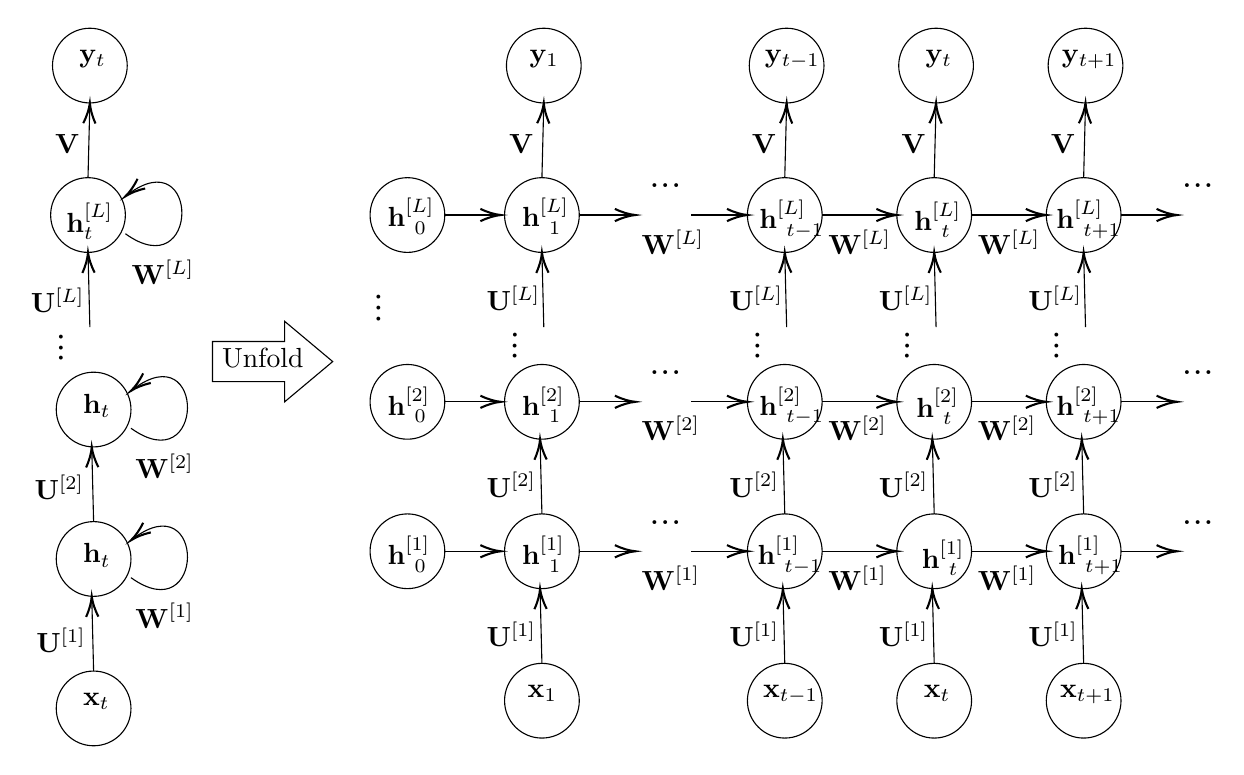
\begin{tikzpicture}[x=0.75pt,y=0.75pt,yscale=-0.9,xscale=0.9]
        %Shape: Ellipse [id:dp28408170140830746] 
        \draw   (24,35.87) .. controls (24,24.82) and (32.95,15.87) .. (44,15.87) .. controls (55.05,15.87) and (64,24.82) .. (64,35.87) .. controls (64,46.91) and (55.05,55.87) .. (44,55.87) .. controls (32.95,55.87) and (24,46.91) .. (24,35.87) -- cycle ;
        %Shape: Ellipse [id:dp8781268953519794] 
        \draw   (397,35.87) .. controls (397,24.82) and (405.95,15.87) .. (417,15.87) .. controls (428.05,15.87) and (437,24.82) .. (437,35.87) .. controls (437,46.91) and (428.05,55.87) .. (417,55.87) .. controls (405.95,55.87) and (397,46.91) .. (397,35.87) -- cycle ;
        %Shape: Ellipse [id:dp23070246888253831] 
        \draw   (557,35.87) .. controls (557,24.82) and (565.95,15.87) .. (577,15.87) .. controls (588.05,15.87) and (597,24.82) .. (597,35.87) .. controls (597,46.91) and (588.05,55.87) .. (577,55.87) .. controls (565.95,55.87) and (557,46.91) .. (557,35.87) -- cycle ;
        %Shape: Ellipse [id:dp8813319478015851] 
        \draw   (477,35.87) .. controls (477,24.82) and (485.95,15.87) .. (497,15.87) .. controls (508.05,15.87) and (517,24.82) .. (517,35.87) .. controls (517,46.91) and (508.05,55.87) .. (497,55.87) .. controls (485.95,55.87) and (477,46.91) .. (477,35.87) -- cycle ;
        %Shape: Ellipse [id:dp8173412138940122] 
        \draw   (267,35.87) .. controls (267,24.82) and (275.95,15.87) .. (287,15.87) .. controls (298.05,15.87) and (307,24.82) .. (307,35.87) .. controls (307,46.91) and (298.05,55.87) .. (287,55.87) .. controls (275.95,55.87) and (267,46.91) .. (267,35.87) -- cycle ;
        %Curve Lines [id:da5852340038150265] 
        \draw [color={rgb, 255:red, 0; green, 0; blue, 0 }  ,draw opacity=1 ]   (63,125.87) .. controls (102.93,154.58) and (103.33,75.48) .. (64.2,104.94) ;
        \draw [shift={(63,105.87)}, rotate = 321.57] [color={rgb, 255:red, 0; green, 0; blue, 0 }  ,draw opacity=1 ][line width=0.75]    (10.93,-3.29) .. controls (6.95,-1.4) and (3.31,-0.3) .. (0,0) .. controls (3.31,0.3) and (6.95,1.4) .. (10.93,3.29)   ;
        %Right Arrow [id:dp9792060545910206] 
        \draw   (109.66,183.55) -- (148.27,183.55) -- (148.27,172.77) -- (174,194.32) -- (148.27,215.87) -- (148.27,205.09) -- (109.66,205.09) -- cycle ;
        %Straight Lines [id:da04658286485976837] 
        \draw [color={rgb, 255:red, 0; green, 0; blue, 0 }  ,draw opacity=1 ]   (286,95.87) -- (286.95,57.87) ;
        \draw [shift={(287,55.87)}, rotate = 91.43] [color={rgb, 255:red, 0; green, 0; blue, 0 }  ,draw opacity=1 ][line width=0.75]    (10.93,-3.29) .. controls (6.95,-1.4) and (3.31,-0.3) .. (0,0) .. controls (3.31,0.3) and (6.95,1.4) .. (10.93,3.29)   ;
        %Shape: Ellipse [id:dp6328894287664162] 
        \draw   (23,115.87) .. controls (23,104.82) and (31.95,95.87) .. (43,95.87) .. controls (54.05,95.87) and (63,104.82) .. (63,115.87) .. controls (63,126.91) and (54.05,135.87) .. (43,135.87) .. controls (31.95,135.87) and (23,126.91) .. (23,115.87) -- cycle ;
        %Shape: Ellipse [id:dp25191747098174755] 
        \draw   (396,115.87) .. controls (396,104.82) and (404.95,95.87) .. (416,95.87) .. controls (427.05,95.87) and (436,104.82) .. (436,115.87) .. controls (436,126.91) and (427.05,135.87) .. (416,135.87) .. controls (404.95,135.87) and (396,126.91) .. (396,115.87) -- cycle ;
        %Shape: Ellipse [id:dp006489502181648232] 
        \draw   (556,115.87) .. controls (556,104.82) and (564.95,95.87) .. (576,95.87) .. controls (587.05,95.87) and (596,104.82) .. (596,115.87) .. controls (596,126.91) and (587.05,135.87) .. (576,135.87) .. controls (564.95,135.87) and (556,126.91) .. (556,115.87) -- cycle ;
        %Shape: Ellipse [id:dp17867093366227582] 
        \draw   (476,115.87) .. controls (476,104.82) and (484.95,95.87) .. (496,95.87) .. controls (507.05,95.87) and (516,104.82) .. (516,115.87) .. controls (516,126.91) and (507.05,135.87) .. (496,135.87) .. controls (484.95,135.87) and (476,126.91) .. (476,115.87) -- cycle ;
        %Shape: Ellipse [id:dp6982181811077917] 
        \draw   (266,115.87) .. controls (266,104.82) and (274.95,95.87) .. (286,95.87) .. controls (297.05,95.87) and (306,104.82) .. (306,115.87) .. controls (306,126.91) and (297.05,135.87) .. (286,135.87) .. controls (274.95,135.87) and (266,126.91) .. (266,115.87) -- cycle ;
        %Straight Lines [id:da48136805194677024] 
        \draw [color={rgb, 255:red, 0; green, 0; blue, 0 }  ,draw opacity=1 ]   (306,115.87) -- (334,115.87) ;
        \draw [shift={(336,115.87)}, rotate = 180] [color={rgb, 255:red, 0; green, 0; blue, 0 }  ,draw opacity=1 ][line width=0.75]    (10.93,-3.29) .. controls (6.95,-1.4) and (3.31,-0.3) .. (0,0) .. controls (3.31,0.3) and (6.95,1.4) .. (10.93,3.29)   ;
        %Straight Lines [id:da7629973938877173] 
        \draw [color={rgb, 255:red, 0; green, 0; blue, 0 }  ,draw opacity=1 ]   (366,115.87) -- (394,115.87) ;
        \draw [shift={(396,115.87)}, rotate = 180] [color={rgb, 255:red, 0; green, 0; blue, 0 }  ,draw opacity=1 ][line width=0.75]    (10.93,-3.29) .. controls (6.95,-1.4) and (3.31,-0.3) .. (0,0) .. controls (3.31,0.3) and (6.95,1.4) .. (10.93,3.29)   ;
        %Straight Lines [id:da48946711660534215] 
        \draw [color={rgb, 255:red, 0; green, 0; blue, 0 }  ,draw opacity=1 ]   (436,115.87) -- (474,115.87) ;
        \draw [shift={(476,115.87)}, rotate = 180] [color={rgb, 255:red, 0; green, 0; blue, 0 }  ,draw opacity=1 ][line width=0.75]    (10.93,-3.29) .. controls (6.95,-1.4) and (3.31,-0.3) .. (0,0) .. controls (3.31,0.3) and (6.95,1.4) .. (10.93,3.29)   ;
        %Straight Lines [id:da25906109638156805] 
        \draw [color={rgb, 255:red, 0; green, 0; blue, 0 }  ,draw opacity=1 ]   (516,115.87) -- (554,115.87) ;
        \draw [shift={(556,115.87)}, rotate = 180] [color={rgb, 255:red, 0; green, 0; blue, 0 }  ,draw opacity=1 ][line width=0.75]    (10.93,-3.29) .. controls (6.95,-1.4) and (3.31,-0.3) .. (0,0) .. controls (3.31,0.3) and (6.95,1.4) .. (10.93,3.29)   ;
        %Straight Lines [id:da9188006912208824] 
        \draw [color={rgb, 255:red, 0; green, 0; blue, 0 }  ,draw opacity=1 ]   (596,115.87) -- (624,115.87) ;
        \draw [shift={(626,115.87)}, rotate = 180] [color={rgb, 255:red, 0; green, 0; blue, 0 }  ,draw opacity=1 ][line width=0.75]    (10.93,-3.29) .. controls (6.95,-1.4) and (3.31,-0.3) .. (0,0) .. controls (3.31,0.3) and (6.95,1.4) .. (10.93,3.29)   ;
        %Straight Lines [id:da8680491380322006] 
        \draw [color={rgb, 255:red, 0; green, 0; blue, 0 }  ,draw opacity=1 ]   (287,175.87) -- (286.05,137.87) ;
        \draw [shift={(286,135.87)}, rotate = 88.57] [color={rgb, 255:red, 0; green, 0; blue, 0 }  ,draw opacity=1 ][line width=0.75]    (10.93,-3.29) .. controls (6.95,-1.4) and (3.31,-0.3) .. (0,0) .. controls (3.31,0.3) and (6.95,1.4) .. (10.93,3.29)   ;
        %Straight Lines [id:da7400484354415602] 
        \draw [color={rgb, 255:red, 0; green, 0; blue, 0 }  ,draw opacity=1 ]   (416,95.87) -- (416.95,57.87) ;
        \draw [shift={(417,55.87)}, rotate = 91.43] [color={rgb, 255:red, 0; green, 0; blue, 0 }  ,draw opacity=1 ][line width=0.75]    (10.93,-3.29) .. controls (6.95,-1.4) and (3.31,-0.3) .. (0,0) .. controls (3.31,0.3) and (6.95,1.4) .. (10.93,3.29)   ;
        %Straight Lines [id:da1345438068872269] 
        \draw [color={rgb, 255:red, 0; green, 0; blue, 0 }  ,draw opacity=1 ]   (417,175.87) -- (416.05,137.87) ;
        \draw [shift={(416,135.87)}, rotate = 88.57] [color={rgb, 255:red, 0; green, 0; blue, 0 }  ,draw opacity=1 ][line width=0.75]    (10.93,-3.29) .. controls (6.95,-1.4) and (3.31,-0.3) .. (0,0) .. controls (3.31,0.3) and (6.95,1.4) .. (10.93,3.29)   ;
        %Straight Lines [id:da6433457414107624] 
        \draw [color={rgb, 255:red, 0; green, 0; blue, 0 }  ,draw opacity=1 ]   (496,95.87) -- (496.95,57.87) ;
        \draw [shift={(497,55.87)}, rotate = 91.43] [color={rgb, 255:red, 0; green, 0; blue, 0 }  ,draw opacity=1 ][line width=0.75]    (10.93,-3.29) .. controls (6.95,-1.4) and (3.31,-0.3) .. (0,0) .. controls (3.31,0.3) and (6.95,1.4) .. (10.93,3.29)   ;
        %Straight Lines [id:da7669273924950717] 
        \draw [color={rgb, 255:red, 0; green, 0; blue, 0 }  ,draw opacity=1 ]   (497,175.87) -- (496.05,137.87) ;
        \draw [shift={(496,135.87)}, rotate = 88.57] [color={rgb, 255:red, 0; green, 0; blue, 0 }  ,draw opacity=1 ][line width=0.75]    (10.93,-3.29) .. controls (6.95,-1.4) and (3.31,-0.3) .. (0,0) .. controls (3.31,0.3) and (6.95,1.4) .. (10.93,3.29)   ;
        %Straight Lines [id:da5719741520220034] 
        \draw [color={rgb, 255:red, 0; green, 0; blue, 0 }  ,draw opacity=1 ]   (576,95.87) -- (576.95,57.87) ;
        \draw [shift={(577,55.87)}, rotate = 91.43] [color={rgb, 255:red, 0; green, 0; blue, 0 }  ,draw opacity=1 ][line width=0.75]    (10.93,-3.29) .. controls (6.95,-1.4) and (3.31,-0.3) .. (0,0) .. controls (3.31,0.3) and (6.95,1.4) .. (10.93,3.29)   ;
        %Straight Lines [id:da12398139085538262] 
        \draw [color={rgb, 255:red, 0; green, 0; blue, 0 }  ,draw opacity=1 ]   (577,175.87) -- (576.05,137.87) ;
        \draw [shift={(576,135.87)}, rotate = 88.57] [color={rgb, 255:red, 0; green, 0; blue, 0 }  ,draw opacity=1 ][line width=0.75]    (10.93,-3.29) .. controls (6.95,-1.4) and (3.31,-0.3) .. (0,0) .. controls (3.31,0.3) and (6.95,1.4) .. (10.93,3.29)   ;
        %Straight Lines [id:da2531008483395709] 
        \draw [color={rgb, 255:red, 0; green, 0; blue, 0 }  ,draw opacity=1 ]   (43,95.87) -- (43.95,57.87) ;
        \draw [shift={(44,55.87)}, rotate = 91.43] [color={rgb, 255:red, 0; green, 0; blue, 0 }  ,draw opacity=1 ][line width=0.75]    (10.93,-3.29) .. controls (6.95,-1.4) and (3.31,-0.3) .. (0,0) .. controls (3.31,0.3) and (6.95,1.4) .. (10.93,3.29)   ;
        %Straight Lines [id:da3139176439341236] 
        \draw [color={rgb, 255:red, 0; green, 0; blue, 0 }  ,draw opacity=1 ]   (44,175.87) -- (43.05,137.87) ;
        \draw [shift={(43,135.87)}, rotate = 88.57] [color={rgb, 255:red, 0; green, 0; blue, 0 }  ,draw opacity=1 ][line width=0.75]    (10.93,-3.29) .. controls (6.95,-1.4) and (3.31,-0.3) .. (0,0) .. controls (3.31,0.3) and (6.95,1.4) .. (10.93,3.29)   ;
        %Shape: Ellipse [id:dp667428376192245] 
        \draw   (26,380) .. controls (26,368.95) and (34.95,360) .. (46,360) .. controls (57.05,360) and (66,368.95) .. (66,380) .. controls (66,391.05) and (57.05,400) .. (46,400) .. controls (34.95,400) and (26,391.05) .. (26,380) -- cycle ;
        %Shape: Ellipse [id:dp3516553987469757] 
        \draw   (396,375.87) .. controls (396,364.82) and (404.95,355.87) .. (416,355.87) .. controls (427.05,355.87) and (436,364.82) .. (436,375.87) .. controls (436,386.91) and (427.05,395.87) .. (416,395.87) .. controls (404.95,395.87) and (396,386.91) .. (396,375.87) -- cycle ;
        %Shape: Ellipse [id:dp6472435395321006] 
        \draw   (556,375.87) .. controls (556,364.82) and (564.95,355.87) .. (576,355.87) .. controls (587.05,355.87) and (596,364.82) .. (596,375.87) .. controls (596,386.91) and (587.05,395.87) .. (576,395.87) .. controls (564.95,395.87) and (556,386.91) .. (556,375.87) -- cycle ;
        %Shape: Ellipse [id:dp777227070793655] 
        \draw   (476,375.87) .. controls (476,364.82) and (484.95,355.87) .. (496,355.87) .. controls (507.05,355.87) and (516,364.82) .. (516,375.87) .. controls (516,386.91) and (507.05,395.87) .. (496,395.87) .. controls (484.95,395.87) and (476,386.91) .. (476,375.87) -- cycle ;
        %Shape: Ellipse [id:dp24727587216480584] 
        \draw   (266,375.87) .. controls (266,364.82) and (274.95,355.87) .. (286,355.87) .. controls (297.05,355.87) and (306,364.82) .. (306,375.87) .. controls (306,386.91) and (297.05,395.87) .. (286,395.87) .. controls (274.95,395.87) and (266,386.91) .. (266,375.87) -- cycle ;
        %Straight Lines [id:da6480383110766228] 
        \draw [color={rgb, 255:red, 0; green, 0; blue, 0 }  ,draw opacity=1 ]   (286,355.87) -- (285.05,317.87) ;
        \draw [shift={(285,315.87)}, rotate = 88.57] [color={rgb, 255:red, 0; green, 0; blue, 0 }  ,draw opacity=1 ][line width=0.75]    (10.93,-3.29) .. controls (6.95,-1.4) and (3.31,-0.3) .. (0,0) .. controls (3.31,0.3) and (6.95,1.4) .. (10.93,3.29)   ;
        %Straight Lines [id:da3234423140056528] 
        \draw [color={rgb, 255:red, 0; green, 0; blue, 0 }  ,draw opacity=1 ]   (416,355.87) -- (415.05,317.87) ;
        \draw [shift={(415,315.87)}, rotate = 88.57] [color={rgb, 255:red, 0; green, 0; blue, 0 }  ,draw opacity=1 ][line width=0.75]    (10.93,-3.29) .. controls (6.95,-1.4) and (3.31,-0.3) .. (0,0) .. controls (3.31,0.3) and (6.95,1.4) .. (10.93,3.29)   ;
        %Straight Lines [id:da3097428942055547] 
        \draw [color={rgb, 255:red, 0; green, 0; blue, 0 }  ,draw opacity=1 ]   (496,355.87) -- (495.05,317.87) ;
        \draw [shift={(495,315.87)}, rotate = 88.57] [color={rgb, 255:red, 0; green, 0; blue, 0 }  ,draw opacity=1 ][line width=0.75]    (10.93,-3.29) .. controls (6.95,-1.4) and (3.31,-0.3) .. (0,0) .. controls (3.31,0.3) and (6.95,1.4) .. (10.93,3.29)   ;
        %Straight Lines [id:da4628558661714015] 
        \draw [color={rgb, 255:red, 0; green, 0; blue, 0 }  ,draw opacity=1 ]   (576,355.87) -- (575.05,317.87) ;
        \draw [shift={(575,315.87)}, rotate = 88.57] [color={rgb, 255:red, 0; green, 0; blue, 0 }  ,draw opacity=1 ][line width=0.75]    (10.93,-3.29) .. controls (6.95,-1.4) and (3.31,-0.3) .. (0,0) .. controls (3.31,0.3) and (6.95,1.4) .. (10.93,3.29)   ;
        %Straight Lines [id:da5014238028882425] 
        \draw [color={rgb, 255:red, 0; green, 0; blue, 0 }  ,draw opacity=1 ]   (46,360) -- (45.05,322) ;
        \draw [shift={(45,320)}, rotate = 88.57] [color={rgb, 255:red, 0; green, 0; blue, 0 }  ,draw opacity=1 ][line width=0.75]    (10.93,-3.29) .. controls (6.95,-1.4) and (3.31,-0.3) .. (0,0) .. controls (3.31,0.3) and (6.95,1.4) .. (10.93,3.29)   ;
        %Curve Lines [id:da0038695441555764987] 
        \draw [color={rgb, 255:red, 0; green, 0; blue, 0 }  ,draw opacity=1 ]   (66,310) .. controls (105.93,338.71) and (106.33,259.61) .. (67.2,289.07) ;
        \draw [shift={(66,290)}, rotate = 321.57] [color={rgb, 255:red, 0; green, 0; blue, 0 }  ,draw opacity=1 ][line width=0.75]    (10.93,-3.29) .. controls (6.95,-1.4) and (3.31,-0.3) .. (0,0) .. controls (3.31,0.3) and (6.95,1.4) .. (10.93,3.29)   ;
        %Shape: Ellipse [id:dp6090800570288175] 
        \draw   (26,300) .. controls (26,288.95) and (34.95,280) .. (46,280) .. controls (57.05,280) and (66,288.95) .. (66,300) .. controls (66,311.05) and (57.05,320) .. (46,320) .. controls (34.95,320) and (26,311.05) .. (26,300) -- cycle ;
        %Shape: Ellipse [id:dp814692294048333] 
        \draw   (396,295.87) .. controls (396,284.82) and (404.95,275.87) .. (416,275.87) .. controls (427.05,275.87) and (436,284.82) .. (436,295.87) .. controls (436,306.91) and (427.05,315.87) .. (416,315.87) .. controls (404.95,315.87) and (396,306.91) .. (396,295.87) -- cycle ;
        %Shape: Ellipse [id:dp7431446264337986] 
        \draw   (556,295.87) .. controls (556,284.82) and (564.95,275.87) .. (576,275.87) .. controls (587.05,275.87) and (596,284.82) .. (596,295.87) .. controls (596,306.91) and (587.05,315.87) .. (576,315.87) .. controls (564.95,315.87) and (556,306.91) .. (556,295.87) -- cycle ;
        %Shape: Ellipse [id:dp3134154372580471] 
        \draw   (476,295.87) .. controls (476,284.82) and (484.95,275.87) .. (496,275.87) .. controls (507.05,275.87) and (516,284.82) .. (516,295.87) .. controls (516,306.91) and (507.05,315.87) .. (496,315.87) .. controls (484.95,315.87) and (476,306.91) .. (476,295.87) -- cycle ;
        %Shape: Ellipse [id:dp9974427304065943] 
        \draw   (266,295.87) .. controls (266,284.82) and (274.95,275.87) .. (286,275.87) .. controls (297.05,275.87) and (306,284.82) .. (306,295.87) .. controls (306,306.91) and (297.05,315.87) .. (286,315.87) .. controls (274.95,315.87) and (266,306.91) .. (266,295.87) -- cycle ;
        %Straight Lines [id:da6122510674754102] 
        \draw [color={rgb, 255:red, 0; green, 0; blue, 0 }  ,draw opacity=1 ]   (306,295.87) -- (334,295.87) ;
        \draw [shift={(336,295.87)}, rotate = 180] [color={rgb, 255:red, 0; green, 0; blue, 0 }  ,draw opacity=1 ][line width=0.75]    (10.93,-3.29) .. controls (6.95,-1.4) and (3.31,-0.3) .. (0,0) .. controls (3.31,0.3) and (6.95,1.4) .. (10.93,3.29)   ;
        %Straight Lines [id:da8762576001287141] 
        \draw [color={rgb, 255:red, 0; green, 0; blue, 0 }  ,draw opacity=1 ]   (366,295.87) -- (394,295.87) ;
        \draw [shift={(396,295.87)}, rotate = 180] [color={rgb, 255:red, 0; green, 0; blue, 0 }  ,draw opacity=1 ][line width=0.75]    (10.93,-3.29) .. controls (6.95,-1.4) and (3.31,-0.3) .. (0,0) .. controls (3.31,0.3) and (6.95,1.4) .. (10.93,3.29)   ;
        %Straight Lines [id:da19417361046991521] 
        \draw [color={rgb, 255:red, 0; green, 0; blue, 0 }  ,draw opacity=1 ]   (436,295.87) -- (474,295.87) ;
        \draw [shift={(476,295.87)}, rotate = 180] [color={rgb, 255:red, 0; green, 0; blue, 0 }  ,draw opacity=1 ][line width=0.75]    (10.93,-3.29) .. controls (6.95,-1.4) and (3.31,-0.3) .. (0,0) .. controls (3.31,0.3) and (6.95,1.4) .. (10.93,3.29)   ;
        %Straight Lines [id:da48160692056586774] 
        \draw [color={rgb, 255:red, 0; green, 0; blue, 0 }  ,draw opacity=1 ]   (516,295.87) -- (554,295.87) ;
        \draw [shift={(556,295.87)}, rotate = 180] [color={rgb, 255:red, 0; green, 0; blue, 0 }  ,draw opacity=1 ][line width=0.75]    (10.93,-3.29) .. controls (6.95,-1.4) and (3.31,-0.3) .. (0,0) .. controls (3.31,0.3) and (6.95,1.4) .. (10.93,3.29)   ;
        %Straight Lines [id:da44061532346635235] 
        \draw [color={rgb, 255:red, 0; green, 0; blue, 0 }  ,draw opacity=1 ]   (596,295.87) -- (624,295.87) ;
        \draw [shift={(626,295.87)}, rotate = 180] [color={rgb, 255:red, 0; green, 0; blue, 0 }  ,draw opacity=1 ][line width=0.75]    (10.93,-3.29) .. controls (6.95,-1.4) and (3.31,-0.3) .. (0,0) .. controls (3.31,0.3) and (6.95,1.4) .. (10.93,3.29)   ;
        %Straight Lines [id:da7735315393550828] 
        \draw [color={rgb, 255:red, 0; green, 0; blue, 0 }  ,draw opacity=1 ]   (286,275.87) -- (285.05,237.87) ;
        \draw [shift={(285,235.87)}, rotate = 88.57] [color={rgb, 255:red, 0; green, 0; blue, 0 }  ,draw opacity=1 ][line width=0.75]    (10.93,-3.29) .. controls (6.95,-1.4) and (3.31,-0.3) .. (0,0) .. controls (3.31,0.3) and (6.95,1.4) .. (10.93,3.29)   ;
        %Straight Lines [id:da31248700265465956] 
        \draw [color={rgb, 255:red, 0; green, 0; blue, 0 }  ,draw opacity=1 ]   (416,275.87) -- (415.05,237.87) ;
        \draw [shift={(415,235.87)}, rotate = 88.57] [color={rgb, 255:red, 0; green, 0; blue, 0 }  ,draw opacity=1 ][line width=0.75]    (10.93,-3.29) .. controls (6.95,-1.4) and (3.31,-0.3) .. (0,0) .. controls (3.31,0.3) and (6.95,1.4) .. (10.93,3.29)   ;
        %Straight Lines [id:da22979184387608442] 
        \draw [color={rgb, 255:red, 0; green, 0; blue, 0 }  ,draw opacity=1 ]   (496,275.87) -- (495.05,237.87) ;
        \draw [shift={(495,235.87)}, rotate = 88.57] [color={rgb, 255:red, 0; green, 0; blue, 0 }  ,draw opacity=1 ][line width=0.75]    (10.93,-3.29) .. controls (6.95,-1.4) and (3.31,-0.3) .. (0,0) .. controls (3.31,0.3) and (6.95,1.4) .. (10.93,3.29)   ;
        %Straight Lines [id:da6868203706104177] 
        \draw [color={rgb, 255:red, 0; green, 0; blue, 0 }  ,draw opacity=1 ]   (576,275.87) -- (575.05,237.87) ;
        \draw [shift={(575,235.87)}, rotate = 88.57] [color={rgb, 255:red, 0; green, 0; blue, 0 }  ,draw opacity=1 ][line width=0.75]    (10.93,-3.29) .. controls (6.95,-1.4) and (3.31,-0.3) .. (0,0) .. controls (3.31,0.3) and (6.95,1.4) .. (10.93,3.29)   ;
        %Straight Lines [id:da7914857117545093] 
        \draw [color={rgb, 255:red, 0; green, 0; blue, 0 }  ,draw opacity=1 ]   (46,280) -- (45.05,242) ;
        \draw [shift={(45,240)}, rotate = 88.57] [color={rgb, 255:red, 0; green, 0; blue, 0 }  ,draw opacity=1 ][line width=0.75]    (10.93,-3.29) .. controls (6.95,-1.4) and (3.31,-0.3) .. (0,0) .. controls (3.31,0.3) and (6.95,1.4) .. (10.93,3.29)   ;
        %Curve Lines [id:da17078665595389708] 
        \draw [color={rgb, 255:red, 0; green, 0; blue, 0 }  ,draw opacity=1 ]   (66,230) .. controls (105.93,258.71) and (106.33,179.61) .. (67.2,209.07) ;
        \draw [shift={(66,210)}, rotate = 321.57] [color={rgb, 255:red, 0; green, 0; blue, 0 }  ,draw opacity=1 ][line width=0.75]    (10.93,-3.29) .. controls (6.95,-1.4) and (3.31,-0.3) .. (0,0) .. controls (3.31,0.3) and (6.95,1.4) .. (10.93,3.29)   ;
        %Shape: Ellipse [id:dp942876704165063] 
        \draw   (26,220) .. controls (26,208.95) and (34.95,200) .. (46,200) .. controls (57.05,200) and (66,208.95) .. (66,220) .. controls (66,231.05) and (57.05,240) .. (46,240) .. controls (34.95,240) and (26,231.05) .. (26,220) -- cycle ;
        %Shape: Ellipse [id:dp6726841288284007] 
        \draw   (396,215.87) .. controls (396,204.82) and (404.95,195.87) .. (416,195.87) .. controls (427.05,195.87) and (436,204.82) .. (436,215.87) .. controls (436,226.91) and (427.05,235.87) .. (416,235.87) .. controls (404.95,235.87) and (396,226.91) .. (396,215.87) -- cycle ;
        %Shape: Ellipse [id:dp26675511576359034] 
        \draw   (556,215.87) .. controls (556,204.82) and (564.95,195.87) .. (576,195.87) .. controls (587.05,195.87) and (596,204.82) .. (596,215.87) .. controls (596,226.91) and (587.05,235.87) .. (576,235.87) .. controls (564.95,235.87) and (556,226.91) .. (556,215.87) -- cycle ;
        %Shape: Ellipse [id:dp015707245318489216] 
        \draw   (476,215.87) .. controls (476,204.82) and (484.95,195.87) .. (496,195.87) .. controls (507.05,195.87) and (516,204.82) .. (516,215.87) .. controls (516,226.91) and (507.05,235.87) .. (496,235.87) .. controls (484.95,235.87) and (476,226.91) .. (476,215.87) -- cycle ;
        %Shape: Ellipse [id:dp7345225793669115] 
        \draw   (266,215.87) .. controls (266,204.82) and (274.95,195.87) .. (286,195.87) .. controls (297.05,195.87) and (306,204.82) .. (306,215.87) .. controls (306,226.91) and (297.05,235.87) .. (286,235.87) .. controls (274.95,235.87) and (266,226.91) .. (266,215.87) -- cycle ;
        %Straight Lines [id:da6699501367062208] 
        \draw [color={rgb, 255:red, 0; green, 0; blue, 0 }  ,draw opacity=1 ]   (306,215.87) -- (334,215.87) ;
        \draw [shift={(336,215.87)}, rotate = 180] [color={rgb, 255:red, 0; green, 0; blue, 0 }  ,draw opacity=1 ][line width=0.75]    (10.93,-3.29) .. controls (6.95,-1.4) and (3.31,-0.3) .. (0,0) .. controls (3.31,0.3) and (6.95,1.4) .. (10.93,3.29)   ;
        %Straight Lines [id:da5370938326059405] 
        \draw [color={rgb, 255:red, 0; green, 0; blue, 0 }  ,draw opacity=1 ]   (366,215.87) -- (394,215.87) ;
        \draw [shift={(396,215.87)}, rotate = 180] [color={rgb, 255:red, 0; green, 0; blue, 0 }  ,draw opacity=1 ][line width=0.75]    (10.93,-3.29) .. controls (6.95,-1.4) and (3.31,-0.3) .. (0,0) .. controls (3.31,0.3) and (6.95,1.4) .. (10.93,3.29)   ;
        %Straight Lines [id:da7734328391970957] 
        \draw [color={rgb, 255:red, 0; green, 0; blue, 0 }  ,draw opacity=1 ]   (436,215.87) -- (474,215.87) ;
        \draw [shift={(476,215.87)}, rotate = 180] [color={rgb, 255:red, 0; green, 0; blue, 0 }  ,draw opacity=1 ][line width=0.75]    (10.93,-3.29) .. controls (6.95,-1.4) and (3.31,-0.3) .. (0,0) .. controls (3.31,0.3) and (6.95,1.4) .. (10.93,3.29)   ;
        %Straight Lines [id:da09004561395765753] 
        \draw [color={rgb, 255:red, 0; green, 0; blue, 0 }  ,draw opacity=1 ]   (516,215.87) -- (554,215.87) ;
        \draw [shift={(556,215.87)}, rotate = 180] [color={rgb, 255:red, 0; green, 0; blue, 0 }  ,draw opacity=1 ][line width=0.75]    (10.93,-3.29) .. controls (6.95,-1.4) and (3.31,-0.3) .. (0,0) .. controls (3.31,0.3) and (6.95,1.4) .. (10.93,3.29)   ;
        %Straight Lines [id:da06318399443660994] 
        \draw [color={rgb, 255:red, 0; green, 0; blue, 0 }  ,draw opacity=1 ]   (596,215.87) -- (624,215.87) ;
        \draw [shift={(626,215.87)}, rotate = 180] [color={rgb, 255:red, 0; green, 0; blue, 0 }  ,draw opacity=1 ][line width=0.75]    (10.93,-3.29) .. controls (6.95,-1.4) and (3.31,-0.3) .. (0,0) .. controls (3.31,0.3) and (6.95,1.4) .. (10.93,3.29)   ;
        %Shape: Ellipse [id:dp007975160952559124] 
        \draw   (194,115.87) .. controls (194,104.82) and (202.95,95.87) .. (214,95.87) .. controls (225.05,95.87) and (234,104.82) .. (234,115.87) .. controls (234,126.91) and (225.05,135.87) .. (214,135.87) .. controls (202.95,135.87) and (194,126.91) .. (194,115.87) -- cycle ;
        %Straight Lines [id:da06838614506463814] 
        \draw [color={rgb, 255:red, 0; green, 0; blue, 0 }  ,draw opacity=1 ]   (234,115.87) -- (262,115.87) ;
        \draw [shift={(264,115.87)}, rotate = 180] [color={rgb, 255:red, 0; green, 0; blue, 0 }  ,draw opacity=1 ][line width=0.75]    (10.93,-3.29) .. controls (6.95,-1.4) and (3.31,-0.3) .. (0,0) .. controls (3.31,0.3) and (6.95,1.4) .. (10.93,3.29)   ;
        %Shape: Ellipse [id:dp8070512895277284] 
        \draw   (194,215.87) .. controls (194,204.82) and (202.95,195.87) .. (214,195.87) .. controls (225.05,195.87) and (234,204.82) .. (234,215.87) .. controls (234,226.91) and (225.05,235.87) .. (214,235.87) .. controls (202.95,235.87) and (194,226.91) .. (194,215.87) -- cycle ;
        %Straight Lines [id:da8695420479992435] 
        \draw [color={rgb, 255:red, 0; green, 0; blue, 0 }  ,draw opacity=1 ]   (234,215.87) -- (262,215.87) ;
        \draw [shift={(264,215.87)}, rotate = 180] [color={rgb, 255:red, 0; green, 0; blue, 0 }  ,draw opacity=1 ][line width=0.75]    (10.93,-3.29) .. controls (6.95,-1.4) and (3.31,-0.3) .. (0,0) .. controls (3.31,0.3) and (6.95,1.4) .. (10.93,3.29)   ;
        %Shape: Ellipse [id:dp37022230422863234] 
        \draw   (194,295.87) .. controls (194,284.82) and (202.95,275.87) .. (214,275.87) .. controls (225.05,275.87) and (234,284.82) .. (234,295.87) .. controls (234,306.91) and (225.05,315.87) .. (214,315.87) .. controls (202.95,315.87) and (194,306.91) .. (194,295.87) -- cycle ;
        %Straight Lines [id:da018050318834118118] 
        \draw [color={rgb, 255:red, 0; green, 0; blue, 0 }  ,draw opacity=1 ]   (234,295.87) -- (262,295.87) ;
        \draw [shift={(264,295.87)}, rotate = 180] [color={rgb, 255:red, 0; green, 0; blue, 0 }  ,draw opacity=1 ][line width=0.75]    (10.93,-3.29) .. controls (6.95,-1.4) and (3.31,-0.3) .. (0,0) .. controls (3.31,0.3) and (6.95,1.4) .. (10.93,3.29)   ;

        % Text Node
        \draw (342,97.87) node [anchor=north west][inner sep=0.75pt]  [font=\Large] [align=left] {...};
        % Text Node
        \draw (278,26.27) node [anchor=north west][inner sep=0.75pt]  [font=\normalsize]  {$\mathbf{y}_{1}$};
        % Text Node
        \draw (404,26.27) node [anchor=north west][inner sep=0.75pt]  [font=\normalsize]  {$\mathbf{y}_{t-1}$};
        % Text Node
        \draw (113.36,185.86) node [anchor=north west][inner sep=0.75pt]   [align=left] {Unfold};
        % Text Node
        \draw (338,122.27) node [anchor=north west][inner sep=0.75pt]  [font=\normalsize,color={rgb, 255:red, 0; green, 0; blue, 0 }  ,opacity=1 ]  {$\mathbf{W}^{[ L]}$};
        % Text Node
        \draw (490,26.27) node [anchor=north west][inner sep=0.75pt]  [font=\normalsize]  {$\mathbf{y}_{t}$};
        % Text Node
        \draw (563,26.27) node [anchor=north west][inner sep=0.75pt]  [font=\normalsize]  {$\mathbf{y}_{t+1}$};
        % Text Node
        \draw (37,26.27) node [anchor=north west][inner sep=0.75pt]  [font=\normalsize]  {$\mathbf{y}_{t}$};
        % Text Node
        \draw (267,71.27) node [anchor=north west][inner sep=0.75pt]  [font=\normalsize,color={rgb, 255:red, 0; green, 0; blue, 0 }  ,opacity=1 ]  {$\mathbf{V}$};
        % Text Node
        \draw (274,105.27) node [anchor=north west][inner sep=0.75pt]  [font=\normalsize]  {$\mathbf{h}_{\ 1}^{[ L]}$};
        % Text Node
        \draw (401,106.27) node [anchor=north west][inner sep=0.75pt]  [font=\normalsize]  {$\mathbf{h}_{\ t-1}^{[ L]}$};
        % Text Node
        \draw (484,107.27) node [anchor=north west][inner sep=0.75pt]  [font=\normalsize]  {$\mathbf{h}_{\ t}^{[ L]}$};
        % Text Node
        \draw (560,106.27) node [anchor=north west][inner sep=0.75pt]  [font=\normalsize]  {$\mathbf{h}_{\ t+1}^{[ L]}$};
        % Text Node
        \draw (627,97.87) node [anchor=north west][inner sep=0.75pt]  [font=\Large] [align=left] {...};
        % Text Node
        \draw (255,152.27) node [anchor=north west][inner sep=0.75pt]  [font=\normalsize,color={rgb, 255:red, 0; green, 0; blue, 0 }  ,opacity=1 ]  {$\mathbf{U}^{[ L]}$};
        % Text Node
        \draw (397,71.27) node [anchor=north west][inner sep=0.75pt]  [font=\normalsize,color={rgb, 255:red, 0; green, 0; blue, 0 }  ,opacity=1 ]  {$\mathbf{V}$};
        % Text Node
        \draw (477,71.27) node [anchor=north west][inner sep=0.75pt]  [font=\normalsize,color={rgb, 255:red, 0; green, 0; blue, 0 }  ,opacity=1 ]  {$\mathbf{V}$};
        % Text Node
        \draw (557,71.27) node [anchor=north west][inner sep=0.75pt]  [font=\normalsize,color={rgb, 255:red, 0; green, 0; blue, 0 }  ,opacity=1 ]  {$\mathbf{V}$};
        % Text Node
        \draw (24,71.27) node [anchor=north west][inner sep=0.75pt]  [font=\normalsize,color={rgb, 255:red, 0; green, 0; blue, 0 }  ,opacity=1 ]  {$\mathbf{V}$};
        % Text Node
        \draw (438,122.27) node [anchor=north west][inner sep=0.75pt]  [font=\normalsize,color={rgb, 255:red, 0; green, 0; blue, 0 }  ,opacity=1 ]  {$\mathbf{W}^{[ L]}$};
        % Text Node
        \draw (518,122.27) node [anchor=north west][inner sep=0.75pt]  [font=\normalsize,color={rgb, 255:red, 0; green, 0; blue, 0 }  ,opacity=1 ]  {$\mathbf{W}^{[ L]}$};
        % Text Node
        \draw (385,152.27) node [anchor=north west][inner sep=0.75pt]  [font=\normalsize,color={rgb, 255:red, 0; green, 0; blue, 0 }  ,opacity=1 ]  {$\mathbf{U}^{[ L]}$};
        % Text Node
        \draw (465,152.27) node [anchor=north west][inner sep=0.75pt]  [font=\normalsize,color={rgb, 255:red, 0; green, 0; blue, 0 }  ,opacity=1 ]  {$\mathbf{U}^{[ L]}$};
        % Text Node
        \draw (545,152.27) node [anchor=north west][inner sep=0.75pt]  [font=\normalsize,color={rgb, 255:red, 0; green, 0; blue, 0 }  ,opacity=1 ]  {$\mathbf{U}^{[ L]}$};
        % Text Node
        \draw (277,366.27) node [anchor=north west][inner sep=0.75pt]  [font=\normalsize]  {$\mathbf{x}_{1}$};
        % Text Node
        \draw (403,366.27) node [anchor=north west][inner sep=0.75pt]  [font=\normalsize]  {$\mathbf{x}_{t-1}$};
        % Text Node
        \draw (489,366.27) node [anchor=north west][inner sep=0.75pt]  [font=\normalsize]  {$\mathbf{x}_{t}$};
        % Text Node
        \draw (562,366.27) node [anchor=north west][inner sep=0.75pt]  [font=\normalsize]  {$\mathbf{x}_{t+1}$};
        % Text Node
        \draw (39,370.4) node [anchor=north west][inner sep=0.75pt]  [font=\normalsize]  {$\mathbf{x}_{t}$};
        % Text Node
        \draw (255,332.27) node [anchor=north west][inner sep=0.75pt]  [font=\normalsize,color={rgb, 255:red, 0; green, 0; blue, 0 }  ,opacity=1 ]  {$\mathbf{U}^{[ 1]}$};
        % Text Node
        \draw (385,332.27) node [anchor=north west][inner sep=0.75pt]  [font=\normalsize,color={rgb, 255:red, 0; green, 0; blue, 0 }  ,opacity=1 ]  {$\mathbf{U}^{[ 1]}$};
        % Text Node
        \draw (465,332.27) node [anchor=north west][inner sep=0.75pt]  [font=\normalsize,color={rgb, 255:red, 0; green, 0; blue, 0 }  ,opacity=1 ]  {$\mathbf{U}^{[ 1]}$};
        % Text Node
        \draw (545,332.27) node [anchor=north west][inner sep=0.75pt]  [font=\normalsize,color={rgb, 255:red, 0; green, 0; blue, 0 }  ,opacity=1 ]  {$\mathbf{U}^{[ 1]}$};
        % Text Node
        \draw (342,277.87) node [anchor=north west][inner sep=0.75pt]  [font=\Large] [align=left] {...};
        % Text Node
        \draw (338,302.27) node [anchor=north west][inner sep=0.75pt]  [font=\normalsize,color={rgb, 255:red, 0; green, 0; blue, 0 }  ,opacity=1 ]  {$\mathbf{W}^{[ 1]}$};
        % Text Node
        \draw (274,286.27) node [anchor=north west][inner sep=0.75pt]  [font=\normalsize]  {$\mathbf{h}_{\ 1}^{[ 1]}$};
        % Text Node
        \draw (400,286.27) node [anchor=north west][inner sep=0.75pt]  [font=\normalsize]  {$\mathbf{h}_{\ t-1}^{[ 1]}$};
        % Text Node
        \draw (488,288.27) node [anchor=north west][inner sep=0.75pt]  [font=\normalsize]  {$\mathbf{h}_{\ t}^{[ 1]}$};
        % Text Node
        \draw (561,286.27) node [anchor=north west][inner sep=0.75pt]  [font=\normalsize]  {$\mathbf{h}_{\ t+1}^{[ 1]}$};
        % Text Node
        \draw (39,290.4) node [anchor=north west][inner sep=0.75pt]  [font=\normalsize]  {$\mathbf{h}_{t}$};
        % Text Node
        \draw (627,277.87) node [anchor=north west][inner sep=0.75pt]  [font=\Large] [align=left] {...};
        % Text Node
        \draw (438,302.27) node [anchor=north west][inner sep=0.75pt]  [font=\normalsize,color={rgb, 255:red, 0; green, 0; blue, 0 }  ,opacity=1 ]  {$\mathbf{W}^{[ 1]}$};
        % Text Node
        \draw (518,302.27) node [anchor=north west][inner sep=0.75pt]  [font=\normalsize,color={rgb, 255:red, 0; green, 0; blue, 0 }  ,opacity=1 ]  {$\mathbf{W}^{[ 1]}$};
        % Text Node
        \draw (14,335.4) node [anchor=north west][inner sep=0.75pt]  [font=\normalsize,color={rgb, 255:red, 0; green, 0; blue, 0 }  ,opacity=1 ]  {$\mathbf{U}^{[ 1]}$};
        % Text Node
        \draw (67,322.4) node [anchor=north west][inner sep=0.75pt]  [font=\normalsize,color={rgb, 255:red, 0; green, 0; blue, 0 }  ,opacity=1 ]  {$\mathbf{W}^{[ 1]}$};
        % Text Node
        \draw (255,252.27) node [anchor=north west][inner sep=0.75pt]  [font=\normalsize,color={rgb, 255:red, 0; green, 0; blue, 0 }  ,opacity=1 ]  {$\mathbf{U}^{[ 2]}$};
        % Text Node
        \draw (385,252.27) node [anchor=north west][inner sep=0.75pt]  [font=\normalsize,color={rgb, 255:red, 0; green, 0; blue, 0 }  ,opacity=1 ]  {$\mathbf{U}^{[ 2]}$};
        % Text Node
        \draw (465,252.27) node [anchor=north west][inner sep=0.75pt]  [font=\normalsize,color={rgb, 255:red, 0; green, 0; blue, 0 }  ,opacity=1 ]  {$\mathbf{U}^{[ 2]}$};
        % Text Node
        \draw (545,252.27) node [anchor=north west][inner sep=0.75pt]  [font=\normalsize,color={rgb, 255:red, 0; green, 0; blue, 0 }  ,opacity=1 ]  {$\mathbf{U}^{[ 2]}$};
        % Text Node
        \draw (342,197.87) node [anchor=north west][inner sep=0.75pt]  [font=\Large] [align=left] {...};
        % Text Node
        \draw (338,222.27) node [anchor=north west][inner sep=0.75pt]  [font=\normalsize,color={rgb, 255:red, 0; green, 0; blue, 0 }  ,opacity=1 ]  {$\mathbf{W}^{[ 2]}$};
        % Text Node
        \draw (274,206.27) node [anchor=north west][inner sep=0.75pt]  [font=\normalsize]  {$\mathbf{h}_{\ 1}^{[ 2]}$};
        % Text Node
        \draw (401,206.27) node [anchor=north west][inner sep=0.75pt]  [font=\normalsize]  {$\mathbf{h}_{\ t-1}^{[ 2]}$};
        % Text Node
        \draw (485,207.27) node [anchor=north west][inner sep=0.75pt]  [font=\normalsize]  {$\mathbf{h}_{\ t}^{[ 2]}$};
        % Text Node
        \draw (560,206.27) node [anchor=north west][inner sep=0.75pt]  [font=\normalsize]  {$\mathbf{h}_{\ t+1}^{[ 2]}$};
        % Text Node
        \draw (39,210.4) node [anchor=north west][inner sep=0.75pt]  [font=\normalsize]  {$\mathbf{h}_{t}$};
        % Text Node
        \draw (627,197.87) node [anchor=north west][inner sep=0.75pt]  [font=\Large] [align=left] {...};
        % Text Node
        \draw (438,222.27) node [anchor=north west][inner sep=0.75pt]  [font=\normalsize,color={rgb, 255:red, 0; green, 0; blue, 0 }  ,opacity=1 ]  {$\mathbf{W}^{[ 2]}$};
        % Text Node
        \draw (518,222.27) node [anchor=north west][inner sep=0.75pt]  [font=\normalsize,color={rgb, 255:red, 0; green, 0; blue, 0 }  ,opacity=1 ]  {$\mathbf{W}^{[ 2]}$};
        % Text Node
        \draw (13,253.4) node [anchor=north west][inner sep=0.75pt]  [font=\normalsize,color={rgb, 255:red, 0; green, 0; blue, 0 }  ,opacity=1 ]  {$\mathbf{U}^{[ 2]}$};
        % Text Node
        \draw (67,242.4) node [anchor=north west][inner sep=0.75pt]  [font=\normalsize,color={rgb, 255:red, 0; green, 0; blue, 0 }  ,opacity=1 ]  {$\mathbf{W}^{[ 2]}$};
        % Text Node
        \draw (269,195.88) node [anchor=north west][inner sep=0.75pt]  [font=\Large,rotate=-270.25] [align=left] {...};
        % Text Node
        \draw (398.91,195.88) node [anchor=north west][inner sep=0.75pt]  [font=\Large,rotate=-270.25] [align=left] {...};
        % Text Node
        \draw (479,195.88) node [anchor=north west][inner sep=0.75pt]  [font=\Large,rotate=-270.25] [align=left] {...};
        % Text Node
        \draw (559,195.88) node [anchor=north west][inner sep=0.75pt]  [font=\Large,rotate=-270.25] [align=left] {...};
        % Text Node
        \draw (26,197.01) node [anchor=north west][inner sep=0.75pt]  [font=\Large,rotate=-270.25] [align=left] {...};
        % Text Node
        \draw (11,153.27) node [anchor=north west][inner sep=0.75pt]  [font=\normalsize,color={rgb, 255:red, 0; green, 0; blue, 0 }  ,opacity=1 ]  {$\mathbf{U}^{[ L]}$};
        % Text Node
        \draw (30,108.27) node [anchor=north west][inner sep=0.75pt]  [font=\normalsize]  {$\mathbf{h}_{t}^{[ L]}$};
        % Text Node
        \draw (65,138.27) node [anchor=north west][inner sep=0.75pt]  [font=\normalsize,color={rgb, 255:red, 0; green, 0; blue, 0 }  ,opacity=1 ]  {$\mathbf{W}^{[ L]}$};
        % Text Node
        \draw (202,105.27) node [anchor=north west][inner sep=0.75pt]  [font=\normalsize]  {$\mathbf{h}_{\ 0}^{[ L]}$};
        % Text Node
        \draw (202,206.27) node [anchor=north west][inner sep=0.75pt]  [font=\normalsize]  {$\mathbf{h}_{\ 0}^{[ 2]}$};
        % Text Node
        \draw (196,175.88) node [anchor=north west][inner sep=0.75pt]  [font=\Large,rotate=-270.25] [align=left] {...};
        % Text Node
        \draw (202,286.27) node [anchor=north west][inner sep=0.75pt]  [font=\normalsize]  {$\mathbf{h}_{\ 0}^{[ 1]}$};
      \end{tikzpicture}
      \caption{Stacked RNNs.} 
      \label{fig:stacked_rnn}
    \end{figure}

    Now in this case, there are more layers of hidden nodes that an input must go through before it reaches the output node. We can expand out the computations as such, for $t = 1, \ldots, \tau$, $l = 2, \ldots L$: 
    \begin{align}
      \mathbf{h}_t^{[1]} & = \boldsymbol{\sigma}_h \big( \mathbf{W}^{[1]} \mathbf{h}_{t-1}^{[1]} + \mathbf{U}^{[1]} \mathbf{x}_t + \mathbf{b}_h^{[1]} \big) \\
      \mathbf{h}_t^{[l]} & = \boldsymbol{\sigma}_h \big( \mathbf{W}^{[l]} \mathbf{h}_{t-1}^{[l]} + \mathbf{U}^{[l]} \mathbf{x}_t + \mathbf{b}_h^{[l]} \big) \\
      \mathbf{y}_t & = \boldsymbol{\sigma}_y \big( \mathbf{V} \mathbf{h}_t^{[L]} + \mathbf{b}_y^{[L]} \big) 
    \end{align}
    or we could get rid of the first equation all together if we set $\mathbf{x}_t = \mathbf{h}_t^{[0]}$. Note that the hidden nodes $\mathbf{h}^{[l]}_t$ for all $t$ and all $l \neq 0$ are all in $\mathbb{R}^h$, i.e. all hidden nodes will be $h$-dimensional. Therefore, most of the parameter matrices that we work with are square: $\mathbf{W}^{[l]} \in \mathbb{R}^{h \times h}$ and $\mathbf{U}^{[l]} \in \mathbb{R}^{h \times h}$ except for $\mathbf{U}^{[1]} \in \mathbb{R}^{h \times d}$. 

\subsection{Bidirectional RNNs}

  \subsubsection{PyTorch Implementation}

    The implementation in PyTorch actually uses \textit{two} bias terms $\mathbf{b}_{hW}^{[l]}$ and $\mathbf{b}_{hU}^{[l]}$ rather than just $\mathbf{b}_h^{[l]}$. This is technically not needed since the bias terms will just cancel out, but this is just how cuDNN (Cuda Deep Neural Network) is implemented. 

    \begin{equation}
      \mathbf{h}_t^{[l]} = \boldsymbol{\sigma}_h \big( \mathbf{W}^{[l]} \mathbf{h}_{t-1}^{[l]} + \mathbf{b}_{hW}^{[l]} + \mathbf{U}^{[l]} \mathbf{x}_t + \mathbf{b}_{hU}^{[l]} \big)
    \end{equation}

    Let us look at a 2 layer RNN of sequence length $5$. The input features will be set to $10$, meaning that each $\mathbf{x} \in \mathbb{R}^{10}$. The hidden nodes will all be in $\mathbb{R}^{20}$. 

    \begin{lstlisting}
      input_features = 10
      hidden_features = 20
      num_layers = 2
      sequence_length = 5

      rnn = nn.RNN(input_features, hidden_features, num_layers)
      input = torch.randn(sequence_length, input_features)
      h0 = torch.randn(num_layers, hidden_features)
      print(input.size(), h0.size()) 
      # torch.Size([5, 10]) torch.Size([2, 20])

      print([weight.data.size() for weights in rnn.all_weights for weight in weights])
      # [torch.Size([20, 10]), torch.Size([20, 20]), torch.Size([20]), torch.Size([20]), 
      torch.Size([20, 20]), torch.Size([20, 20]), torch.Size([20]), torch.Size([20])]
              
      output, hn = rnn(input, h0) 
      print(output.size(), hn.size())
      # torch.Size([5, 20]) torch.Size([2, 20])
    \end{lstlisting}

    The corresponding diagram is shown below. 

    \begin{figure}[H]
      \centering 
      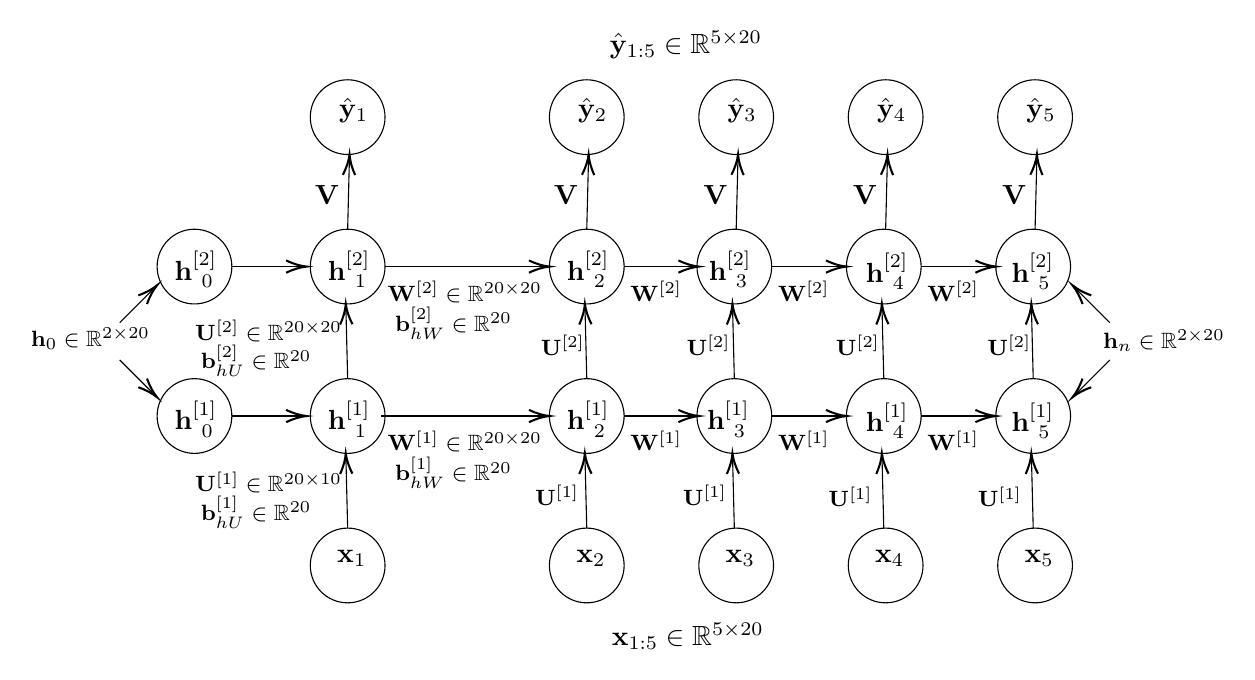
\begin{tikzpicture}[x=0.75pt,y=0.75pt,yscale=-0.9,xscale=0.9] 
        %Shape: Ellipse [id:dp4207915429094031] 
        \draw   (162,300) .. controls (162,288.95) and (170.95,280) .. (182,280) .. controls (193.05,280) and (202,288.95) .. (202,300) .. controls (202,311.05) and (193.05,320) .. (182,320) .. controls (170.95,320) and (162,311.05) .. (162,300) -- cycle ;
        %Straight Lines [id:da05829660867376418] 
        \draw [color={rgb, 255:red, 0; green, 0; blue, 0 }  ,draw opacity=1 ]   (182,280) -- (181.05,242) ;
        \draw [shift={(181,240)}, rotate = 88.57] [color={rgb, 255:red, 0; green, 0; blue, 0 }  ,draw opacity=1 ][line width=0.75]    (10.93,-3.29) .. controls (6.95,-1.4) and (3.31,-0.3) .. (0,0) .. controls (3.31,0.3) and (6.95,1.4) .. (10.93,3.29)   ;
        %Straight Lines [id:da5226654860183346] 
        \draw [color={rgb, 255:red, 0; green, 0; blue, 0 }  ,draw opacity=1 ]   (389,280) -- (388.05,242) ;
        \draw [shift={(388,240)}, rotate = 88.57] [color={rgb, 255:red, 0; green, 0; blue, 0 }  ,draw opacity=1 ][line width=0.75]    (10.93,-3.29) .. controls (6.95,-1.4) and (3.31,-0.3) .. (0,0) .. controls (3.31,0.3) and (6.95,1.4) .. (10.93,3.29)   ;
        %Straight Lines [id:da8260164672182386] 
        \draw [color={rgb, 255:red, 0; green, 0; blue, 0 }  ,draw opacity=1 ]   (469,280) -- (468.05,242) ;
        \draw [shift={(468,240)}, rotate = 88.57] [color={rgb, 255:red, 0; green, 0; blue, 0 }  ,draw opacity=1 ][line width=0.75]    (10.93,-3.29) .. controls (6.95,-1.4) and (3.31,-0.3) .. (0,0) .. controls (3.31,0.3) and (6.95,1.4) .. (10.93,3.29)   ;
        %Straight Lines [id:da9134708342055928] 
        \draw [color={rgb, 255:red, 0; green, 0; blue, 0 }  ,draw opacity=1 ]   (549,280) -- (548.05,242) ;
        \draw [shift={(548,240)}, rotate = 88.57] [color={rgb, 255:red, 0; green, 0; blue, 0 }  ,draw opacity=1 ][line width=0.75]    (10.93,-3.29) .. controls (6.95,-1.4) and (3.31,-0.3) .. (0,0) .. controls (3.31,0.3) and (6.95,1.4) .. (10.93,3.29)   ;
        %Shape: Ellipse [id:dp025885252304979955] 
        \draw   (369,220) .. controls (369,208.95) and (377.95,200) .. (389,200) .. controls (400.05,200) and (409,208.95) .. (409,220) .. controls (409,231.05) and (400.05,240) .. (389,240) .. controls (377.95,240) and (369,231.05) .. (369,220) -- cycle ;
        %Shape: Ellipse [id:dp7180898602484265] 
        \draw   (529,220) .. controls (529,208.95) and (537.95,200) .. (549,200) .. controls (560.05,200) and (569,208.95) .. (569,220) .. controls (569,231.05) and (560.05,240) .. (549,240) .. controls (537.95,240) and (529,231.05) .. (529,220) -- cycle ;
        %Shape: Ellipse [id:dp888584652011154] 
        \draw   (449,220) .. controls (449,208.95) and (457.95,200) .. (469,200) .. controls (480.05,200) and (489,208.95) .. (489,220) .. controls (489,231.05) and (480.05,240) .. (469,240) .. controls (457.95,240) and (449,231.05) .. (449,220) -- cycle ;
        %Shape: Ellipse [id:dp770959326042951] 
        \draw   (162,220) .. controls (162,208.95) and (170.95,200) .. (182,200) .. controls (193.05,200) and (202,208.95) .. (202,220) .. controls (202,231.05) and (193.05,240) .. (182,240) .. controls (170.95,240) and (162,231.05) .. (162,220) -- cycle ;
        %Straight Lines [id:da02863489015429077] 
        \draw [color={rgb, 255:red, 0; green, 0; blue, 0 }  ,draw opacity=1 ]   (409,220) -- (447,220) ;
        \draw [shift={(449,220)}, rotate = 180] [color={rgb, 255:red, 0; green, 0; blue, 0 }  ,draw opacity=1 ][line width=0.75]    (10.93,-3.29) .. controls (6.95,-1.4) and (3.31,-0.3) .. (0,0) .. controls (3.31,0.3) and (6.95,1.4) .. (10.93,3.29)   ;
        %Straight Lines [id:da28454183440455316] 
        \draw [color={rgb, 255:red, 0; green, 0; blue, 0 }  ,draw opacity=1 ]   (489,220) -- (527,220) ;
        \draw [shift={(529,220)}, rotate = 180] [color={rgb, 255:red, 0; green, 0; blue, 0 }  ,draw opacity=1 ][line width=0.75]    (10.93,-3.29) .. controls (6.95,-1.4) and (3.31,-0.3) .. (0,0) .. controls (3.31,0.3) and (6.95,1.4) .. (10.93,3.29)   ;
        %Straight Lines [id:da4244979895569312] 
        \draw [color={rgb, 255:red, 0; green, 0; blue, 0 }  ,draw opacity=1 ]   (182,200) -- (181.05,162) ;
        \draw [shift={(181,160)}, rotate = 88.57] [color={rgb, 255:red, 0; green, 0; blue, 0 }  ,draw opacity=1 ][line width=0.75]    (10.93,-3.29) .. controls (6.95,-1.4) and (3.31,-0.3) .. (0,0) .. controls (3.31,0.3) and (6.95,1.4) .. (10.93,3.29)   ;
        %Straight Lines [id:da41291607651105977] 
        \draw [color={rgb, 255:red, 0; green, 0; blue, 0 }  ,draw opacity=1 ]   (389,200) -- (388.05,162) ;
        \draw [shift={(388,160)}, rotate = 88.57] [color={rgb, 255:red, 0; green, 0; blue, 0 }  ,draw opacity=1 ][line width=0.75]    (10.93,-3.29) .. controls (6.95,-1.4) and (3.31,-0.3) .. (0,0) .. controls (3.31,0.3) and (6.95,1.4) .. (10.93,3.29)   ;
        %Straight Lines [id:da5340101186518054] 
        \draw [color={rgb, 255:red, 0; green, 0; blue, 0 }  ,draw opacity=1 ]   (469,200) -- (468.05,162) ;
        \draw [shift={(468,160)}, rotate = 88.57] [color={rgb, 255:red, 0; green, 0; blue, 0 }  ,draw opacity=1 ][line width=0.75]    (10.93,-3.29) .. controls (6.95,-1.4) and (3.31,-0.3) .. (0,0) .. controls (3.31,0.3) and (6.95,1.4) .. (10.93,3.29)   ;
        %Straight Lines [id:da7929637636987212] 
        \draw [color={rgb, 255:red, 0; green, 0; blue, 0 }  ,draw opacity=1 ]   (549,200) -- (548.05,162) ;
        \draw [shift={(548,160)}, rotate = 88.57] [color={rgb, 255:red, 0; green, 0; blue, 0 }  ,draw opacity=1 ][line width=0.75]    (10.93,-3.29) .. controls (6.95,-1.4) and (3.31,-0.3) .. (0,0) .. controls (3.31,0.3) and (6.95,1.4) .. (10.93,3.29)   ;
        %Shape: Ellipse [id:dp8354295005953776] 
        \draw   (369,140) .. controls (369,128.95) and (377.95,120) .. (389,120) .. controls (400.05,120) and (409,128.95) .. (409,140) .. controls (409,151.05) and (400.05,160) .. (389,160) .. controls (377.95,160) and (369,151.05) .. (369,140) -- cycle ;
        %Shape: Ellipse [id:dp8165367609646754] 
        \draw   (529,140) .. controls (529,128.95) and (537.95,120) .. (549,120) .. controls (560.05,120) and (569,128.95) .. (569,140) .. controls (569,151.05) and (560.05,160) .. (549,160) .. controls (537.95,160) and (529,151.05) .. (529,140) -- cycle ;
        %Shape: Ellipse [id:dp20706274445577244] 
        \draw   (449,140) .. controls (449,128.95) and (457.95,120) .. (469,120) .. controls (480.05,120) and (489,128.95) .. (489,140) .. controls (489,151.05) and (480.05,160) .. (469,160) .. controls (457.95,160) and (449,151.05) .. (449,140) -- cycle ;
        %Shape: Ellipse [id:dp028074370298882823] 
        \draw   (162,140) .. controls (162,128.95) and (170.95,120) .. (182,120) .. controls (193.05,120) and (202,128.95) .. (202,140) .. controls (202,151.05) and (193.05,160) .. (182,160) .. controls (170.95,160) and (162,151.05) .. (162,140) -- cycle ;
        %Straight Lines [id:da40086305523058074] 
        \draw [color={rgb, 255:red, 0; green, 0; blue, 0 }  ,draw opacity=1 ]   (409,140) -- (447,140) ;
        \draw [shift={(449,140)}, rotate = 180] [color={rgb, 255:red, 0; green, 0; blue, 0 }  ,draw opacity=1 ][line width=0.75]    (10.93,-3.29) .. controls (6.95,-1.4) and (3.31,-0.3) .. (0,0) .. controls (3.31,0.3) and (6.95,1.4) .. (10.93,3.29)   ;
        %Straight Lines [id:da3677135880821485] 
        \draw [color={rgb, 255:red, 0; green, 0; blue, 0 }  ,draw opacity=1 ]   (489,140) -- (527,140) ;
        \draw [shift={(529,140)}, rotate = 180] [color={rgb, 255:red, 0; green, 0; blue, 0 }  ,draw opacity=1 ][line width=0.75]    (10.93,-3.29) .. controls (6.95,-1.4) and (3.31,-0.3) .. (0,0) .. controls (3.31,0.3) and (6.95,1.4) .. (10.93,3.29)   ;
        %Shape: Ellipse [id:dp2624210064078889] 
        \draw   (80,140) .. controls (80,128.95) and (88.95,120) .. (100,120) .. controls (111.05,120) and (120,128.95) .. (120,140) .. controls (120,151.05) and (111.05,160) .. (100,160) .. controls (88.95,160) and (80,151.05) .. (80,140) -- cycle ;
        %Straight Lines [id:da4871181057362928] 
        \draw [color={rgb, 255:red, 0; green, 0; blue, 0 }  ,draw opacity=1 ]   (120,140) -- (158,140) ;
        \draw [shift={(160,140)}, rotate = 180] [color={rgb, 255:red, 0; green, 0; blue, 0 }  ,draw opacity=1 ][line width=0.75]    (10.93,-3.29) .. controls (6.95,-1.4) and (3.31,-0.3) .. (0,0) .. controls (3.31,0.3) and (6.95,1.4) .. (10.93,3.29)   ;
        %Shape: Ellipse [id:dp5872757033401736] 
        \draw   (80,220) .. controls (80,208.95) and (88.95,200) .. (100,200) .. controls (111.05,200) and (120,208.95) .. (120,220) .. controls (120,231.05) and (111.05,240) .. (100,240) .. controls (88.95,240) and (80,231.05) .. (80,220) -- cycle ;
        %Straight Lines [id:da2475482028591074] 
        \draw [color={rgb, 255:red, 0; green, 0; blue, 0 }  ,draw opacity=1 ]   (120,220) -- (158,220) ;
        \draw [shift={(160,220)}, rotate = 180] [color={rgb, 255:red, 0; green, 0; blue, 0 }  ,draw opacity=1 ][line width=0.75]    (10.93,-3.29) .. controls (6.95,-1.4) and (3.31,-0.3) .. (0,0) .. controls (3.31,0.3) and (6.95,1.4) .. (10.93,3.29)   ;
        %Straight Lines [id:da9282104785993115] 
        \draw [color={rgb, 255:red, 0; green, 0; blue, 0 }  ,draw opacity=1 ]   (200,220) -- (288,220) ;
        \draw [shift={(290,220)}, rotate = 180] [color={rgb, 255:red, 0; green, 0; blue, 0 }  ,draw opacity=1 ][line width=0.75]    (10.93,-3.29) .. controls (6.95,-1.4) and (3.31,-0.3) .. (0,0) .. controls (3.31,0.3) and (6.95,1.4) .. (10.93,3.29)   ;
        %Straight Lines [id:da17558336312768597] 
        \draw [color={rgb, 255:red, 0; green, 0; blue, 0 }  ,draw opacity=1 ]   (202,140) -- (272,140) -- (288,140) ;
        \draw [shift={(290,140)}, rotate = 180] [color={rgb, 255:red, 0; green, 0; blue, 0 }  ,draw opacity=1 ][line width=0.75]    (10.93,-3.29) .. controls (6.95,-1.4) and (3.31,-0.3) .. (0,0) .. controls (3.31,0.3) and (6.95,1.4) .. (10.93,3.29)   ;
        %Shape: Ellipse [id:dp6255666224284429] 
        \draw   (290,300) .. controls (290,288.95) and (298.95,280) .. (310,280) .. controls (321.05,280) and (330,288.95) .. (330,300) .. controls (330,311.05) and (321.05,320) .. (310,320) .. controls (298.95,320) and (290,311.05) .. (290,300) -- cycle ;
        %Straight Lines [id:da10727200987868368] 
        \draw [color={rgb, 255:red, 0; green, 0; blue, 0 }  ,draw opacity=1 ]   (310,280) -- (309.05,242) ;
        \draw [shift={(309,240)}, rotate = 88.57] [color={rgb, 255:red, 0; green, 0; blue, 0 }  ,draw opacity=1 ][line width=0.75]    (10.93,-3.29) .. controls (6.95,-1.4) and (3.31,-0.3) .. (0,0) .. controls (3.31,0.3) and (6.95,1.4) .. (10.93,3.29)   ;
        %Shape: Ellipse [id:dp8818598215343834] 
        \draw   (290,220) .. controls (290,208.95) and (298.95,200) .. (310,200) .. controls (321.05,200) and (330,208.95) .. (330,220) .. controls (330,231.05) and (321.05,240) .. (310,240) .. controls (298.95,240) and (290,231.05) .. (290,220) -- cycle ;
        %Straight Lines [id:da35172171925239026] 
        \draw [color={rgb, 255:red, 0; green, 0; blue, 0 }  ,draw opacity=1 ]   (310,200) -- (309.05,162) ;
        \draw [shift={(309,160)}, rotate = 88.57] [color={rgb, 255:red, 0; green, 0; blue, 0 }  ,draw opacity=1 ][line width=0.75]    (10.93,-3.29) .. controls (6.95,-1.4) and (3.31,-0.3) .. (0,0) .. controls (3.31,0.3) and (6.95,1.4) .. (10.93,3.29)   ;
        %Shape: Ellipse [id:dp27873635132142716] 
        \draw   (290,140) .. controls (290,128.95) and (298.95,120) .. (310,120) .. controls (321.05,120) and (330,128.95) .. (330,140) .. controls (330,151.05) and (321.05,160) .. (310,160) .. controls (298.95,160) and (290,151.05) .. (290,140) -- cycle ;
        %Straight Lines [id:da38304549426248236] 
        \draw [color={rgb, 255:red, 0; green, 0; blue, 0 }  ,draw opacity=1 ]   (330,220) -- (368,220) ;
        \draw [shift={(370,220)}, rotate = 180] [color={rgb, 255:red, 0; green, 0; blue, 0 }  ,draw opacity=1 ][line width=0.75]    (10.93,-3.29) .. controls (6.95,-1.4) and (3.31,-0.3) .. (0,0) .. controls (3.31,0.3) and (6.95,1.4) .. (10.93,3.29)   ;
        %Straight Lines [id:da57208010142451] 
        \draw [color={rgb, 255:red, 0; green, 0; blue, 0 }  ,draw opacity=1 ]   (330,140) -- (368,140) ;
        \draw [shift={(370,140)}, rotate = 180] [color={rgb, 255:red, 0; green, 0; blue, 0 }  ,draw opacity=1 ][line width=0.75]    (10.93,-3.29) .. controls (6.95,-1.4) and (3.31,-0.3) .. (0,0) .. controls (3.31,0.3) and (6.95,1.4) .. (10.93,3.29)   ;
        %Straight Lines [id:da5663542407709887] 
        \draw [color={rgb, 255:red, 0; green, 0; blue, 0 }  ,draw opacity=1 ]   (390,120) -- (390.95,82) ;
        \draw [shift={(391,80)}, rotate = 91.43] [color={rgb, 255:red, 0; green, 0; blue, 0 }  ,draw opacity=1 ][line width=0.75]    (10.93,-3.29) .. controls (6.95,-1.4) and (3.31,-0.3) .. (0,0) .. controls (3.31,0.3) and (6.95,1.4) .. (10.93,3.29)   ;
        %Straight Lines [id:da32507454347747866] 
        \draw [color={rgb, 255:red, 0; green, 0; blue, 0 }  ,draw opacity=1 ]   (470,120) -- (470.95,82) ;
        \draw [shift={(471,80)}, rotate = 91.43] [color={rgb, 255:red, 0; green, 0; blue, 0 }  ,draw opacity=1 ][line width=0.75]    (10.93,-3.29) .. controls (6.95,-1.4) and (3.31,-0.3) .. (0,0) .. controls (3.31,0.3) and (6.95,1.4) .. (10.93,3.29)   ;
        %Straight Lines [id:da9828329348785247] 
        \draw [color={rgb, 255:red, 0; green, 0; blue, 0 }  ,draw opacity=1 ]   (550,120) -- (550.95,82) ;
        \draw [shift={(551,80)}, rotate = 91.43] [color={rgb, 255:red, 0; green, 0; blue, 0 }  ,draw opacity=1 ][line width=0.75]    (10.93,-3.29) .. controls (6.95,-1.4) and (3.31,-0.3) .. (0,0) .. controls (3.31,0.3) and (6.95,1.4) .. (10.93,3.29)   ;
        %Straight Lines [id:da21940187807374456] 
        \draw [color={rgb, 255:red, 0; green, 0; blue, 0 }  ,draw opacity=1 ]   (182,120) -- (182.95,82) ;
        \draw [shift={(183,80)}, rotate = 91.43] [color={rgb, 255:red, 0; green, 0; blue, 0 }  ,draw opacity=1 ][line width=0.75]    (10.93,-3.29) .. controls (6.95,-1.4) and (3.31,-0.3) .. (0,0) .. controls (3.31,0.3) and (6.95,1.4) .. (10.93,3.29)   ;
        %Straight Lines [id:da9515990853220169] 
        \draw [color={rgb, 255:red, 0; green, 0; blue, 0 }  ,draw opacity=1 ]   (310,120) -- (310.95,82) ;
        \draw [shift={(311,80)}, rotate = 91.43] [color={rgb, 255:red, 0; green, 0; blue, 0 }  ,draw opacity=1 ][line width=0.75]    (10.93,-3.29) .. controls (6.95,-1.4) and (3.31,-0.3) .. (0,0) .. controls (3.31,0.3) and (6.95,1.4) .. (10.93,3.29)   ;
        %Shape: Ellipse [id:dp7031207995591184] 
        \draw   (162,60) .. controls (162,48.95) and (170.95,40) .. (182,40) .. controls (193.05,40) and (202,48.95) .. (202,60) .. controls (202,71.05) and (193.05,80) .. (182,80) .. controls (170.95,80) and (162,71.05) .. (162,60) -- cycle ;
        %Shape: Ellipse [id:dp4918664633020191] 
        \draw   (290,60) .. controls (290,48.95) and (298.95,40) .. (310,40) .. controls (321.05,40) and (330,48.95) .. (330,60) .. controls (330,71.05) and (321.05,80) .. (310,80) .. controls (298.95,80) and (290,71.05) .. (290,60) -- cycle ;
        %Shape: Ellipse [id:dp678788283809618] 
        \draw   (370,60) .. controls (370,48.95) and (378.95,40) .. (390,40) .. controls (401.05,40) and (410,48.95) .. (410,60) .. controls (410,71.05) and (401.05,80) .. (390,80) .. controls (378.95,80) and (370,71.05) .. (370,60) -- cycle ;
        %Shape: Ellipse [id:dp40410246110864323] 
        \draw   (450,60) .. controls (450,48.95) and (458.95,40) .. (470,40) .. controls (481.05,40) and (490,48.95) .. (490,60) .. controls (490,71.05) and (481.05,80) .. (470,80) .. controls (458.95,80) and (450,71.05) .. (450,60) -- cycle ;
        %Shape: Ellipse [id:dp357818602045721] 
        \draw   (530,60) .. controls (530,48.95) and (538.95,40) .. (550,40) .. controls (561.05,40) and (570,48.95) .. (570,60) .. controls (570,71.05) and (561.05,80) .. (550,80) .. controls (538.95,80) and (530,71.05) .. (530,60) -- cycle ;
        %Shape: Ellipse [id:dp861370706015621] 
        \draw   (370,300) .. controls (370,288.95) and (378.95,280) .. (390,280) .. controls (401.05,280) and (410,288.95) .. (410,300) .. controls (410,311.05) and (401.05,320) .. (390,320) .. controls (378.95,320) and (370,311.05) .. (370,300) -- cycle ;
        %Shape: Ellipse [id:dp10149404856059419] 
        \draw   (450,300) .. controls (450,288.95) and (458.95,280) .. (470,280) .. controls (481.05,280) and (490,288.95) .. (490,300) .. controls (490,311.05) and (481.05,320) .. (470,320) .. controls (458.95,320) and (450,311.05) .. (450,300) -- cycle ;
        %Shape: Ellipse [id:dp5054375673565727] 
        \draw   (530,300) .. controls (530,288.95) and (538.95,280) .. (550,280) .. controls (561.05,280) and (570,288.95) .. (570,300) .. controls (570,311.05) and (561.05,320) .. (550,320) .. controls (538.95,320) and (530,311.05) .. (530,300) -- cycle ;
        %Straight Lines [id:da48642808985309793] 
        \draw    (60,170) -- (78.59,151.41) ;
        \draw [shift={(80,150)}, rotate = 135] [color={rgb, 255:red, 0; green, 0; blue, 0 }  ][line width=0.75]    (10.93,-3.29) .. controls (6.95,-1.4) and (3.31,-0.3) .. (0,0) .. controls (3.31,0.3) and (6.95,1.4) .. (10.93,3.29)   ;
        %Straight Lines [id:da622558990053925] 
        \draw    (60,190) -- (78.59,208.59) ;
        \draw [shift={(80,210)}, rotate = 225] [color={rgb, 255:red, 0; green, 0; blue, 0 }  ][line width=0.75]    (10.93,-3.29) .. controls (6.95,-1.4) and (3.31,-0.3) .. (0,0) .. controls (3.31,0.3) and (6.95,1.4) .. (10.93,3.29)   ;
        %Straight Lines [id:da4475932343558764] 
        \draw    (590,170) -- (571.41,151.41) ;
        \draw [shift={(570,150)}, rotate = 45] [color={rgb, 255:red, 0; green, 0; blue, 0 }  ][line width=0.75]    (10.93,-3.29) .. controls (6.95,-1.4) and (3.31,-0.3) .. (0,0) .. controls (3.31,0.3) and (6.95,1.4) .. (10.93,3.29)   ;
        %Straight Lines [id:da7531844960895331] 
        \draw    (590,190) -- (571.41,208.59) ;
        \draw [shift={(570,210)}, rotate = 315] [color={rgb, 255:red, 0; green, 0; blue, 0 }  ][line width=0.75]    (10.93,-3.29) .. controls (6.95,-1.4) and (3.31,-0.3) .. (0,0) .. controls (3.31,0.3) and (6.95,1.4) .. (10.93,3.29)   ;

        % Text Node
        \draw (175,290.4) node [anchor=north west][inner sep=0.75pt]  [font=\normalsize]  {$\mathbf{x}_{1}$};
        % Text Node
        \draw (360,255.4) node [anchor=north west][inner sep=0.75pt]  [font=\footnotesize,color={rgb, 255:red, 0; green, 0; blue, 0 }  ,opacity=1 ]  {$\mathbf{U}^{[ 1]}$};
        % Text Node
        \draw (438,256.4) node [anchor=north west][inner sep=0.75pt]  [font=\footnotesize,color={rgb, 255:red, 0; green, 0; blue, 0 }  ,opacity=1 ]  {$\mathbf{U}^{[ 1]}$};
        % Text Node
        \draw (518,256.4) node [anchor=north west][inner sep=0.75pt]  [font=\footnotesize,color={rgb, 255:red, 0; green, 0; blue, 0 }  ,opacity=1 ]  {$\mathbf{U}^{[ 1]}$};
        % Text Node
        \draw (170,210.4) node [anchor=north west][inner sep=0.75pt]  [font=\normalsize]  {$\mathbf{h}_{\ 1}^{[ 1]}$};
        % Text Node
        \draw (373,210.4) node [anchor=north west][inner sep=0.75pt]  [font=\normalsize]  {$\mathbf{h}_{\ 3}^{[ 1]}$};
        % Text Node
        \draw (458,211.4) node [anchor=north west][inner sep=0.75pt]  [font=\normalsize]  {$\mathbf{h}_{\ 4}^{[ 1]}$};
        % Text Node
        \draw (536,211.4) node [anchor=north west][inner sep=0.75pt]  [font=\normalsize]  {$\mathbf{h}_{\ 5}^{[ 1]}$};
        % Text Node
        \draw (411,226.4) node [anchor=north west][inner sep=0.75pt]  [font=\footnotesize,color={rgb, 255:red, 0; green, 0; blue, 0 }  ,opacity=1 ]  {$\mathbf{W}^{[ 1]}$};
        % Text Node
        \draw (491,226.4) node [anchor=north west][inner sep=0.75pt]  [font=\footnotesize,color={rgb, 255:red, 0; green, 0; blue, 0 }  ,opacity=1 ]  {$\mathbf{W}^{[ 1]}$};
        % Text Node
        \draw (99,167.4) node [anchor=north west][inner sep=0.75pt]  [font=\footnotesize,color={rgb, 255:red, 0; green, 0; blue, 0 }  ,opacity=1 ]  {$\mathbf{U}^{[ 2]} \in \mathbb{R}^{20\times 20}$};
        % Text Node
        \draw (362,175.4) node [anchor=north west][inner sep=0.75pt]  [font=\footnotesize,color={rgb, 255:red, 0; green, 0; blue, 0 }  ,opacity=1 ]  {$\mathbf{U}^{[ 2]}$};
        % Text Node
        \draw (442,175.4) node [anchor=north west][inner sep=0.75pt]  [font=\footnotesize,color={rgb, 255:red, 0; green, 0; blue, 0 }  ,opacity=1 ]  {$\mathbf{U}^{[ 2]}$};
        % Text Node
        \draw (523,175.4) node [anchor=north west][inner sep=0.75pt]  [font=\footnotesize,color={rgb, 255:red, 0; green, 0; blue, 0 }  ,opacity=1 ]  {$\mathbf{U}^{[ 2]}$};
        % Text Node
        \draw (170,130.4) node [anchor=north west][inner sep=0.75pt]  [font=\normalsize]  {$\mathbf{h}_{\ 1}^{[ 2]}$};
        % Text Node
        \draw (374,130.4) node [anchor=north west][inner sep=0.75pt]  [font=\normalsize]  {$\mathbf{h}_{\ 3}^{[ 2]}$};
        % Text Node
        \draw (458,131.4) node [anchor=north west][inner sep=0.75pt]  [font=\normalsize]  {$\mathbf{h}_{\ 4}^{[ 2]}$};
        % Text Node
        \draw (536,131.4) node [anchor=north west][inner sep=0.75pt]  [font=\normalsize]  {$\mathbf{h}_{\ 5}^{[ 2]}$};
        % Text Node
        \draw (411,146.4) node [anchor=north west][inner sep=0.75pt]  [font=\footnotesize,color={rgb, 255:red, 0; green, 0; blue, 0 }  ,opacity=1 ]  {$\mathbf{W}^{[ 2]}$};
        % Text Node
        \draw (491,146.4) node [anchor=north west][inner sep=0.75pt]  [font=\footnotesize,color={rgb, 255:red, 0; green, 0; blue, 0 }  ,opacity=1 ]  {$\mathbf{W}^{[ 2]}$};
        % Text Node
        \draw (88,130.4) node [anchor=north west][inner sep=0.75pt]  [font=\normalsize]  {$\mathbf{h}_{\ 0}^{[ 2]}$};
        % Text Node
        \draw (88,210.4) node [anchor=north west][inner sep=0.75pt]  [font=\normalsize]  {$\mathbf{h}_{\ 0}^{[ 1]}$};
        % Text Node
        \draw (202,146.4) node [anchor=north west][inner sep=0.75pt]  [font=\footnotesize,color={rgb, 255:red, 0; green, 0; blue, 0 }  ,opacity=1 ]  {$\mathbf{W}^{[ 2]} \in \mathbb{R}^{20\times 20}$};
        % Text Node
        \draw (303,290.4) node [anchor=north west][inner sep=0.75pt]  [font=\normalsize]  {$\mathbf{x}_{2}$};
        % Text Node
        \draw (281,255.4) node [anchor=north west][inner sep=0.75pt]  [font=\footnotesize,color={rgb, 255:red, 0; green, 0; blue, 0 }  ,opacity=1 ]  {$\mathbf{U}^{[ 1]}$};
        % Text Node
        \draw (298,210.4) node [anchor=north west][inner sep=0.75pt]  [font=\normalsize]  {$\mathbf{h}_{\ 2}^{[ 1]}$};
        % Text Node
        \draw (284,175.4) node [anchor=north west][inner sep=0.75pt]  [font=\footnotesize,color={rgb, 255:red, 0; green, 0; blue, 0 }  ,opacity=1 ]  {$\mathbf{U}^{[ 2]}$};
        % Text Node
        \draw (298,130.4) node [anchor=north west][inner sep=0.75pt]  [font=\normalsize]  {$\mathbf{h}_{\ 2}^{[ 2]}$};
        % Text Node
        \draw (332,226.4) node [anchor=north west][inner sep=0.75pt]  [font=\footnotesize,color={rgb, 255:red, 0; green, 0; blue, 0 }  ,opacity=1 ]  {$\mathbf{W}^{[ 1]}$};
        % Text Node
        \draw (332,146.4) node [anchor=north west][inner sep=0.75pt]  [font=\footnotesize,color={rgb, 255:red, 0; green, 0; blue, 0 }  ,opacity=1 ]  {$\mathbf{W}^{[ 2]}$};
        % Text Node
        \draw (371,95.4) node [anchor=north west][inner sep=0.75pt]  [font=\normalsize,color={rgb, 255:red, 0; green, 0; blue, 0 }  ,opacity=1 ]  {$\mathbf{V}$};
        % Text Node
        \draw (451,95.4) node [anchor=north west][inner sep=0.75pt]  [font=\normalsize,color={rgb, 255:red, 0; green, 0; blue, 0 }  ,opacity=1 ]  {$\mathbf{V}$};
        % Text Node
        \draw (531,95.4) node [anchor=north west][inner sep=0.75pt]  [font=\normalsize,color={rgb, 255:red, 0; green, 0; blue, 0 }  ,opacity=1 ]  {$\mathbf{V}$};
        % Text Node
        \draw (163,95.4) node [anchor=north west][inner sep=0.75pt]  [font=\normalsize,color={rgb, 255:red, 0; green, 0; blue, 0 }  ,opacity=1 ]  {$\mathbf{V}$};
        % Text Node
        \draw (291,95.4) node [anchor=north west][inner sep=0.75pt]  [font=\normalsize,color={rgb, 255:red, 0; green, 0; blue, 0 }  ,opacity=1 ]  {$\mathbf{V}$};
        % Text Node
        \draw (176,48.4) node [anchor=north west][inner sep=0.75pt]  [font=\normalsize]  {$\hat{\mathbf{y}}_{1}$};
        % Text Node
        \draw (304,48.4) node [anchor=north west][inner sep=0.75pt]  [font=\normalsize]  {$\hat{\mathbf{y}}_{2}$};
        % Text Node
        \draw (384,48.4) node [anchor=north west][inner sep=0.75pt]  [font=\normalsize]  {$\hat{\mathbf{y}}_{3}$};
        % Text Node
        \draw (464,48.4) node [anchor=north west][inner sep=0.75pt]  [font=\normalsize]  {$\hat{\mathbf{y}}_{4}$};
        % Text Node
        \draw (544,48.4) node [anchor=north west][inner sep=0.75pt]  [font=\normalsize]  {$\hat{\mathbf{y}}_{5}$};
        % Text Node
        \draw (383,290.4) node [anchor=north west][inner sep=0.75pt]  [font=\normalsize]  {$\mathbf{x}_{3}$};
        % Text Node
        \draw (463,290.4) node [anchor=north west][inner sep=0.75pt]  [font=\normalsize]  {$\mathbf{x}_{4}$};
        % Text Node
        \draw (543,290.4) node [anchor=north west][inner sep=0.75pt]  [font=\normalsize]  {$\mathbf{x}_{5}$};
        % Text Node
        \draw (202,226.4) node [anchor=north west][inner sep=0.75pt]  [font=\footnotesize,color={rgb, 255:red, 0; green, 0; blue, 0 }  ,opacity=1 ]  {$\mathbf{W}^{[ 1]} \in \mathbb{R}^{20\times 20}$};
        % Text Node
        \draw (99,248.4) node [anchor=north west][inner sep=0.75pt]  [font=\footnotesize,color={rgb, 255:red, 0; green, 0; blue, 0 }  ,opacity=1 ]  {$\mathbf{U}^{[ 1]} \in \mathbb{R}^{20\times 10}$};
        % Text Node
        \draw (102,261.4) node [anchor=north west][inner sep=0.75pt]  [font=\footnotesize,color={rgb, 255:red, 0; green, 0; blue, 0 }  ,opacity=1 ]  {$\mathbf{b}_{hU}^{[ 1]} \in \mathbb{R}^{20}$};
        % Text Node
        \draw (102,180.4) node [anchor=north west][inner sep=0.75pt]  [font=\footnotesize,color={rgb, 255:red, 0; green, 0; blue, 0 }  ,opacity=1 ]  {$\mathbf{b}_{hU}^{[ 2]} \in \mathbb{R}^{20}$};
        % Text Node
        \draw (206,160.4) node [anchor=north west][inner sep=0.75pt]  [font=\footnotesize,color={rgb, 255:red, 0; green, 0; blue, 0 }  ,opacity=1 ]  {$\mathbf{b}_{hW}^{[ 2]} \in \mathbb{R}^{20}$};
        % Text Node
        \draw (206,240.4) node [anchor=north west][inner sep=0.75pt]  [font=\footnotesize,color={rgb, 255:red, 0; green, 0; blue, 0 }  ,opacity=1 ]  {$\mathbf{b}_{hW}^{[ 1]} \in \mathbb{R}^{20}$};
        % Text Node
        \draw (11,171.4) node [anchor=north west][inner sep=0.75pt]  [font=\footnotesize]  {$\mathbf{h}_{0} \in \mathbb{R}^{2\times 20}$};
        % Text Node
        \draw (585,172.4) node [anchor=north west][inner sep=0.75pt]  [font=\footnotesize]  {$\mathbf{h}_{n} \in \mathbb{R}^{2\times 20}$};
        % Text Node
        \draw (322,329.4) node [anchor=north west][inner sep=0.75pt]  [font=\normalsize]  {$\mathbf{x}_{1:5} \in \mathbb{R}^{5\times 20}$};
        % Text Node
        \draw (321,12.4) node [anchor=north west][inner sep=0.75pt]  [font=\normalsize]  {$\hat{\mathbf{y}}_{1:5} \in \mathbb{R}^{5\times 20}$};
      \end{tikzpicture}
      \caption{}
      \label{fig:rnn_pytorch_rnn}
    \end{figure}

    As we expect, there are 8 vectors/matrices we must optimize: $\mathbf{W}^{[1]}, \mathbf{W}^{[2]}, \mathbf{U}^{[1]}, \mathbf{U}^{[2]}, \mathbf{b}^{[1]}_{hU}, \mathbf{b}^{[1]}_{hW}, \mathbf{b}^{[2]}_{hW}, \mathbf{b}^{[2]}_{hU}$. 

\subsection{Long Short Term Memory (LSTMs)}

  In theory, RNNs are very beautiful and can be applied in all cases, but in practice they do not perform very well, mainly due to the vanishing/exploding gradient problem. 
  \begin{enumerate}
    \item An exploding gradient is easy to fix, since we can just use the max-norm regularization, i.e. \textbf{gradient clipping}, to just set a max vamlue for the gradients if they grow too large. 
    \item The \textbf{truncated backpropagation through time} (TBPTT) simply limits the number of times steps the signal can backpropagate after each forward pass, e.g. even if the sequence has 100 time steps, we may only backpropagate through 20 or so. 
    \item The \textbf{LSTM} model uses a memory cell for modeling long-range dependencies and avoids the vanishing gradient problems. 
  \end{enumerate}

  Historically LSTMs were used in achieving state-of-the-art results in 2013 through 2015, in tasks such as handwriting recognition, speech recognition, machine translation, parsing, and image captioning, as well as language models. They became to dominant approach for most NLP tasks, but in 2021, they have been overshadowed by transformer models, which we will talk about next. 

  LSTMs have a much more complicated unit to work with, so let's go through it slowly. Note that so far, a one-layer RNN consisted of recursive mappings of the form 
  \begin{equation}
    (\mathbf{x}_t, \mathbf{h}_{t-1}) \mapsto ( \mathbf{h}_t, \hat{\mathbf{y}}_t)
  \end{equation}
  We can interpret the vector $\mathbf{h}_{t-1}$ as the \textbf{short term memory}, or \textbf{hidden state}, that contains information used to predict the next output value. However, this can be corrupted (e.g. forgetting information from many steps ago), so we add an additional \textbf{long term memory}, or \textbf{cell state}, vector $\mathbf{c}_t$ that should be preserved. Therefore, we have two arrows coming out of each hidden layer, as shown below in the one-layer LSTM. 

  \begin{figure}[H]
    \centering 
    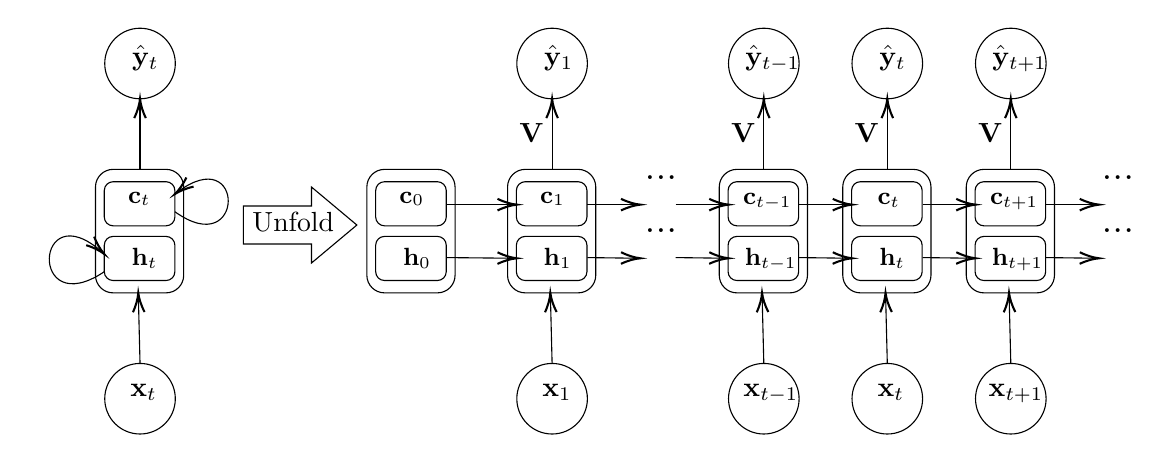
\begin{tikzpicture}[x=0.75pt,y=0.75pt,yscale=-0.85,xscale=0.85]
      %Rounded Rect [id:dp9162379150448552] 
      \draw   (36.18,110) .. controls (36.18,104.48) and (40.66,100) .. (46.18,100) -- (76.18,100) .. controls (81.71,100) and (86.18,104.48) .. (86.18,110) -- (86.18,160) .. controls (86.18,165.52) and (81.71,170) .. (76.18,170) -- (46.18,170) .. controls (40.66,170) and (36.18,165.52) .. (36.18,160) -- cycle ;
      %Rounded Rect [id:dp44390871530521614] 
      \draw   (41.18,112) .. controls (41.18,109.24) and (43.42,107) .. (46.18,107) -- (76.18,107) .. controls (78.95,107) and (81.18,109.24) .. (81.18,112) -- (81.18,127) .. controls (81.18,129.76) and (78.95,132) .. (76.18,132) -- (46.18,132) .. controls (43.42,132) and (41.18,129.76) .. (41.18,127) -- cycle ;
      %Rounded Rect [id:dp023212849697244353] 
      \draw   (41.18,143) .. controls (41.18,140.24) and (43.42,138) .. (46.18,138) -- (76.18,138) .. controls (78.95,138) and (81.18,140.24) .. (81.18,143) -- (81.18,158) .. controls (81.18,160.76) and (78.95,163) .. (76.18,163) -- (46.18,163) .. controls (43.42,163) and (41.18,160.76) .. (41.18,158) -- cycle ;
      %Curve Lines [id:da46664761054448833] 
      \draw [color={rgb, 255:red, 0; green, 0; blue, 0 }  ,draw opacity=1 ]   (81.18,124) .. controls (121.11,152.71) and (121.51,83.41) .. (82.38,113.07) ;
      \draw [shift={(81.18,114)}, rotate = 321.57] [color={rgb, 255:red, 0; green, 0; blue, 0 }  ,draw opacity=1 ][line width=0.75]    (10.93,-3.29) .. controls (6.95,-1.4) and (3.31,-0.3) .. (0,0) .. controls (3.31,0.3) and (6.95,1.4) .. (10.93,3.29)   ;
      %Curve Lines [id:da10224295018656915] 
      \draw [color={rgb, 255:red, 0; green, 0; blue, 0 }  ,draw opacity=1 ]   (41.18,158) .. controls (-1.94,186.93) and (1.55,112.73) .. (40.01,146.93) ;
      \draw [shift={(41.18,148)}, rotate = 222.92] [color={rgb, 255:red, 0; green, 0; blue, 0 }  ,draw opacity=1 ][line width=0.75]    (10.93,-3.29) .. controls (6.95,-1.4) and (3.31,-0.3) .. (0,0) .. controls (3.31,0.3) and (6.95,1.4) .. (10.93,3.29)   ;
      %Shape: Ellipse [id:dp6111375564351242] 
      \draw   (41.43,40) .. controls (41.43,28.95) and (50.39,20) .. (61.43,20) .. controls (72.48,20) and (81.43,28.95) .. (81.43,40) .. controls (81.43,51.05) and (72.48,60) .. (61.43,60) .. controls (50.39,60) and (41.43,51.05) .. (41.43,40) -- cycle ;
      %Straight Lines [id:da9695643363673832] 
      \draw [color={rgb, 255:red, 0; green, 0; blue, 0 }  ,draw opacity=1 ]   (61.43,100) -- (61.43,66) -- (61.43,62) ;
      \draw [shift={(61.43,60)}, rotate = 90] [color={rgb, 255:red, 0; green, 0; blue, 0 }  ,draw opacity=1 ][line width=0.75]    (10.93,-3.29) .. controls (6.95,-1.4) and (3.31,-0.3) .. (0,0) .. controls (3.31,0.3) and (6.95,1.4) .. (10.93,3.29)   ;
      %Shape: Ellipse [id:dp32272156031695665] 
      \draw   (41.43,230) .. controls (41.43,218.95) and (50.39,210) .. (61.43,210) .. controls (72.48,210) and (81.43,218.95) .. (81.43,230) .. controls (81.43,241.05) and (72.48,250) .. (61.43,250) .. controls (50.39,250) and (41.43,241.05) .. (41.43,230) -- cycle ;
      %Straight Lines [id:da915552261165167] 
      \draw [color={rgb, 255:red, 0; green, 0; blue, 0 }  ,draw opacity=1 ]   (61.43,210) -- (60.48,172) ;
      \draw [shift={(60.43,170)}, rotate = 88.57] [color={rgb, 255:red, 0; green, 0; blue, 0 }  ,draw opacity=1 ][line width=0.75]    (10.93,-3.29) .. controls (6.95,-1.4) and (3.31,-0.3) .. (0,0) .. controls (3.31,0.3) and (6.95,1.4) .. (10.93,3.29)   ;
      %Rounded Rect [id:dp8652549705300117] 
      \draw   (269.75,110) .. controls (269.75,104.48) and (274.23,100) .. (279.75,100) -- (309.75,100) .. controls (315.27,100) and (319.75,104.48) .. (319.75,110) -- (319.75,160) .. controls (319.75,165.52) and (315.27,170) .. (309.75,170) -- (279.75,170) .. controls (274.23,170) and (269.75,165.52) .. (269.75,160) -- cycle ;
      %Rounded Rect [id:dp822911802732121] 
      \draw   (274.75,112) .. controls (274.75,109.24) and (276.99,107) .. (279.75,107) -- (309.75,107) .. controls (312.51,107) and (314.75,109.24) .. (314.75,112) -- (314.75,127) .. controls (314.75,129.76) and (312.51,132) .. (309.75,132) -- (279.75,132) .. controls (276.99,132) and (274.75,129.76) .. (274.75,127) -- cycle ;
      %Rounded Rect [id:dp4389013645428701] 
      \draw   (274.75,143) .. controls (274.75,140.24) and (276.99,138) .. (279.75,138) -- (309.75,138) .. controls (312.51,138) and (314.75,140.24) .. (314.75,143) -- (314.75,158) .. controls (314.75,160.76) and (312.51,163) .. (309.75,163) -- (279.75,163) .. controls (276.99,163) and (274.75,160.76) .. (274.75,158) -- cycle ;
      %Shape: Ellipse [id:dp5525645091420477] 
      \draw   (275,40) .. controls (275,28.95) and (283.95,20) .. (295,20) .. controls (306.05,20) and (315,28.95) .. (315,40) .. controls (315,51.05) and (306.05,60) .. (295,60) .. controls (283.95,60) and (275,51.05) .. (275,40) -- cycle ;
      %Straight Lines [id:da2804916545696292] 
      \draw [color={rgb, 255:red, 0; green, 0; blue, 0 }  ,draw opacity=1 ]   (295,100) -- (295,66) -- (295,62) ;
      \draw [shift={(295,60)}, rotate = 90] [color={rgb, 255:red, 0; green, 0; blue, 0 }  ,draw opacity=1 ][line width=0.75]    (10.93,-3.29) .. controls (6.95,-1.4) and (3.31,-0.3) .. (0,0) .. controls (3.31,0.3) and (6.95,1.4) .. (10.93,3.29)   ;
      %Shape: Ellipse [id:dp965284018613916] 
      \draw   (275,230) .. controls (275,218.95) and (283.95,210) .. (295,210) .. controls (306.05,210) and (315,218.95) .. (315,230) .. controls (315,241.05) and (306.05,250) .. (295,250) .. controls (283.95,250) and (275,241.05) .. (275,230) -- cycle ;
      %Straight Lines [id:da9987984073296703] 
      \draw [color={rgb, 255:red, 0; green, 0; blue, 0 }  ,draw opacity=1 ]   (295,210) -- (294.05,172) ;
      \draw [shift={(294,170)}, rotate = 88.57] [color={rgb, 255:red, 0; green, 0; blue, 0 }  ,draw opacity=1 ][line width=0.75]    (10.93,-3.29) .. controls (6.95,-1.4) and (3.31,-0.3) .. (0,0) .. controls (3.31,0.3) and (6.95,1.4) .. (10.93,3.29)   ;
      %Rounded Rect [id:dp9014606046524996] 
      \draw   (190,110) .. controls (190,104.48) and (194.48,100) .. (200,100) -- (230,100) .. controls (235.52,100) and (240,104.48) .. (240,110) -- (240,160) .. controls (240,165.52) and (235.52,170) .. (230,170) -- (200,170) .. controls (194.48,170) and (190,165.52) .. (190,160) -- cycle ;
      %Rounded Rect [id:dp3774395803757169] 
      \draw   (195,112) .. controls (195,109.24) and (197.24,107) .. (200,107) -- (230,107) .. controls (232.76,107) and (235,109.24) .. (235,112) -- (235,127) .. controls (235,129.76) and (232.76,132) .. (230,132) -- (200,132) .. controls (197.24,132) and (195,129.76) .. (195,127) -- cycle ;
      %Rounded Rect [id:dp45599758014939185] 
      \draw   (195,143) .. controls (195,140.24) and (197.24,138) .. (200,138) -- (230,138) .. controls (232.76,138) and (235,140.24) .. (235,143) -- (235,158) .. controls (235,160.76) and (232.76,163) .. (230,163) -- (200,163) .. controls (197.24,163) and (195,160.76) .. (195,158) -- cycle ;
      %Straight Lines [id:da7966139010055635] 
      \draw [color={rgb, 255:red, 0; green, 0; blue, 0 }  ,draw opacity=1 ]   (235,120) -- (273,120) ;
      \draw [shift={(275,120)}, rotate = 180] [color={rgb, 255:red, 0; green, 0; blue, 0 }  ,draw opacity=1 ][line width=0.75]    (10.93,-3.29) .. controls (6.95,-1.4) and (3.31,-0.3) .. (0,0) .. controls (3.31,0.3) and (6.95,1.4) .. (10.93,3.29)   ;
      %Straight Lines [id:da45720187180824867] 
      \draw [color={rgb, 255:red, 0; green, 0; blue, 0 }  ,draw opacity=1 ]   (235,150) -- (273,150.38) ;
      \draw [shift={(275,150.4)}, rotate = 180.57] [color={rgb, 255:red, 0; green, 0; blue, 0 }  ,draw opacity=1 ][line width=0.75]    (10.93,-3.29) .. controls (6.95,-1.4) and (3.31,-0.3) .. (0,0) .. controls (3.31,0.3) and (6.95,1.4) .. (10.93,3.29)   ;
      %Rounded Rect [id:dp460830929796783] 
      \draw   (389.75,110) .. controls (389.75,104.48) and (394.23,100) .. (399.75,100) -- (429.75,100) .. controls (435.27,100) and (439.75,104.48) .. (439.75,110) -- (439.75,160) .. controls (439.75,165.52) and (435.27,170) .. (429.75,170) -- (399.75,170) .. controls (394.23,170) and (389.75,165.52) .. (389.75,160) -- cycle ;
      %Rounded Rect [id:dp4723457857148323] 
      \draw   (394.75,112) .. controls (394.75,109.24) and (396.99,107) .. (399.75,107) -- (429.75,107) .. controls (432.51,107) and (434.75,109.24) .. (434.75,112) -- (434.75,127) .. controls (434.75,129.76) and (432.51,132) .. (429.75,132) -- (399.75,132) .. controls (396.99,132) and (394.75,129.76) .. (394.75,127) -- cycle ;
      %Rounded Rect [id:dp33200733080738165] 
      \draw   (394.75,143) .. controls (394.75,140.24) and (396.99,138) .. (399.75,138) -- (429.75,138) .. controls (432.51,138) and (434.75,140.24) .. (434.75,143) -- (434.75,158) .. controls (434.75,160.76) and (432.51,163) .. (429.75,163) -- (399.75,163) .. controls (396.99,163) and (394.75,160.76) .. (394.75,158) -- cycle ;
      %Straight Lines [id:da5193373762807063] 
      \draw [color={rgb, 255:red, 0; green, 0; blue, 0 }  ,draw opacity=1 ]   (415,100) -- (415,66) -- (415,62) ;
      \draw [shift={(415,60)}, rotate = 90] [color={rgb, 255:red, 0; green, 0; blue, 0 }  ,draw opacity=1 ][line width=0.75]    (10.93,-3.29) .. controls (6.95,-1.4) and (3.31,-0.3) .. (0,0) .. controls (3.31,0.3) and (6.95,1.4) .. (10.93,3.29)   ;
      %Straight Lines [id:da9854180431917805] 
      \draw [color={rgb, 255:red, 0; green, 0; blue, 0 }  ,draw opacity=1 ]   (415,210) -- (414.05,172) ;
      \draw [shift={(414,170)}, rotate = 88.57] [color={rgb, 255:red, 0; green, 0; blue, 0 }  ,draw opacity=1 ][line width=0.75]    (10.93,-3.29) .. controls (6.95,-1.4) and (3.31,-0.3) .. (0,0) .. controls (3.31,0.3) and (6.95,1.4) .. (10.93,3.29)   ;
      %Straight Lines [id:da9743940552021377] 
      \draw [color={rgb, 255:red, 0; green, 0; blue, 0 }  ,draw opacity=1 ]   (365,120) -- (393,120) ;
      \draw [shift={(395,120)}, rotate = 180] [color={rgb, 255:red, 0; green, 0; blue, 0 }  ,draw opacity=1 ][line width=0.75]    (10.93,-3.29) .. controls (6.95,-1.4) and (3.31,-0.3) .. (0,0) .. controls (3.31,0.3) and (6.95,1.4) .. (10.93,3.29)   ;
      %Straight Lines [id:da49268195029439243] 
      \draw [color={rgb, 255:red, 0; green, 0; blue, 0 }  ,draw opacity=1 ]   (365,150) -- (393,150.37) ;
      \draw [shift={(395,150.4)}, rotate = 180.76] [color={rgb, 255:red, 0; green, 0; blue, 0 }  ,draw opacity=1 ][line width=0.75]    (10.93,-3.29) .. controls (6.95,-1.4) and (3.31,-0.3) .. (0,0) .. controls (3.31,0.3) and (6.95,1.4) .. (10.93,3.29)   ;
      %Straight Lines [id:da10388697103876177] 
      \draw [color={rgb, 255:red, 0; green, 0; blue, 0 }  ,draw opacity=1 ]   (315,120) -- (343,120) ;
      \draw [shift={(345,120)}, rotate = 180] [color={rgb, 255:red, 0; green, 0; blue, 0 }  ,draw opacity=1 ][line width=0.75]    (10.93,-3.29) .. controls (6.95,-1.4) and (3.31,-0.3) .. (0,0) .. controls (3.31,0.3) and (6.95,1.4) .. (10.93,3.29)   ;
      %Straight Lines [id:da4456560488760102] 
      \draw [color={rgb, 255:red, 0; green, 0; blue, 0 }  ,draw opacity=1 ]   (315,150) -- (343,150.37) ;
      \draw [shift={(345,150.4)}, rotate = 180.76] [color={rgb, 255:red, 0; green, 0; blue, 0 }  ,draw opacity=1 ][line width=0.75]    (10.93,-3.29) .. controls (6.95,-1.4) and (3.31,-0.3) .. (0,0) .. controls (3.31,0.3) and (6.95,1.4) .. (10.93,3.29)   ;
      %Rounded Rect [id:dp5296705909149535] 
      \draw   (459.75,110) .. controls (459.75,104.48) and (464.23,100) .. (469.75,100) -- (499.75,100) .. controls (505.27,100) and (509.75,104.48) .. (509.75,110) -- (509.75,160) .. controls (509.75,165.52) and (505.27,170) .. (499.75,170) -- (469.75,170) .. controls (464.23,170) and (459.75,165.52) .. (459.75,160) -- cycle ;
      %Rounded Rect [id:dp3075843225384278] 
      \draw   (464.75,112) .. controls (464.75,109.24) and (466.99,107) .. (469.75,107) -- (499.75,107) .. controls (502.51,107) and (504.75,109.24) .. (504.75,112) -- (504.75,127) .. controls (504.75,129.76) and (502.51,132) .. (499.75,132) -- (469.75,132) .. controls (466.99,132) and (464.75,129.76) .. (464.75,127) -- cycle ;
      %Rounded Rect [id:dp6278909936531187] 
      \draw   (464.75,143) .. controls (464.75,140.24) and (466.99,138) .. (469.75,138) -- (499.75,138) .. controls (502.51,138) and (504.75,140.24) .. (504.75,143) -- (504.75,158) .. controls (504.75,160.76) and (502.51,163) .. (499.75,163) -- (469.75,163) .. controls (466.99,163) and (464.75,160.76) .. (464.75,158) -- cycle ;
      %Straight Lines [id:da4188962572595789] 
      \draw [color={rgb, 255:red, 0; green, 0; blue, 0 }  ,draw opacity=1 ]   (485,100) -- (485,66) -- (485,62) ;
      \draw [shift={(485,60)}, rotate = 90] [color={rgb, 255:red, 0; green, 0; blue, 0 }  ,draw opacity=1 ][line width=0.75]    (10.93,-3.29) .. controls (6.95,-1.4) and (3.31,-0.3) .. (0,0) .. controls (3.31,0.3) and (6.95,1.4) .. (10.93,3.29)   ;
      %Straight Lines [id:da32012584721663595] 
      \draw [color={rgb, 255:red, 0; green, 0; blue, 0 }  ,draw opacity=1 ]   (485,210) -- (484.05,172) ;
      \draw [shift={(484,170)}, rotate = 88.57] [color={rgb, 255:red, 0; green, 0; blue, 0 }  ,draw opacity=1 ][line width=0.75]    (10.93,-3.29) .. controls (6.95,-1.4) and (3.31,-0.3) .. (0,0) .. controls (3.31,0.3) and (6.95,1.4) .. (10.93,3.29)   ;
      %Straight Lines [id:da8932891719185123] 
      \draw [color={rgb, 255:red, 0; green, 0; blue, 0 }  ,draw opacity=1 ]   (435,120) -- (463,120) ;
      \draw [shift={(465,120)}, rotate = 180] [color={rgb, 255:red, 0; green, 0; blue, 0 }  ,draw opacity=1 ][line width=0.75]    (10.93,-3.29) .. controls (6.95,-1.4) and (3.31,-0.3) .. (0,0) .. controls (3.31,0.3) and (6.95,1.4) .. (10.93,3.29)   ;
      %Straight Lines [id:da5033070098247512] 
      \draw [color={rgb, 255:red, 0; green, 0; blue, 0 }  ,draw opacity=1 ]   (435,150) -- (463,150.37) ;
      \draw [shift={(465,150.4)}, rotate = 180.76] [color={rgb, 255:red, 0; green, 0; blue, 0 }  ,draw opacity=1 ][line width=0.75]    (10.93,-3.29) .. controls (6.95,-1.4) and (3.31,-0.3) .. (0,0) .. controls (3.31,0.3) and (6.95,1.4) .. (10.93,3.29)   ;
      %Rounded Rect [id:dp8760459932867459] 
      \draw   (529.75,110) .. controls (529.75,104.48) and (534.23,100) .. (539.75,100) -- (569.75,100) .. controls (575.27,100) and (579.75,104.48) .. (579.75,110) -- (579.75,160) .. controls (579.75,165.52) and (575.27,170) .. (569.75,170) -- (539.75,170) .. controls (534.23,170) and (529.75,165.52) .. (529.75,160) -- cycle ;
      %Rounded Rect [id:dp7160960026655032] 
      \draw   (534.75,112) .. controls (534.75,109.24) and (536.99,107) .. (539.75,107) -- (569.75,107) .. controls (572.51,107) and (574.75,109.24) .. (574.75,112) -- (574.75,127) .. controls (574.75,129.76) and (572.51,132) .. (569.75,132) -- (539.75,132) .. controls (536.99,132) and (534.75,129.76) .. (534.75,127) -- cycle ;
      %Rounded Rect [id:dp8140603934606725] 
      \draw   (534.75,143) .. controls (534.75,140.24) and (536.99,138) .. (539.75,138) -- (569.75,138) .. controls (572.51,138) and (574.75,140.24) .. (574.75,143) -- (574.75,158) .. controls (574.75,160.76) and (572.51,163) .. (569.75,163) -- (539.75,163) .. controls (536.99,163) and (534.75,160.76) .. (534.75,158) -- cycle ;
      %Straight Lines [id:da3288010648903552] 
      \draw [color={rgb, 255:red, 0; green, 0; blue, 0 }  ,draw opacity=1 ]   (555,100) -- (555,66) -- (555,62) ;
      \draw [shift={(555,60)}, rotate = 90] [color={rgb, 255:red, 0; green, 0; blue, 0 }  ,draw opacity=1 ][line width=0.75]    (10.93,-3.29) .. controls (6.95,-1.4) and (3.31,-0.3) .. (0,0) .. controls (3.31,0.3) and (6.95,1.4) .. (10.93,3.29)   ;
      %Straight Lines [id:da2940147396225037] 
      \draw [color={rgb, 255:red, 0; green, 0; blue, 0 }  ,draw opacity=1 ]   (555,210) -- (554.05,172) ;
      \draw [shift={(554,170)}, rotate = 88.57] [color={rgb, 255:red, 0; green, 0; blue, 0 }  ,draw opacity=1 ][line width=0.75]    (10.93,-3.29) .. controls (6.95,-1.4) and (3.31,-0.3) .. (0,0) .. controls (3.31,0.3) and (6.95,1.4) .. (10.93,3.29)   ;
      %Straight Lines [id:da8971593175597725] 
      \draw [color={rgb, 255:red, 0; green, 0; blue, 0 }  ,draw opacity=1 ]   (505,120) -- (533,120) ;
      \draw [shift={(535,120)}, rotate = 180] [color={rgb, 255:red, 0; green, 0; blue, 0 }  ,draw opacity=1 ][line width=0.75]    (10.93,-3.29) .. controls (6.95,-1.4) and (3.31,-0.3) .. (0,0) .. controls (3.31,0.3) and (6.95,1.4) .. (10.93,3.29)   ;
      %Straight Lines [id:da9621290381309577] 
      \draw [color={rgb, 255:red, 0; green, 0; blue, 0 }  ,draw opacity=1 ]   (505,150) -- (533,150.37) ;
      \draw [shift={(535,150.4)}, rotate = 180.76] [color={rgb, 255:red, 0; green, 0; blue, 0 }  ,draw opacity=1 ][line width=0.75]    (10.93,-3.29) .. controls (6.95,-1.4) and (3.31,-0.3) .. (0,0) .. controls (3.31,0.3) and (6.95,1.4) .. (10.93,3.29)   ;
      %Straight Lines [id:da2755917149026452] 
      \draw [color={rgb, 255:red, 0; green, 0; blue, 0 }  ,draw opacity=1 ]   (575,120) -- (603,120) ;
      \draw [shift={(605,120)}, rotate = 180] [color={rgb, 255:red, 0; green, 0; blue, 0 }  ,draw opacity=1 ][line width=0.75]    (10.93,-3.29) .. controls (6.95,-1.4) and (3.31,-0.3) .. (0,0) .. controls (3.31,0.3) and (6.95,1.4) .. (10.93,3.29)   ;
      %Straight Lines [id:da9887137055793696] 
      \draw [color={rgb, 255:red, 0; green, 0; blue, 0 }  ,draw opacity=1 ]   (575,150) -- (603,150.37) ;
      \draw [shift={(605,150.4)}, rotate = 180.76] [color={rgb, 255:red, 0; green, 0; blue, 0 }  ,draw opacity=1 ][line width=0.75]    (10.93,-3.29) .. controls (6.95,-1.4) and (3.31,-0.3) .. (0,0) .. controls (3.31,0.3) and (6.95,1.4) .. (10.93,3.29)   ;
      %Shape: Ellipse [id:dp2731180102988928] 
      \draw   (395,40) .. controls (395,28.95) and (403.95,20) .. (415,20) .. controls (426.05,20) and (435,28.95) .. (435,40) .. controls (435,51.05) and (426.05,60) .. (415,60) .. controls (403.95,60) and (395,51.05) .. (395,40) -- cycle ;
      %Shape: Ellipse [id:dp2561604168668812] 
      \draw   (535,40) .. controls (535,28.95) and (543.95,20) .. (555,20) .. controls (566.05,20) and (575,28.95) .. (575,40) .. controls (575,51.05) and (566.05,60) .. (555,60) .. controls (543.95,60) and (535,51.05) .. (535,40) -- cycle ;
      %Shape: Ellipse [id:dp4078603294060452] 
      \draw   (465,40) .. controls (465,28.95) and (473.95,20) .. (485,20) .. controls (496.05,20) and (505,28.95) .. (505,40) .. controls (505,51.05) and (496.05,60) .. (485,60) .. controls (473.95,60) and (465,51.05) .. (465,40) -- cycle ;
      %Shape: Ellipse [id:dp25056640181558487] 
      \draw   (395,230) .. controls (395,218.95) and (403.95,210) .. (415,210) .. controls (426.05,210) and (435,218.95) .. (435,230) .. controls (435,241.05) and (426.05,250) .. (415,250) .. controls (403.95,250) and (395,241.05) .. (395,230) -- cycle ;
      %Shape: Ellipse [id:dp8853480319618217] 
      \draw   (535,230) .. controls (535,218.95) and (543.95,210) .. (555,210) .. controls (566.05,210) and (575,218.95) .. (575,230) .. controls (575,241.05) and (566.05,250) .. (555,250) .. controls (543.95,250) and (535,241.05) .. (535,230) -- cycle ;
      %Shape: Ellipse [id:dp6637429052069228] 
      \draw   (465,230) .. controls (465,218.95) and (473.95,210) .. (485,210) .. controls (496.05,210) and (505,218.95) .. (505,230) .. controls (505,241.05) and (496.05,250) .. (485,250) .. controls (473.95,250) and (465,241.05) .. (465,230) -- cycle ;
      %Right Arrow [id:dp15449726157128607] 
      \draw   (120,120.77) -- (158.6,120.77) -- (158.6,110) -- (184.34,131.55) -- (158.6,153.1) -- (158.6,142.32) -- (120,142.32) -- cycle ;

      % Text Node
      \draw (55.18,143.4) node [anchor=north west][inner sep=0.75pt]  [font=\small]  {$\mathbf{h}_{t}$};
      % Text Node
      \draw (53.18,111.4) node [anchor=north west][inner sep=0.75pt]  [font=\small]  {$\mathbf{c}_{t}$};
      % Text Node
      \draw (55.43,28.4) node [anchor=north west][inner sep=0.75pt]  [font=\normalsize]  {$\hat{\mathbf{y}}_{t}$};
      % Text Node
      \draw (54.43,220.4) node [anchor=north west][inner sep=0.75pt]  [font=\normalsize]  {$\mathbf{x}_{t}$};
      % Text Node
      \draw (288.75,143.4) node [anchor=north west][inner sep=0.75pt]  [font=\small]  {$\mathbf{h}_{1}$};
      % Text Node
      \draw (286.75,111.4) node [anchor=north west][inner sep=0.75pt]  [font=\small]  {$\mathbf{c}_{1}$};
      % Text Node
      \draw (289,28.4) node [anchor=north west][inner sep=0.75pt]  [font=\normalsize]  {$\hat{\mathbf{y}}_{1}$};
      % Text Node
      \draw (288,220.4) node [anchor=north west][inner sep=0.75pt]  [font=\normalsize]  {$\mathbf{x}_{1}$};
      % Text Node
      \draw (209,143.4) node [anchor=north west][inner sep=0.75pt]  [font=\small]  {$\mathbf{h}_{0}$};
      % Text Node
      \draw (207,111.4) node [anchor=north west][inner sep=0.75pt]  [font=\small]  {$\mathbf{c}_{0}$};
      % Text Node
      \draw (402.75,143.4) node [anchor=north west][inner sep=0.75pt]  [font=\small]  {$\mathbf{h}_{t-1}$};
      % Text Node
      \draw (401.75,112.4) node [anchor=north west][inner sep=0.75pt]  [font=\small]  {$\mathbf{c}_{t-1}$};
      % Text Node
      \draw (346,102) node [anchor=north west][inner sep=0.75pt]  [font=\Large] [align=left] {...};
      % Text Node
      \draw (346,132) node [anchor=north west][inner sep=0.75pt]  [font=\Large] [align=left] {...};
      % Text Node
      \draw (479,143.4) node [anchor=north west][inner sep=0.75pt]  [font=\small]  {$\mathbf{h}_{t}$};
      % Text Node
      \draw (478,112.4) node [anchor=north west][inner sep=0.75pt]  [font=\small]  {$\mathbf{c}_{t}$};
      % Text Node
      \draw (542.75,143.4) node [anchor=north west][inner sep=0.75pt]  [font=\small]  {$\mathbf{h}_{t+1}$};
      % Text Node
      \draw (541.75,112.4) node [anchor=north west][inner sep=0.75pt]  [font=\small]  {$\mathbf{c}_{t+1}$};
      % Text Node
      \draw (605,102) node [anchor=north west][inner sep=0.75pt]  [font=\Large] [align=left] {...};
      % Text Node
      \draw (605,132) node [anchor=north west][inner sep=0.75pt]  [font=\Large] [align=left] {...};
      % Text Node
      \draw (403,28.4) node [anchor=north west][inner sep=0.75pt]  [font=\normalsize]  {$\hat{\mathbf{y}}_{t-1}$};
      % Text Node
      \draw (479,28.4) node [anchor=north west][inner sep=0.75pt]  [font=\normalsize]  {$\hat{\mathbf{y}}_{t}$};
      % Text Node
      \draw (543,28.4) node [anchor=north west][inner sep=0.75pt]  [font=\normalsize]  {$\hat{\mathbf{y}}_{t+1}$};
      % Text Node
      \draw (402,220.4) node [anchor=north west][inner sep=0.75pt]  [font=\normalsize]  {$\mathbf{x}_{t-1}$};
      % Text Node
      \draw (478,220.4) node [anchor=north west][inner sep=0.75pt]  [font=\normalsize]  {$\mathbf{x}_{t}$};
      % Text Node
      \draw (541,220.4) node [anchor=north west][inner sep=0.75pt]  [font=\normalsize]  {$\mathbf{x}_{t+1}$};
      % Text Node
      \draw (123.69,123.09) node [anchor=north west][inner sep=0.75pt]   [align=left] {Unfold};
      % Text Node
      \draw (275,72.4) node [anchor=north west][inner sep=0.75pt]  [font=\normalsize,color={rgb, 255:red, 0; green, 0; blue, 0 }  ,opacity=1 ]  {$\mathbf{V}$};
      % Text Node
      \draw (395,72.4) node [anchor=north west][inner sep=0.75pt]  [font=\normalsize,color={rgb, 255:red, 0; green, 0; blue, 0 }  ,opacity=1 ]  {$\mathbf{V}$};
      % Text Node
      \draw (465,72.4) node [anchor=north west][inner sep=0.75pt]  [font=\normalsize,color={rgb, 255:red, 0; green, 0; blue, 0 }  ,opacity=1 ]  {$\mathbf{V}$};
      % Text Node
      \draw (535,72.4) node [anchor=north west][inner sep=0.75pt]  [font=\normalsize,color={rgb, 255:red, 0; green, 0; blue, 0 }  ,opacity=1 ]  {$\mathbf{V}$};
    \end{tikzpicture}
    \caption{} 
    \label{fig:one_layer_lstm}
  \end{figure}

  The mechanisms of the cell is quite complex, but the three basic steps are: (1) we forget a portion of the long term memory, (2) we add new long term memory, (3) we add new short term memory. Let us demonstrate this step by step. We are given three inputs: the previous long-term memory $\mathbf{c}_{t-1}$, the previous short-term memory $\mathbf{h}_{t-1}$, and the input at current time $\mathbf{x}_t$. In LSTMs, we only use the sigmoid and tanh activation functions, so we will denote them explicitly as $\boldsymbol{\sigma}$ and $\mathbf{\tanh}$. For clarity, we will not write the matrix operations in the diagram anymore. 
  \begin{enumerate}
      \item The \textbf{forget gate} (denoted by $\mathbf{f}$) takes an affine combination of $\mathbf{h}_{t-1}$ and $\mathbf{x}_t$ and puts it through the sigmoid activation function to generate a vector $\mathbf{f}_t$ that has every element in $(0, 1)$. Then it element-wise multiplies it with $\mathbf{c}_{t-1}$, which essentially ``forgets" a portion of the long-term memory. 
      \begin{align}
          \mathbf{f}_t & = \boldsymbol{\sigma}( \mathbf{W}_f \mathbf{h}_{t-1} + \mathbf{U}_f \mathbf{x}_t + \mathbf{b}_f )
      \end{align}

      \begin{figure}[H]
        \centering 
        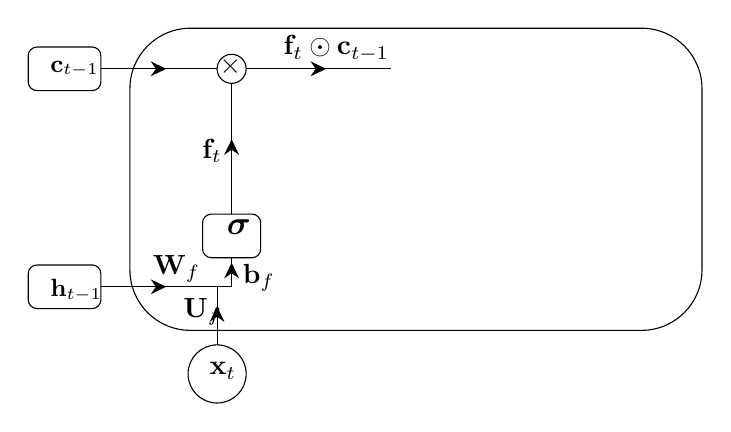
\begin{tikzpicture}[x=0.75pt,y=0.75pt,yscale=-0.7,xscale=0.7]
          %Shape: Ellipse [id:dp4969327327172295] 
          \draw   (160,280) .. controls (160,268.95) and (168.95,260) .. (180,260) .. controls (191.05,260) and (200,268.95) .. (200,280) .. controls (200,291.05) and (191.05,300) .. (180,300) .. controls (168.95,300) and (160,291.05) .. (160,280) -- cycle ;
          %Rounded Rect [id:dp8357991370192488] 
          \draw   (170,176) .. controls (170,172.69) and (172.69,170) .. (176,170) -- (204,170) .. controls (207.31,170) and (210,172.69) .. (210,176) -- (210,194) .. controls (210,197.31) and (207.31,200) .. (204,200) -- (176,200) .. controls (172.69,200) and (170,197.31) .. (170,194) -- cycle ;
          %Straight Lines [id:da3600219657240744] 
          \draw    (100,220) -- (180,220) ;
          \draw [shift={(145,220)}, rotate = 180] [fill={rgb, 255:red, 0; green, 0; blue, 0 }  ][line width=0.08]  [draw opacity=0] (10.72,-5.15) -- (0,0) -- (10.72,5.15) -- (7.12,0) -- cycle    ;
          %Rounded Rect [id:dp915587451603912] 
          \draw   (50,211) .. controls (50,207.69) and (52.69,205) .. (56,205) -- (94,205) .. controls (97.31,205) and (100,207.69) .. (100,211) -- (100,229) .. controls (100,232.31) and (97.31,235) .. (94,235) -- (56,235) .. controls (52.69,235) and (50,232.31) .. (50,229) -- cycle ;
          %Straight Lines [id:da9272238333173219] 
          \draw    (190,200) -- (190,220) ;
          \draw [shift={(190,203.5)}, rotate = 90] [fill={rgb, 255:red, 0; green, 0; blue, 0 }  ][line width=0.08]  [draw opacity=0] (10.72,-5.15) -- (0,0) -- (10.72,5.15) -- (7.12,0) -- cycle    ;
          %Straight Lines [id:da7830623178958898] 
          \draw    (190,80) -- (190,170) ;
          \draw [shift={(190,118.5)}, rotate = 90] [fill={rgb, 255:red, 0; green, 0; blue, 0 }  ][line width=0.08]  [draw opacity=0] (10.72,-5.15) -- (0,0) -- (10.72,5.15) -- (7.12,0) -- cycle    ;
          %Straight Lines [id:da008261007079938487] 
          \draw    (180,220) -- (180,260) ;
          \draw [shift={(180,233.5)}, rotate = 90] [fill={rgb, 255:red, 0; green, 0; blue, 0 }  ][line width=0.08]  [draw opacity=0] (10.72,-5.15) -- (0,0) -- (10.72,5.15) -- (7.12,0) -- cycle    ;
          %Straight Lines [id:da6327623101696669] 
          \draw    (180,220) -- (190,220) ;
          %Rounded Rect [id:dp1558027289731856] 
          \draw   (120,83.64) .. controls (120,60.67) and (138.62,42.05) .. (161.59,42.05) -- (472.14,42.05) .. controls (495.11,42.05) and (513.73,60.67) .. (513.73,83.64) -- (513.73,208.41) .. controls (513.73,231.38) and (495.11,250) .. (472.14,250) -- (161.59,250) .. controls (138.62,250) and (120,231.38) .. (120,208.41) -- cycle ;
          %Rounded Rect [id:dp3095760028615271] 
          \draw   (50,61) .. controls (50,57.69) and (52.69,55) .. (56,55) -- (94,55) .. controls (97.31,55) and (100,57.69) .. (100,61) -- (100,79) .. controls (100,82.31) and (97.31,85) .. (94,85) -- (56,85) .. controls (52.69,85) and (50,82.31) .. (50,79) -- cycle ;
          %Shape: Ellipse [id:dp04583613718786217] 
          \draw   (180,70) .. controls (180,64.48) and (184.48,60) .. (190,60) .. controls (195.52,60) and (200,64.48) .. (200,70) .. controls (200,75.52) and (195.52,80) .. (190,80) .. controls (184.48,80) and (180,75.52) .. (180,70) -- cycle ;
          %Straight Lines [id:da7337073083902665] 
          \draw    (100,70) -- (180,70) ;
          \draw [shift={(145,70)}, rotate = 180] [fill={rgb, 255:red, 0; green, 0; blue, 0 }  ][line width=0.08]  [draw opacity=0] (10.72,-5.15) -- (0,0) -- (10.72,5.15) -- (7.12,0) -- cycle    ;
          %Straight Lines [id:da19524926020736277] 
          \draw    (200,70) -- (300,70) ;
          \draw [shift={(255,70)}, rotate = 180] [fill={rgb, 255:red, 0; green, 0; blue, 0 }  ][line width=0.08]  [draw opacity=0] (10.72,-5.15) -- (0,0) -- (10.72,5.15) -- (7.12,0) -- cycle    ;

          % Text Node
          \draw (173,270.4) node [anchor=north west][inner sep=0.75pt]  [font=\normalsize]  {$\mathbf{x}_{t}$};
          % Text Node
          \draw (185,172.4) node [anchor=north west][inner sep=0.75pt]  [font=\large]  {$\boldsymbol{\sigma }$};
          % Text Node
          \draw (63.38,212.9) node [anchor=north west][inner sep=0.75pt]  [font=\small]  {$\mathbf{h}_{t-1}$};
          % Text Node
          \draw (168,116.4) node [anchor=north west][inner sep=0.75pt]  [font=\normalsize]  {$\mathbf{f}_{t}$};
          % Text Node
          \draw (224,45.4) node [anchor=north west][inner sep=0.75pt]  [font=\normalsize]  {$\mathbf{f}_{t} \odot \mathbf{c}_{t-1}$};
          % Text Node
          \draw (134,196.4) node [anchor=north west][inner sep=0.75pt]  [font=\normalsize]  {$\mathbf{W}_{f}$};
          % Text Node
          \draw (155,226.4) node [anchor=north west][inner sep=0.75pt]  [font=\normalsize]  {$\mathbf{U}_{f}$};
          % Text Node
          \draw (196,202.4) node [anchor=north west][inner sep=0.75pt]  [font=\normalsize]  {$\mathbf{b}_{f}$};
          % Text Node
          \draw (63.38,62.9) node [anchor=north west][inner sep=0.75pt]  [font=\small]  {$\mathbf{c}_{t-1}$};
          % Text Node
          \draw (180,60.4) node [anchor=north west][inner sep=0.75pt]  [font=\normalsize]  {$\times $};
        \end{tikzpicture}
        \caption{} 
        \label{fig:lstm_node_1}
      \end{figure}
      
      \item The \textbf{input gate} (denoted by $\mathbf{i}$) consists of two activations with the following operations. 
      \begin{align}
          \mathbf{i}_t & = \boldsymbol{\sigma}( \mathbf{W}_i \mathbf{h}_{t-1} + \mathbf{U}_i \mathbf{x}_t + \mathbf{b}_i ) \\
          \Tilde{\mathbf{c}}_t & = \boldsymbol{\tanh}( \mathbf{W}_c \mathbf{h}_{t-1} + \mathbf{U}_c \mathbf{x}_t + \mathbf{b}_c ) \\ 
          \mathbf{c}_t & = \mathbf{f}_t \odot \mathbf{c}_{t-1} + \mathbf{i}_t \odot \Tilde{\mathbf{c}}_t 
      \end{align}

      The layer $\mathbf{i}$ can be seen as the filter that selects which information can pass through it and what information to be discarded. To create this layer, we pass the short-term memory and current input into a sigmoid function, which will transform the values to be between $0$ and $1$, indicating which information is unimportant. The second layer $\Tilde{\mathbf{c}}$ takes the short term memory and current input and uses the $\tanh$ to transform the elements to be in $(-1, 1)$, which allows us to add or subtract the necessary information from the long term memory. 

      \begin{figure}[H]
        \centering 
        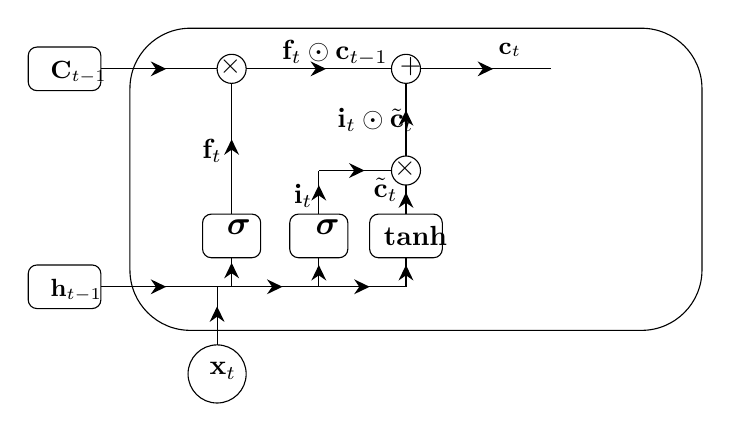
\begin{tikzpicture}[x=0.75pt,y=0.75pt,yscale=-0.7,xscale=0.7]
          %Shape: Ellipse [id:dp673856687206376] 
          \draw   (180,327.95) .. controls (180,316.91) and (188.95,307.95) .. (200,307.95) .. controls (211.05,307.95) and (220,316.91) .. (220,327.95) .. controls (220,339) and (211.05,347.95) .. (200,347.95) .. controls (188.95,347.95) and (180,339) .. (180,327.95) -- cycle ;
          %Rounded Rect [id:dp10309162377764869] 
          \draw   (190,223.95) .. controls (190,220.64) and (192.69,217.95) .. (196,217.95) -- (224,217.95) .. controls (227.31,217.95) and (230,220.64) .. (230,223.95) -- (230,241.95) .. controls (230,245.27) and (227.31,247.95) .. (224,247.95) -- (196,247.95) .. controls (192.69,247.95) and (190,245.27) .. (190,241.95) -- cycle ;
          %Straight Lines [id:da6240205957335716] 
          \draw    (120,267.95) -- (200,267.95) ;
          \draw [shift={(165,267.95)}, rotate = 180] [fill={rgb, 255:red, 0; green, 0; blue, 0 }  ][line width=0.08]  [draw opacity=0] (10.72,-5.15) -- (0,0) -- (10.72,5.15) -- (7.12,0) -- cycle    ;
          %Rounded Rect [id:dp6098888041343062] 
          \draw   (70,258.95) .. controls (70,255.64) and (72.69,252.95) .. (76,252.95) -- (114,252.95) .. controls (117.31,252.95) and (120,255.64) .. (120,258.95) -- (120,276.95) .. controls (120,280.27) and (117.31,282.95) .. (114,282.95) -- (76,282.95) .. controls (72.69,282.95) and (70,280.27) .. (70,276.95) -- cycle ;
          %Straight Lines [id:da6043978269854642] 
          \draw    (210,247.95) -- (210,267.95) ;
          \draw [shift={(210,251.45)}, rotate = 90] [fill={rgb, 255:red, 0; green, 0; blue, 0 }  ][line width=0.08]  [draw opacity=0] (10.72,-5.15) -- (0,0) -- (10.72,5.15) -- (7.12,0) -- cycle    ;
          %Straight Lines [id:da09325682821607639] 
          \draw    (210,127.95) -- (210,217.95) ;
          \draw [shift={(210,166.45)}, rotate = 90] [fill={rgb, 255:red, 0; green, 0; blue, 0 }  ][line width=0.08]  [draw opacity=0] (10.72,-5.15) -- (0,0) -- (10.72,5.15) -- (7.12,0) -- cycle    ;
          %Rounded Rect [id:dp605422940907552] 
          \draw   (250,223.95) .. controls (250,220.64) and (252.69,217.95) .. (256,217.95) -- (284,217.95) .. controls (287.31,217.95) and (290,220.64) .. (290,223.95) -- (290,241.95) .. controls (290,245.27) and (287.31,247.95) .. (284,247.95) -- (256,247.95) .. controls (252.69,247.95) and (250,245.27) .. (250,241.95) -- cycle ;
          %Straight Lines [id:da1280805304517283] 
          \draw    (200,267.95) -- (200,307.95) ;
          \draw [shift={(200,281.45)}, rotate = 90] [fill={rgb, 255:red, 0; green, 0; blue, 0 }  ][line width=0.08]  [draw opacity=0] (10.72,-5.15) -- (0,0) -- (10.72,5.15) -- (7.12,0) -- cycle    ;
          %Straight Lines [id:da34447299041881574] 
          \draw    (200,267.95) -- (210,267.95) ;
          %Straight Lines [id:da337875745538847] 
          \draw    (210,267.95) -- (270,267.95) ;
          \draw [shift={(245,267.95)}, rotate = 180] [fill={rgb, 255:red, 0; green, 0; blue, 0 }  ][line width=0.08]  [draw opacity=0] (10.72,-5.15) -- (0,0) -- (10.72,5.15) -- (7.12,0) -- cycle    ;
          %Rounded Rect [id:dp015328935957077405] 
          \draw   (305,223.95) .. controls (305,220.64) and (307.69,217.95) .. (311,217.95) -- (349,217.95) .. controls (352.31,217.95) and (355,220.64) .. (355,223.95) -- (355,241.95) .. controls (355,245.27) and (352.31,247.95) .. (349,247.95) -- (311,247.95) .. controls (307.69,247.95) and (305,245.27) .. (305,241.95) -- cycle ;
          %Straight Lines [id:da225547149220509] 
          \draw    (270,267.95) -- (270,247.95) ;
          \draw [shift={(270,252.95)}, rotate = 90] [fill={rgb, 255:red, 0; green, 0; blue, 0 }  ][line width=0.08]  [draw opacity=0] (10.72,-5.15) -- (0,0) -- (10.72,5.15) -- (7.12,0) -- cycle    ;
          %Straight Lines [id:da6795943289184077] 
          \draw    (330,267.95) -- (330,247.95) ;
          \draw [shift={(330,252.95)}, rotate = 90] [fill={rgb, 255:red, 0; green, 0; blue, 0 }  ][line width=0.08]  [draw opacity=0] (10.72,-5.15) -- (0,0) -- (10.72,5.15) -- (7.12,0) -- cycle    ;
          %Straight Lines [id:da21779293195502758] 
          \draw    (330,217.95) -- (330,197.95) ;
          \draw [shift={(330,202.95)}, rotate = 90] [fill={rgb, 255:red, 0; green, 0; blue, 0 }  ][line width=0.08]  [draw opacity=0] (10.72,-5.15) -- (0,0) -- (10.72,5.15) -- (7.12,0) -- cycle    ;
          %Straight Lines [id:da4764731211730844] 
          \draw    (270,217.95) -- (270,187.95) ;
          \draw [shift={(270,197.95)}, rotate = 90] [fill={rgb, 255:red, 0; green, 0; blue, 0 }  ][line width=0.08]  [draw opacity=0] (10.72,-5.15) -- (0,0) -- (10.72,5.15) -- (7.12,0) -- cycle    ;
          %Shape: Ellipse [id:dp38154006355076087] 
          \draw   (320,187.95) .. controls (320,182.43) and (324.48,177.95) .. (330,177.95) .. controls (335.52,177.95) and (340,182.43) .. (340,187.95) .. controls (340,193.48) and (335.52,197.95) .. (330,197.95) .. controls (324.48,197.95) and (320,193.48) .. (320,187.95) -- cycle ;
          %Straight Lines [id:da3258632871225313] 
          \draw    (320,187.95) -- (270,187.95) ;
          \draw [shift={(301.5,187.95)}, rotate = 180] [fill={rgb, 255:red, 0; green, 0; blue, 0 }  ][line width=0.08]  [draw opacity=0] (10.72,-5.15) -- (0,0) -- (10.72,5.15) -- (7.12,0) -- cycle    ;
          %Straight Lines [id:da5423947396221587] 
          \draw    (330,127.95) -- (330,177.95) ;
          \draw [shift={(330,146.45)}, rotate = 90] [fill={rgb, 255:red, 0; green, 0; blue, 0 }  ][line width=0.08]  [draw opacity=0] (10.72,-5.15) -- (0,0) -- (10.72,5.15) -- (7.12,0) -- cycle    ;
          %Straight Lines [id:da7595203590607811] 
          \draw    (270,267.95) -- (330,267.95) ;
          \draw [shift={(305,267.95)}, rotate = 180] [fill={rgb, 255:red, 0; green, 0; blue, 0 }  ][line width=0.08]  [draw opacity=0] (10.72,-5.15) -- (0,0) -- (10.72,5.15) -- (7.12,0) -- cycle    ;
          %Rounded Rect [id:dp998433719384372] 
          \draw   (140,131.59) .. controls (140,108.62) and (158.62,90) .. (181.59,90) -- (492.14,90) .. controls (515.11,90) and (533.73,108.62) .. (533.73,131.59) -- (533.73,256.36) .. controls (533.73,279.33) and (515.11,297.95) .. (492.14,297.95) -- (181.59,297.95) .. controls (158.62,297.95) and (140,279.33) .. (140,256.36) -- cycle ;
          %Rounded Rect [id:dp5009767130679297] 
          \draw   (70,108.95) .. controls (70,105.64) and (72.69,102.95) .. (76,102.95) -- (114,102.95) .. controls (117.31,102.95) and (120,105.64) .. (120,108.95) -- (120,126.95) .. controls (120,130.27) and (117.31,132.95) .. (114,132.95) -- (76,132.95) .. controls (72.69,132.95) and (70,130.27) .. (70,126.95) -- cycle ;
          %Shape: Ellipse [id:dp5406765889795262] 
          \draw   (200,117.95) .. controls (200,112.43) and (204.48,107.95) .. (210,107.95) .. controls (215.52,107.95) and (220,112.43) .. (220,117.95) .. controls (220,123.48) and (215.52,127.95) .. (210,127.95) .. controls (204.48,127.95) and (200,123.48) .. (200,117.95) -- cycle ;
          %Straight Lines [id:da2940801686510699] 
          \draw    (120,117.95) -- (200,117.95) ;
          \draw [shift={(165,117.95)}, rotate = 180] [fill={rgb, 255:red, 0; green, 0; blue, 0 }  ][line width=0.08]  [draw opacity=0] (10.72,-5.15) -- (0,0) -- (10.72,5.15) -- (7.12,0) -- cycle    ;
          %Straight Lines [id:da047556376575517145] 
          \draw    (220,117.95) -- (320,117.95) ;
          \draw [shift={(275,117.95)}, rotate = 180] [fill={rgb, 255:red, 0; green, 0; blue, 0 }  ][line width=0.08]  [draw opacity=0] (10.72,-5.15) -- (0,0) -- (10.72,5.15) -- (7.12,0) -- cycle    ;
          %Shape: Ellipse [id:dp004236969372855448] 
          \draw   (320,117.95) .. controls (320,112.43) and (324.48,107.95) .. (330,107.95) .. controls (335.52,107.95) and (340,112.43) .. (340,117.95) .. controls (340,123.48) and (335.52,127.95) .. (330,127.95) .. controls (324.48,127.95) and (320,123.48) .. (320,117.95) -- cycle ;
          %Straight Lines [id:da42944638467678886] 
          \draw    (340,117.95) -- (430,117.95) ;
          \draw [shift={(390,117.95)}, rotate = 180] [fill={rgb, 255:red, 0; green, 0; blue, 0 }  ][line width=0.08]  [draw opacity=0] (10.72,-5.15) -- (0,0) -- (10.72,5.15) -- (7.12,0) -- cycle    ;

          % Text Node
          \draw (193,318.35) node [anchor=north west][inner sep=0.75pt]  [font=\normalsize]  {$\mathbf{x}_{t}$};
          % Text Node
          \draw (205,220.35) node [anchor=north west][inner sep=0.75pt]  [font=\large]  {$\boldsymbol{\sigma }$};
          % Text Node
          \draw (83.38,260.85) node [anchor=north west][inner sep=0.75pt]  [font=\small]  {$\mathbf{h}_{t-1}$};
          % Text Node
          \draw (266,220.35) node [anchor=north west][inner sep=0.75pt]  [font=\large]  {$\boldsymbol{\sigma }$};
          % Text Node
          \draw (188,164.35) node [anchor=north west][inner sep=0.75pt]  [font=\normalsize]  {$\mathbf{f}_{t}$};
          % Text Node
          \draw (313,224.35) node [anchor=north west][inner sep=0.75pt]  [font=\normalsize]  {$\mathbf{tanh}$};
          % Text Node
          \draw (320,178.35) node [anchor=north west][inner sep=0.75pt]  [font=\normalsize]  {$\times $};
          % Text Node
          \draw (83.38,110.85) node [anchor=north west][inner sep=0.75pt]  [font=\small]  {$\mathbf{C}_{t-1}$};
          % Text Node
          \draw (200,108.35) node [anchor=north west][inner sep=0.75pt]  [font=\normalsize]  {$\times $};
          % Text Node
          \draw (324,108.35) node [anchor=north west][inner sep=0.75pt]  [font=\normalsize]  {$+$};
          % Text Node
          \draw (251,195.4) node [anchor=north west][inner sep=0.75pt]  [font=\normalsize]  {$\mathbf{i}_{t}$};
          % Text Node
          \draw (306,191.4) node [anchor=north west][inner sep=0.75pt]  [font=\normalsize]  {$\tilde{\mathbf{c}}_{t}$};
          % Text Node
          \draw (243,96.4) node [anchor=north west][inner sep=0.75pt]  [font=\normalsize]  {$\mathbf{f}_{t} \odot \mathbf{c}_{t-1}$};
          % Text Node
          \draw (281,143.4) node [anchor=north west][inner sep=0.75pt]  [font=\normalsize]  {$\mathbf{i}_{t} \odot \tilde{\mathbf{c}}_{t}$};
          % Text Node
          \draw (392,98.4) node [anchor=north west][inner sep=0.75pt]  [font=\small]  {$\mathbf{c}_{t}$};
        \end{tikzpicture}
        \caption{} 
        \label{fig:lstm_node_2}
      \end{figure}

      \item The \textbf{output gate} (denoted by $\mathbf{o}$) consists of two activations with the following operations. This again creates a separate filter that selects the relevant information needed for the short term memory. 
      \begin{align}
          \mathbf{o}_t & = \boldsymbol{\sigma}( \mathbf{W}_o \mathbf{h}_{t-1} + \mathbf{U}_o \mathbf{x}_t + \mathbf{b}_o ) \\
          \mathbf{h}_t & = \mathbf{o}_t \odot \boldsymbol{\tanh}(\mathbf{c}_t) \\
          \hat{\mathbf{y}}_t & = \boldsymbol{\sigma}_y ( \mathbf{V} \mathbf{h}_t + \mathbf{b}_y)
      \end{align}

      \begin{figure}[H]
        \centering 
        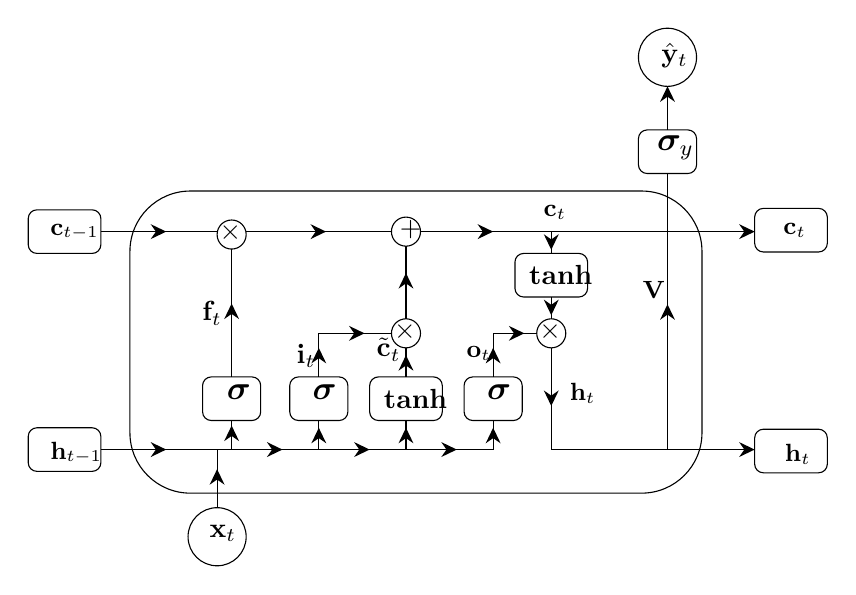
\begin{tikzpicture}[x=0.75pt,y=0.75pt,yscale=-0.7,xscale=0.7]
          %Rounded Rect [id:dp7607307729058677] 
          \draw   (140,163.64) .. controls (140,140.67) and (158.62,122.05) .. (181.59,122.05) -- (492.14,122.05) .. controls (515.11,122.05) and (533.73,140.67) .. (533.73,163.64) -- (533.73,288.41) .. controls (533.73,311.38) and (515.11,330) .. (492.14,330) -- (181.59,330) .. controls (158.62,330) and (140,311.38) .. (140,288.41) -- cycle ;
          %Shape: Ellipse [id:dp900217564752672] 
          \draw   (180,360) .. controls (180,348.95) and (188.95,340) .. (200,340) .. controls (211.05,340) and (220,348.95) .. (220,360) .. controls (220,371.05) and (211.05,380) .. (200,380) .. controls (188.95,380) and (180,371.05) .. (180,360) -- cycle ;
          %Rounded Rect [id:dp6893065668366456] 
          \draw   (190,256) .. controls (190,252.69) and (192.69,250) .. (196,250) -- (224,250) .. controls (227.31,250) and (230,252.69) .. (230,256) -- (230,274) .. controls (230,277.31) and (227.31,280) .. (224,280) -- (196,280) .. controls (192.69,280) and (190,277.31) .. (190,274) -- cycle ;
          %Straight Lines [id:da5343888843478] 
          \draw    (120,300) -- (200,300) ;
          \draw [shift={(165,300)}, rotate = 180] [fill={rgb, 255:red, 0; green, 0; blue, 0 }  ][line width=0.08]  [draw opacity=0] (10.72,-5.15) -- (0,0) -- (10.72,5.15) -- (7.12,0) -- cycle    ;
          %Rounded Rect [id:dp16398311464764093] 
          \draw   (70,291) .. controls (70,287.69) and (72.69,285) .. (76,285) -- (114,285) .. controls (117.31,285) and (120,287.69) .. (120,291) -- (120,309) .. controls (120,312.31) and (117.31,315) .. (114,315) -- (76,315) .. controls (72.69,315) and (70,312.31) .. (70,309) -- cycle ;
          %Rounded Rect [id:dp7552509756915937] 
          \draw   (70,141) .. controls (70,137.69) and (72.69,135) .. (76,135) -- (114,135) .. controls (117.31,135) and (120,137.69) .. (120,141) -- (120,159) .. controls (120,162.31) and (117.31,165) .. (114,165) -- (76,165) .. controls (72.69,165) and (70,162.31) .. (70,159) -- cycle ;
          %Straight Lines [id:da304843264938752] 
          \draw    (210,280) -- (210,300) ;
          \draw [shift={(210,283.5)}, rotate = 90] [fill={rgb, 255:red, 0; green, 0; blue, 0 }  ][line width=0.08]  [draw opacity=0] (10.72,-5.15) -- (0,0) -- (10.72,5.15) -- (7.12,0) -- cycle    ;
          %Straight Lines [id:da14284118067632345] 
          \draw    (210,162) -- (210,250) ;
          \draw [shift={(210,199.5)}, rotate = 90] [fill={rgb, 255:red, 0; green, 0; blue, 0 }  ][line width=0.08]  [draw opacity=0] (10.72,-5.15) -- (0,0) -- (10.72,5.15) -- (7.12,0) -- cycle    ;
          %Shape: Ellipse [id:dp5396089408185574] 
          \draw   (200,152) .. controls (200,146.48) and (204.48,142) .. (210,142) .. controls (215.52,142) and (220,146.48) .. (220,152) .. controls (220,157.52) and (215.52,162) .. (210,162) .. controls (204.48,162) and (200,157.52) .. (200,152) -- cycle ;
          %Straight Lines [id:da9933430333496693] 
          \draw    (120,150) -- (200,150) ;
          \draw [shift={(165,150)}, rotate = 180] [fill={rgb, 255:red, 0; green, 0; blue, 0 }  ][line width=0.08]  [draw opacity=0] (10.72,-5.15) -- (0,0) -- (10.72,5.15) -- (7.12,0) -- cycle    ;
          %Straight Lines [id:da8940095383250102] 
          \draw    (220,150) -- (320,150) ;
          \draw [shift={(275,150)}, rotate = 180] [fill={rgb, 255:red, 0; green, 0; blue, 0 }  ][line width=0.08]  [draw opacity=0] (10.72,-5.15) -- (0,0) -- (10.72,5.15) -- (7.12,0) -- cycle    ;
          %Rounded Rect [id:dp25314537917502555] 
          \draw   (250,256) .. controls (250,252.69) and (252.69,250) .. (256,250) -- (284,250) .. controls (287.31,250) and (290,252.69) .. (290,256) -- (290,274) .. controls (290,277.31) and (287.31,280) .. (284,280) -- (256,280) .. controls (252.69,280) and (250,277.31) .. (250,274) -- cycle ;
          %Straight Lines [id:da7871629509904587] 
          \draw    (200,300) -- (200,340) ;
          \draw [shift={(200,313.5)}, rotate = 90] [fill={rgb, 255:red, 0; green, 0; blue, 0 }  ][line width=0.08]  [draw opacity=0] (10.72,-5.15) -- (0,0) -- (10.72,5.15) -- (7.12,0) -- cycle    ;
          %Straight Lines [id:da1940620806488591] 
          \draw    (200,300) -- (210,300) ;
          %Straight Lines [id:da5912482065359186] 
          \draw    (210,300) -- (270,300) ;
          \draw [shift={(245,300)}, rotate = 180] [fill={rgb, 255:red, 0; green, 0; blue, 0 }  ][line width=0.08]  [draw opacity=0] (10.72,-5.15) -- (0,0) -- (10.72,5.15) -- (7.12,0) -- cycle    ;
          %Shape: Ellipse [id:dp4841686324219643] 
          \draw   (320,150) .. controls (320,144.48) and (324.48,140) .. (330,140) .. controls (335.52,140) and (340,144.48) .. (340,150) .. controls (340,155.52) and (335.52,160) .. (330,160) .. controls (324.48,160) and (320,155.52) .. (320,150) -- cycle ;
          %Rounded Rect [id:dp31865438690386094] 
          \draw   (305,256) .. controls (305,252.69) and (307.69,250) .. (311,250) -- (349,250) .. controls (352.31,250) and (355,252.69) .. (355,256) -- (355,274) .. controls (355,277.31) and (352.31,280) .. (349,280) -- (311,280) .. controls (307.69,280) and (305,277.31) .. (305,274) -- cycle ;
          %Straight Lines [id:da5645041143915148] 
          \draw    (270,300) -- (270,280) ;
          \draw [shift={(270,285)}, rotate = 90] [fill={rgb, 255:red, 0; green, 0; blue, 0 }  ][line width=0.08]  [draw opacity=0] (10.72,-5.15) -- (0,0) -- (10.72,5.15) -- (7.12,0) -- cycle    ;
          %Straight Lines [id:da9431818949019313] 
          \draw    (330,300) -- (330,280) ;
          \draw [shift={(330,285)}, rotate = 90] [fill={rgb, 255:red, 0; green, 0; blue, 0 }  ][line width=0.08]  [draw opacity=0] (10.72,-5.15) -- (0,0) -- (10.72,5.15) -- (7.12,0) -- cycle    ;
          %Straight Lines [id:da11777621499218438] 
          \draw    (330,250) -- (330,230) ;
          \draw [shift={(330,235)}, rotate = 90] [fill={rgb, 255:red, 0; green, 0; blue, 0 }  ][line width=0.08]  [draw opacity=0] (10.72,-5.15) -- (0,0) -- (10.72,5.15) -- (7.12,0) -- cycle    ;
          %Straight Lines [id:da9724379887976446] 
          \draw    (270,250) -- (270,220) ;
          \draw [shift={(270,230)}, rotate = 90] [fill={rgb, 255:red, 0; green, 0; blue, 0 }  ][line width=0.08]  [draw opacity=0] (10.72,-5.15) -- (0,0) -- (10.72,5.15) -- (7.12,0) -- cycle    ;
          %Shape: Ellipse [id:dp6921024732199978] 
          \draw   (320,220) .. controls (320,214.48) and (324.48,210) .. (330,210) .. controls (335.52,210) and (340,214.48) .. (340,220) .. controls (340,225.52) and (335.52,230) .. (330,230) .. controls (324.48,230) and (320,225.52) .. (320,220) -- cycle ;
          %Straight Lines [id:da1410394226097551] 
          \draw    (320,220) -- (270,220) ;
          \draw [shift={(301.5,220)}, rotate = 180] [fill={rgb, 255:red, 0; green, 0; blue, 0 }  ][line width=0.08]  [draw opacity=0] (10.72,-5.15) -- (0,0) -- (10.72,5.15) -- (7.12,0) -- cycle    ;
          %Straight Lines [id:da4451936356762698] 
          \draw    (330,160) -- (330,210) ;
          \draw [shift={(330,178.5)}, rotate = 90] [fill={rgb, 255:red, 0; green, 0; blue, 0 }  ][line width=0.08]  [draw opacity=0] (10.72,-5.15) -- (0,0) -- (10.72,5.15) -- (7.12,0) -- cycle    ;
          %Straight Lines [id:da8250107200889327] 
          \draw    (270,300) -- (330,300) ;
          \draw [shift={(305,300)}, rotate = 180] [fill={rgb, 255:red, 0; green, 0; blue, 0 }  ][line width=0.08]  [draw opacity=0] (10.72,-5.15) -- (0,0) -- (10.72,5.15) -- (7.12,0) -- cycle    ;
          %Straight Lines [id:da31368624536525] 
          \draw    (340,150) -- (430,150) ;
          \draw [shift={(390,150)}, rotate = 180] [fill={rgb, 255:red, 0; green, 0; blue, 0 }  ][line width=0.08]  [draw opacity=0] (10.72,-5.15) -- (0,0) -- (10.72,5.15) -- (7.12,0) -- cycle    ;
          %Straight Lines [id:da680791431454264] 
          \draw    (330,300) -- (390,300) ;
          \draw [shift={(365,300)}, rotate = 180] [fill={rgb, 255:red, 0; green, 0; blue, 0 }  ][line width=0.08]  [draw opacity=0] (10.72,-5.15) -- (0,0) -- (10.72,5.15) -- (7.12,0) -- cycle    ;
          %Rounded Rect [id:dp4093507732748505] 
          \draw   (370,256) .. controls (370,252.69) and (372.69,250) .. (376,250) -- (404,250) .. controls (407.31,250) and (410,252.69) .. (410,256) -- (410,274) .. controls (410,277.31) and (407.31,280) .. (404,280) -- (376,280) .. controls (372.69,280) and (370,277.31) .. (370,274) -- cycle ;
          %Straight Lines [id:da05493337879481186] 
          \draw    (390,300) -- (390,280) ;
          \draw [shift={(390,285)}, rotate = 90] [fill={rgb, 255:red, 0; green, 0; blue, 0 }  ][line width=0.08]  [draw opacity=0] (10.72,-5.15) -- (0,0) -- (10.72,5.15) -- (7.12,0) -- cycle    ;
          %Straight Lines [id:da2852801639207645] 
          \draw    (390,250) -- (390,220) ;
          \draw [shift={(390,230)}, rotate = 90] [fill={rgb, 255:red, 0; green, 0; blue, 0 }  ][line width=0.08]  [draw opacity=0] (10.72,-5.15) -- (0,0) -- (10.72,5.15) -- (7.12,0) -- cycle    ;
          %Straight Lines [id:da10205317474403763] 
          \draw    (420,220) -- (390,220) ;
          \draw [shift={(411.5,220)}, rotate = 180] [fill={rgb, 255:red, 0; green, 0; blue, 0 }  ][line width=0.08]  [draw opacity=0] (10.72,-5.15) -- (0,0) -- (10.72,5.15) -- (7.12,0) -- cycle    ;
          %Shape: Ellipse [id:dp656470469132832] 
          \draw   (420,220) .. controls (420,214.48) and (424.48,210) .. (430,210) .. controls (435.52,210) and (440,214.48) .. (440,220) .. controls (440,225.52) and (435.52,230) .. (430,230) .. controls (424.48,230) and (420,225.52) .. (420,220) -- cycle ;
          %Rounded Rect [id:dp7702057134779456] 
          \draw   (405,171) .. controls (405,167.69) and (407.69,165) .. (411,165) -- (449,165) .. controls (452.31,165) and (455,167.69) .. (455,171) -- (455,189) .. controls (455,192.31) and (452.31,195) .. (449,195) -- (411,195) .. controls (407.69,195) and (405,192.31) .. (405,189) -- cycle ;
          %Straight Lines [id:da06612853990545564] 
          \draw    (430,150) -- (430,165) ;
          \draw [shift={(430,162.5)}, rotate = 270] [fill={rgb, 255:red, 0; green, 0; blue, 0 }  ][line width=0.08]  [draw opacity=0] (10.72,-5.15) -- (0,0) -- (10.72,5.15) -- (7.12,0) -- cycle    ;
          %Straight Lines [id:da9855082148874492] 
          \draw    (430,195) -- (430,210) ;
          \draw [shift={(430,207.5)}, rotate = 270] [fill={rgb, 255:red, 0; green, 0; blue, 0 }  ][line width=0.08]  [draw opacity=0] (10.72,-5.15) -- (0,0) -- (10.72,5.15) -- (7.12,0) -- cycle    ;
          %Straight Lines [id:da6917168175796875] 
          \draw    (430,150) -- (567,150) ;
          \draw [shift={(570,150)}, rotate = 180] [fill={rgb, 255:red, 0; green, 0; blue, 0 }  ][line width=0.08]  [draw opacity=0] (10.72,-5.15) -- (0,0) -- (10.72,5.15) -- (7.12,0) -- cycle    ;
          %Rounded Rect [id:dp7717143285394976] 
          \draw   (570,140) .. controls (570,136.69) and (572.69,134) .. (576,134) -- (614,134) .. controls (617.31,134) and (620,136.69) .. (620,140) -- (620,158) .. controls (620,161.31) and (617.31,164) .. (614,164) -- (576,164) .. controls (572.69,164) and (570,161.31) .. (570,158) -- cycle ;
          %Straight Lines [id:da9058130105060662] 
          \draw    (430,230) -- (430,300) ;
          \draw [shift={(430,270)}, rotate = 270] [fill={rgb, 255:red, 0; green, 0; blue, 0 }  ][line width=0.08]  [draw opacity=0] (10.72,-5.15) -- (0,0) -- (10.72,5.15) -- (7.12,0) -- cycle    ;
          %Straight Lines [id:da40006208395694376] 
          \draw    (430,300) -- (567,300) ;
          \draw [shift={(570,300)}, rotate = 180] [fill={rgb, 255:red, 0; green, 0; blue, 0 }  ][line width=0.08]  [draw opacity=0] (10.72,-5.15) -- (0,0) -- (10.72,5.15) -- (7.12,0) -- cycle    ;
          %Rounded Rect [id:dp8925711851370559] 
          \draw   (570,292) .. controls (570,288.69) and (572.69,286) .. (576,286) -- (614,286) .. controls (617.31,286) and (620,288.69) .. (620,292) -- (620,310) .. controls (620,313.31) and (617.31,316) .. (614,316) -- (576,316) .. controls (572.69,316) and (570,313.31) .. (570,310) -- cycle ;
          %Straight Lines [id:da3431993487488634] 
          \draw    (510,300) -- (510,110) ;
          \draw [shift={(510,200)}, rotate = 90] [fill={rgb, 255:red, 0; green, 0; blue, 0 }  ][line width=0.08]  [draw opacity=0] (10.72,-5.15) -- (0,0) -- (10.72,5.15) -- (7.12,0) -- cycle    ;
          %Shape: Ellipse [id:dp5223810693241391] 
          \draw   (490,30) .. controls (490,18.95) and (498.95,10) .. (510,10) .. controls (521.05,10) and (530,18.95) .. (530,30) .. controls (530,41.05) and (521.05,50) .. (510,50) .. controls (498.95,50) and (490,41.05) .. (490,30) -- cycle ;
          %Rounded Rect [id:dp08850756436330398] 
          \draw   (490,86) .. controls (490,82.69) and (492.69,80) .. (496,80) -- (524,80) .. controls (527.31,80) and (530,82.69) .. (530,86) -- (530,104) .. controls (530,107.31) and (527.31,110) .. (524,110) -- (496,110) .. controls (492.69,110) and (490,107.31) .. (490,104) -- cycle ;
          %Straight Lines [id:da8380296553480746] 
          \draw    (510,80) -- (510,53) ;
          \draw [shift={(510,50)}, rotate = 90] [fill={rgb, 255:red, 0; green, 0; blue, 0 }  ][line width=0.08]  [draw opacity=0] (10.72,-5.15) -- (0,0) -- (10.72,5.15) -- (7.12,0) -- cycle    ;

          % Text Node
          \draw (193,350.4) node [anchor=north west][inner sep=0.75pt]  [font=\normalsize]  {$\mathbf{x}_{t}$};
          % Text Node
          \draw (205,253.4) node [anchor=north west][inner sep=0.75pt]  [font=\large]  {$\boldsymbol{\sigma }$};
          % Text Node
          \draw (83.38,292.9) node [anchor=north west][inner sep=0.75pt]  [font=\small]  {$\mathbf{h}_{t-1}$};
          % Text Node
          \draw (83.38,142.9) node [anchor=north west][inner sep=0.75pt]  [font=\small]  {$\mathbf{c}_{t-1}$};
          % Text Node
          \draw (200,142.4) node [anchor=north west][inner sep=0.75pt]  [font=\normalsize]  {$\times $};
          % Text Node
          \draw (264,253.4) node [anchor=north west][inner sep=0.75pt]  [font=\large]  {$\boldsymbol{\sigma }$};
          % Text Node
          \draw (188,196.4) node [anchor=north west][inner sep=0.75pt]  [font=\normalsize]  {$\mathbf{f}_{t}$};
          % Text Node
          \draw (324,140.4) node [anchor=north west][inner sep=0.75pt]  [font=\normalsize]  {$+$};
          % Text Node
          \draw (313,256.4) node [anchor=north west][inner sep=0.75pt]  [font=\normalsize]  {$\mathbf{tanh}$};
          % Text Node
          \draw (320,210.4) node [anchor=north west][inner sep=0.75pt]  [font=\normalsize]  {$\times $};
          % Text Node
          \draw (384,253.4) node [anchor=north west][inner sep=0.75pt]  [font=\large]  {$\boldsymbol{\sigma }$};
          % Text Node
          \draw (420,210.4) node [anchor=north west][inner sep=0.75pt]  [font=\normalsize]  {$\times $};
          % Text Node
          \draw (413,171.4) node [anchor=north west][inner sep=0.75pt]  [font=\normalsize]  {$\mathbf{tanh}$};
          % Text Node
          \draw (588,142.4) node [anchor=north west][inner sep=0.75pt]  [font=\small]  {$\mathbf{c}_{t}$};
          % Text Node
          \draw (589,294.4) node [anchor=north west][inner sep=0.75pt]  [font=\small]  {$\mathbf{h}_{t}$};
          % Text Node
          \draw (504,18.4) node [anchor=north west][inner sep=0.75pt]  [font=\normalsize]  {$\hat{\mathbf{y}}_{t}$};
          % Text Node
          \draw (423,130.4) node [anchor=north west][inner sep=0.75pt]  [font=\small]  {$\mathbf{c}_{t}$};
          % Text Node
          \draw (370,227.4) node [anchor=north west][inner sep=0.75pt]  [font=\small]  {$\mathbf{o}_{t}$};
          % Text Node
          \draw (441,252.4) node [anchor=north west][inner sep=0.75pt]  [font=\small]  {$\mathbf{h}_{t}$};
          % Text Node
          \draw (501,82.4) node [anchor=north west][inner sep=0.75pt]  [font=\large]  {$\boldsymbol{\sigma }_{y}$};
          % Text Node
          \draw (491,182.4) node [anchor=north west][inner sep=0.75pt]  [font=\small]  {$\mathbf{V}$};
          % Text Node
          \draw (253,225.4) node [anchor=north west][inner sep=0.75pt]  [font=\normalsize]  {$\mathbf{i}_{t}$};
          % Text Node
          \draw (308,221.4) node [anchor=north west][inner sep=0.75pt]  [font=\normalsize]  {$\tilde{\mathbf{c}}_{t}$};
        \end{tikzpicture}
        \caption{} 
        \label{fig:lstm_node_3}
      \end{figure}
  \end{enumerate}
  That is it! Now focusing on the cell state in the diagram above. Note that in order to go from cell state $\mathbf{c}_{t-1}$ to $\mathbf{c}_t$, there was not a whole lot done to it. We really just multiply it once, which potentially deletes some content, and add it once, which adds new content, and we are done. The magic is this addition, since unlike multiplication, which can result in an exponential decay of knowledge, you are just constantly adding new numbers to update the storage, allowing the cell state to behave much more like RAM of a computer. 

  The LSTM architecture also makes it easier for the RNN to preserve information over many timesteps. For example, if the forget gate $\mathbf{f}_t$ is set to $\mathbf{1}$ and the input gate set to $\mathbf{0}$, then the information of that cell is preserved indefinitely. In contrast, it's harder for a vanilla RNN to learn a recurrent weight matrix $\mathbf{W}$ that preserves information in the hidden state. In practice, a vanilla RNN would preserve memory up to maybe 7 timesteps (and increasing this is extremely difficult) while a LSTM would get about 100 timesteps, so in practice you should almost always just use a LSTM. 

  Unfortunately, LSTM doesn't \textit{guarantee} that there is no vanishing or exploding gradients, but it does provide an easier way for the model to learn long-distance dependencies. Note that the gradient problem is not just a problem for RNNs; any neural architecture (including a feed-forward or convolutional) with very deep layers with multiple compositions of functions may suffer. Due to the chain rule and choice of nonlinearity function, these gradients can become vanishingly small and lower layers are learned very slowly. However, we can still implement residual connections to allow for more gradient flow such as ResNet, DenseNet, and HighwayNet. 

  \subsubsection{Multilayer LSTMs}

    We can extend this architecture in the exactly same way for multilayer LSTMs. Note that we should be careful of the transformations each arrow represents. For the arrows going from $\mathbf{h}_{t}^{[l]} \mapsto \mathbf{h}_{t}^{[l+1]}$, there is no further transformation since we are just pushing this vector as an input to the next LSTM node. However, the arrow pushing from $\mathbf{c}_t^{[L]} \mapsto \hat{\mathbf{y}}_{t}$ does have an extra affine transformation with $\mathbf{V}$ and $\mathbf{b}_y$, followed by some link function $\boldsymbol{\sigma}_y$ before we have the true prediction.  

    \begin{figure}[H]
      \centering 
      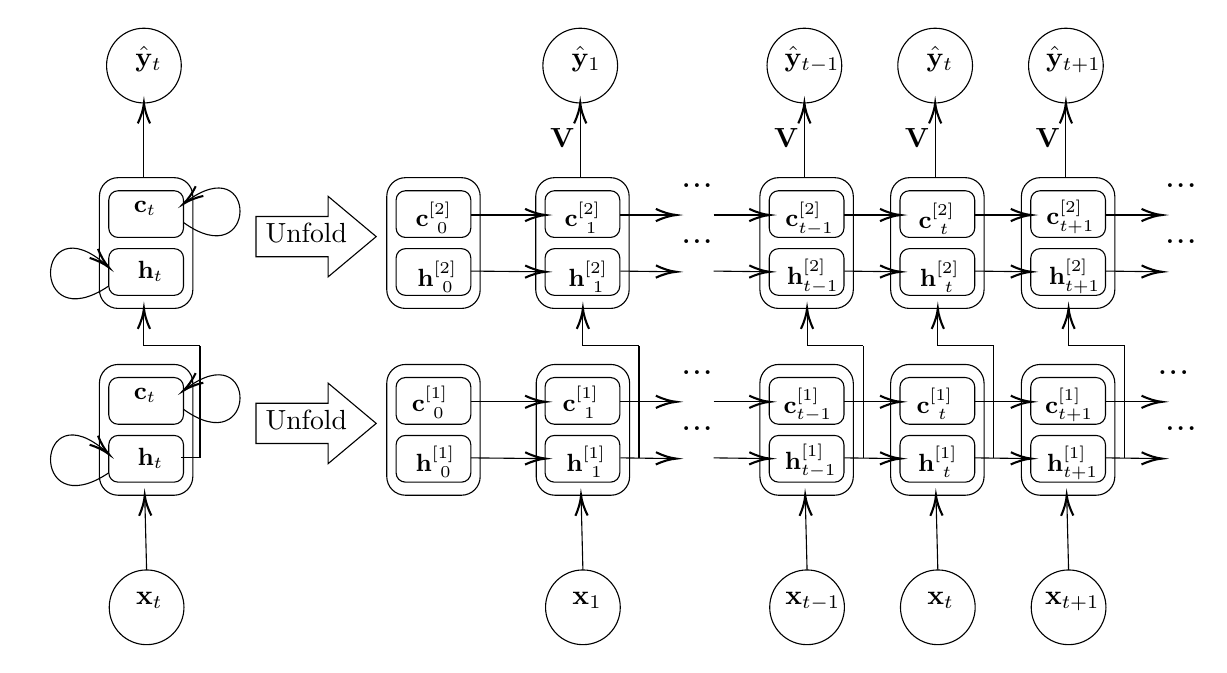
\begin{tikzpicture}[x=0.75pt,y=0.75pt,yscale=-0.9,xscale=0.9]
        %Rounded Rect [id:dp1729121626387391] 
        \draw   (51.18,200) .. controls (51.18,194.48) and (55.66,190) .. (61.18,190) -- (91.18,190) .. controls (96.71,190) and (101.18,194.48) .. (101.18,200) -- (101.18,250) .. controls (101.18,255.52) and (96.71,260) .. (91.18,260) -- (61.18,260) .. controls (55.66,260) and (51.18,255.52) .. (51.18,250) -- cycle ;
        %Rounded Rect [id:dp6162380210016798] 
        \draw   (56.18,202) .. controls (56.18,199.24) and (58.42,197) .. (61.18,197) -- (91.18,197) .. controls (93.95,197) and (96.18,199.24) .. (96.18,202) -- (96.18,217) .. controls (96.18,219.76) and (93.95,222) .. (91.18,222) -- (61.18,222) .. controls (58.42,222) and (56.18,219.76) .. (56.18,217) -- cycle ;
        %Rounded Rect [id:dp10367639876664736] 
        \draw   (56.18,233) .. controls (56.18,230.24) and (58.42,228) .. (61.18,228) -- (91.18,228) .. controls (93.95,228) and (96.18,230.24) .. (96.18,233) -- (96.18,248) .. controls (96.18,250.76) and (93.95,253) .. (91.18,253) -- (61.18,253) .. controls (58.42,253) and (56.18,250.76) .. (56.18,248) -- cycle ;
        %Curve Lines [id:da20240529841221622] 
        \draw [color={rgb, 255:red, 0; green, 0; blue, 0 }  ,draw opacity=1 ]   (96.18,214) .. controls (136.11,242.71) and (136.51,173.41) .. (97.38,203.07) ;
        \draw [shift={(96.18,204)}, rotate = 321.57] [color={rgb, 255:red, 0; green, 0; blue, 0 }  ,draw opacity=1 ][line width=0.75]    (10.93,-3.29) .. controls (6.95,-1.4) and (3.31,-0.3) .. (0,0) .. controls (3.31,0.3) and (6.95,1.4) .. (10.93,3.29)   ;
        %Curve Lines [id:da631199065967021] 
        \draw [color={rgb, 255:red, 0; green, 0; blue, 0 }  ,draw opacity=1 ]   (56.18,248) .. controls (13.06,276.93) and (16.55,202.73) .. (55.01,236.93) ;
        \draw [shift={(56.18,238)}, rotate = 222.92] [color={rgb, 255:red, 0; green, 0; blue, 0 }  ,draw opacity=1 ][line width=0.75]    (10.93,-3.29) .. controls (6.95,-1.4) and (3.31,-0.3) .. (0,0) .. controls (3.31,0.3) and (6.95,1.4) .. (10.93,3.29)   ;
        %Shape: Ellipse [id:dp3395210228264245] 
        \draw   (55,30) .. controls (55,18.95) and (63.95,10) .. (75,10) .. controls (86.05,10) and (95,18.95) .. (95,30) .. controls (95,41.05) and (86.05,50) .. (75,50) .. controls (63.95,50) and (55,41.05) .. (55,30) -- cycle ;
        %Straight Lines [id:da17924855399151696] 
        \draw [color={rgb, 255:red, 0; green, 0; blue, 0 }  ,draw opacity=1 ]   (75,90) -- (75,56) -- (75,52) ;
        \draw [shift={(75,50)}, rotate = 90] [color={rgb, 255:red, 0; green, 0; blue, 0 }  ,draw opacity=1 ][line width=0.75]    (10.93,-3.29) .. controls (6.95,-1.4) and (3.31,-0.3) .. (0,0) .. controls (3.31,0.3) and (6.95,1.4) .. (10.93,3.29)   ;
        %Shape: Ellipse [id:dp35088397695352525] 
        \draw   (56.43,320) .. controls (56.43,308.95) and (65.39,300) .. (76.43,300) .. controls (87.48,300) and (96.43,308.95) .. (96.43,320) .. controls (96.43,331.05) and (87.48,340) .. (76.43,340) .. controls (65.39,340) and (56.43,331.05) .. (56.43,320) -- cycle ;
        %Straight Lines [id:da37668288702619046] 
        \draw [color={rgb, 255:red, 0; green, 0; blue, 0 }  ,draw opacity=1 ]   (76.43,300) -- (75.48,262) ;
        \draw [shift={(75.43,260)}, rotate = 88.57] [color={rgb, 255:red, 0; green, 0; blue, 0 }  ,draw opacity=1 ][line width=0.75]    (10.93,-3.29) .. controls (6.95,-1.4) and (3.31,-0.3) .. (0,0) .. controls (3.31,0.3) and (6.95,1.4) .. (10.93,3.29)   ;
        %Rounded Rect [id:dp6301942583699514] 
        \draw   (285,200) .. controls (285,194.48) and (289.48,190) .. (295,190) -- (325,190) .. controls (330.52,190) and (335,194.48) .. (335,200) -- (335,250) .. controls (335,255.52) and (330.52,260) .. (325,260) -- (295,260) .. controls (289.48,260) and (285,255.52) .. (285,250) -- cycle ;
        %Rounded Rect [id:dp13078032445732224] 
        \draw   (289.75,202) .. controls (289.75,199.24) and (291.99,197) .. (294.75,197) -- (324.75,197) .. controls (327.51,197) and (329.75,199.24) .. (329.75,202) -- (329.75,217) .. controls (329.75,219.76) and (327.51,222) .. (324.75,222) -- (294.75,222) .. controls (291.99,222) and (289.75,219.76) .. (289.75,217) -- cycle ;
        %Rounded Rect [id:dp8684919320431015] 
        \draw   (289.75,233) .. controls (289.75,230.24) and (291.99,228) .. (294.75,228) -- (324.75,228) .. controls (327.51,228) and (329.75,230.24) .. (329.75,233) -- (329.75,248) .. controls (329.75,250.76) and (327.51,253) .. (324.75,253) -- (294.75,253) .. controls (291.99,253) and (289.75,250.76) .. (289.75,248) -- cycle ;
        %Shape: Ellipse [id:dp7681939879104125] 
        \draw   (288.57,30) .. controls (288.57,18.95) and (297.52,10) .. (308.57,10) .. controls (319.61,10) and (328.57,18.95) .. (328.57,30) .. controls (328.57,41.05) and (319.61,50) .. (308.57,50) .. controls (297.52,50) and (288.57,41.05) .. (288.57,30) -- cycle ;
        %Straight Lines [id:da9217346837028826] 
        \draw [color={rgb, 255:red, 0; green, 0; blue, 0 }  ,draw opacity=1 ]   (308.57,90) -- (308.57,56) -- (308.57,52) ;
        \draw [shift={(308.57,50)}, rotate = 90] [color={rgb, 255:red, 0; green, 0; blue, 0 }  ,draw opacity=1 ][line width=0.75]    (10.93,-3.29) .. controls (6.95,-1.4) and (3.31,-0.3) .. (0,0) .. controls (3.31,0.3) and (6.95,1.4) .. (10.93,3.29)   ;
        %Shape: Ellipse [id:dp5128508415449982] 
        \draw   (290,320) .. controls (290,308.95) and (298.95,300) .. (310,300) .. controls (321.05,300) and (330,308.95) .. (330,320) .. controls (330,331.05) and (321.05,340) .. (310,340) .. controls (298.95,340) and (290,331.05) .. (290,320) -- cycle ;
        %Straight Lines [id:da06683975161399891] 
        \draw [color={rgb, 255:red, 0; green, 0; blue, 0 }  ,draw opacity=1 ]   (310,300) -- (309.05,262) ;
        \draw [shift={(309,260)}, rotate = 88.57] [color={rgb, 255:red, 0; green, 0; blue, 0 }  ,draw opacity=1 ][line width=0.75]    (10.93,-3.29) .. controls (6.95,-1.4) and (3.31,-0.3) .. (0,0) .. controls (3.31,0.3) and (6.95,1.4) .. (10.93,3.29)   ;
        %Rounded Rect [id:dp42279696390775334] 
        \draw   (205,200) .. controls (205,194.48) and (209.48,190) .. (215,190) -- (245,190) .. controls (250.52,190) and (255,194.48) .. (255,200) -- (255,250) .. controls (255,255.52) and (250.52,260) .. (245,260) -- (215,260) .. controls (209.48,260) and (205,255.52) .. (205,250) -- cycle ;
        %Rounded Rect [id:dp2177702535990922] 
        \draw   (210,202) .. controls (210,199.24) and (212.24,197) .. (215,197) -- (245,197) .. controls (247.76,197) and (250,199.24) .. (250,202) -- (250,217) .. controls (250,219.76) and (247.76,222) .. (245,222) -- (215,222) .. controls (212.24,222) and (210,219.76) .. (210,217) -- cycle ;
        %Rounded Rect [id:dp17483621428547935] 
        \draw   (210,233) .. controls (210,230.24) and (212.24,228) .. (215,228) -- (245,228) .. controls (247.76,228) and (250,230.24) .. (250,233) -- (250,248) .. controls (250,250.76) and (247.76,253) .. (245,253) -- (215,253) .. controls (212.24,253) and (210,250.76) .. (210,248) -- cycle ;
        %Straight Lines [id:da5749138036341808] 
        \draw [color={rgb, 255:red, 0; green, 0; blue, 0 }  ,draw opacity=1 ]   (250,210) -- (288,210) ;
        \draw [shift={(290,210)}, rotate = 180] [color={rgb, 255:red, 0; green, 0; blue, 0 }  ,draw opacity=1 ][line width=0.75]    (10.93,-3.29) .. controls (6.95,-1.4) and (3.31,-0.3) .. (0,0) .. controls (3.31,0.3) and (6.95,1.4) .. (10.93,3.29)   ;
        %Straight Lines [id:da5766219107658546] 
        \draw [color={rgb, 255:red, 0; green, 0; blue, 0 }  ,draw opacity=1 ]   (250,240) -- (288,240.38) ;
        \draw [shift={(290,240.4)}, rotate = 180.57] [color={rgb, 255:red, 0; green, 0; blue, 0 }  ,draw opacity=1 ][line width=0.75]    (10.93,-3.29) .. controls (6.95,-1.4) and (3.31,-0.3) .. (0,0) .. controls (3.31,0.3) and (6.95,1.4) .. (10.93,3.29)   ;
        %Rounded Rect [id:dp6939692129799675] 
        \draw   (404.75,200) .. controls (404.75,194.48) and (409.23,190) .. (414.75,190) -- (444.75,190) .. controls (450.27,190) and (454.75,194.48) .. (454.75,200) -- (454.75,250) .. controls (454.75,255.52) and (450.27,260) .. (444.75,260) -- (414.75,260) .. controls (409.23,260) and (404.75,255.52) .. (404.75,250) -- cycle ;
        %Rounded Rect [id:dp24101044215834255] 
        \draw   (409.75,202) .. controls (409.75,199.24) and (411.99,197) .. (414.75,197) -- (444.75,197) .. controls (447.51,197) and (449.75,199.24) .. (449.75,202) -- (449.75,217) .. controls (449.75,219.76) and (447.51,222) .. (444.75,222) -- (414.75,222) .. controls (411.99,222) and (409.75,219.76) .. (409.75,217) -- cycle ;
        %Rounded Rect [id:dp8047008822132813] 
        \draw   (409.75,233) .. controls (409.75,230.24) and (411.99,228) .. (414.75,228) -- (444.75,228) .. controls (447.51,228) and (449.75,230.24) .. (449.75,233) -- (449.75,248) .. controls (449.75,250.76) and (447.51,253) .. (444.75,253) -- (414.75,253) .. controls (411.99,253) and (409.75,250.76) .. (409.75,248) -- cycle ;
        %Straight Lines [id:da5781977659617155] 
        \draw [color={rgb, 255:red, 0; green, 0; blue, 0 }  ,draw opacity=1 ]   (428.57,90) -- (428.57,56) -- (428.57,52) ;
        \draw [shift={(428.57,50)}, rotate = 90] [color={rgb, 255:red, 0; green, 0; blue, 0 }  ,draw opacity=1 ][line width=0.75]    (10.93,-3.29) .. controls (6.95,-1.4) and (3.31,-0.3) .. (0,0) .. controls (3.31,0.3) and (6.95,1.4) .. (10.93,3.29)   ;
        %Straight Lines [id:da03804055774719317] 
        \draw [color={rgb, 255:red, 0; green, 0; blue, 0 }  ,draw opacity=1 ]   (430,300) -- (429.05,262) ;
        \draw [shift={(429,260)}, rotate = 88.57] [color={rgb, 255:red, 0; green, 0; blue, 0 }  ,draw opacity=1 ][line width=0.75]    (10.93,-3.29) .. controls (6.95,-1.4) and (3.31,-0.3) .. (0,0) .. controls (3.31,0.3) and (6.95,1.4) .. (10.93,3.29)   ;
        %Straight Lines [id:da3153009177440478] 
        \draw [color={rgb, 255:red, 0; green, 0; blue, 0 }  ,draw opacity=1 ]   (380,210) -- (408,210) ;
        \draw [shift={(410,210)}, rotate = 180] [color={rgb, 255:red, 0; green, 0; blue, 0 }  ,draw opacity=1 ][line width=0.75]    (10.93,-3.29) .. controls (6.95,-1.4) and (3.31,-0.3) .. (0,0) .. controls (3.31,0.3) and (6.95,1.4) .. (10.93,3.29)   ;
        %Straight Lines [id:da5284988723016544] 
        \draw [color={rgb, 255:red, 0; green, 0; blue, 0 }  ,draw opacity=1 ]   (380,240) -- (408,240.37) ;
        \draw [shift={(410,240.4)}, rotate = 180.76] [color={rgb, 255:red, 0; green, 0; blue, 0 }  ,draw opacity=1 ][line width=0.75]    (10.93,-3.29) .. controls (6.95,-1.4) and (3.31,-0.3) .. (0,0) .. controls (3.31,0.3) and (6.95,1.4) .. (10.93,3.29)   ;
        %Straight Lines [id:da6347052406060603] 
        \draw [color={rgb, 255:red, 0; green, 0; blue, 0 }  ,draw opacity=1 ]   (330,210) -- (358,210) ;
        \draw [shift={(360,210)}, rotate = 180] [color={rgb, 255:red, 0; green, 0; blue, 0 }  ,draw opacity=1 ][line width=0.75]    (10.93,-3.29) .. controls (6.95,-1.4) and (3.31,-0.3) .. (0,0) .. controls (3.31,0.3) and (6.95,1.4) .. (10.93,3.29)   ;
        %Straight Lines [id:da3811812720427057] 
        \draw [color={rgb, 255:red, 0; green, 0; blue, 0 }  ,draw opacity=1 ]   (330,240) -- (358,240.37) ;
        \draw [shift={(360,240.4)}, rotate = 180.76] [color={rgb, 255:red, 0; green, 0; blue, 0 }  ,draw opacity=1 ][line width=0.75]    (10.93,-3.29) .. controls (6.95,-1.4) and (3.31,-0.3) .. (0,0) .. controls (3.31,0.3) and (6.95,1.4) .. (10.93,3.29)   ;
        %Rounded Rect [id:dp378652410127293] 
        \draw   (474.75,200) .. controls (474.75,194.48) and (479.23,190) .. (484.75,190) -- (514.75,190) .. controls (520.27,190) and (524.75,194.48) .. (524.75,200) -- (524.75,250) .. controls (524.75,255.52) and (520.27,260) .. (514.75,260) -- (484.75,260) .. controls (479.23,260) and (474.75,255.52) .. (474.75,250) -- cycle ;
        %Rounded Rect [id:dp9715219707285072] 
        \draw   (479.75,202) .. controls (479.75,199.24) and (481.99,197) .. (484.75,197) -- (514.75,197) .. controls (517.51,197) and (519.75,199.24) .. (519.75,202) -- (519.75,217) .. controls (519.75,219.76) and (517.51,222) .. (514.75,222) -- (484.75,222) .. controls (481.99,222) and (479.75,219.76) .. (479.75,217) -- cycle ;
        %Rounded Rect [id:dp44296849427207086] 
        \draw   (479.75,233) .. controls (479.75,230.24) and (481.99,228) .. (484.75,228) -- (514.75,228) .. controls (517.51,228) and (519.75,230.24) .. (519.75,233) -- (519.75,248) .. controls (519.75,250.76) and (517.51,253) .. (514.75,253) -- (484.75,253) .. controls (481.99,253) and (479.75,250.76) .. (479.75,248) -- cycle ;
        %Straight Lines [id:da7086019730258422] 
        \draw [color={rgb, 255:red, 0; green, 0; blue, 0 }  ,draw opacity=1 ]   (498.57,90) -- (498.57,56) -- (498.57,52) ;
        \draw [shift={(498.57,50)}, rotate = 90] [color={rgb, 255:red, 0; green, 0; blue, 0 }  ,draw opacity=1 ][line width=0.75]    (10.93,-3.29) .. controls (6.95,-1.4) and (3.31,-0.3) .. (0,0) .. controls (3.31,0.3) and (6.95,1.4) .. (10.93,3.29)   ;
        %Straight Lines [id:da27671116722646194] 
        \draw [color={rgb, 255:red, 0; green, 0; blue, 0 }  ,draw opacity=1 ]   (500,300) -- (499.05,262) ;
        \draw [shift={(499,260)}, rotate = 88.57] [color={rgb, 255:red, 0; green, 0; blue, 0 }  ,draw opacity=1 ][line width=0.75]    (10.93,-3.29) .. controls (6.95,-1.4) and (3.31,-0.3) .. (0,0) .. controls (3.31,0.3) and (6.95,1.4) .. (10.93,3.29)   ;
        %Straight Lines [id:da782962469268063] 
        \draw [color={rgb, 255:red, 0; green, 0; blue, 0 }  ,draw opacity=1 ]   (450,210) -- (478,210) ;
        \draw [shift={(480,210)}, rotate = 180] [color={rgb, 255:red, 0; green, 0; blue, 0 }  ,draw opacity=1 ][line width=0.75]    (10.93,-3.29) .. controls (6.95,-1.4) and (3.31,-0.3) .. (0,0) .. controls (3.31,0.3) and (6.95,1.4) .. (10.93,3.29)   ;
        %Straight Lines [id:da5567468405351979] 
        \draw [color={rgb, 255:red, 0; green, 0; blue, 0 }  ,draw opacity=1 ]   (450,240) -- (478,240.37) ;
        \draw [shift={(480,240.4)}, rotate = 180.76] [color={rgb, 255:red, 0; green, 0; blue, 0 }  ,draw opacity=1 ][line width=0.75]    (10.93,-3.29) .. controls (6.95,-1.4) and (3.31,-0.3) .. (0,0) .. controls (3.31,0.3) and (6.95,1.4) .. (10.93,3.29)   ;
        %Rounded Rect [id:dp16394060061234894] 
        \draw   (544.75,200) .. controls (544.75,194.48) and (549.23,190) .. (554.75,190) -- (584.75,190) .. controls (590.27,190) and (594.75,194.48) .. (594.75,200) -- (594.75,250) .. controls (594.75,255.52) and (590.27,260) .. (584.75,260) -- (554.75,260) .. controls (549.23,260) and (544.75,255.52) .. (544.75,250) -- cycle ;
        %Rounded Rect [id:dp6256494556222902] 
        \draw   (549.75,202) .. controls (549.75,199.24) and (551.99,197) .. (554.75,197) -- (584.75,197) .. controls (587.51,197) and (589.75,199.24) .. (589.75,202) -- (589.75,217) .. controls (589.75,219.76) and (587.51,222) .. (584.75,222) -- (554.75,222) .. controls (551.99,222) and (549.75,219.76) .. (549.75,217) -- cycle ;
        %Rounded Rect [id:dp9422699776083396] 
        \draw   (549.75,233) .. controls (549.75,230.24) and (551.99,228) .. (554.75,228) -- (584.75,228) .. controls (587.51,228) and (589.75,230.24) .. (589.75,233) -- (589.75,248) .. controls (589.75,250.76) and (587.51,253) .. (584.75,253) -- (554.75,253) .. controls (551.99,253) and (549.75,250.76) .. (549.75,248) -- cycle ;
        %Straight Lines [id:da3654227315536951] 
        \draw [color={rgb, 255:red, 0; green, 0; blue, 0 }  ,draw opacity=1 ]   (568.57,90) -- (568.57,56) -- (568.57,52) ;
        \draw [shift={(568.57,50)}, rotate = 90] [color={rgb, 255:red, 0; green, 0; blue, 0 }  ,draw opacity=1 ][line width=0.75]    (10.93,-3.29) .. controls (6.95,-1.4) and (3.31,-0.3) .. (0,0) .. controls (3.31,0.3) and (6.95,1.4) .. (10.93,3.29)   ;
        %Straight Lines [id:da6188507316866545] 
        \draw [color={rgb, 255:red, 0; green, 0; blue, 0 }  ,draw opacity=1 ]   (570,300) -- (569.05,262) ;
        \draw [shift={(569,260)}, rotate = 88.57] [color={rgb, 255:red, 0; green, 0; blue, 0 }  ,draw opacity=1 ][line width=0.75]    (10.93,-3.29) .. controls (6.95,-1.4) and (3.31,-0.3) .. (0,0) .. controls (3.31,0.3) and (6.95,1.4) .. (10.93,3.29)   ;
        %Straight Lines [id:da15920435410342626] 
        \draw [color={rgb, 255:red, 0; green, 0; blue, 0 }  ,draw opacity=1 ]   (520,210) -- (548,210) ;
        \draw [shift={(550,210)}, rotate = 180] [color={rgb, 255:red, 0; green, 0; blue, 0 }  ,draw opacity=1 ][line width=0.75]    (10.93,-3.29) .. controls (6.95,-1.4) and (3.31,-0.3) .. (0,0) .. controls (3.31,0.3) and (6.95,1.4) .. (10.93,3.29)   ;
        %Straight Lines [id:da714538455139013] 
        \draw [color={rgb, 255:red, 0; green, 0; blue, 0 }  ,draw opacity=1 ]   (520,240) -- (548,240.37) ;
        \draw [shift={(550,240.4)}, rotate = 180.76] [color={rgb, 255:red, 0; green, 0; blue, 0 }  ,draw opacity=1 ][line width=0.75]    (10.93,-3.29) .. controls (6.95,-1.4) and (3.31,-0.3) .. (0,0) .. controls (3.31,0.3) and (6.95,1.4) .. (10.93,3.29)   ;
        %Straight Lines [id:da5472138012921219] 
        \draw [color={rgb, 255:red, 0; green, 0; blue, 0 }  ,draw opacity=1 ]   (590,210) -- (618,210) ;
        \draw [shift={(620,210)}, rotate = 180] [color={rgb, 255:red, 0; green, 0; blue, 0 }  ,draw opacity=1 ][line width=0.75]    (10.93,-3.29) .. controls (6.95,-1.4) and (3.31,-0.3) .. (0,0) .. controls (3.31,0.3) and (6.95,1.4) .. (10.93,3.29)   ;
        %Straight Lines [id:da9595060122082435] 
        \draw [color={rgb, 255:red, 0; green, 0; blue, 0 }  ,draw opacity=1 ]   (590,240) -- (618,240.37) ;
        \draw [shift={(620,240.4)}, rotate = 180.76] [color={rgb, 255:red, 0; green, 0; blue, 0 }  ,draw opacity=1 ][line width=0.75]    (10.93,-3.29) .. controls (6.95,-1.4) and (3.31,-0.3) .. (0,0) .. controls (3.31,0.3) and (6.95,1.4) .. (10.93,3.29)   ;
        %Shape: Ellipse [id:dp5615705207295796] 
        \draw   (408.57,30) .. controls (408.57,18.95) and (417.52,10) .. (428.57,10) .. controls (439.61,10) and (448.57,18.95) .. (448.57,30) .. controls (448.57,41.05) and (439.61,50) .. (428.57,50) .. controls (417.52,50) and (408.57,41.05) .. (408.57,30) -- cycle ;
        %Shape: Ellipse [id:dp6058382845825507] 
        \draw   (548.57,30) .. controls (548.57,18.95) and (557.52,10) .. (568.57,10) .. controls (579.61,10) and (588.57,18.95) .. (588.57,30) .. controls (588.57,41.05) and (579.61,50) .. (568.57,50) .. controls (557.52,50) and (548.57,41.05) .. (548.57,30) -- cycle ;
        %Shape: Ellipse [id:dp9798196470626246] 
        \draw   (478.57,30) .. controls (478.57,18.95) and (487.52,10) .. (498.57,10) .. controls (509.61,10) and (518.57,18.95) .. (518.57,30) .. controls (518.57,41.05) and (509.61,50) .. (498.57,50) .. controls (487.52,50) and (478.57,41.05) .. (478.57,30) -- cycle ;
        %Shape: Ellipse [id:dp05615621045070962] 
        \draw   (410,320) .. controls (410,308.95) and (418.95,300) .. (430,300) .. controls (441.05,300) and (450,308.95) .. (450,320) .. controls (450,331.05) and (441.05,340) .. (430,340) .. controls (418.95,340) and (410,331.05) .. (410,320) -- cycle ;
        %Shape: Ellipse [id:dp793537050282688] 
        \draw   (550,320) .. controls (550,308.95) and (558.95,300) .. (570,300) .. controls (581.05,300) and (590,308.95) .. (590,320) .. controls (590,331.05) and (581.05,340) .. (570,340) .. controls (558.95,340) and (550,331.05) .. (550,320) -- cycle ;
        %Shape: Ellipse [id:dp6382363318233002] 
        \draw   (480,320) .. controls (480,308.95) and (488.95,300) .. (500,300) .. controls (511.05,300) and (520,308.95) .. (520,320) .. controls (520,331.05) and (511.05,340) .. (500,340) .. controls (488.95,340) and (480,331.05) .. (480,320) -- cycle ;
        %Right Arrow [id:dp5201020154110649] 
        \draw   (135,210.77) -- (173.6,210.77) -- (173.6,200) -- (199.34,221.55) -- (173.6,243.1) -- (173.6,232.32) -- (135,232.32) -- cycle ;
        %Rounded Rect [id:dp263456460500483] 
        \draw   (51.18,100) .. controls (51.18,94.48) and (55.66,90) .. (61.18,90) -- (91.18,90) .. controls (96.71,90) and (101.18,94.48) .. (101.18,100) -- (101.18,150) .. controls (101.18,155.52) and (96.71,160) .. (91.18,160) -- (61.18,160) .. controls (55.66,160) and (51.18,155.52) .. (51.18,150) -- cycle ;
        %Rounded Rect [id:dp5142481582861047] 
        \draw   (56.18,102) .. controls (56.18,99.24) and (58.42,97) .. (61.18,97) -- (91.18,97) .. controls (93.95,97) and (96.18,99.24) .. (96.18,102) -- (96.18,117) .. controls (96.18,119.76) and (93.95,122) .. (91.18,122) -- (61.18,122) .. controls (58.42,122) and (56.18,119.76) .. (56.18,117) -- cycle ;
        %Rounded Rect [id:dp15312658618319186] 
        \draw   (56.18,133) .. controls (56.18,130.24) and (58.42,128) .. (61.18,128) -- (91.18,128) .. controls (93.95,128) and (96.18,130.24) .. (96.18,133) -- (96.18,148) .. controls (96.18,150.76) and (93.95,153) .. (91.18,153) -- (61.18,153) .. controls (58.42,153) and (56.18,150.76) .. (56.18,148) -- cycle ;
        %Curve Lines [id:da3373485742097415] 
        \draw [color={rgb, 255:red, 0; green, 0; blue, 0 }  ,draw opacity=1 ]   (96.18,114) .. controls (136.11,142.71) and (136.51,73.41) .. (97.38,103.07) ;
        \draw [shift={(96.18,104)}, rotate = 321.57] [color={rgb, 255:red, 0; green, 0; blue, 0 }  ,draw opacity=1 ][line width=0.75]    (10.93,-3.29) .. controls (6.95,-1.4) and (3.31,-0.3) .. (0,0) .. controls (3.31,0.3) and (6.95,1.4) .. (10.93,3.29)   ;
        %Curve Lines [id:da6730811433517885] 
        \draw [color={rgb, 255:red, 0; green, 0; blue, 0 }  ,draw opacity=1 ]   (56.18,148) .. controls (13.06,176.93) and (16.55,102.73) .. (55.01,136.93) ;
        \draw [shift={(56.18,138)}, rotate = 222.92] [color={rgb, 255:red, 0; green, 0; blue, 0 }  ,draw opacity=1 ][line width=0.75]    (10.93,-3.29) .. controls (6.95,-1.4) and (3.31,-0.3) .. (0,0) .. controls (3.31,0.3) and (6.95,1.4) .. (10.93,3.29)   ;
        %Rounded Rect [id:dp7994320647350937] 
        \draw   (284.75,100) .. controls (284.75,94.48) and (289.23,90) .. (294.75,90) -- (324.75,90) .. controls (330.27,90) and (334.75,94.48) .. (334.75,100) -- (334.75,150) .. controls (334.75,155.52) and (330.27,160) .. (324.75,160) -- (294.75,160) .. controls (289.23,160) and (284.75,155.52) .. (284.75,150) -- cycle ;
        %Rounded Rect [id:dp9605429866615702] 
        \draw   (289.75,102) .. controls (289.75,99.24) and (291.99,97) .. (294.75,97) -- (324.75,97) .. controls (327.51,97) and (329.75,99.24) .. (329.75,102) -- (329.75,117) .. controls (329.75,119.76) and (327.51,122) .. (324.75,122) -- (294.75,122) .. controls (291.99,122) and (289.75,119.76) .. (289.75,117) -- cycle ;
        %Rounded Rect [id:dp034485720835872646] 
        \draw   (289.75,133) .. controls (289.75,130.24) and (291.99,128) .. (294.75,128) -- (324.75,128) .. controls (327.51,128) and (329.75,130.24) .. (329.75,133) -- (329.75,148) .. controls (329.75,150.76) and (327.51,153) .. (324.75,153) -- (294.75,153) .. controls (291.99,153) and (289.75,150.76) .. (289.75,148) -- cycle ;
        %Rounded Rect [id:dp21481380416000384] 
        \draw   (205,100) .. controls (205,94.48) and (209.48,90) .. (215,90) -- (245,90) .. controls (250.52,90) and (255,94.48) .. (255,100) -- (255,150) .. controls (255,155.52) and (250.52,160) .. (245,160) -- (215,160) .. controls (209.48,160) and (205,155.52) .. (205,150) -- cycle ;
        %Rounded Rect [id:dp6853388032618979] 
        \draw   (210,102) .. controls (210,99.24) and (212.24,97) .. (215,97) -- (245,97) .. controls (247.76,97) and (250,99.24) .. (250,102) -- (250,117) .. controls (250,119.76) and (247.76,122) .. (245,122) -- (215,122) .. controls (212.24,122) and (210,119.76) .. (210,117) -- cycle ;
        %Rounded Rect [id:dp7394197158401146] 
        \draw   (210,133) .. controls (210,130.24) and (212.24,128) .. (215,128) -- (245,128) .. controls (247.76,128) and (250,130.24) .. (250,133) -- (250,148) .. controls (250,150.76) and (247.76,153) .. (245,153) -- (215,153) .. controls (212.24,153) and (210,150.76) .. (210,148) -- cycle ;
        %Straight Lines [id:da0787055520900446] 
        \draw [color={rgb, 255:red, 0; green, 0; blue, 0 }  ,draw opacity=1 ]   (250,110) -- (288,110) ;
        \draw [shift={(290,110)}, rotate = 180] [color={rgb, 255:red, 0; green, 0; blue, 0 }  ,draw opacity=1 ][line width=0.75]    (10.93,-3.29) .. controls (6.95,-1.4) and (3.31,-0.3) .. (0,0) .. controls (3.31,0.3) and (6.95,1.4) .. (10.93,3.29)   ;
        %Straight Lines [id:da918155224238919] 
        \draw [color={rgb, 255:red, 0; green, 0; blue, 0 }  ,draw opacity=1 ]   (250,140) -- (288,140.38) ;
        \draw [shift={(290,140.4)}, rotate = 180.57] [color={rgb, 255:red, 0; green, 0; blue, 0 }  ,draw opacity=1 ][line width=0.75]    (10.93,-3.29) .. controls (6.95,-1.4) and (3.31,-0.3) .. (0,0) .. controls (3.31,0.3) and (6.95,1.4) .. (10.93,3.29)   ;
        %Rounded Rect [id:dp08057772160639542] 
        \draw   (404.75,100) .. controls (404.75,94.48) and (409.23,90) .. (414.75,90) -- (444.75,90) .. controls (450.27,90) and (454.75,94.48) .. (454.75,100) -- (454.75,150) .. controls (454.75,155.52) and (450.27,160) .. (444.75,160) -- (414.75,160) .. controls (409.23,160) and (404.75,155.52) .. (404.75,150) -- cycle ;
        %Rounded Rect [id:dp20203444924207115] 
        \draw   (409.75,102) .. controls (409.75,99.24) and (411.99,97) .. (414.75,97) -- (444.75,97) .. controls (447.51,97) and (449.75,99.24) .. (449.75,102) -- (449.75,117) .. controls (449.75,119.76) and (447.51,122) .. (444.75,122) -- (414.75,122) .. controls (411.99,122) and (409.75,119.76) .. (409.75,117) -- cycle ;
        %Rounded Rect [id:dp7102051464756365] 
        \draw   (409.75,133) .. controls (409.75,130.24) and (411.99,128) .. (414.75,128) -- (444.75,128) .. controls (447.51,128) and (449.75,130.24) .. (449.75,133) -- (449.75,148) .. controls (449.75,150.76) and (447.51,153) .. (444.75,153) -- (414.75,153) .. controls (411.99,153) and (409.75,150.76) .. (409.75,148) -- cycle ;
        %Straight Lines [id:da1673427432510619] 
        \draw [color={rgb, 255:red, 0; green, 0; blue, 0 }  ,draw opacity=1 ]   (380,110) -- (408,110) ;
        \draw [shift={(410,110)}, rotate = 180] [color={rgb, 255:red, 0; green, 0; blue, 0 }  ,draw opacity=1 ][line width=0.75]    (10.93,-3.29) .. controls (6.95,-1.4) and (3.31,-0.3) .. (0,0) .. controls (3.31,0.3) and (6.95,1.4) .. (10.93,3.29)   ;
        %Straight Lines [id:da3578949890101517] 
        \draw [color={rgb, 255:red, 0; green, 0; blue, 0 }  ,draw opacity=1 ]   (380,140) -- (408,140.37) ;
        \draw [shift={(410,140.4)}, rotate = 180.76] [color={rgb, 255:red, 0; green, 0; blue, 0 }  ,draw opacity=1 ][line width=0.75]    (10.93,-3.29) .. controls (6.95,-1.4) and (3.31,-0.3) .. (0,0) .. controls (3.31,0.3) and (6.95,1.4) .. (10.93,3.29)   ;
        %Straight Lines [id:da31670679168463867] 
        \draw [color={rgb, 255:red, 0; green, 0; blue, 0 }  ,draw opacity=1 ]   (330,110) -- (358,110) ;
        \draw [shift={(360,110)}, rotate = 180] [color={rgb, 255:red, 0; green, 0; blue, 0 }  ,draw opacity=1 ][line width=0.75]    (10.93,-3.29) .. controls (6.95,-1.4) and (3.31,-0.3) .. (0,0) .. controls (3.31,0.3) and (6.95,1.4) .. (10.93,3.29)   ;
        %Straight Lines [id:da2467099677975635] 
        \draw [color={rgb, 255:red, 0; green, 0; blue, 0 }  ,draw opacity=1 ]   (330,140) -- (358,140.37) ;
        \draw [shift={(360,140.4)}, rotate = 180.76] [color={rgb, 255:red, 0; green, 0; blue, 0 }  ,draw opacity=1 ][line width=0.75]    (10.93,-3.29) .. controls (6.95,-1.4) and (3.31,-0.3) .. (0,0) .. controls (3.31,0.3) and (6.95,1.4) .. (10.93,3.29)   ;
        %Rounded Rect [id:dp5229914094545969] 
        \draw   (474.75,100) .. controls (474.75,94.48) and (479.23,90) .. (484.75,90) -- (514.75,90) .. controls (520.27,90) and (524.75,94.48) .. (524.75,100) -- (524.75,150) .. controls (524.75,155.52) and (520.27,160) .. (514.75,160) -- (484.75,160) .. controls (479.23,160) and (474.75,155.52) .. (474.75,150) -- cycle ;
        %Rounded Rect [id:dp9188448572305556] 
        \draw   (479.75,102) .. controls (479.75,99.24) and (481.99,97) .. (484.75,97) -- (514.75,97) .. controls (517.51,97) and (519.75,99.24) .. (519.75,102) -- (519.75,117) .. controls (519.75,119.76) and (517.51,122) .. (514.75,122) -- (484.75,122) .. controls (481.99,122) and (479.75,119.76) .. (479.75,117) -- cycle ;
        %Rounded Rect [id:dp896427696410393] 
        \draw   (479.75,133) .. controls (479.75,130.24) and (481.99,128) .. (484.75,128) -- (514.75,128) .. controls (517.51,128) and (519.75,130.24) .. (519.75,133) -- (519.75,148) .. controls (519.75,150.76) and (517.51,153) .. (514.75,153) -- (484.75,153) .. controls (481.99,153) and (479.75,150.76) .. (479.75,148) -- cycle ;
        %Straight Lines [id:da5770725747536543] 
        \draw [color={rgb, 255:red, 0; green, 0; blue, 0 }  ,draw opacity=1 ]   (450,110) -- (478,110) ;
        \draw [shift={(480,110)}, rotate = 180] [color={rgb, 255:red, 0; green, 0; blue, 0 }  ,draw opacity=1 ][line width=0.75]    (10.93,-3.29) .. controls (6.95,-1.4) and (3.31,-0.3) .. (0,0) .. controls (3.31,0.3) and (6.95,1.4) .. (10.93,3.29)   ;
        %Straight Lines [id:da610259761565535] 
        \draw [color={rgb, 255:red, 0; green, 0; blue, 0 }  ,draw opacity=1 ]   (450,140) -- (478,140.37) ;
        \draw [shift={(480,140.4)}, rotate = 180.76] [color={rgb, 255:red, 0; green, 0; blue, 0 }  ,draw opacity=1 ][line width=0.75]    (10.93,-3.29) .. controls (6.95,-1.4) and (3.31,-0.3) .. (0,0) .. controls (3.31,0.3) and (6.95,1.4) .. (10.93,3.29)   ;
        %Rounded Rect [id:dp679472641297368] 
        \draw   (544.75,100) .. controls (544.75,94.48) and (549.23,90) .. (554.75,90) -- (584.75,90) .. controls (590.27,90) and (594.75,94.48) .. (594.75,100) -- (594.75,150) .. controls (594.75,155.52) and (590.27,160) .. (584.75,160) -- (554.75,160) .. controls (549.23,160) and (544.75,155.52) .. (544.75,150) -- cycle ;
        %Rounded Rect [id:dp12350442183006294] 
        \draw   (549.75,102) .. controls (549.75,99.24) and (551.99,97) .. (554.75,97) -- (584.75,97) .. controls (587.51,97) and (589.75,99.24) .. (589.75,102) -- (589.75,117) .. controls (589.75,119.76) and (587.51,122) .. (584.75,122) -- (554.75,122) .. controls (551.99,122) and (549.75,119.76) .. (549.75,117) -- cycle ;
        %Rounded Rect [id:dp4608516430418037] 
        \draw   (549.75,133) .. controls (549.75,130.24) and (551.99,128) .. (554.75,128) -- (584.75,128) .. controls (587.51,128) and (589.75,130.24) .. (589.75,133) -- (589.75,148) .. controls (589.75,150.76) and (587.51,153) .. (584.75,153) -- (554.75,153) .. controls (551.99,153) and (549.75,150.76) .. (549.75,148) -- cycle ;
        %Straight Lines [id:da5956501896054156] 
        \draw [color={rgb, 255:red, 0; green, 0; blue, 0 }  ,draw opacity=1 ]   (520,110) -- (548,110) ;
        \draw [shift={(550,110)}, rotate = 180] [color={rgb, 255:red, 0; green, 0; blue, 0 }  ,draw opacity=1 ][line width=0.75]    (10.93,-3.29) .. controls (6.95,-1.4) and (3.31,-0.3) .. (0,0) .. controls (3.31,0.3) and (6.95,1.4) .. (10.93,3.29)   ;
        %Straight Lines [id:da2556589455133733] 
        \draw [color={rgb, 255:red, 0; green, 0; blue, 0 }  ,draw opacity=1 ]   (520,140) -- (548,140.37) ;
        \draw [shift={(550,140.4)}, rotate = 180.76] [color={rgb, 255:red, 0; green, 0; blue, 0 }  ,draw opacity=1 ][line width=0.75]    (10.93,-3.29) .. controls (6.95,-1.4) and (3.31,-0.3) .. (0,0) .. controls (3.31,0.3) and (6.95,1.4) .. (10.93,3.29)   ;
        %Straight Lines [id:da17845951981453645] 
        \draw [color={rgb, 255:red, 0; green, 0; blue, 0 }  ,draw opacity=1 ]   (590,110) -- (618,110) ;
        \draw [shift={(620,110)}, rotate = 180] [color={rgb, 255:red, 0; green, 0; blue, 0 }  ,draw opacity=1 ][line width=0.75]    (10.93,-3.29) .. controls (6.95,-1.4) and (3.31,-0.3) .. (0,0) .. controls (3.31,0.3) and (6.95,1.4) .. (10.93,3.29)   ;
        %Straight Lines [id:da9849230726222653] 
        \draw [color={rgb, 255:red, 0; green, 0; blue, 0 }  ,draw opacity=1 ]   (590,140) -- (618,140.37) ;
        \draw [shift={(620,140.4)}, rotate = 180.76] [color={rgb, 255:red, 0; green, 0; blue, 0 }  ,draw opacity=1 ][line width=0.75]    (10.93,-3.29) .. controls (6.95,-1.4) and (3.31,-0.3) .. (0,0) .. controls (3.31,0.3) and (6.95,1.4) .. (10.93,3.29)   ;
        %Right Arrow [id:dp33716971048266386] 
        \draw   (135,110.77) -- (173.6,110.77) -- (173.6,100) -- (199.34,121.55) -- (173.6,143.1) -- (173.6,132.32) -- (135,132.32) -- cycle ;
        %Straight Lines [id:da7612301925914293] 
        \draw    (340,240.2) -- (340,180) ;
        %Straight Lines [id:da5898024214017203] 
        \draw    (310,180) -- (340,180) ;
        %Straight Lines [id:da4255418328688021] 
        \draw    (310,180) -- (310,162) ;
        \draw [shift={(310,160)}, rotate = 90] [color={rgb, 255:red, 0; green, 0; blue, 0 }  ][line width=0.75]    (10.93,-3.29) .. controls (6.95,-1.4) and (3.31,-0.3) .. (0,0) .. controls (3.31,0.3) and (6.95,1.4) .. (10.93,3.29)   ;
        %Straight Lines [id:da27566808798140574] 
        \draw    (460,240.2) -- (460,180) ;
        %Straight Lines [id:da19577246799697612] 
        \draw    (430,180) -- (460,180) ;
        %Straight Lines [id:da4714924154096396] 
        \draw    (430,180) -- (430,162) ;
        \draw [shift={(430,160)}, rotate = 90] [color={rgb, 255:red, 0; green, 0; blue, 0 }  ][line width=0.75]    (10.93,-3.29) .. controls (6.95,-1.4) and (3.31,-0.3) .. (0,0) .. controls (3.31,0.3) and (6.95,1.4) .. (10.93,3.29)   ;
        %Straight Lines [id:da7203726950385629] 
        \draw    (530,240.2) -- (530,180) ;
        %Straight Lines [id:da6126871593038492] 
        \draw    (500,180) -- (530,180) ;
        %Straight Lines [id:da5246053501029146] 
        \draw    (500,180) -- (500,162) ;
        \draw [shift={(500,160)}, rotate = 90] [color={rgb, 255:red, 0; green, 0; blue, 0 }  ][line width=0.75]    (10.93,-3.29) .. controls (6.95,-1.4) and (3.31,-0.3) .. (0,0) .. controls (3.31,0.3) and (6.95,1.4) .. (10.93,3.29)   ;
        %Straight Lines [id:da7625582196240739] 
        \draw    (600,240.2) -- (600,180) ;
        %Straight Lines [id:da8869525044755671] 
        \draw    (570,180) -- (600,180) ;
        %Straight Lines [id:da2889432207456133] 
        \draw    (570,180) -- (570,162) ;
        \draw [shift={(570,160)}, rotate = 90] [color={rgb, 255:red, 0; green, 0; blue, 0 }  ][line width=0.75]    (10.93,-3.29) .. controls (6.95,-1.4) and (3.31,-0.3) .. (0,0) .. controls (3.31,0.3) and (6.95,1.4) .. (10.93,3.29)   ;
        %Straight Lines [id:da26311748740982654] 
        \draw    (105,240.2) -- (105,180) ;
        %Straight Lines [id:da9054306508608734] 
        \draw    (75,180) -- (105,180) ;
        %Straight Lines [id:da7360564586697875] 
        \draw    (75,180) -- (75,162) ;
        \draw [shift={(75,160)}, rotate = 90] [color={rgb, 255:red, 0; green, 0; blue, 0 }  ][line width=0.75]    (10.93,-3.29) .. controls (6.95,-1.4) and (3.31,-0.3) .. (0,0) .. controls (3.31,0.3) and (6.95,1.4) .. (10.93,3.29)   ;
        %Straight Lines [id:da6384326869088024] 
        \draw    (95,240) -- (105,240) ;

        % Text Node
        \draw (70.18,233.4) node [anchor=north west][inner sep=0.75pt]  [font=\small]  {$\mathbf{h}_{t}$};
        % Text Node
        \draw (68.18,201.4) node [anchor=north west][inner sep=0.75pt]  [font=\small]  {$\mathbf{c}_{t}$};
        % Text Node
        \draw (69,18.4) node [anchor=north west][inner sep=0.75pt]  [font=\normalsize]  {$\hat{\mathbf{y}}_{t}$};
        % Text Node
        \draw (69.43,310.4) node [anchor=north west][inner sep=0.75pt]  [font=\normalsize]  {$\mathbf{x}_{t}$};
        % Text Node
        \draw (302.57,18.4) node [anchor=north west][inner sep=0.75pt]  [font=\normalsize]  {$\hat{\mathbf{y}}_{1}$};
        % Text Node
        \draw (303,310.4) node [anchor=north west][inner sep=0.75pt]  [font=\normalsize]  {$\mathbf{x}_{1}$};
        % Text Node
        \draw (361,192) node [anchor=north west][inner sep=0.75pt]  [font=\Large] [align=left] {...};
        % Text Node
        \draw (361,222) node [anchor=north west][inner sep=0.75pt]  [font=\Large] [align=left] {...};
        % Text Node
        \draw (616,192) node [anchor=north west][inner sep=0.75pt]  [font=\Large] [align=left] {...};
        % Text Node
        \draw (620,222) node [anchor=north west][inner sep=0.75pt]  [font=\Large] [align=left] {...};
        % Text Node
        \draw (416.57,18.4) node [anchor=north west][inner sep=0.75pt]  [font=\normalsize]  {$\hat{\mathbf{y}}_{t-1}$};
        % Text Node
        \draw (492.57,18.4) node [anchor=north west][inner sep=0.75pt]  [font=\normalsize]  {$\hat{\mathbf{y}}_{t}$};
        % Text Node
        \draw (556.57,18.4) node [anchor=north west][inner sep=0.75pt]  [font=\normalsize]  {$\hat{\mathbf{y}}_{t+1}$};
        % Text Node
        \draw (417,310.4) node [anchor=north west][inner sep=0.75pt]  [font=\normalsize]  {$\mathbf{x}_{t-1}$};
        % Text Node
        \draw (493,310.4) node [anchor=north west][inner sep=0.75pt]  [font=\normalsize]  {$\mathbf{x}_{t}$};
        % Text Node
        \draw (556,310.4) node [anchor=north west][inner sep=0.75pt]  [font=\normalsize]  {$\mathbf{x}_{t+1}$};
        % Text Node
        \draw (138.69,213.09) node [anchor=north west][inner sep=0.75pt]   [align=left] {Unfold};
        % Text Node
        \draw (70.18,133.4) node [anchor=north west][inner sep=0.75pt]  [font=\small]  {$\mathbf{h}_{t}$};
        % Text Node
        \draw (68.18,101.4) node [anchor=north west][inner sep=0.75pt]  [font=\small]  {$\mathbf{c}_{t}$};
        % Text Node
        \draw (300.75,133.4) node [anchor=north west][inner sep=0.75pt]  [font=\small]  {$\mathbf{h}_{\ 1}^{[ 2]}$};
        % Text Node
        \draw (298.75,101.4) node [anchor=north west][inner sep=0.75pt]  [font=\small]  {$\mathbf{c}_{\ 1}^{[ 2]}$};
        % Text Node
        \draw (220,133.4) node [anchor=north west][inner sep=0.75pt]  [font=\small]  {$\mathbf{h}_{\ 0}^{[ 2]}$};
        % Text Node
        \draw (219,101.4) node [anchor=north west][inner sep=0.75pt]  [font=\small]  {$\mathbf{c}_{\ 0}^{[ 2]}$};
        % Text Node
        \draw (361,92) node [anchor=north west][inner sep=0.75pt]  [font=\Large] [align=left] {...};
        % Text Node
        \draw (361,122) node [anchor=north west][inner sep=0.75pt]  [font=\Large] [align=left] {...};
        % Text Node
        \draw (620,92) node [anchor=north west][inner sep=0.75pt]  [font=\Large] [align=left] {...};
        % Text Node
        \draw (620,122) node [anchor=north west][inner sep=0.75pt]  [font=\Large] [align=left] {...};
        % Text Node
        \draw (138.69,113.09) node [anchor=north west][inner sep=0.75pt]   [align=left] {Unfold};
        % Text Node
        \draw (417.75,132.4) node [anchor=north west][inner sep=0.75pt]  [font=\small]  {$\mathbf{h}_{t-1}^{[ 2]}$};
        % Text Node
        \draw (417,101.4) node [anchor=north west][inner sep=0.75pt]  [font=\small]  {$\mathbf{c}_{t-1}^{[ 2]}$};
        % Text Node
        \draw (489,133.4) node [anchor=north west][inner sep=0.75pt]  [font=\small]  {$\mathbf{h}_{\ t}^{[ 2]}$};
        % Text Node
        \draw (488.25,102.4) node [anchor=north west][inner sep=0.75pt]  [font=\small]  {$\mathbf{c}_{\ t}^{[ 2]}$};
        % Text Node
        \draw (558,132.4) node [anchor=north west][inner sep=0.75pt]  [font=\small]  {$\mathbf{h}_{t+1}^{[ 2]}$};
        % Text Node
        \draw (556.75,100.4) node [anchor=north west][inner sep=0.75pt]  [font=\small]  {$\mathbf{c}_{t+1}^{[ 2]}$};
        % Text Node
        \draw (299.75,232.4) node [anchor=north west][inner sep=0.75pt]  [font=\small]  {$\mathbf{h}_{\ 1}^{[ 1]}$};
        % Text Node
        \draw (297.75,200.4) node [anchor=north west][inner sep=0.75pt]  [font=\small]  {$\mathbf{c}_{\ 1}^{[ 1]}$};
        % Text Node
        \draw (219,232.4) node [anchor=north west][inner sep=0.75pt]  [font=\small]  {$\mathbf{h}_{\ 0}^{[ 1]}$};
        % Text Node
        \draw (217,200.4) node [anchor=north west][inner sep=0.75pt]  [font=\small]  {$\mathbf{c}_{\ 0}^{[ 1]}$};
        % Text Node
        \draw (416.75,231.4) node [anchor=north west][inner sep=0.75pt]  [font=\small]  {$\mathbf{h}_{t-1}^{[ 1]}$};
        % Text Node
        \draw (416,201.4) node [anchor=north west][inner sep=0.75pt]  [font=\small]  {$\mathbf{c}_{t-1}^{[ 1]}$};
        % Text Node
        \draw (488,232.4) node [anchor=north west][inner sep=0.75pt]  [font=\small]  {$\mathbf{h}_{\ t}^{[ 1]}$};
        % Text Node
        \draw (487.25,201.4) node [anchor=north west][inner sep=0.75pt]  [font=\small]  {$\mathbf{c}_{\ t}^{[ 1]}$};
        % Text Node
        \draw (557,232.4) node [anchor=north west][inner sep=0.75pt]  [font=\small]  {$\mathbf{h}_{t+1}^{[ 1]}$};
        % Text Node
        \draw (556,201.4) node [anchor=north west][inner sep=0.75pt]  [font=\small]  {$\mathbf{c}_{t+1}^{[ 1]}$};
        % Text Node
        \draw (291,62.4) node [anchor=north west][inner sep=0.75pt]  [font=\normalsize,color={rgb, 255:red, 0; green, 0; blue, 0 }  ,opacity=1 ]  {$\mathbf{V}$};
        % Text Node
        \draw (411,62.4) node [anchor=north west][inner sep=0.75pt]  [font=\normalsize,color={rgb, 255:red, 0; green, 0; blue, 0 }  ,opacity=1 ]  {$\mathbf{V}$};
        % Text Node
        \draw (481,62.4) node [anchor=north west][inner sep=0.75pt]  [font=\normalsize,color={rgb, 255:red, 0; green, 0; blue, 0 }  ,opacity=1 ]  {$\mathbf{V}$};
        % Text Node
        \draw (551,62.4) node [anchor=north west][inner sep=0.75pt]  [font=\normalsize,color={rgb, 255:red, 0; green, 0; blue, 0 }  ,opacity=1 ]  {$\mathbf{V}$};
      \end{tikzpicture}
      \caption{} 
      \label{fig:multilayer_lstm}
    \end{figure}

    This follows the recursive equations, with $\mathbf{x}_t = \mathbf{h}^{[0]}_{t}$. 
    \begin{align}
      \text{Forget Gate } & \begin{cases} \mathbf{f}_t^{[l]} = \boldsymbol{\sigma}( \mathbf{W}_f^{[l]} \mathbf{h}_{t-1}^{[l]} + \mathbf{U}_f^{[l]} \mathbf{h}_t^{[l-1]} + \mathbf{b}_f^{[l]} ) \end{cases} \\
      \text{Input Gate } & \begin{cases} \mathbf{i}_t^{[l]} = \boldsymbol{\sigma}( \mathbf{W}_i^{[l]} \mathbf{h}_{t-1}^{[l]} + \mathbf{U}_i^{[l]} \mathbf{h}_t^{[l-1]} + \mathbf{b}_i^{[l]} ) \\
          \Tilde{\mathbf{c}}_t^{[l]} = \boldsymbol{\tanh}( \mathbf{W}_c^{[l]} \mathbf{h}_{t-1}^{[l]} + \mathbf{U}_c^{[l]} \mathbf{h}_t^{[l-1]} + \mathbf{b}_c^{[l]} ) \\ 
          \mathbf{c}_t^{[l]} = \mathbf{f}_t^{[l]} \odot \mathbf{c}_{t-1}^{[l]} + \mathbf{i}_t^{[l]} \odot \Tilde{\mathbf{c}}_t^{[l]}  \end{cases} \\
          \text{Output Gate } & \begin{cases} \mathbf{o}_t^{[l]} = \boldsymbol{\sigma}( \mathbf{W}_o^{[l]} \mathbf{h}_{t-1}^{[l]} + \mathbf{U}_o^{[l]} \mathbf{h}_t^{[l-1]} + \mathbf{b}_o^{[l]} ) \\
          \mathbf{h}_t^{[l]} = \mathbf{o}_t^{[l]} \odot \boldsymbol{\tanh}(\mathbf{c}_t^{[l]})
           \end{cases} \\
           \text{Output } & \begin{cases} \hat{\mathbf{y}}_t = \boldsymbol{\sigma}_y ( \mathbf{V} \mathbf{h}_t^{[L]} + \mathbf{b}_y) \end{cases}
    \end{align}
    where 
    \begin{enumerate}
      \item $\mathbf{x}_t \in \mathbb{R}^d$ for all $t$ 
      \item $\mathbf{f}_t^{[l]}, \mathbf{i}_t^{[l]}, \mathbf{o}_t^{[l]} \in (0, 1)^h$
      \item $\mathbf{h}_t^{[l]}, \Tilde{\mathbf{c}}_t^{[l]} \in (-1, 1)^h$
      \item $\mathbf{c}_t^{[l]} \in \mathbb{R}^h$
    \end{enumerate}
    and we must optimize the parameters 
    \begin{equation}
      (\mathbf{W}_f^{[l]}, \mathbf{U}_f^{[l]}, \mathbf{b}_f^{[l]}), \, (\mathbf{W}_i^{[l]}, \mathbf{U}_i^{[l]}, \mathbf{b}_i^{[l]}), \, (\mathbf{W}_c^{[l]}, \mathbf{U}_c^{[l]}, \mathbf{b}_c^{[l]}), \, (\mathbf{W}_o^{[l]}, \mathbf{U}_o^{[l]}, \mathbf{b}_o^{[l]})
    \end{equation}
    for $l = 1, \ldots, L$. The fact that a LSTM uses the long term memory, in addition to the short term memory and the input, allows each cell to regulate the information to be kept or discarded at each time step before passing on the long-term and short-term information to the next cell. They can be trained to selectively remove any irrelevant information. 


  \subsection{Gated Recurrent Units}

 
\section{Encoder-Decoder Models}

  Encoder decoder models refer to a model consisting of two neural nets: the encoder that takes in the input and maps it to some lower-dimensional vector. Then, the decoder takes in this encoded vector and attempts to use it to decode what we're trying to get. The type of neural network can be any: MLP, CNN, or RNN, depending on what problem you're trying to achieve. 

  Now, why would we want to do something like encode the input into some lower dimensional setting, and then have the decoder neural net extract what we want? It seems like we're making the problem harder. There are two reasons: 
  \begin{enumerate}
    \item The input vector may not be in the correct form that we want. This is the motivation for the \textit{seq2seq} model, where we are working with sequences of vectors that suffer from the problem of \textit{locality} in RNNs. Therefore, it is necessary to encode this entire sequence into one vector, at the loss of dimension. 

    \item The input vector may be noisy or too high-dimensional itself. In CNNs, we saw that convolutional layers or pooling layers allow us to reduce the dimension to extract meaningful features from it. Likewise, we can train the encoder to extract useful features into a lower dimensional space, and then the decoder can efficiently work with this representation. This motivates the use of \textbf{autoencoders}, which can be done with MLPs, CNNs, or even RNNs. 
  \end{enumerate}

  Note that while these two algorithms fall in the paradigm of encoder-decoder networks, the seq2seq model is supervised while the autoencoder is unsupervised. In the seq2seq model, which deals with things like machine translation, we have a labeled dataset of sentences in language A corresponding with sentences in language B. However, in autoencoders, what we do is take a sample $x$ from our dataset and use it both as the input and output to train our network. Since there is no additional labeling required, this is an unsupervised learning technique. 

  \subsection{Autoencoders}

    In the totally linear case, we have PCA. Some input $\mathbf{x} \in \mathcal{X} = \mathbb{R}^d$ is mapped to a smaller-dimensional $\mathcal{Z} = \mathbb{R}^k$. 
    \[\mathbf{x} \xlongrightarrow[]{V} \mathbf{z} \xlongrightarrow{U} \hat{\mathbf{x}}\]
    and so the ``network" essentially computes $\hat{\mathbf{x}} = U V \mathbf{x}$. Obviously the fact that $k < d$ is essential, since if $k \geq d$ then we can choose $U$ and $V$ such that $UV = I$, which is trivial. 

    This can be used for the following problem: Given $m$ points $\mathbf{x}_1, \ldots, \mathbf{x}_m \in \mathbb{R}^d$ and target dimension $k < d$, find the best $k$-dimensional subspade approximating the data. Formally, we want to find the matrices $U \in \mathbb{R}^{d \times k}$ and $V \in \mathbb{R}^{k \times d}$ that minimizes 
    \[f(U, V) = \sum_{i=1}^m ||\mathbf{x}_i - U V \mathbf{x}_i||_2^2 \] 
    where $V$ is the \textit{compressor} and $U$ is the \textit{decompressor}. Now unfortunately, this loss $f$ is not convex, though $f(U, \cdot)$ and $f(\cdot, V)$ are both convex. 

    \begin{theorem}
    We claim that the optimal solution is achieved when $U = V^T$ and $U^T U = I$. 
    \end{theorem}
    \begin{proof}
        For any $U, V$, the linear map $\mathbf{x} \mapsto U V \mathbf{x}$ has a range $R$ that forms a subspace of dimension $k$. Let $w_1, \ldots,w_k$ be an orthonormal basis for $R$, which we arrange into columns of $W$. Hence, for each $x_i$ there is $z_i \in \mathbb{R}^k$ such that $UV x_i = W z_i$. Note that by construction,$W^T W = I$. Now we want to find out which $z$ minimizes $f(x_i, z) = ||x_i - W z||_2^2$. We know that for all $x \in \mathbb{R}^d, z \in \mathbb{R}^k$, 
    \[f(x, z) = ||x||_2^2 + z^T W^T W z - 2 z^T W^T x = ||x||_2^2 + ||z||_2^2 - 2 z^T W^T x\] 
    We want to minimize w.r.t. to $z$, so by taking the derivative and setting to $0$, we get $z = W^T x$. This means that 
    \[\sum_{i=1}^m ||x_i - U V x_i ||^2 \geq \sum_{i=1}^m ||x_i - UV x_i||^2 \geq \sum_{i=1}^m ||x_i - W W^T x_i||^2\] 
    and since $U, V$ are optimal, equality is achieved and so instead of $U, V$, we can take $W, W^T$, with $W W^T x$ being the orthogonal projection of $x$ onto $R$. 
    \end{proof}

    One application of PCA is eigenfaces, which assumes that the set of all faces (projected onto an image) approximately lies in a hyperplane. 

    Autoencoders are a nonlinear generalization of PCA. We only use the inputs $\mathbf{x}_t$ for learning. We want to automatically extract meaningful features for the data and leverage the availability of unlabeled data. It can be used for visualization and compression. We can also build generative models with autoencoders. We can have several architectures, with none, one, or both the encoder/decoder having nonlinear activitation functions. Here is one architecture. 

    \begin{definition}[Autoencoder]
      An autoencoder is a feed-forward neural net whose job is to take an input $\mathbf{x}$ and output $\hat{\mathbf{x}}$. It consists of an encoder $E_\phi: \mathcal{X} \rightarrow \mathcal{Z}$ and decoder $D_\theta: \mathcal{Z} \rightarrow \mathcal{X}$, where $\mathcal{X}$ is the input/output space and $\mathcal{Z}$ is the latent feature space. 

      \begin{enumerate}
        \item The encoder model transforms $\mathbf{x}$ to a latent feature representation $\mathbf{z}$. It is a feed-foward, buttom-up neural net. 
        \item The decoder model maps $\mathbf{z}$ to a reconstruction $\hat{\mathbf{x}}$. It is generative, top-down. 
      \end{enumerate}
      where we have 
      \begin{align*} 
          \mathrm{Encoder} & : \mathbf{h}(\mathbf{x}) = g(\mathbf{a}(x)) = \sigma (\mathbf{b} + \mathbf{W} \mathbf{x}) \\
          \mathrm{Decoder} & : \hat{\mathbf{a}}(\mathbf{x}) = \sigma (\mathbf{c} + \mathbf{W}^\ast \mathbf{h}(\mathbf{x})) 
      \end{align*} 
      \begin{figure}[H]
        \centering 
        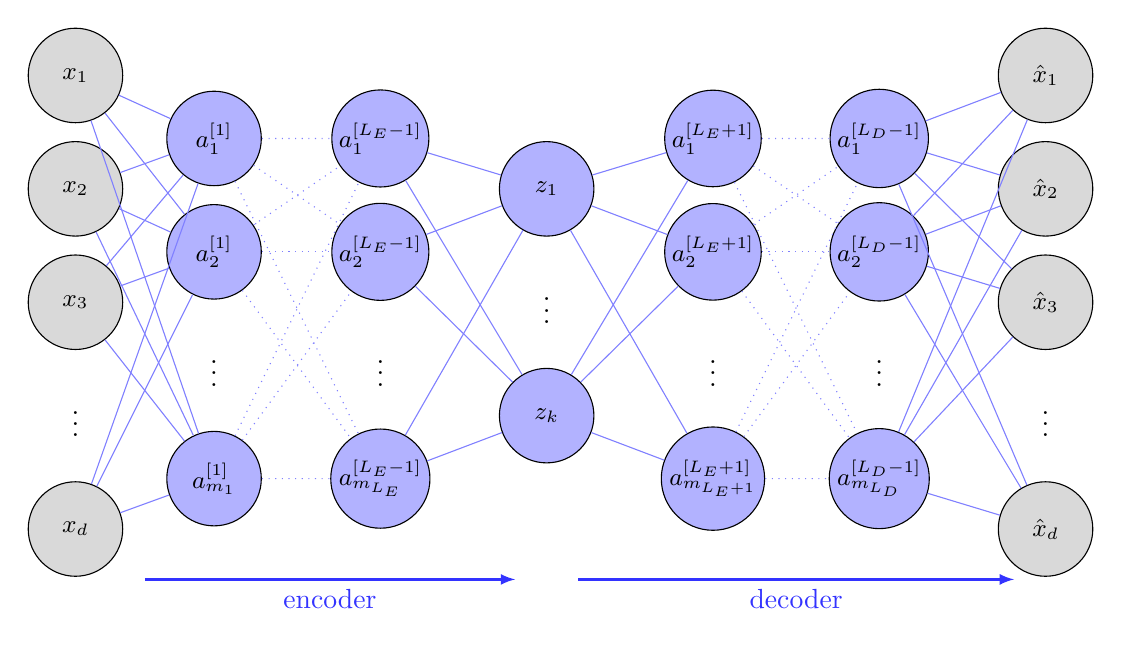
\begin{tikzpicture}[
            scale=0.8,
            node distance=2cm,
            neuron/.style={circle, draw, minimum size=1.2cm, inner sep=1.2pt, font=\small},
            annotation/.style={text width=3cm},
            >=latex
        ]
            % Define some variables for consistent spacing
            \def\layersep{2.2}
            \def\neuronsep{1.8}
            
            % Input layer (x)
            \node[neuron, fill=gray!30] (x1) at (0, 3) {$x_1$};
            \node[neuron, fill=gray!30] (x2) at (0, {3-\neuronsep}) {$x_2$};
            \node[neuron, fill=gray!30] (x3) at (0, {3-2*\neuronsep}) {$x_3$};
            \node at (0, {3-3*\neuronsep}) {$\vdots$};
            \node[neuron, fill=gray!30] (xd) at (0, {3-4*\neuronsep}) {$x_d$};
            
            % First hidden layer (encoder)
            \node[neuron, fill=blue!30] (a11) at (\layersep, 2) {$a^{[1]}_1$};
            \node[neuron, fill=blue!30] (a12) at (\layersep, {2-\neuronsep}) {$a^{[1]}_2$};
            \node at (\layersep, {2-2*\neuronsep}) {$\vdots$};
            \node[neuron, fill=blue!30] (a1m) at (\layersep, {2-3*\neuronsep}) {$a^{[1]}_{m_1}$};
            
            % Last encoder layer
            \node[neuron, fill=blue!30] (aE1) at (2.2*\layersep, 2) {$a^{[L_E-1]}_1$};
            \node[neuron, fill=blue!30] (aE2) at (2.2*\layersep, {2-\neuronsep}) {$a^{[L_E-1]}_2$};
            \node at (2.2*\layersep, {2-2*\neuronsep}) {$\vdots$};
            \node[neuron, fill=blue!30] (aEm) at (2.2*\layersep, {2-3*\neuronsep}) {$a^{[L_E-1]}_{m_{L_E}}$};
            
            % Bottleneck layer (z)
            \node[neuron, fill=blue!30] (z1) at (3.4*\layersep, {1.2-0*\neuronsep}) {$z_1$};
            \node at (3.4*\layersep, {1.2-\neuronsep}) {$\vdots$};
            \node[neuron, fill=blue!30] (zm) at (3.4*\layersep, {1.2-2*\neuronsep}) {$z_k$};
            
            % First decoder layer
            \node[neuron, fill=blue!30] (aD11) at (4.6*\layersep, 2) {$a^{[L_E+1]}_1$};
            \node[neuron, fill=blue!30] (aD12) at (4.6*\layersep, {2-\neuronsep}) {$a^{[L_E+1]}_2$};
            \node at (4.6*\layersep, {2-2*\neuronsep}) {$\vdots$};
            \node[neuron, fill=blue!30] (aD1m) at (4.6*\layersep, {2-3*\neuronsep}) {$a^{[L_E+1]}_{m_{L_E+1}}$};
            
            % Last hidden layer before output
            \node[neuron, fill=blue!30] (aL1) at (5.8*\layersep, 2) {$a^{[L_D-1]}_1$};
            \node[neuron, fill=blue!30] (aL2) at (5.8*\layersep, {2-\neuronsep}) {$a^{[L_D-1]}_2$};
            \node at (5.8*\layersep, {2-2*\neuronsep}) {$\vdots$};
            \node[neuron, fill=blue!30] (aLm) at (5.8*\layersep, {2-3*\neuronsep}) {$a^{[L_D-1]}_{m_{L_D}}$};
            
            % Output layer
            \node[neuron, fill=gray!30] (y1) at (7*\layersep, 3) {$\hat{x}_1$};
            \node[neuron, fill=gray!30] (y2) at (7*\layersep, {3-\neuronsep}) {$\hat{x}_2$};
            \node[neuron, fill=gray!30] (y3) at (7*\layersep, {3-2*\neuronsep}) {$\hat{x}_3$};
            \node at (7*\layersep, {3-3*\neuronsep}) {$\vdots$};
            \node[neuron, fill=gray!30] (yd) at (7*\layersep, {3-4*\neuronsep}) {$\hat{x}_d$};
            
            % Draw connections
            \begin{scope}[blue!50, thin]
              % Input to first hidden
              \foreach \i in {1,2,3,d} {
                  \foreach \j in {1,2,m} {
                      \draw (x\i) -- (a1\j);
                  }
              }
              
              % First hidden to last encoder layer
              \foreach \i in {1,2,m} {
                  \foreach \j in {1,2,m} {
                      \draw[dotted] (a1\i) -- (aE\j);
                  }
              }
              
              % Last encoder to bottleneck
              \foreach \i in {1,2,m} {
                  \foreach \j in {1,m} {
                      \draw (aE\i) -- (z\j);
                  }
              }
              
              % Bottleneck to first decoder
              \foreach \i in {1,m} {
                  \foreach \j in {1,2,m} {
                      \draw (z\i) -- (aD1\j);
                  }
              }
              
              % First decoder to last hidden
              \foreach \i in {1,2,m} {
                  \foreach \j in {1,2,m} {
                      \draw[dotted] (aD1\i) -- (aL\j);
                  }
              }
              
              % Last hidden to output
              \foreach \i in {1,2,m} {
                  \foreach \j in {1,2,3,d} {
                      \draw (aL\i) -- (y\j);
                  }
              }
            \end{scope}
            
            % Add encoder/decoder arrows
            \draw[->, blue!80, thick] (\layersep/2, -5) -- (3.4*\layersep-0.5, -5) 
                node[midway, below, text=blue!80] {encoder};
            \draw[->, blue!80, thick] (3.4*\layersep+0.5, -5) -- (7*\layersep-0.5, -5)
                node[midway, below, text=blue!80] {decoder};
        \end{tikzpicture}
        \caption{A graphical model of an autoencoder. The $z$ is called the \textbf{bottleneck layer}, which compresses the input into a lower-dimensional representation. The $x$ is known as the \textbf{input layer}, the $\hat{x}$ as the \textbf{output layer}, and everything else are \textbf{hidden layers}.} 
        \label{fig:autoencoder}
      \end{figure}
    \end{definition}


    The parameter gradients are obtained by backpropagating the gradient $\nabla_{\theta} \mathcal{L}$ like a regular network, but if we force tied weights (i.e. $W^\ast = W^T$), then $\nabla_{\mathbf{W}} \mathcal{L}$ is the sum of two gradients. This is because $\mathbf{W}$ is present both in the encoder and decoder. 

    I want to train the whole neural network such that the error between $\mathbf{x}$ and $\hat{\mathbf{x}}$ is minimized. We can consider a squared-error, for example. 
    \begin{equation}
      \mathcal{L}(\mathbf{x}, \hat{\mathbf{x}}) = \frac{1}{2} ||\mathbf{x} - \hat{\mathbf{x}}||_2^2
    \end{equation}

    \begin{algo}
      An implementation of an autoencoder in PyTorch is \href{code/autoencoder.html}{here}. 
    \end{algo}

    There are three things we can do to extract meaningful hidden features: 
    \begin{enumerate}
      \item \textbf{Undercomplete Representation}: Make the latent dimension small. It compresses the input, but it may only be good for the training distribution and may not be robust to other types of input. If it is overcomplete, there is no guarantee that we will extract meaningful features. 

      \item \textbf{Denoising Autoencoder}: Injecting noise to the input. The idea is that the representation should be robust to the introduction of noise. We take the original input $\mathbf{x}$ and we randomly assign a subset of the inputs to $0$, with probability $\nu$, similar to dropout, to get our noisy input $\Tilde{\mathbf{x}}$. Then we train the autoencoder with the loss comparing the output $\hat{\mathbf{x}}$ to the original, un-noisy input $\mathbf{x}$. We can do this for Gaussian additive noise too. As the visual below suggests, we are essentially ``pushing" out inputs away from the manifold and training the autoencoder to denoise it, pulling it back. 

        \begin{center}
            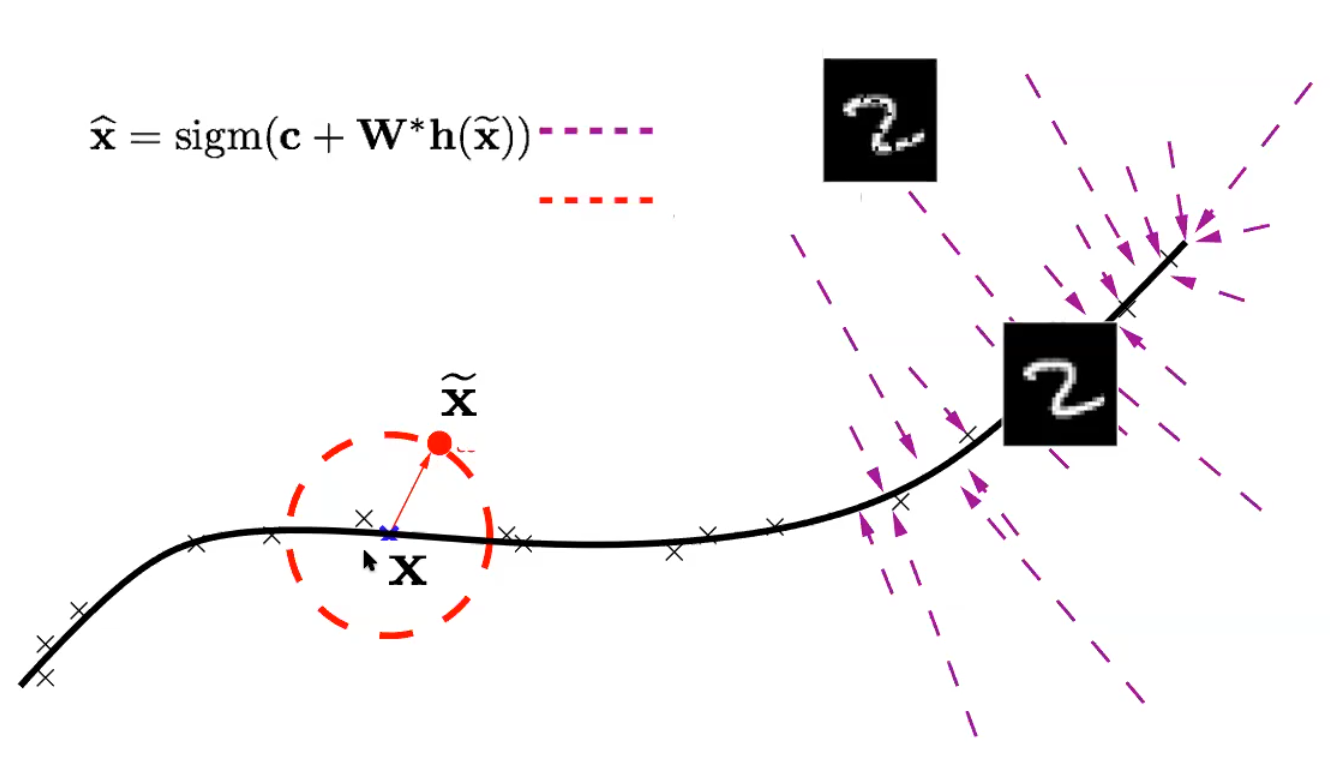
\includegraphics[scale=0.3]{img/denoising_autoencoder.png}
        \end{center}
    
      \item \textbf{Contractive Autoencoder}: If we have the latent dimension greater than the input, then we can just add an explict term in the loss that penalizes that solution (e.g. promoting sparsity). For example, we can have the loss be 
      \[\mathcal{L}(f(\mathbf{x}^{(t)}) + \lambda || \nabla_{\mathbf{x}^{(t)}} \mathbf{h}(\mathbf{x}^{(t)})||^2_F\]
      where 
      \[||\nabla_{\mathbf{x}^{(t)}} \mathbf{h}(\mathbf{x}^{(t)})||_F^2 = \sum_{j, k} \bigg(\frac{\partial h(\mathbf{x}^{(t)})_j}{\partial x_k^{(t)}} \bigg)^2\]
      which forces the encoder to throw away information. If one of the elements are $0$, then we know that the $k$th element of the input has no effect on the $j$th element of the encoded output. Therefore, it tries to throw away as many elements of $\mathbf{x}$ as possible since the identity matrix will have a large Frobenius norm, essentially contracting the input representation.  

      We can also promote sparsity by adding a L1 penalty, forcing the feature space to be sparse. 
    \end{enumerate}

    The \textbf{predictive sparse decomposition} shows that the loss should be 
    \begin{equation}
      \min_{W, W^\ast, \mathbf{z}} ||W^\ast \mathbf{z} - \mathbf{x}||^2_2 + \lambda | \mathbf{z}|_1 + ||\sigma(W \mathbf{x}) - \mathbf{z}||^2_2
    \end{equation}
    where the first term tells the decoder to reconstruct the original input well, the second tells the latent vector to be sparse, and the third tells us that we shouldn't lose too much information when we encode. 

    We could also have \textbf{stacked autoencoders}, with each layer of latent features having some desired sparsity. 

  \subsection{Sequence to Sequence}

    We have mentioned that RNNs and LSTMs have the advantage of mapping from variable length inputs to variable length outputs. This can be done for any length input and any length output. However, the RNN has the problem of \textit{locality}, that the words next to the current word have a greater effect, and we are trying to generate sequences on the fly by reading in each word. Even for bidirectional RNNs, where we go through the whole sentence first, the effects of adjacent words have a greater effect when generating outputs. It would be wiser to read the \textit{whole} sentence and then start to generate a sequence. This is the motivation for the \textbf{encoder-decoder model}. It is conventionally divided into a two-stage network. 
    \begin{enumerate}
      \item The encoder neural net would convert a sequence into a single latent space representation $z = f(x)$. This latent representation $z$ essentially refers to a feature (vector) representation, which is able to capture the underlying semantic information of the input that is useful for predicting the output. 
      \item The decoder neural net would decode this feature vector, called the \textbf{context vector}, into a sequence of the desired output $y = g(z)$ by using it as the initial hidden state. It uses the previous output as the next input for decoding. 
    \end{enumerate}
    Note that the encoder and decoder are two completely separate neural networks with their own parameters. This is important, since the fact that these are two completely separate networks allows us to work in different ``paradigms" within either the feature or target space. For example, if we want to perform machine translation from English to Spanish, our encoder RNN parameters have been tuned to the English syntax and language, while the decoder RNN parameters are tuned to the Spanish language. Since we are modeling different languages, it makes sense to have different sequence models for each one. 

    We will talk about a specific type of encoder-decoder model called \textbf{seq2seq}, which maps sequences to sequences using RNN encoders and decoders. Conventionally, the hidden nodes of the encoder are denoted with $\mathbf{h}$, and those of the decoder are denoted with $\mathbf{s}$. 
    \begin{enumerate}
        \item For the encoder, we take in the inputs $\mathbf{x}_t$ and generate the hidden states as 
        \begin{equation}
          \mathbf{h}_t = f(\mathbf{x}_t, \mathbf{h}_{t-1}) = \mathbf{W}_e \mathbf{h}_{t-1} + \mathbf{U}_e \mathbf{x}_t + \mathbf{b}_e
        \end{equation}
        In general, the encoder transforms the hidden states at all time steps into a context variable through the composition of functions $q$ 
        \[\mathbf{C} = q(\mathbf{h}_1, \mathbf{h}_2, \ldots, \mathbf{h}_T)\]
        In the figure below, the context variable is just $\mathbf{C} = \mathbf{h}_T$. 

        \item Now, given the target output sequence $\hat{\mathbf{y}}_1, \ldots, \hat{\mathbf{y}}_{t^\prime + 1}$ for each timestep $t^\prime$ (we use $t^\prime$ to differentiate from the input sequence time steps), the decoder assigns a predicted probability to each possible token occurring at step $\hat{\mathbf{y}}_{t^\prime + 1}$ conditioned on both the previous tokens $\hat{\mathbf{y}}_1, \ldots, \hat{\mathbf{y}}_{t^\prime + 1}$ and the context variable $\mathbf{C}$, i.e. 
        \[\mathbb{P}(\hat{\mathbf{y}}_{t^\prime + 1} \mid \hat{\mathbf{y}}_1, \ldots, \hat{\mathbf{y}}_{t^\prime + 1}, \mathbf{C})\]
        Therefore, to decode the subsequent token $\hat{\mathbf{y}}_{t^\prime + 1}$, we calculate the hidden state $\mathbf{s}_{t^\prime + 1}$ as a gated hidden unit computed by 
        \[\mathbf{s}_{t^\prime + 1} = g(\mathbf{s}_{t^\prime}, \hat{\mathbf{y}}_{t^\prime}, \mathbf{C})\]
        with the math mentioned \href{https://arxiv.org/pdf/1409.0473.pdf#page=12}{here}. 
    \end{enumerate}

    \begin{figure}[H]
      \centering 
      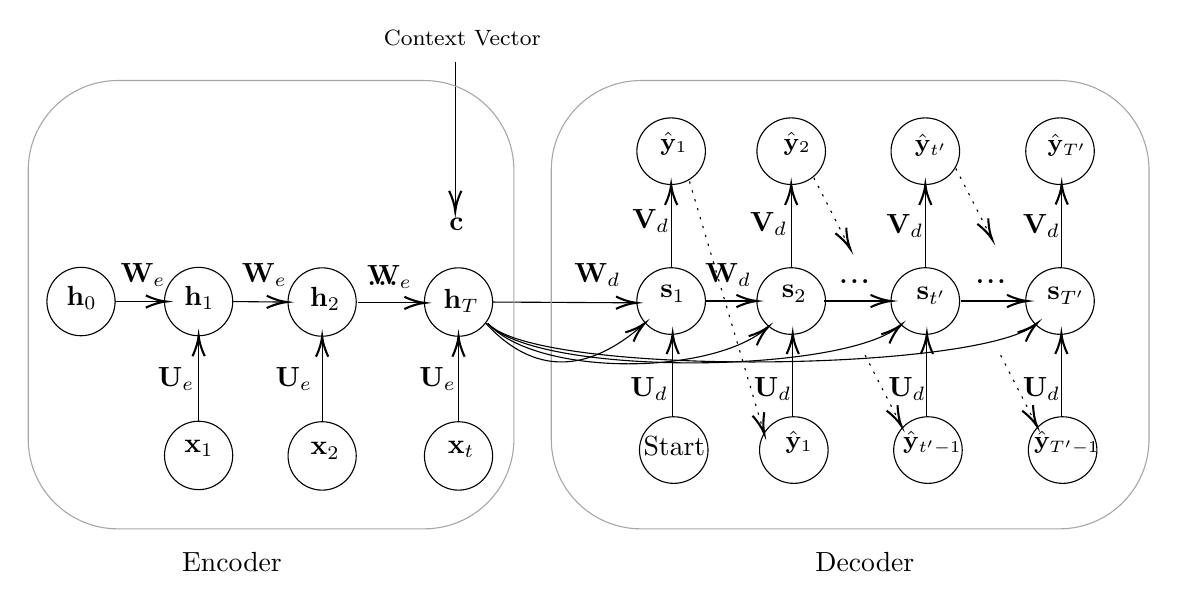
\begin{tikzpicture}[x=0.75pt,y=0.75pt,yscale=-0.9,xscale=0.9]
        %Shape: Ellipse [id:dp12104572681386716] 
        \draw   (169.09,148.58) .. controls (169.09,138.47) and (177.26,130.27) .. (187.34,130.27) .. controls (197.42,130.27) and (205.59,138.47) .. (205.59,148.58) .. controls (205.59,158.69) and (197.42,166.89) .. (187.34,166.89) .. controls (177.26,166.89) and (169.09,158.69) .. (169.09,148.58) -- cycle ;
        %Shape: Ellipse [id:dp741120269708732] 
        \draw   (242.1,148.58) .. controls (242.1,138.47) and (250.27,130.27) .. (260.35,130.27) .. controls (270.43,130.27) and (278.6,138.47) .. (278.6,148.58) .. controls (278.6,158.69) and (270.43,166.89) .. (260.35,166.89) .. controls (250.27,166.89) and (242.1,158.69) .. (242.1,148.58) -- cycle ;
        %Shape: Ellipse [id:dp42031301232731244] 
        \draw   (102.96,148.31) .. controls (102.96,138.2) and (111.14,130) .. (121.22,130) .. controls (131.29,130) and (139.47,138.2) .. (139.47,148.31) .. controls (139.47,158.42) and (131.29,166.62) .. (121.22,166.62) .. controls (111.14,166.62) and (102.96,158.42) .. (102.96,148.31) -- cycle ;
        %Shape: Ellipse [id:dp04610349626863375] 
        \draw   (169.09,230.97) .. controls (169.09,220.86) and (177.26,212.66) .. (187.34,212.66) .. controls (197.42,212.66) and (205.59,220.86) .. (205.59,230.97) .. controls (205.59,241.08) and (197.42,249.28) .. (187.34,249.28) .. controls (177.26,249.28) and (169.09,241.08) .. (169.09,230.97) -- cycle ;
        %Shape: Ellipse [id:dp7588227428266139] 
        \draw   (242.1,230.97) .. controls (242.1,220.86) and (250.27,212.66) .. (260.35,212.66) .. controls (270.43,212.66) and (278.6,220.86) .. (278.6,230.97) .. controls (278.6,241.08) and (270.43,249.28) .. (260.35,249.28) .. controls (250.27,249.28) and (242.1,241.08) .. (242.1,230.97) -- cycle ;
        %Shape: Ellipse [id:dp3672959591373348] 
        \draw   (102.96,230.7) .. controls (102.96,220.59) and (111.14,212.39) .. (121.22,212.39) .. controls (131.29,212.39) and (139.47,220.59) .. (139.47,230.7) .. controls (139.47,240.81) and (131.29,249.01) .. (121.22,249.01) .. controls (111.14,249.01) and (102.96,240.81) .. (102.96,230.7) -- cycle ;
        %Straight Lines [id:da21018477228753185] 
        \draw [color={rgb, 255:red, 0; green, 0; blue, 0 }  ,draw opacity=1 ]   (121.22,212.39) -- (121.22,168.62) ;
        \draw [shift={(121.22,166.62)}, rotate = 90] [color={rgb, 255:red, 0; green, 0; blue, 0 }  ,draw opacity=1 ][line width=0.75]    (10.93,-3.29) .. controls (6.95,-1.4) and (3.31,-0.3) .. (0,0) .. controls (3.31,0.3) and (6.95,1.4) .. (10.93,3.29)   ;
        %Straight Lines [id:da17363282179045836] 
        \draw [color={rgb, 255:red, 0; green, 0; blue, 0 }  ,draw opacity=1 ]   (187.34,212.66) -- (187.34,168.89) ;
        \draw [shift={(187.34,166.89)}, rotate = 90] [color={rgb, 255:red, 0; green, 0; blue, 0 }  ,draw opacity=1 ][line width=0.75]    (10.93,-3.29) .. controls (6.95,-1.4) and (3.31,-0.3) .. (0,0) .. controls (3.31,0.3) and (6.95,1.4) .. (10.93,3.29)   ;
        %Straight Lines [id:da40218372998636487] 
        \draw [color={rgb, 255:red, 0; green, 0; blue, 0 }  ,draw opacity=1 ]   (260.35,212.66) -- (260.35,168.89) ;
        \draw [shift={(260.35,166.89)}, rotate = 90] [color={rgb, 255:red, 0; green, 0; blue, 0 }  ,draw opacity=1 ][line width=0.75]    (10.93,-3.29) .. controls (6.95,-1.4) and (3.31,-0.3) .. (0,0) .. controls (3.31,0.3) and (6.95,1.4) .. (10.93,3.29)   ;
        %Shape: Ellipse [id:dp9751332219640756] 
        \draw   (40,148.31) .. controls (40,138.2) and (48.17,130) .. (58.25,130) .. controls (68.33,130) and (76.5,138.2) .. (76.5,148.31) .. controls (76.5,158.42) and (68.33,166.62) .. (58.25,166.62) .. controls (48.17,166.62) and (40,158.42) .. (40,148.31) -- cycle ;
        %Straight Lines [id:da988218839650463] 
        \draw [color={rgb, 255:red, 0; green, 0; blue, 0 }  ,draw opacity=1 ]   (76.5,148.31) -- (101.88,148.31) ;
        \draw [shift={(103.88,148.31)}, rotate = 180] [color={rgb, 255:red, 0; green, 0; blue, 0 }  ,draw opacity=1 ][line width=0.75]    (10.93,-3.29) .. controls (6.95,-1.4) and (3.31,-0.3) .. (0,0) .. controls (3.31,0.3) and (6.95,1.4) .. (10.93,3.29)   ;
        %Straight Lines [id:da8149363438054458] 
        \draw [color={rgb, 255:red, 0; green, 0; blue, 0 }  ,draw opacity=1 ]   (139.47,148.31) -- (166.6,148.59) ;
        \draw [shift={(168.6,148.61)}, rotate = 180.59] [color={rgb, 255:red, 0; green, 0; blue, 0 }  ,draw opacity=1 ][line width=0.75]    (10.93,-3.29) .. controls (6.95,-1.4) and (3.31,-0.3) .. (0,0) .. controls (3.31,0.3) and (6.95,1.4) .. (10.93,3.29)   ;
        %Shape: Ellipse [id:dp8769921800297902] 
        \draw   (420.09,67.83) .. controls (420.09,57.98) and (428.31,50) .. (438.44,50) .. controls (448.58,50) and (456.79,57.98) .. (456.79,67.83) .. controls (456.79,77.67) and (448.58,85.65) .. (438.44,85.65) .. controls (428.31,85.65) and (420.09,77.67) .. (420.09,67.83) -- cycle ;
        %Shape: Ellipse [id:dp8525299588463036] 
        \draw   (491.9,67.83) .. controls (491.9,57.98) and (500.11,50) .. (510.25,50) .. controls (520.38,50) and (528.6,57.98) .. (528.6,67.83) .. controls (528.6,77.67) and (520.38,85.65) .. (510.25,85.65) .. controls (500.11,85.65) and (491.9,77.67) .. (491.9,67.83) -- cycle ;
        %Shape: Ellipse [id:dp09036435821311728] 
        \draw   (420.09,148.04) .. controls (420.09,138.2) and (428.31,130.21) .. (438.44,130.21) .. controls (448.58,130.21) and (456.79,138.2) .. (456.79,148.04) .. controls (456.79,157.88) and (448.58,165.87) .. (438.44,165.87) .. controls (428.31,165.87) and (420.09,157.88) .. (420.09,148.04) -- cycle ;
        %Shape: Ellipse [id:dp23880588274822712] 
        \draw   (491.9,148.04) .. controls (491.9,138.2) and (500.11,130.21) .. (510.25,130.21) .. controls (520.38,130.21) and (528.6,138.2) .. (528.6,148.04) .. controls (528.6,157.88) and (520.38,165.87) .. (510.25,165.87) .. controls (500.11,165.87) and (491.9,157.88) .. (491.9,148.04) -- cycle ;
        %Shape: Ellipse [id:dp4615954589889102] 
        \draw   (355.82,148.04) .. controls (355.82,138.2) and (364.04,130.21) .. (374.17,130.21) .. controls (384.3,130.21) and (392.52,138.2) .. (392.52,148.04) .. controls (392.52,157.88) and (384.3,165.87) .. (374.17,165.87) .. controls (364.04,165.87) and (355.82,157.88) .. (355.82,148.04) -- cycle ;
        %Straight Lines [id:da8663141237622789] 
        \draw [color={rgb, 255:red, 0; green, 0; blue, 0 }  ,draw opacity=1 ]   (392.52,148.04) -- (418.05,148.04) ;
        \draw [shift={(420.05,148.04)}, rotate = 180] [color={rgb, 255:red, 0; green, 0; blue, 0 }  ,draw opacity=1 ][line width=0.75]    (10.93,-3.29) .. controls (6.95,-1.4) and (3.31,-0.3) .. (0,0) .. controls (3.31,0.3) and (6.95,1.4) .. (10.93,3.29)   ;
        %Straight Lines [id:da054789319283937044] 
        \draw [color={rgb, 255:red, 0; green, 0; blue, 0 }  ,draw opacity=1 ]   (456.2,148.04) -- (489.9,148.04) ;
        \draw [shift={(491.9,148.04)}, rotate = 180] [color={rgb, 255:red, 0; green, 0; blue, 0 }  ,draw opacity=1 ][line width=0.75]    (10.93,-3.29) .. controls (6.95,-1.4) and (3.31,-0.3) .. (0,0) .. controls (3.31,0.3) and (6.95,1.4) .. (10.93,3.29)   ;
        %Straight Lines [id:da8426206211081082] 
        \draw [color={rgb, 255:red, 0; green, 0; blue, 0 }  ,draw opacity=1 ]   (438.44,130.21) -- (438.44,87.65) ;
        \draw [shift={(438.44,85.65)}, rotate = 90] [color={rgb, 255:red, 0; green, 0; blue, 0 }  ,draw opacity=1 ][line width=0.75]    (10.93,-3.29) .. controls (6.95,-1.4) and (3.31,-0.3) .. (0,0) .. controls (3.31,0.3) and (6.95,1.4) .. (10.93,3.29)   ;
        %Straight Lines [id:da11805221789762355] 
        \draw [color={rgb, 255:red, 0; green, 0; blue, 0 }  ,draw opacity=1 ]   (510.25,130.21) -- (510.25,99.91) -- (510.25,87.65) ;
        \draw [shift={(510.25,85.65)}, rotate = 90] [color={rgb, 255:red, 0; green, 0; blue, 0 }  ,draw opacity=1 ][line width=0.75]    (10.93,-3.29) .. controls (6.95,-1.4) and (3.31,-0.3) .. (0,0) .. controls (3.31,0.3) and (6.95,1.4) .. (10.93,3.29)   ;
        %Shape: Ellipse [id:dp22353660348109727] 
        \draw   (355.82,67.83) .. controls (355.82,57.98) and (364.04,50) .. (374.17,50) .. controls (384.3,50) and (392.52,57.98) .. (392.52,67.83) .. controls (392.52,77.67) and (384.3,85.65) .. (374.17,85.65) .. controls (364.04,85.65) and (355.82,77.67) .. (355.82,67.83) -- cycle ;
        %Straight Lines [id:da15189468948594165] 
        \draw [color={rgb, 255:red, 0; green, 0; blue, 0 }  ,draw opacity=1 ]   (374.17,130.21) -- (374.17,99.91) -- (374.17,87.65) ;
        \draw [shift={(374.17,85.65)}, rotate = 90] [color={rgb, 255:red, 0; green, 0; blue, 0 }  ,draw opacity=1 ][line width=0.75]    (10.93,-3.29) .. controls (6.95,-1.4) and (3.31,-0.3) .. (0,0) .. controls (3.31,0.3) and (6.95,1.4) .. (10.93,3.29)   ;
        %Straight Lines [id:da7646592734808089] 
        \draw [color={rgb, 255:red, 0; green, 0; blue, 0 }  ,draw opacity=1 ]   (206.6,149.04) -- (240.3,149.04) ;
        \draw [shift={(242.3,149.04)}, rotate = 180] [color={rgb, 255:red, 0; green, 0; blue, 0 }  ,draw opacity=1 ][line width=0.75]    (10.93,-3.29) .. controls (6.95,-1.4) and (3.31,-0.3) .. (0,0) .. controls (3.31,0.3) and (6.95,1.4) .. (10.93,3.29)   ;
        %Straight Lines [id:da7609105327490961] 
        \draw    (258.6,20) -- (258.6,98) ;
        \draw [shift={(258.6,100)}, rotate = 270] [color={rgb, 255:red, 0; green, 0; blue, 0 }  ][line width=0.75]    (10.93,-3.29) .. controls (6.95,-1.4) and (3.31,-0.3) .. (0,0) .. controls (3.31,0.3) and (6.95,1.4) .. (10.93,3.29)   ;
        %Straight Lines [id:da815869668900407] 
        \draw [color={rgb, 255:red, 0; green, 0; blue, 0 }  ,draw opacity=1 ]   (278.6,148.58) -- (353.6,148.99) ;
        \draw [shift={(355.6,149)}, rotate = 180.31] [color={rgb, 255:red, 0; green, 0; blue, 0 }  ,draw opacity=1 ][line width=0.75]    (10.93,-3.29) .. controls (6.95,-1.4) and (3.31,-0.3) .. (0,0) .. controls (3.31,0.3) and (6.95,1.4) .. (10.93,3.29)   ;
        %Rounded Rect [id:dp8974917713272867] 
        \draw  [color={rgb, 255:red, 167; green, 167; blue, 167 }  ,draw opacity=1 ] (30,78) .. controls (30,51.49) and (51.49,30) .. (78,30) -- (242,30) .. controls (268.51,30) and (290,51.49) .. (290,78) -- (290,222) .. controls (290,248.51) and (268.51,270) .. (242,270) -- (78,270) .. controls (51.49,270) and (30,248.51) .. (30,222) -- cycle ;
        %Rounded Rect [id:dp621652359446494] 
        \draw  [color={rgb, 255:red, 167; green, 167; blue, 167 }  ,draw opacity=1 ] (310,78) .. controls (310,51.49) and (331.49,30) .. (358,30) -- (582,30) .. controls (608.51,30) and (630,51.49) .. (630,78) -- (630,222) .. controls (630,248.51) and (608.51,270) .. (582,270) -- (358,270) .. controls (331.49,270) and (310,248.51) .. (310,222) -- cycle ;
        %Straight Lines [id:da2968728075840934] 
        \draw [color={rgb, 255:red, 0; green, 0; blue, 0 }  ,draw opacity=1 ]   (439.27,210) -- (439.27,167.44) ;
        \draw [shift={(439.27,165.44)}, rotate = 90] [color={rgb, 255:red, 0; green, 0; blue, 0 }  ,draw opacity=1 ][line width=0.75]    (10.93,-3.29) .. controls (6.95,-1.4) and (3.31,-0.3) .. (0,0) .. controls (3.31,0.3) and (6.95,1.4) .. (10.93,3.29)   ;
        %Straight Lines [id:da38515939024710244] 
        \draw [color={rgb, 255:red, 0; green, 0; blue, 0 }  ,draw opacity=1 ]   (511.08,210) -- (511.08,179.7) -- (511.08,167.44) ;
        \draw [shift={(511.08,165.44)}, rotate = 90] [color={rgb, 255:red, 0; green, 0; blue, 0 }  ,draw opacity=1 ][line width=0.75]    (10.93,-3.29) .. controls (6.95,-1.4) and (3.31,-0.3) .. (0,0) .. controls (3.31,0.3) and (6.95,1.4) .. (10.93,3.29)   ;
        %Straight Lines [id:da14741802814240956] 
        \draw [color={rgb, 255:red, 0; green, 0; blue, 0 }  ,draw opacity=1 ]   (375,210) -- (375,193.6) -- (375,179.7) -- (375,167.44) ;
        \draw [shift={(375,165.44)}, rotate = 90] [color={rgb, 255:red, 0; green, 0; blue, 0 }  ,draw opacity=1 ][line width=0.75]    (10.93,-3.29) .. controls (6.95,-1.4) and (3.31,-0.3) .. (0,0) .. controls (3.31,0.3) and (6.95,1.4) .. (10.93,3.29)   ;
        %Shape: Ellipse [id:dp7615118627097319] 
        \draw   (421.5,227.83) .. controls (421.5,217.98) and (429.71,210) .. (439.85,210) .. controls (449.98,210) and (458.2,217.98) .. (458.2,227.83) .. controls (458.2,237.67) and (449.98,245.65) .. (439.85,245.65) .. controls (429.71,245.65) and (421.5,237.67) .. (421.5,227.83) -- cycle ;
        %Shape: Ellipse [id:dp640367209409753] 
        \draw   (493.3,227.83) .. controls (493.3,217.98) and (501.52,210) .. (511.65,210) .. controls (521.78,210) and (530,217.98) .. (530,227.83) .. controls (530,237.67) and (521.78,245.65) .. (511.65,245.65) .. controls (501.52,245.65) and (493.3,237.67) .. (493.3,227.83) -- cycle ;
        %Shape: Ellipse [id:dp18357530976130754] 
        \draw   (357.22,227.83) .. controls (357.22,217.98) and (365.44,210) .. (375.57,210) .. controls (385.71,210) and (393.92,217.98) .. (393.92,227.83) .. controls (393.92,237.67) and (385.71,245.65) .. (375.57,245.65) .. controls (365.44,245.65) and (357.22,237.67) .. (357.22,227.83) -- cycle ;
        %Straight Lines [id:da039581984918104274] 
        \draw  [dash pattern={on 0.84pt off 2.51pt}]  (384,84) -- (423.43,217.08) ;
        \draw [shift={(424,219)}, rotate = 253.5] [color={rgb, 255:red, 0; green, 0; blue, 0 }  ][line width=0.75]    (10.93,-3.29) .. controls (6.95,-1.4) and (3.31,-0.3) .. (0,0) .. controls (3.31,0.3) and (6.95,1.4) .. (10.93,3.29)   ;
        %Straight Lines [id:da6000754918163929] 
        \draw  [dash pattern={on 0.84pt off 2.51pt}]  (450.55,82.04) -- (469.09,118.22) ;
        \draw [shift={(470,120)}, rotate = 242.87] [color={rgb, 255:red, 0; green, 0; blue, 0 }  ][line width=0.75]    (10.93,-3.29) .. controls (6.95,-1.4) and (3.31,-0.3) .. (0,0) .. controls (3.31,0.3) and (6.95,1.4) .. (10.93,3.29)   ;
        %Straight Lines [id:da5632246037194519] 
        \draw [color={rgb, 255:red, 0; green, 0; blue, 0 }  ,draw opacity=1 ]   (529.2,148.04) -- (562.9,148.04) ;
        \draw [shift={(564.9,148.04)}, rotate = 180] [color={rgb, 255:red, 0; green, 0; blue, 0 }  ,draw opacity=1 ][line width=0.75]    (10.93,-3.29) .. controls (6.95,-1.4) and (3.31,-0.3) .. (0,0) .. controls (3.31,0.3) and (6.95,1.4) .. (10.93,3.29)   ;
        %Straight Lines [id:da564576595545853] 
        \draw  [dash pattern={on 0.84pt off 2.51pt}]  (478,177) -- (496.54,213.18) ;
        \draw [shift={(497.45,214.96)}, rotate = 242.87] [color={rgb, 255:red, 0; green, 0; blue, 0 }  ][line width=0.75]    (10.93,-3.29) .. controls (6.95,-1.4) and (3.31,-0.3) .. (0,0) .. controls (3.31,0.3) and (6.95,1.4) .. (10.93,3.29)   ;
        %Straight Lines [id:da2885206646010938] 
        \draw  [dash pattern={on 0.84pt off 2.51pt}]  (526.55,77.04) -- (545.09,113.22) ;
        \draw [shift={(546,115)}, rotate = 242.87] [color={rgb, 255:red, 0; green, 0; blue, 0 }  ][line width=0.75]    (10.93,-3.29) .. controls (6.95,-1.4) and (3.31,-0.3) .. (0,0) .. controls (3.31,0.3) and (6.95,1.4) .. (10.93,3.29)   ;
        %Curve Lines [id:da21184366007833177] 
        \draw    (275,160) .. controls (301.1,188.26) and (329.62,186.42) .. (358.67,161.17) ;
        \draw [shift={(360,160)}, rotate = 138.23] [color={rgb, 255:red, 0; green, 0; blue, 0 }  ][line width=0.75]    (10.93,-3.29) .. controls (6.95,-1.4) and (3.31,-0.3) .. (0,0) .. controls (3.31,0.3) and (6.95,1.4) .. (10.93,3.29)   ;
        %Curve Lines [id:da7156893211463737] 
        \draw    (276,160) .. controls (302.1,188.26) and (393.69,188.36) .. (424.63,163.17) ;
        \draw [shift={(426,162)}, rotate = 138.23] [color={rgb, 255:red, 0; green, 0; blue, 0 }  ][line width=0.75]    (10.93,-3.29) .. controls (6.95,-1.4) and (3.31,-0.3) .. (0,0) .. controls (3.31,0.3) and (6.95,1.4) .. (10.93,3.29)   ;
        %Curve Lines [id:da8926144138863956] 
        \draw    (276,160) .. controls (302.1,188.26) and (462.57,187.39) .. (495.58,162.17) ;
        \draw [shift={(497,161)}, rotate = 138.23] [color={rgb, 255:red, 0; green, 0; blue, 0 }  ][line width=0.75]    (10.93,-3.29) .. controls (6.95,-1.4) and (3.31,-0.3) .. (0,0) .. controls (3.31,0.3) and (6.95,1.4) .. (10.93,3.29)   ;
        %Shape: Ellipse [id:dp13692419886270235] 
        \draw   (564,67.83) .. controls (564,57.98) and (572.22,50) .. (582.35,50) .. controls (592.48,50) and (600.7,57.98) .. (600.7,67.83) .. controls (600.7,77.67) and (592.48,85.65) .. (582.35,85.65) .. controls (572.22,85.65) and (564,77.67) .. (564,67.83) -- cycle ;
        %Shape: Ellipse [id:dp3366510546944117] 
        \draw   (564,148.04) .. controls (564,138.2) and (572.22,130.21) .. (582.35,130.21) .. controls (592.48,130.21) and (600.7,138.2) .. (600.7,148.04) .. controls (600.7,157.88) and (592.48,165.87) .. (582.35,165.87) .. controls (572.22,165.87) and (564,157.88) .. (564,148.04) -- cycle ;
        %Shape: Ellipse [id:dp8287297044956745] 
        \draw   (565.4,227.83) .. controls (565.4,217.98) and (573.62,210) .. (583.75,210) .. controls (593.89,210) and (602.1,217.98) .. (602.1,227.83) .. controls (602.1,237.67) and (593.89,245.65) .. (583.75,245.65) .. controls (573.62,245.65) and (565.4,237.67) .. (565.4,227.83) -- cycle ;
        %Straight Lines [id:da11725970020422505] 
        \draw [color={rgb, 255:red, 0; green, 0; blue, 0 }  ,draw opacity=1 ]   (583.25,130) -- (583.25,99.7) -- (583.25,87.44) ;
        \draw [shift={(583.25,85.44)}, rotate = 90] [color={rgb, 255:red, 0; green, 0; blue, 0 }  ,draw opacity=1 ][line width=0.75]    (10.93,-3.29) .. controls (6.95,-1.4) and (3.31,-0.3) .. (0,0) .. controls (3.31,0.3) and (6.95,1.4) .. (10.93,3.29)   ;
        %Straight Lines [id:da9847989868461862] 
        \draw [color={rgb, 255:red, 0; green, 0; blue, 0 }  ,draw opacity=1 ]   (583.08,210) -- (583.08,179.7) -- (583.08,167.44) ;
        \draw [shift={(583.08,165.44)}, rotate = 90] [color={rgb, 255:red, 0; green, 0; blue, 0 }  ,draw opacity=1 ][line width=0.75]    (10.93,-3.29) .. controls (6.95,-1.4) and (3.31,-0.3) .. (0,0) .. controls (3.31,0.3) and (6.95,1.4) .. (10.93,3.29)   ;
        %Curve Lines [id:da42556894346201957] 
        \draw    (276,160) .. controls (302.1,188.26) and (533.4,186.42) .. (568.53,161.17) ;
        \draw [shift={(570,160)}, rotate = 138.23] [color={rgb, 255:red, 0; green, 0; blue, 0 }  ][line width=0.75]    (10.93,-3.29) .. controls (6.95,-1.4) and (3.31,-0.3) .. (0,0) .. controls (3.31,0.3) and (6.95,1.4) .. (10.93,3.29)   ;
        %Straight Lines [id:da7291299431653597] 
        \draw  [dash pattern={on 0.84pt off 2.51pt}]  (550.55,177.04) -- (569.09,213.22) ;
        \draw [shift={(570,215)}, rotate = 242.87] [color={rgb, 255:red, 0; green, 0; blue, 0 }  ][line width=0.75]    (10.93,-3.29) .. controls (6.95,-1.4) and (3.31,-0.3) .. (0,0) .. controls (3.31,0.3) and (6.95,1.4) .. (10.93,3.29)   ;

        % Text Node
        \draw (112.17,138.79) node [anchor=north west][inner sep=0.75pt]  [font=\normalsize]  {$\mathbf{h}_{1}$};
        % Text Node
        \draw (179.49,139.39) node [anchor=north west][inner sep=0.75pt]  [font=\normalsize]  {$\mathbf{h}_{2}$};
        % Text Node
        \draw (251,140.4) node [anchor=north west][inner sep=0.75pt]  [font=\normalsize]  {$\mathbf{h}_{T}$};
        % Text Node
        \draw (112.22,221.19) node [anchor=north west][inner sep=0.75pt]  [font=\normalsize]  {$\mathbf{x}_{1}$};
        % Text Node
        \draw (179.71,222.45) node [anchor=north west][inner sep=0.75pt]  [font=\normalsize]  {$\mathbf{x}_{2}$};
        % Text Node
        \draw (253.26,221.45) node [anchor=north west][inner sep=0.75pt]  [font=\normalsize]  {$\mathbf{x}_{t}$};
        % Text Node
        \draw (49.21,138.79) node [anchor=north west][inner sep=0.75pt]  [font=\normalsize]  {$\mathbf{h}_{0}$};
        % Text Node
        \draw (433,56.4) node [anchor=north west][inner sep=0.75pt]  [font=\small]  {$\hat{\mathbf{y}}_{2}$};
        % Text Node
        \draw (367,138.4) node [anchor=north west][inner sep=0.75pt]  [font=\normalsize]  {$\mathbf{s}_{1}$};
        % Text Node
        \draw (504.12,139.44) node [anchor=north west][inner sep=0.75pt]  [font=\normalsize]  {$\mathbf{s}_{t^{\prime }}$};
        % Text Node
        \draw (503.2,57.4) node [anchor=north west][inner sep=0.75pt]  [font=\small]  {$\hat{\mathbf{y}}_{t^{\prime }}$};
        % Text Node
        \draw (367,56.4) node [anchor=north west][inner sep=0.75pt]  [font=\small]  {$\hat{\mathbf{y}}_{1}$};
        % Text Node
        \draw (462.2,135) node [anchor=north west][inner sep=0.75pt]  [font=\Large] [align=left] {...};
        % Text Node
        \draw (209.6,136) node [anchor=north west][inner sep=0.75pt]  [font=\Large] [align=left] {...};
        % Text Node
        \draw (219,2) node [anchor=north west][inner sep=0.75pt]   [align=left] {{\footnotesize Context Vector}};
        % Text Node
        \draw (111,281) node [anchor=north west][inner sep=0.75pt]   [align=left] {Encoder};
        % Text Node
        \draw (450,281) node [anchor=north west][inner sep=0.75pt]   [align=left] {Decoder};
        % Text Node
        \draw (78,126.4) node [anchor=north west][inner sep=0.75pt]  [font=\normalsize,color={rgb, 255:red, 0; green, 0; blue, 0 }  ,opacity=1 ]  {$\mathbf{W}_{e}$};
        % Text Node
        \draw (98,182.4) node [anchor=north west][inner sep=0.75pt]  [font=\normalsize,color={rgb, 255:red, 0; green, 0; blue, 0 }  ,opacity=1 ]  {$\mathbf{U}_{e}$};
        % Text Node
        \draw (352,97.4) node [anchor=north west][inner sep=0.75pt]  [font=\normalsize,color={rgb, 255:red, 0; green, 0; blue, 0 }  ,opacity=1 ]  {$\mathbf{V}_{d}$};
        % Text Node
        \draw (321,126.4) node [anchor=north west][inner sep=0.75pt]  [font=\normalsize,color={rgb, 255:red, 0; green, 0; blue, 0 }  ,opacity=1 ]  {$\mathbf{W}_{d}$};
        % Text Node
        \draw (161,182.4) node [anchor=north west][inner sep=0.75pt]  [font=\normalsize,color={rgb, 255:red, 0; green, 0; blue, 0 }  ,opacity=1 ]  {$\mathbf{U}_{e}$};
        % Text Node
        \draw (238,182.4) node [anchor=north west][inner sep=0.75pt]  [font=\normalsize,color={rgb, 255:red, 0; green, 0; blue, 0 }  ,opacity=1 ]  {$\mathbf{U}_{e}$};
        % Text Node
        \draw (143,126.4) node [anchor=north west][inner sep=0.75pt]  [font=\normalsize,color={rgb, 255:red, 0; green, 0; blue, 0 }  ,opacity=1 ]  {$\mathbf{W}_{e}$};
        % Text Node
        \draw (210,127.4) node [anchor=north west][inner sep=0.75pt]  [font=\normalsize,color={rgb, 255:red, 0; green, 0; blue, 0 }  ,opacity=1 ]  {$\mathbf{W}_{e}$};
        % Text Node
        \draw (415,99.4) node [anchor=north west][inner sep=0.75pt]  [font=\normalsize,color={rgb, 255:red, 0; green, 0; blue, 0 }  ,opacity=1 ]  {$\mathbf{V}_{d}$};
        % Text Node
        \draw (488,100.4) node [anchor=north west][inner sep=0.75pt]  [font=\normalsize,color={rgb, 255:red, 0; green, 0; blue, 0 }  ,opacity=1 ]  {$\mathbf{V}_{d}$};
        % Text Node
        \draw (391,126.4) node [anchor=north west][inner sep=0.75pt]  [font=\normalsize,color={rgb, 255:red, 0; green, 0; blue, 0 }  ,opacity=1 ]  {$\mathbf{W}_{d}$};
        % Text Node
        \draw (497,216.4) node [anchor=north west][inner sep=0.75pt]  [font=\small]  {$\hat{\mathbf{y}}_{t^{\prime } -1}$};
        % Text Node
        \draw (434,216.4) node [anchor=north west][inner sep=0.75pt]  [font=\small]  {$\hat{\mathbf{y}}_{1}$};
        % Text Node
        \draw (358,219) node [anchor=north west][inner sep=0.75pt]   [align=left] {Start};
        % Text Node
        \draw (351,187.4) node [anchor=north west][inner sep=0.75pt]  [font=\normalsize,color={rgb, 255:red, 0; green, 0; blue, 0 }  ,opacity=1 ]  {$\mathbf{U}_{d}$};
        % Text Node
        \draw (417,187.4) node [anchor=north west][inner sep=0.75pt]  [font=\normalsize,color={rgb, 255:red, 0; green, 0; blue, 0 }  ,opacity=1 ]  {$\mathbf{U}_{d}$};
        % Text Node
        \draw (489,187.4) node [anchor=north west][inner sep=0.75pt]  [font=\normalsize,color={rgb, 255:red, 0; green, 0; blue, 0 }  ,opacity=1 ]  {$\mathbf{U}_{d}$};
        % Text Node
        \draw (432,138.4) node [anchor=north west][inner sep=0.75pt]  [font=\normalsize]  {$\mathbf{s}_{2}$};
        % Text Node
        \draw (535.2,135) node [anchor=north west][inner sep=0.75pt]  [font=\Large] [align=left] {...};
        % Text Node
        \draw (574.23,139.44) node [anchor=north west][inner sep=0.75pt]  [font=\normalsize]  {$\mathbf{s}_{T^{\prime }}$};
        % Text Node
        \draw (574.3,57.4) node [anchor=north west][inner sep=0.75pt]  [font=\small]  {$\hat{\mathbf{y}}_{T^{\prime }}$};
        % Text Node
        \draw (567.1,216.4) node [anchor=north west][inner sep=0.75pt]  [font=\small]  {$\hat{\mathbf{y}}_{T^{\prime } -1}$};
        % Text Node
        \draw (561,100.19) node [anchor=north west][inner sep=0.75pt]  [font=\normalsize,color={rgb, 255:red, 0; green, 0; blue, 0 }  ,opacity=1 ]  {$\mathbf{V}_{d}$};
        % Text Node
        \draw (561,187.4) node [anchor=north west][inner sep=0.75pt]  [font=\normalsize,color={rgb, 255:red, 0; green, 0; blue, 0 }  ,opacity=1 ]  {$\mathbf{U}_{d}$};
        % Text Node
        \draw (254,102.4) node [anchor=north west][inner sep=0.75pt]  [font=\normalsize]  {$\mathbf{c}$};
      \end{tikzpicture}
      \caption{} 
      \label{fig:encoder_decoder_rnn}
    \end{figure}

    Again, note that this encoder-decoder model is comprised of two completely separate deep models with their own parameters, and so it is \textit{not} simply just one long RNN that starts generating outputs only after it takes in all the inputs. Sometimes, the inputs to the decoder may not be shown in diagrams since it is assumed that they are always the previous node's outputs. Furthermore, we can also see that there is no clear-defined first input for the decoder model, since this is the beginning of the sequence. We usually just put some special ``start" element in here to denote the beginning of the output. 

    Here is a diagram for a encoder-decoder model for a 2-layer LSTM which is the standard for practical use, which encodes the sentence meaning in the vectors $\mathbf{c}_t^{[2]}, \mathbf{h}_t ^{[2]}, \mathbf{c}_t^{[1]}, \mathbf{h}_t^{[1]}$. In practice, high performing RNNs are usually multilayer (almost alway greater than 1, but diminishing performance returns as number of layers increases), but are not as deep as convolutional or feed forward networks. 

    \begin{figure}[H]
      \centering 
      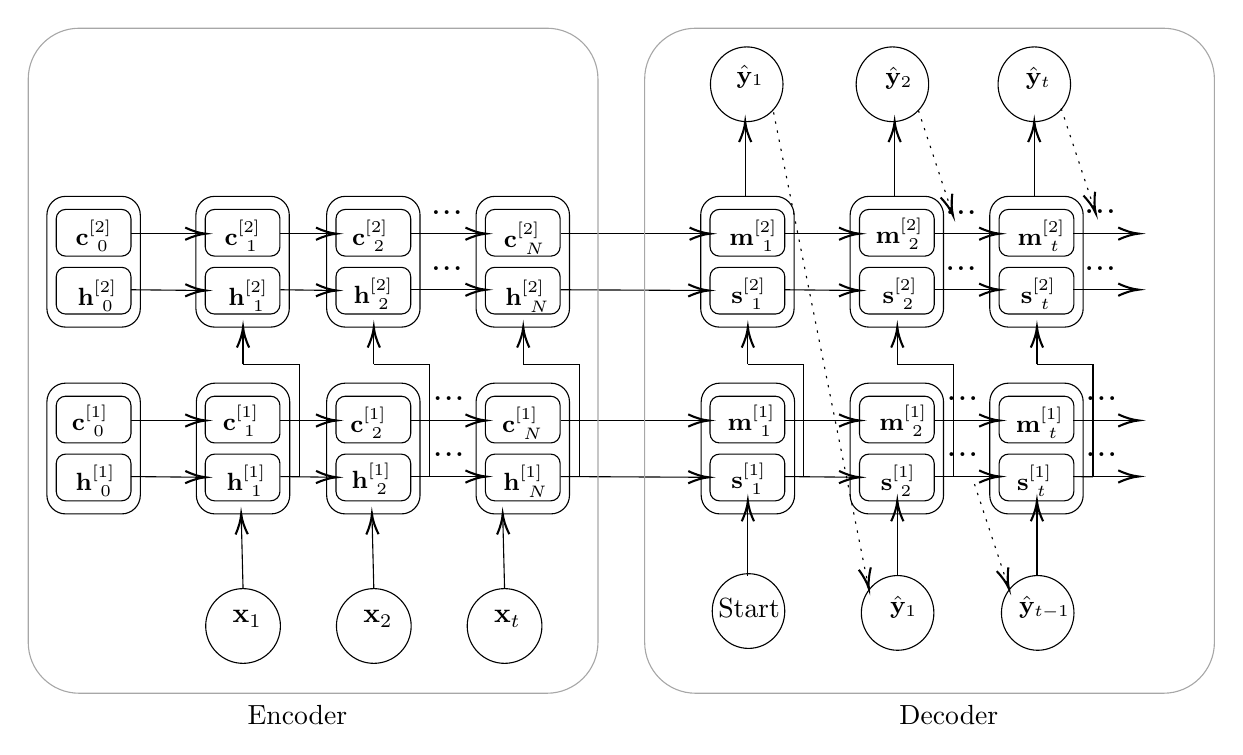
\begin{tikzpicture}[x=0.75pt,y=0.75pt,yscale=-0.9,xscale=0.9]
        %Rounded Rect [id:dp4167080735457187] 
        \draw   (95,210) .. controls (95,204.48) and (99.48,200) .. (105,200) -- (135,200) .. controls (140.52,200) and (145,204.48) .. (145,210) -- (145,260) .. controls (145,265.52) and (140.52,270) .. (135,270) -- (105,270) .. controls (99.48,270) and (95,265.52) .. (95,260) -- cycle ;
        %Rounded Rect [id:dp9346144842253596] 
        \draw   (99.75,212) .. controls (99.75,209.24) and (101.99,207) .. (104.75,207) -- (134.75,207) .. controls (137.51,207) and (139.75,209.24) .. (139.75,212) -- (139.75,227) .. controls (139.75,229.76) and (137.51,232) .. (134.75,232) -- (104.75,232) .. controls (101.99,232) and (99.75,229.76) .. (99.75,227) -- cycle ;
        %Rounded Rect [id:dp6875835908190091] 
        \draw   (99.75,243) .. controls (99.75,240.24) and (101.99,238) .. (104.75,238) -- (134.75,238) .. controls (137.51,238) and (139.75,240.24) .. (139.75,243) -- (139.75,258) .. controls (139.75,260.76) and (137.51,263) .. (134.75,263) -- (104.75,263) .. controls (101.99,263) and (99.75,260.76) .. (99.75,258) -- cycle ;
        %Shape: Ellipse [id:dp3055121979882416] 
        \draw   (100,330) .. controls (100,318.95) and (108.95,310) .. (120,310) .. controls (131.05,310) and (140,318.95) .. (140,330) .. controls (140,341.05) and (131.05,350) .. (120,350) .. controls (108.95,350) and (100,341.05) .. (100,330) -- cycle ;
        %Straight Lines [id:da9025855181913687] 
        \draw [color={rgb, 255:red, 0; green, 0; blue, 0 }  ,draw opacity=1 ]   (120,310) -- (119.05,272) ;
        \draw [shift={(119,270)}, rotate = 88.57] [color={rgb, 255:red, 0; green, 0; blue, 0 }  ,draw opacity=1 ][line width=0.75]    (10.93,-3.29) .. controls (6.95,-1.4) and (3.31,-0.3) .. (0,0) .. controls (3.31,0.3) and (6.95,1.4) .. (10.93,3.29)   ;
        %Rounded Rect [id:dp07089969288787579] 
        \draw   (15,210) .. controls (15,204.48) and (19.48,200) .. (25,200) -- (55,200) .. controls (60.52,200) and (65,204.48) .. (65,210) -- (65,260) .. controls (65,265.52) and (60.52,270) .. (55,270) -- (25,270) .. controls (19.48,270) and (15,265.52) .. (15,260) -- cycle ;
        %Rounded Rect [id:dp45824486035838286] 
        \draw   (20,212) .. controls (20,209.24) and (22.24,207) .. (25,207) -- (55,207) .. controls (57.76,207) and (60,209.24) .. (60,212) -- (60,227) .. controls (60,229.76) and (57.76,232) .. (55,232) -- (25,232) .. controls (22.24,232) and (20,229.76) .. (20,227) -- cycle ;
        %Rounded Rect [id:dp48210026138109097] 
        \draw   (20,243) .. controls (20,240.24) and (22.24,238) .. (25,238) -- (55,238) .. controls (57.76,238) and (60,240.24) .. (60,243) -- (60,258) .. controls (60,260.76) and (57.76,263) .. (55,263) -- (25,263) .. controls (22.24,263) and (20,260.76) .. (20,258) -- cycle ;
        %Straight Lines [id:da851716021162116] 
        \draw [color={rgb, 255:red, 0; green, 0; blue, 0 }  ,draw opacity=1 ]   (60,220) -- (98,220) ;
        \draw [shift={(100,220)}, rotate = 180] [color={rgb, 255:red, 0; green, 0; blue, 0 }  ,draw opacity=1 ][line width=0.75]    (10.93,-3.29) .. controls (6.95,-1.4) and (3.31,-0.3) .. (0,0) .. controls (3.31,0.3) and (6.95,1.4) .. (10.93,3.29)   ;
        %Straight Lines [id:da23842568528519448] 
        \draw [color={rgb, 255:red, 0; green, 0; blue, 0 }  ,draw opacity=1 ]   (60,250) -- (98,250.38) ;
        \draw [shift={(100,250.4)}, rotate = 180.57] [color={rgb, 255:red, 0; green, 0; blue, 0 }  ,draw opacity=1 ][line width=0.75]    (10.93,-3.29) .. controls (6.95,-1.4) and (3.31,-0.3) .. (0,0) .. controls (3.31,0.3) and (6.95,1.4) .. (10.93,3.29)   ;
        %Rounded Rect [id:dp04560159737503078] 
        \draw   (164.75,210) .. controls (164.75,204.48) and (169.23,200) .. (174.75,200) -- (204.75,200) .. controls (210.27,200) and (214.75,204.48) .. (214.75,210) -- (214.75,260) .. controls (214.75,265.52) and (210.27,270) .. (204.75,270) -- (174.75,270) .. controls (169.23,270) and (164.75,265.52) .. (164.75,260) -- cycle ;
        %Rounded Rect [id:dp08530606490144477] 
        \draw   (169.75,212) .. controls (169.75,209.24) and (171.99,207) .. (174.75,207) -- (204.75,207) .. controls (207.51,207) and (209.75,209.24) .. (209.75,212) -- (209.75,227) .. controls (209.75,229.76) and (207.51,232) .. (204.75,232) -- (174.75,232) .. controls (171.99,232) and (169.75,229.76) .. (169.75,227) -- cycle ;
        %Rounded Rect [id:dp7886901905831325] 
        \draw   (169.75,243) .. controls (169.75,240.24) and (171.99,238) .. (174.75,238) -- (204.75,238) .. controls (207.51,238) and (209.75,240.24) .. (209.75,243) -- (209.75,258) .. controls (209.75,260.76) and (207.51,263) .. (204.75,263) -- (174.75,263) .. controls (171.99,263) and (169.75,260.76) .. (169.75,258) -- cycle ;
        %Straight Lines [id:da7287683964859257] 
        \draw [color={rgb, 255:red, 0; green, 0; blue, 0 }  ,draw opacity=1 ]   (190,310) -- (189.05,272) ;
        \draw [shift={(189,270)}, rotate = 88.57] [color={rgb, 255:red, 0; green, 0; blue, 0 }  ,draw opacity=1 ][line width=0.75]    (10.93,-3.29) .. controls (6.95,-1.4) and (3.31,-0.3) .. (0,0) .. controls (3.31,0.3) and (6.95,1.4) .. (10.93,3.29)   ;
        %Straight Lines [id:da6715664171215201] 
        \draw [color={rgb, 255:red, 0; green, 0; blue, 0 }  ,draw opacity=1 ]   (140,220) -- (168,220) ;
        \draw [shift={(170,220)}, rotate = 180] [color={rgb, 255:red, 0; green, 0; blue, 0 }  ,draw opacity=1 ][line width=0.75]    (10.93,-3.29) .. controls (6.95,-1.4) and (3.31,-0.3) .. (0,0) .. controls (3.31,0.3) and (6.95,1.4) .. (10.93,3.29)   ;
        %Straight Lines [id:da6599244085959135] 
        \draw [color={rgb, 255:red, 0; green, 0; blue, 0 }  ,draw opacity=1 ]   (140,250) -- (168,250.37) ;
        \draw [shift={(170,250.4)}, rotate = 180.76] [color={rgb, 255:red, 0; green, 0; blue, 0 }  ,draw opacity=1 ][line width=0.75]    (10.93,-3.29) .. controls (6.95,-1.4) and (3.31,-0.3) .. (0,0) .. controls (3.31,0.3) and (6.95,1.4) .. (10.93,3.29)   ;
        %Rounded Rect [id:dp8902637813941603] 
        \draw   (244.75,210) .. controls (244.75,204.48) and (249.23,200) .. (254.75,200) -- (284.75,200) .. controls (290.27,200) and (294.75,204.48) .. (294.75,210) -- (294.75,260) .. controls (294.75,265.52) and (290.27,270) .. (284.75,270) -- (254.75,270) .. controls (249.23,270) and (244.75,265.52) .. (244.75,260) -- cycle ;
        %Rounded Rect [id:dp6625189643863216] 
        \draw   (249.75,212) .. controls (249.75,209.24) and (251.99,207) .. (254.75,207) -- (284.75,207) .. controls (287.51,207) and (289.75,209.24) .. (289.75,212) -- (289.75,227) .. controls (289.75,229.76) and (287.51,232) .. (284.75,232) -- (254.75,232) .. controls (251.99,232) and (249.75,229.76) .. (249.75,227) -- cycle ;
        %Rounded Rect [id:dp7778174343651048] 
        \draw   (249.75,243) .. controls (249.75,240.24) and (251.99,238) .. (254.75,238) -- (284.75,238) .. controls (287.51,238) and (289.75,240.24) .. (289.75,243) -- (289.75,258) .. controls (289.75,260.76) and (287.51,263) .. (284.75,263) -- (254.75,263) .. controls (251.99,263) and (249.75,260.76) .. (249.75,258) -- cycle ;
        %Straight Lines [id:da39906144546159594] 
        \draw [color={rgb, 255:red, 0; green, 0; blue, 0 }  ,draw opacity=1 ]   (260,310) -- (259.05,272) ;
        \draw [shift={(259,270)}, rotate = 88.57] [color={rgb, 255:red, 0; green, 0; blue, 0 }  ,draw opacity=1 ][line width=0.75]    (10.93,-3.29) .. controls (6.95,-1.4) and (3.31,-0.3) .. (0,0) .. controls (3.31,0.3) and (6.95,1.4) .. (10.93,3.29)   ;
        %Straight Lines [id:da7734816554973012] 
        \draw [color={rgb, 255:red, 0; green, 0; blue, 0 }  ,draw opacity=1 ]   (210,220) -- (248,220) ;
        \draw [shift={(250,220)}, rotate = 180] [color={rgb, 255:red, 0; green, 0; blue, 0 }  ,draw opacity=1 ][line width=0.75]    (10.93,-3.29) .. controls (6.95,-1.4) and (3.31,-0.3) .. (0,0) .. controls (3.31,0.3) and (6.95,1.4) .. (10.93,3.29)   ;
        %Straight Lines [id:da6212410028746724] 
        \draw [color={rgb, 255:red, 0; green, 0; blue, 0 }  ,draw opacity=1 ]   (210,250) -- (248,250) ;
        \draw [shift={(250,250)}, rotate = 180] [color={rgb, 255:red, 0; green, 0; blue, 0 }  ,draw opacity=1 ][line width=0.75]    (10.93,-3.29) .. controls (6.95,-1.4) and (3.31,-0.3) .. (0,0) .. controls (3.31,0.3) and (6.95,1.4) .. (10.93,3.29)   ;
        %Straight Lines [id:da6170150958930491] 
        \draw [color={rgb, 255:red, 0; green, 0; blue, 0 }  ,draw opacity=1 ]   (290,220) -- (367.25,220) ;
        \draw [shift={(369.25,220)}, rotate = 180] [color={rgb, 255:red, 0; green, 0; blue, 0 }  ,draw opacity=1 ][line width=0.75]    (10.93,-3.29) .. controls (6.95,-1.4) and (3.31,-0.3) .. (0,0) .. controls (3.31,0.3) and (6.95,1.4) .. (10.93,3.29)   ;
        %Straight Lines [id:da17036070366491862] 
        \draw [color={rgb, 255:red, 0; green, 0; blue, 0 }  ,draw opacity=1 ]   (290,250) -- (367.25,250.39) ;
        \draw [shift={(369.25,250.4)}, rotate = 180.29] [color={rgb, 255:red, 0; green, 0; blue, 0 }  ,draw opacity=1 ][line width=0.75]    (10.93,-3.29) .. controls (6.95,-1.4) and (3.31,-0.3) .. (0,0) .. controls (3.31,0.3) and (6.95,1.4) .. (10.93,3.29)   ;
        %Shape: Ellipse [id:dp921814008419761] 
        \draw   (170,330) .. controls (170,318.95) and (178.95,310) .. (190,310) .. controls (201.05,310) and (210,318.95) .. (210,330) .. controls (210,341.05) and (201.05,350) .. (190,350) .. controls (178.95,350) and (170,341.05) .. (170,330) -- cycle ;
        %Shape: Ellipse [id:dp5154518203708305] 
        \draw   (240,330) .. controls (240,318.95) and (248.95,310) .. (260,310) .. controls (271.05,310) and (280,318.95) .. (280,330) .. controls (280,341.05) and (271.05,350) .. (260,350) .. controls (248.95,350) and (240,341.05) .. (240,330) -- cycle ;
        %Rounded Rect [id:dp03092854464646244] 
        \draw   (94.75,110) .. controls (94.75,104.48) and (99.23,100) .. (104.75,100) -- (134.75,100) .. controls (140.27,100) and (144.75,104.48) .. (144.75,110) -- (144.75,160) .. controls (144.75,165.52) and (140.27,170) .. (134.75,170) -- (104.75,170) .. controls (99.23,170) and (94.75,165.52) .. (94.75,160) -- cycle ;
        %Rounded Rect [id:dp816550890492074] 
        \draw   (99.75,112) .. controls (99.75,109.24) and (101.99,107) .. (104.75,107) -- (134.75,107) .. controls (137.51,107) and (139.75,109.24) .. (139.75,112) -- (139.75,127) .. controls (139.75,129.76) and (137.51,132) .. (134.75,132) -- (104.75,132) .. controls (101.99,132) and (99.75,129.76) .. (99.75,127) -- cycle ;
        %Rounded Rect [id:dp9500665840831706] 
        \draw   (99.75,143) .. controls (99.75,140.24) and (101.99,138) .. (104.75,138) -- (134.75,138) .. controls (137.51,138) and (139.75,140.24) .. (139.75,143) -- (139.75,158) .. controls (139.75,160.76) and (137.51,163) .. (134.75,163) -- (104.75,163) .. controls (101.99,163) and (99.75,160.76) .. (99.75,158) -- cycle ;
        %Rounded Rect [id:dp3141320023119989] 
        \draw   (15,110) .. controls (15,104.48) and (19.48,100) .. (25,100) -- (55,100) .. controls (60.52,100) and (65,104.48) .. (65,110) -- (65,160) .. controls (65,165.52) and (60.52,170) .. (55,170) -- (25,170) .. controls (19.48,170) and (15,165.52) .. (15,160) -- cycle ;
        %Rounded Rect [id:dp06286358415974092] 
        \draw   (20,112) .. controls (20,109.24) and (22.24,107) .. (25,107) -- (55,107) .. controls (57.76,107) and (60,109.24) .. (60,112) -- (60,127) .. controls (60,129.76) and (57.76,132) .. (55,132) -- (25,132) .. controls (22.24,132) and (20,129.76) .. (20,127) -- cycle ;
        %Rounded Rect [id:dp09801093927348647] 
        \draw   (20,143) .. controls (20,140.24) and (22.24,138) .. (25,138) -- (55,138) .. controls (57.76,138) and (60,140.24) .. (60,143) -- (60,158) .. controls (60,160.76) and (57.76,163) .. (55,163) -- (25,163) .. controls (22.24,163) and (20,160.76) .. (20,158) -- cycle ;
        %Straight Lines [id:da026094801576276083] 
        \draw [color={rgb, 255:red, 0; green, 0; blue, 0 }  ,draw opacity=1 ]   (60,120) -- (98,120) ;
        \draw [shift={(100,120)}, rotate = 180] [color={rgb, 255:red, 0; green, 0; blue, 0 }  ,draw opacity=1 ][line width=0.75]    (10.93,-3.29) .. controls (6.95,-1.4) and (3.31,-0.3) .. (0,0) .. controls (3.31,0.3) and (6.95,1.4) .. (10.93,3.29)   ;
        %Straight Lines [id:da7209735695081336] 
        \draw [color={rgb, 255:red, 0; green, 0; blue, 0 }  ,draw opacity=1 ]   (60,150) -- (98,150.38) ;
        \draw [shift={(100,150.4)}, rotate = 180.57] [color={rgb, 255:red, 0; green, 0; blue, 0 }  ,draw opacity=1 ][line width=0.75]    (10.93,-3.29) .. controls (6.95,-1.4) and (3.31,-0.3) .. (0,0) .. controls (3.31,0.3) and (6.95,1.4) .. (10.93,3.29)   ;
        %Rounded Rect [id:dp9922570289260113] 
        \draw   (164.75,110) .. controls (164.75,104.48) and (169.23,100) .. (174.75,100) -- (204.75,100) .. controls (210.27,100) and (214.75,104.48) .. (214.75,110) -- (214.75,160) .. controls (214.75,165.52) and (210.27,170) .. (204.75,170) -- (174.75,170) .. controls (169.23,170) and (164.75,165.52) .. (164.75,160) -- cycle ;
        %Rounded Rect [id:dp9753501113257226] 
        \draw   (169.75,112) .. controls (169.75,109.24) and (171.99,107) .. (174.75,107) -- (204.75,107) .. controls (207.51,107) and (209.75,109.24) .. (209.75,112) -- (209.75,127) .. controls (209.75,129.76) and (207.51,132) .. (204.75,132) -- (174.75,132) .. controls (171.99,132) and (169.75,129.76) .. (169.75,127) -- cycle ;
        %Rounded Rect [id:dp39752964789027234] 
        \draw   (169.75,143) .. controls (169.75,140.24) and (171.99,138) .. (174.75,138) -- (204.75,138) .. controls (207.51,138) and (209.75,140.24) .. (209.75,143) -- (209.75,158) .. controls (209.75,160.76) and (207.51,163) .. (204.75,163) -- (174.75,163) .. controls (171.99,163) and (169.75,160.76) .. (169.75,158) -- cycle ;
        %Straight Lines [id:da7201454739572428] 
        \draw [color={rgb, 255:red, 0; green, 0; blue, 0 }  ,draw opacity=1 ]   (140,120) -- (168,120) ;
        \draw [shift={(170,120)}, rotate = 180] [color={rgb, 255:red, 0; green, 0; blue, 0 }  ,draw opacity=1 ][line width=0.75]    (10.93,-3.29) .. controls (6.95,-1.4) and (3.31,-0.3) .. (0,0) .. controls (3.31,0.3) and (6.95,1.4) .. (10.93,3.29)   ;
        %Straight Lines [id:da714248693226855] 
        \draw [color={rgb, 255:red, 0; green, 0; blue, 0 }  ,draw opacity=1 ]   (140,150) -- (168,150.37) ;
        \draw [shift={(170,150.4)}, rotate = 180.76] [color={rgb, 255:red, 0; green, 0; blue, 0 }  ,draw opacity=1 ][line width=0.75]    (10.93,-3.29) .. controls (6.95,-1.4) and (3.31,-0.3) .. (0,0) .. controls (3.31,0.3) and (6.95,1.4) .. (10.93,3.29)   ;
        %Rounded Rect [id:dp9710143758385796] 
        \draw   (244.75,110) .. controls (244.75,104.48) and (249.23,100) .. (254.75,100) -- (284.75,100) .. controls (290.27,100) and (294.75,104.48) .. (294.75,110) -- (294.75,160) .. controls (294.75,165.52) and (290.27,170) .. (284.75,170) -- (254.75,170) .. controls (249.23,170) and (244.75,165.52) .. (244.75,160) -- cycle ;
        %Rounded Rect [id:dp6076792282358365] 
        \draw   (249.75,112) .. controls (249.75,109.24) and (251.99,107) .. (254.75,107) -- (284.75,107) .. controls (287.51,107) and (289.75,109.24) .. (289.75,112) -- (289.75,127) .. controls (289.75,129.76) and (287.51,132) .. (284.75,132) -- (254.75,132) .. controls (251.99,132) and (249.75,129.76) .. (249.75,127) -- cycle ;
        %Rounded Rect [id:dp8301870485368747] 
        \draw   (249.75,143) .. controls (249.75,140.24) and (251.99,138) .. (254.75,138) -- (284.75,138) .. controls (287.51,138) and (289.75,140.24) .. (289.75,143) -- (289.75,158) .. controls (289.75,160.76) and (287.51,163) .. (284.75,163) -- (254.75,163) .. controls (251.99,163) and (249.75,160.76) .. (249.75,158) -- cycle ;
        %Straight Lines [id:da18021147009414817] 
        \draw [color={rgb, 255:red, 0; green, 0; blue, 0 }  ,draw opacity=1 ]   (210,120) -- (248,120) ;
        \draw [shift={(250,120)}, rotate = 180] [color={rgb, 255:red, 0; green, 0; blue, 0 }  ,draw opacity=1 ][line width=0.75]    (10.93,-3.29) .. controls (6.95,-1.4) and (3.31,-0.3) .. (0,0) .. controls (3.31,0.3) and (6.95,1.4) .. (10.93,3.29)   ;
        %Straight Lines [id:da9792801142158605] 
        \draw [color={rgb, 255:red, 0; green, 0; blue, 0 }  ,draw opacity=1 ]   (210,150) -- (248,150) ;
        \draw [shift={(250,150)}, rotate = 180] [color={rgb, 255:red, 0; green, 0; blue, 0 }  ,draw opacity=1 ][line width=0.75]    (10.93,-3.29) .. controls (6.95,-1.4) and (3.31,-0.3) .. (0,0) .. controls (3.31,0.3) and (6.95,1.4) .. (10.93,3.29)   ;
        %Straight Lines [id:da09217962764014365] 
        \draw [color={rgb, 255:red, 0; green, 0; blue, 0 }  ,draw opacity=1 ]   (290,120) -- (368,120) ;
        \draw [shift={(370,120)}, rotate = 180] [color={rgb, 255:red, 0; green, 0; blue, 0 }  ,draw opacity=1 ][line width=0.75]    (10.93,-3.29) .. controls (6.95,-1.4) and (3.31,-0.3) .. (0,0) .. controls (3.31,0.3) and (6.95,1.4) .. (10.93,3.29)   ;
        %Straight Lines [id:da07024764866360234] 
        \draw [color={rgb, 255:red, 0; green, 0; blue, 0 }  ,draw opacity=1 ]   (290,150) -- (367.25,150.39) ;
        \draw [shift={(369.25,150.4)}, rotate = 180.29] [color={rgb, 255:red, 0; green, 0; blue, 0 }  ,draw opacity=1 ][line width=0.75]    (10.93,-3.29) .. controls (6.95,-1.4) and (3.31,-0.3) .. (0,0) .. controls (3.31,0.3) and (6.95,1.4) .. (10.93,3.29)   ;
        %Straight Lines [id:da8792682771837725] 
        \draw    (150,250.2) -- (150,190) ;
        %Straight Lines [id:da2634240032707502] 
        \draw    (120,190) -- (150,190) ;
        %Straight Lines [id:da12484928851738863] 
        \draw    (120,190) -- (120,172) ;
        \draw [shift={(120,170)}, rotate = 90] [color={rgb, 255:red, 0; green, 0; blue, 0 }  ][line width=0.75]    (10.93,-3.29) .. controls (6.95,-1.4) and (3.31,-0.3) .. (0,0) .. controls (3.31,0.3) and (6.95,1.4) .. (10.93,3.29)   ;
        %Straight Lines [id:da5759992375631084] 
        \draw    (220,250.2) -- (220,190) ;
        %Straight Lines [id:da5103327101821591] 
        \draw    (190,190) -- (220,190) ;
        %Straight Lines [id:da7509876273419771] 
        \draw    (190,190) -- (190,172) ;
        \draw [shift={(190,170)}, rotate = 90] [color={rgb, 255:red, 0; green, 0; blue, 0 }  ][line width=0.75]    (10.93,-3.29) .. controls (6.95,-1.4) and (3.31,-0.3) .. (0,0) .. controls (3.31,0.3) and (6.95,1.4) .. (10.93,3.29)   ;
        %Straight Lines [id:da15793149664296036] 
        \draw    (270,190) -- (300,190) ;
        %Straight Lines [id:da4796232669148728] 
        \draw    (270,190) -- (270,172) ;
        \draw [shift={(270,170)}, rotate = 90] [color={rgb, 255:red, 0; green, 0; blue, 0 }  ][line width=0.75]    (10.93,-3.29) .. controls (6.95,-1.4) and (3.31,-0.3) .. (0,0) .. controls (3.31,0.3) and (6.95,1.4) .. (10.93,3.29)   ;
        %Straight Lines [id:da700877547716785] 
        \draw    (300,250.2) -- (300,190) ;
        %Rounded Rect [id:dp8674888716756768] 
        \draw   (365.25,210) .. controls (365.25,204.48) and (369.73,200) .. (375.25,200) -- (405.25,200) .. controls (410.77,200) and (415.25,204.48) .. (415.25,210) -- (415.25,260) .. controls (415.25,265.52) and (410.77,270) .. (405.25,270) -- (375.25,270) .. controls (369.73,270) and (365.25,265.52) .. (365.25,260) -- cycle ;
        %Rounded Rect [id:dp5489391539785766] 
        \draw   (370,212) .. controls (370,209.24) and (372.24,207) .. (375,207) -- (405,207) .. controls (407.76,207) and (410,209.24) .. (410,212) -- (410,227) .. controls (410,229.76) and (407.76,232) .. (405,232) -- (375,232) .. controls (372.24,232) and (370,229.76) .. (370,227) -- cycle ;
        %Rounded Rect [id:dp5963099944409156] 
        \draw   (370,243) .. controls (370,240.24) and (372.24,238) .. (375,238) -- (405,238) .. controls (407.76,238) and (410,240.24) .. (410,243) -- (410,258) .. controls (410,260.76) and (407.76,263) .. (405,263) -- (375,263) .. controls (372.24,263) and (370,260.76) .. (370,258) -- cycle ;
        %Straight Lines [id:da911979939972424] 
        \draw [color={rgb, 255:red, 0; green, 0; blue, 0 }  ,draw opacity=1 ]   (388.82,100) -- (388.82,66) -- (388.82,62) ;
        \draw [shift={(388.82,60)}, rotate = 90] [color={rgb, 255:red, 0; green, 0; blue, 0 }  ,draw opacity=1 ][line width=0.75]    (10.93,-3.29) .. controls (6.95,-1.4) and (3.31,-0.3) .. (0,0) .. controls (3.31,0.3) and (6.95,1.4) .. (10.93,3.29)   ;
        %Rounded Rect [id:dp7221083753374034] 
        \draw   (445,210) .. controls (445,204.48) and (449.48,200) .. (455,200) -- (485,200) .. controls (490.52,200) and (495,204.48) .. (495,210) -- (495,260) .. controls (495,265.52) and (490.52,270) .. (485,270) -- (455,270) .. controls (449.48,270) and (445,265.52) .. (445,260) -- cycle ;
        %Rounded Rect [id:dp36860252170123875] 
        \draw   (450,212) .. controls (450,209.24) and (452.24,207) .. (455,207) -- (485,207) .. controls (487.76,207) and (490,209.24) .. (490,212) -- (490,227) .. controls (490,229.76) and (487.76,232) .. (485,232) -- (455,232) .. controls (452.24,232) and (450,229.76) .. (450,227) -- cycle ;
        %Rounded Rect [id:dp6114065023247515] 
        \draw   (450,243) .. controls (450,240.24) and (452.24,238) .. (455,238) -- (485,238) .. controls (487.76,238) and (490,240.24) .. (490,243) -- (490,258) .. controls (490,260.76) and (487.76,263) .. (485,263) -- (455,263) .. controls (452.24,263) and (450,260.76) .. (450,258) -- cycle ;
        %Straight Lines [id:da6816491393136734] 
        \draw [color={rgb, 255:red, 0; green, 0; blue, 0 }  ,draw opacity=1 ]   (468.82,100) -- (468.82,66) -- (468.82,62) ;
        \draw [shift={(468.82,60)}, rotate = 90] [color={rgb, 255:red, 0; green, 0; blue, 0 }  ,draw opacity=1 ][line width=0.75]    (10.93,-3.29) .. controls (6.95,-1.4) and (3.31,-0.3) .. (0,0) .. controls (3.31,0.3) and (6.95,1.4) .. (10.93,3.29)   ;
        %Rounded Rect [id:dp509214694654305] 
        \draw   (519.75,210) .. controls (519.75,204.48) and (524.23,200) .. (529.75,200) -- (559.75,200) .. controls (565.27,200) and (569.75,204.48) .. (569.75,210) -- (569.75,260) .. controls (569.75,265.52) and (565.27,270) .. (559.75,270) -- (529.75,270) .. controls (524.23,270) and (519.75,265.52) .. (519.75,260) -- cycle ;
        %Rounded Rect [id:dp41118491999009565] 
        \draw   (524.75,212) .. controls (524.75,209.24) and (526.99,207) .. (529.75,207) -- (559.75,207) .. controls (562.51,207) and (564.75,209.24) .. (564.75,212) -- (564.75,227) .. controls (564.75,229.76) and (562.51,232) .. (559.75,232) -- (529.75,232) .. controls (526.99,232) and (524.75,229.76) .. (524.75,227) -- cycle ;
        %Rounded Rect [id:dp04750143326593914] 
        \draw   (524.75,243) .. controls (524.75,240.24) and (526.99,238) .. (529.75,238) -- (559.75,238) .. controls (562.51,238) and (564.75,240.24) .. (564.75,243) -- (564.75,258) .. controls (564.75,260.76) and (562.51,263) .. (559.75,263) -- (529.75,263) .. controls (526.99,263) and (524.75,260.76) .. (524.75,258) -- cycle ;
        %Straight Lines [id:da8817473076349263] 
        \draw [color={rgb, 255:red, 0; green, 0; blue, 0 }  ,draw opacity=1 ]   (543.57,100) -- (543.57,66) -- (543.57,62) ;
        \draw [shift={(543.57,60)}, rotate = 90] [color={rgb, 255:red, 0; green, 0; blue, 0 }  ,draw opacity=1 ][line width=0.75]    (10.93,-3.29) .. controls (6.95,-1.4) and (3.31,-0.3) .. (0,0) .. controls (3.31,0.3) and (6.95,1.4) .. (10.93,3.29)   ;
        %Straight Lines [id:da27286644665918924] 
        \draw [color={rgb, 255:red, 0; green, 0; blue, 0 }  ,draw opacity=1 ]   (410,220) -- (448,220) ;
        \draw [shift={(450,220)}, rotate = 180] [color={rgb, 255:red, 0; green, 0; blue, 0 }  ,draw opacity=1 ][line width=0.75]    (10.93,-3.29) .. controls (6.95,-1.4) and (3.31,-0.3) .. (0,0) .. controls (3.31,0.3) and (6.95,1.4) .. (10.93,3.29)   ;
        %Straight Lines [id:da9479965742141365] 
        \draw [color={rgb, 255:red, 0; green, 0; blue, 0 }  ,draw opacity=1 ]   (410,250) -- (448,250.38) ;
        \draw [shift={(450,250.4)}, rotate = 180.57] [color={rgb, 255:red, 0; green, 0; blue, 0 }  ,draw opacity=1 ][line width=0.75]    (10.93,-3.29) .. controls (6.95,-1.4) and (3.31,-0.3) .. (0,0) .. controls (3.31,0.3) and (6.95,1.4) .. (10.93,3.29)   ;
        %Rounded Rect [id:dp19540509121782024] 
        \draw   (365,110) .. controls (365,104.48) and (369.48,100) .. (375,100) -- (405,100) .. controls (410.52,100) and (415,104.48) .. (415,110) -- (415,160) .. controls (415,165.52) and (410.52,170) .. (405,170) -- (375,170) .. controls (369.48,170) and (365,165.52) .. (365,160) -- cycle ;
        %Rounded Rect [id:dp2762867928089998] 
        \draw   (370,112) .. controls (370,109.24) and (372.24,107) .. (375,107) -- (405,107) .. controls (407.76,107) and (410,109.24) .. (410,112) -- (410,127) .. controls (410,129.76) and (407.76,132) .. (405,132) -- (375,132) .. controls (372.24,132) and (370,129.76) .. (370,127) -- cycle ;
        %Rounded Rect [id:dp9587780841664757] 
        \draw   (370,143) .. controls (370,140.24) and (372.24,138) .. (375,138) -- (405,138) .. controls (407.76,138) and (410,140.24) .. (410,143) -- (410,158) .. controls (410,160.76) and (407.76,163) .. (405,163) -- (375,163) .. controls (372.24,163) and (370,160.76) .. (370,158) -- cycle ;
        %Rounded Rect [id:dp5296850448101615] 
        \draw   (445,110) .. controls (445,104.48) and (449.48,100) .. (455,100) -- (485,100) .. controls (490.52,100) and (495,104.48) .. (495,110) -- (495,160) .. controls (495,165.52) and (490.52,170) .. (485,170) -- (455,170) .. controls (449.48,170) and (445,165.52) .. (445,160) -- cycle ;
        %Rounded Rect [id:dp7925349138834241] 
        \draw   (450,112) .. controls (450,109.24) and (452.24,107) .. (455,107) -- (485,107) .. controls (487.76,107) and (490,109.24) .. (490,112) -- (490,127) .. controls (490,129.76) and (487.76,132) .. (485,132) -- (455,132) .. controls (452.24,132) and (450,129.76) .. (450,127) -- cycle ;
        %Rounded Rect [id:dp10913626409203814] 
        \draw   (450,143) .. controls (450,140.24) and (452.24,138) .. (455,138) -- (485,138) .. controls (487.76,138) and (490,140.24) .. (490,143) -- (490,158) .. controls (490,160.76) and (487.76,163) .. (485,163) -- (455,163) .. controls (452.24,163) and (450,160.76) .. (450,158) -- cycle ;
        %Rounded Rect [id:dp23474579373402982] 
        \draw   (519.75,110) .. controls (519.75,104.48) and (524.23,100) .. (529.75,100) -- (559.75,100) .. controls (565.27,100) and (569.75,104.48) .. (569.75,110) -- (569.75,160) .. controls (569.75,165.52) and (565.27,170) .. (559.75,170) -- (529.75,170) .. controls (524.23,170) and (519.75,165.52) .. (519.75,160) -- cycle ;
        %Rounded Rect [id:dp08285224899170052] 
        \draw   (524.75,112) .. controls (524.75,109.24) and (526.99,107) .. (529.75,107) -- (559.75,107) .. controls (562.51,107) and (564.75,109.24) .. (564.75,112) -- (564.75,127) .. controls (564.75,129.76) and (562.51,132) .. (559.75,132) -- (529.75,132) .. controls (526.99,132) and (524.75,129.76) .. (524.75,127) -- cycle ;
        %Rounded Rect [id:dp09356096334165964] 
        \draw   (524.75,143) .. controls (524.75,140.24) and (526.99,138) .. (529.75,138) -- (559.75,138) .. controls (562.51,138) and (564.75,140.24) .. (564.75,143) -- (564.75,158) .. controls (564.75,160.76) and (562.51,163) .. (559.75,163) -- (529.75,163) .. controls (526.99,163) and (524.75,160.76) .. (524.75,158) -- cycle ;
        %Straight Lines [id:da2630583353195102] 
        \draw [color={rgb, 255:red, 0; green, 0; blue, 0 }  ,draw opacity=1 ]   (410,120) -- (448,120) ;
        \draw [shift={(450,120)}, rotate = 180] [color={rgb, 255:red, 0; green, 0; blue, 0 }  ,draw opacity=1 ][line width=0.75]    (10.93,-3.29) .. controls (6.95,-1.4) and (3.31,-0.3) .. (0,0) .. controls (3.31,0.3) and (6.95,1.4) .. (10.93,3.29)   ;
        %Straight Lines [id:da9003673432635384] 
        \draw [color={rgb, 255:red, 0; green, 0; blue, 0 }  ,draw opacity=1 ]   (410,150) -- (448,150.38) ;
        \draw [shift={(450,150.4)}, rotate = 180.57] [color={rgb, 255:red, 0; green, 0; blue, 0 }  ,draw opacity=1 ][line width=0.75]    (10.93,-3.29) .. controls (6.95,-1.4) and (3.31,-0.3) .. (0,0) .. controls (3.31,0.3) and (6.95,1.4) .. (10.93,3.29)   ;
        %Straight Lines [id:da6304538683356946] 
        \draw    (420.25,250.2) -- (420.25,190) ;
        %Straight Lines [id:da8370681679149368] 
        \draw    (390.25,190) -- (420.25,190) ;
        %Straight Lines [id:da36413170867480615] 
        \draw    (390.25,190) -- (390.25,172) ;
        \draw [shift={(390.25,170)}, rotate = 90] [color={rgb, 255:red, 0; green, 0; blue, 0 }  ][line width=0.75]    (10.93,-3.29) .. controls (6.95,-1.4) and (3.31,-0.3) .. (0,0) .. controls (3.31,0.3) and (6.95,1.4) .. (10.93,3.29)   ;
        %Straight Lines [id:da02263779133221222] 
        \draw    (500.25,250.2) -- (500.25,190) ;
        %Straight Lines [id:da6321066586201223] 
        \draw    (470.25,190) -- (500.25,190) ;
        %Straight Lines [id:da9741545158763674] 
        \draw    (470.25,190) -- (470.25,172) ;
        \draw [shift={(470.25,170)}, rotate = 90] [color={rgb, 255:red, 0; green, 0; blue, 0 }  ][line width=0.75]    (10.93,-3.29) .. controls (6.95,-1.4) and (3.31,-0.3) .. (0,0) .. controls (3.31,0.3) and (6.95,1.4) .. (10.93,3.29)   ;
        %Straight Lines [id:da47873868152464216] 
        \draw    (575,250.2) -- (575,190) ;
        %Straight Lines [id:da6668557121227057] 
        \draw    (545,190) -- (575,190) ;
        %Straight Lines [id:da12904452588003146] 
        \draw    (545,190) -- (545,172) ;
        \draw [shift={(545,170)}, rotate = 90] [color={rgb, 255:red, 0; green, 0; blue, 0 }  ][line width=0.75]    (10.93,-3.29) .. controls (6.95,-1.4) and (3.31,-0.3) .. (0,0) .. controls (3.31,0.3) and (6.95,1.4) .. (10.93,3.29)   ;
        %Straight Lines [id:da7293210834974657] 
        \draw [color={rgb, 255:red, 0; green, 0; blue, 0 }  ,draw opacity=1 ]   (490,220) -- (523,220) ;
        \draw [shift={(525,220)}, rotate = 180] [color={rgb, 255:red, 0; green, 0; blue, 0 }  ,draw opacity=1 ][line width=0.75]    (10.93,-3.29) .. controls (6.95,-1.4) and (3.31,-0.3) .. (0,0) .. controls (3.31,0.3) and (6.95,1.4) .. (10.93,3.29)   ;
        %Straight Lines [id:da1064022544729053] 
        \draw [color={rgb, 255:red, 0; green, 0; blue, 0 }  ,draw opacity=1 ]   (490,250) -- (523,250) ;
        \draw [shift={(525,250)}, rotate = 180] [color={rgb, 255:red, 0; green, 0; blue, 0 }  ,draw opacity=1 ][line width=0.75]    (10.93,-3.29) .. controls (6.95,-1.4) and (3.31,-0.3) .. (0,0) .. controls (3.31,0.3) and (6.95,1.4) .. (10.93,3.29)   ;
        %Straight Lines [id:da07130857733309437] 
        \draw [color={rgb, 255:red, 0; green, 0; blue, 0 }  ,draw opacity=1 ]   (490,120) -- (523,120) ;
        \draw [shift={(525,120)}, rotate = 180] [color={rgb, 255:red, 0; green, 0; blue, 0 }  ,draw opacity=1 ][line width=0.75]    (10.93,-3.29) .. controls (6.95,-1.4) and (3.31,-0.3) .. (0,0) .. controls (3.31,0.3) and (6.95,1.4) .. (10.93,3.29)   ;
        %Straight Lines [id:da7312641973991214] 
        \draw [color={rgb, 255:red, 0; green, 0; blue, 0 }  ,draw opacity=1 ]   (490,150) -- (523,150) ;
        \draw [shift={(525,150)}, rotate = 180] [color={rgb, 255:red, 0; green, 0; blue, 0 }  ,draw opacity=1 ][line width=0.75]    (10.93,-3.29) .. controls (6.95,-1.4) and (3.31,-0.3) .. (0,0) .. controls (3.31,0.3) and (6.95,1.4) .. (10.93,3.29)   ;
        %Straight Lines [id:da9300102498701175] 
        \draw    (565,250) -- (575,250.2) ;
        %Rounded Rect [id:dp3317617565588511] 
        \draw  [color={rgb, 255:red, 167; green, 167; blue, 167 }  ,draw opacity=1 ] (5,37.26) .. controls (5,22.2) and (17.2,10) .. (32.26,10) -- (282.74,10) .. controls (297.8,10) and (310,22.2) .. (310,37.26) -- (310,338.74) .. controls (310,353.8) and (297.8,366) .. (282.74,366) -- (32.26,366) .. controls (17.2,366) and (5,353.8) .. (5,338.74) -- cycle ;
        %Rounded Rect [id:dp5783177244986819] 
        \draw  [color={rgb, 255:red, 167; green, 167; blue, 167 }  ,draw opacity=1 ] (335,37.26) .. controls (335,22.2) and (347.2,10) .. (362.26,10) -- (612.74,10) .. controls (627.8,10) and (640,22.2) .. (640,37.26) -- (640,338.74) .. controls (640,353.8) and (627.8,366) .. (612.74,366) -- (362.26,366) .. controls (347.2,366) and (335,353.8) .. (335,338.74) -- cycle ;
        %Shape: Ellipse [id:dp7733394302286176] 
        \draw   (448.22,40) .. controls (448.22,28.95) and (456.91,20) .. (467.63,20) .. controls (478.35,20) and (487.04,28.95) .. (487.04,40) .. controls (487.04,51.05) and (478.35,60) .. (467.63,60) .. controls (456.91,60) and (448.22,51.05) .. (448.22,40) -- cycle ;
        %Shape: Ellipse [id:dp6556072395259707] 
        \draw   (524.18,40) .. controls (524.18,28.95) and (532.87,20) .. (543.59,20) .. controls (554.31,20) and (563,28.95) .. (563,40) .. controls (563,51.05) and (554.31,60) .. (543.59,60) .. controls (532.87,60) and (524.18,51.05) .. (524.18,40) -- cycle ;
        %Shape: Ellipse [id:dp3170085190999692] 
        \draw   (370.22,40) .. controls (370.22,28.95) and (378.91,20) .. (389.64,20) .. controls (400.36,20) and (409.05,28.95) .. (409.05,40) .. controls (409.05,51.05) and (400.36,60) .. (389.64,60) .. controls (378.91,60) and (370.22,51.05) .. (370.22,40) -- cycle ;
        %Straight Lines [id:da1470169361742475] 
        \draw [color={rgb, 255:red, 0; green, 0; blue, 0 }  ,draw opacity=1 ]   (390.25,303) -- (390.25,269) -- (390.25,265) ;
        \draw [shift={(390.25,263)}, rotate = 90] [color={rgb, 255:red, 0; green, 0; blue, 0 }  ,draw opacity=1 ][line width=0.75]    (10.93,-3.29) .. controls (6.95,-1.4) and (3.31,-0.3) .. (0,0) .. controls (3.31,0.3) and (6.95,1.4) .. (10.93,3.29)   ;
        %Straight Lines [id:da41901171346149146] 
        \draw [color={rgb, 255:red, 0; green, 0; blue, 0 }  ,draw opacity=1 ]   (470.25,303) -- (470.25,269) -- (470.25,265) ;
        \draw [shift={(470.25,263)}, rotate = 90] [color={rgb, 255:red, 0; green, 0; blue, 0 }  ,draw opacity=1 ][line width=0.75]    (10.93,-3.29) .. controls (6.95,-1.4) and (3.31,-0.3) .. (0,0) .. controls (3.31,0.3) and (6.95,1.4) .. (10.93,3.29)   ;
        %Straight Lines [id:da9442497190844032] 
        \draw [color={rgb, 255:red, 0; green, 0; blue, 0 }  ,draw opacity=1 ]   (545,303) -- (545,269) -- (545,265) ;
        \draw [shift={(545,263)}, rotate = 90] [color={rgb, 255:red, 0; green, 0; blue, 0 }  ,draw opacity=1 ][line width=0.75]    (10.93,-3.29) .. controls (6.95,-1.4) and (3.31,-0.3) .. (0,0) .. controls (3.31,0.3) and (6.95,1.4) .. (10.93,3.29)   ;
        %Shape: Ellipse [id:dp26075433324765007] 
        \draw   (451,323) .. controls (451,311.95) and (459.69,303) .. (470.41,303) .. controls (481.13,303) and (489.82,311.95) .. (489.82,323) .. controls (489.82,334.05) and (481.13,343) .. (470.41,343) .. controls (459.69,343) and (451,334.05) .. (451,323) -- cycle ;
        %Shape: Ellipse [id:dp9999850289764194] 
        \draw   (526,323) .. controls (526,311.95) and (534.69,303) .. (545.41,303) .. controls (556.13,303) and (564.82,311.95) .. (564.82,323) .. controls (564.82,334.05) and (556.13,343) .. (545.41,343) .. controls (534.69,343) and (526,334.05) .. (526,323) -- cycle ;
        %Shape: Ellipse [id:dp9467729465080421] 
        \draw   (371.18,322) .. controls (371.18,310.95) and (379.87,302) .. (390.59,302) .. controls (401.31,302) and (410,310.95) .. (410,322) .. controls (410,333.05) and (401.31,342) .. (390.59,342) .. controls (379.87,342) and (371.18,333.05) .. (371.18,322) -- cycle ;
        %Straight Lines [id:da027983118369862225] 
        \draw  [dash pattern={on 0.84pt off 2.51pt}]  (404,55) -- (454.61,308.04) ;
        \draw [shift={(455,310)}, rotate = 258.69] [color={rgb, 255:red, 0; green, 0; blue, 0 }  ][line width=0.75]    (10.93,-3.29) .. controls (6.95,-1.4) and (3.31,-0.3) .. (0,0) .. controls (3.31,0.3) and (6.95,1.4) .. (10.93,3.29)   ;
        %Straight Lines [id:da421370449385543] 
        \draw  [dash pattern={on 0.84pt off 2.51pt}]  (481.55,54.04) -- (499.37,108.1) ;
        \draw [shift={(500,110)}, rotate = 251.75] [color={rgb, 255:red, 0; green, 0; blue, 0 }  ][line width=0.75]    (10.93,-3.29) .. controls (6.95,-1.4) and (3.31,-0.3) .. (0,0) .. controls (3.31,0.3) and (6.95,1.4) .. (10.93,3.29)   ;
        %Straight Lines [id:da7826555051462878] 
        \draw [color={rgb, 255:red, 0; green, 0; blue, 0 }  ,draw opacity=1 ]   (564.45,219.96) -- (597.45,219.96) ;
        \draw [shift={(599.45,219.96)}, rotate = 180] [color={rgb, 255:red, 0; green, 0; blue, 0 }  ,draw opacity=1 ][line width=0.75]    (10.93,-3.29) .. controls (6.95,-1.4) and (3.31,-0.3) .. (0,0) .. controls (3.31,0.3) and (6.95,1.4) .. (10.93,3.29)   ;
        %Straight Lines [id:da45270197344696106] 
        \draw [color={rgb, 255:red, 0; green, 0; blue, 0 }  ,draw opacity=1 ]   (564.45,249.96) -- (597.45,249.96) ;
        \draw [shift={(599.45,249.96)}, rotate = 180] [color={rgb, 255:red, 0; green, 0; blue, 0 }  ,draw opacity=1 ][line width=0.75]    (10.93,-3.29) .. controls (6.95,-1.4) and (3.31,-0.3) .. (0,0) .. controls (3.31,0.3) and (6.95,1.4) .. (10.93,3.29)   ;
        %Straight Lines [id:da6533397571061048] 
        \draw [color={rgb, 255:red, 0; green, 0; blue, 0 }  ,draw opacity=1 ]   (564.45,119.96) -- (597.45,119.96) ;
        \draw [shift={(599.45,119.96)}, rotate = 180] [color={rgb, 255:red, 0; green, 0; blue, 0 }  ,draw opacity=1 ][line width=0.75]    (10.93,-3.29) .. controls (6.95,-1.4) and (3.31,-0.3) .. (0,0) .. controls (3.31,0.3) and (6.95,1.4) .. (10.93,3.29)   ;
        %Straight Lines [id:da5060182014403987] 
        \draw [color={rgb, 255:red, 0; green, 0; blue, 0 }  ,draw opacity=1 ]   (564.45,149.96) -- (597.45,149.96) ;
        \draw [shift={(599.45,149.96)}, rotate = 180] [color={rgb, 255:red, 0; green, 0; blue, 0 }  ,draw opacity=1 ][line width=0.75]    (10.93,-3.29) .. controls (6.95,-1.4) and (3.31,-0.3) .. (0,0) .. controls (3.31,0.3) and (6.95,1.4) .. (10.93,3.29)   ;
        %Straight Lines [id:da887931619832435] 
        \draw  [dash pattern={on 0.84pt off 2.51pt}]  (511.55,254.04) -- (529.37,308.1) ;
        \draw [shift={(530,310)}, rotate = 251.75] [color={rgb, 255:red, 0; green, 0; blue, 0 }  ][line width=0.75]    (10.93,-3.29) .. controls (6.95,-1.4) and (3.31,-0.3) .. (0,0) .. controls (3.31,0.3) and (6.95,1.4) .. (10.93,3.29)   ;
        %Straight Lines [id:da904024081259367] 
        \draw  [dash pattern={on 0.84pt off 2.51pt}]  (558,53) -- (575.83,107.06) ;
        \draw [shift={(576.45,108.96)}, rotate = 251.75] [color={rgb, 255:red, 0; green, 0; blue, 0 }  ][line width=0.75]    (10.93,-3.29) .. controls (6.95,-1.4) and (3.31,-0.3) .. (0,0) .. controls (3.31,0.3) and (6.95,1.4) .. (10.93,3.29)   ;

        % Text Node
        \draw (113,320.4) node [anchor=north west][inner sep=0.75pt]  [font=\normalsize]  {$\mathbf{x}_{1}$};
        % Text Node
        \draw (220,206) node [anchor=north west][inner sep=0.75pt]  [font=\Large] [align=left] {...};
        % Text Node
        \draw (220,236) node [anchor=north west][inner sep=0.75pt]  [font=\Large] [align=left] {...};
        % Text Node
        \draw (183,320.4) node [anchor=north west][inner sep=0.75pt]  [font=\normalsize]  {$\mathbf{x}_{2}$};
        % Text Node
        \draw (253,320.4) node [anchor=north west][inner sep=0.75pt]  [font=\normalsize]  {$\mathbf{x}_{t}$};
        % Text Node
        \draw (110.75,143.4) node [anchor=north west][inner sep=0.75pt]  [font=\small]  {$\mathbf{h}_{\ 1}^{[ 2]}$};
        % Text Node
        \draw (108.75,111.4) node [anchor=north west][inner sep=0.75pt]  [font=\small]  {$\mathbf{c}_{\ 1}^{[ 2]}$};
        % Text Node
        \draw (30,143.4) node [anchor=north west][inner sep=0.75pt]  [font=\small]  {$\mathbf{h}_{\ 0}^{[ 2]}$};
        % Text Node
        \draw (29,111.4) node [anchor=north west][inner sep=0.75pt]  [font=\small]  {$\mathbf{c}_{\ 0}^{[ 2]}$};
        % Text Node
        \draw (219,106) node [anchor=north west][inner sep=0.75pt]  [font=\Large] [align=left] {...};
        % Text Node
        \draw (219,136) node [anchor=north west][inner sep=0.75pt]  [font=\Large] [align=left] {...};
        % Text Node
        \draw (177.75,142.4) node [anchor=north west][inner sep=0.75pt]  [font=\small]  {$\mathbf{h}_{\ 2}^{[ 2]}$};
        % Text Node
        \draw (177,111.4) node [anchor=north west][inner sep=0.75pt]  [font=\small]  {$\mathbf{c}_{\ 2}^{[ 2]}$};
        % Text Node
        \draw (259,143.4) node [anchor=north west][inner sep=0.75pt]  [font=\small]  {$\mathbf{h}_{\ N}^{[ 2]}$};
        % Text Node
        \draw (258.25,112.4) node [anchor=north west][inner sep=0.75pt]  [font=\small]  {$\mathbf{c}_{\ N}^{[ 2]}$};
        % Text Node
        \draw (109.75,242.4) node [anchor=north west][inner sep=0.75pt]  [font=\small]  {$\mathbf{h}_{\ 1}^{[ 1]}$};
        % Text Node
        \draw (107.75,210.4) node [anchor=north west][inner sep=0.75pt]  [font=\small]  {$\mathbf{c}_{\ 1}^{[ 1]}$};
        % Text Node
        \draw (29,242.4) node [anchor=north west][inner sep=0.75pt]  [font=\small]  {$\mathbf{h}_{\ 0}^{[ 1]}$};
        % Text Node
        \draw (27,210.4) node [anchor=north west][inner sep=0.75pt]  [font=\small]  {$\mathbf{c}_{\ 0}^{[ 1]}$};
        % Text Node
        \draw (176.75,241.4) node [anchor=north west][inner sep=0.75pt]  [font=\small]  {$\mathbf{h}_{\ 2}^{[ 1]}$};
        % Text Node
        \draw (176,211.4) node [anchor=north west][inner sep=0.75pt]  [font=\small]  {$\mathbf{c}_{\ 2}^{[ 1]}$};
        % Text Node
        \draw (258,242.4) node [anchor=north west][inner sep=0.75pt]  [font=\small]  {$\mathbf{h}_{\ N}^{[ 1]}$};
        % Text Node
        \draw (257.25,211.4) node [anchor=north west][inner sep=0.75pt]  [font=\small]  {$\mathbf{c}_{\ N}^{[ 1]}$};
        % Text Node
        \draw (535,142.4) node [anchor=north west][inner sep=0.75pt]  [font=\small]  {$\mathbf{s}_{\ t}^{[ 2]}$};
        % Text Node
        \draw (533.25,111.4) node [anchor=north west][inner sep=0.75pt]  [font=\small]  {$\mathbf{m}_{\ t}^{[ 2]}$};
        % Text Node
        \draw (533,242.4) node [anchor=north west][inner sep=0.75pt]  [font=\small]  {$\mathbf{s}_{\ t}^{[ 1]}$};
        % Text Node
        \draw (532.25,211.4) node [anchor=north west][inner sep=0.75pt]  [font=\small]  {$\mathbf{m}_{\ t}^{[ 1]}$};
        % Text Node
        \draw (495,206) node [anchor=north west][inner sep=0.75pt]  [font=\Large] [align=left] {...};
        % Text Node
        \draw (495,236) node [anchor=north west][inner sep=0.75pt]  [font=\Large] [align=left] {...};
        % Text Node
        \draw (494.25,106) node [anchor=north west][inner sep=0.75pt]  [font=\Large] [align=left] {...};
        % Text Node
        \draw (494.25,136) node [anchor=north west][inner sep=0.75pt]  [font=\Large] [align=left] {...};
        % Text Node
        \draw (121,371) node [anchor=north west][inner sep=0.75pt]   [align=left] {Encoder};
        % Text Node
        \draw (470,371) node [anchor=north west][inner sep=0.75pt]   [align=left] {Decoder};
        % Text Node
        \draw (462.48,29.29) node [anchor=north west][inner sep=0.75pt]  [font=\small]  {$\hat{\mathbf{y}}_{2}$};
        % Text Node
        \draw (537.65,29.53) node [anchor=north west][inner sep=0.75pt]  [font=\small]  {$\hat{\mathbf{y}}_{t}$};
        % Text Node
        \draw (382.78,28.49) node [anchor=north west][inner sep=0.75pt]  [font=\small]  {$\hat{\mathbf{y}}_{1}$};
        % Text Node
        \draw (465,312.4) node [anchor=north west][inner sep=0.75pt]  [font=\small]  {$\hat{\mathbf{y}}_{1}$};
        % Text Node
        \draw (534,312.4) node [anchor=north west][inner sep=0.75pt]  [font=\small]  {$\hat{\mathbf{y}}_{t-1}$};
        % Text Node
        \draw (373,314) node [anchor=north west][inner sep=0.75pt]   [align=left] {Start};
        % Text Node
        \draw (380,142.4) node [anchor=north west][inner sep=0.75pt]  [font=\small]  {$\mathbf{s}_{\ 1}^{[ 2]}$};
        % Text Node
        \draw (379,111.4) node [anchor=north west][inner sep=0.75pt]  [font=\small]  {$\mathbf{m}_{\ 1}^{[ 2]}$};
        % Text Node
        \draw (461,142.4) node [anchor=north west][inner sep=0.75pt]  [font=\small]  {$\mathbf{s}_{\ 2}^{[ 2]}$};
        % Text Node
        \draw (457.25,110.4) node [anchor=north west][inner sep=0.75pt]  [font=\small]  {$\mathbf{m}_{\ 2}^{[ 2]}$};
        % Text Node
        \draw (380,241.4) node [anchor=north west][inner sep=0.75pt]  [font=\small]  {$\mathbf{s}_{\ 1}^{[ 1]}$};
        % Text Node
        \draw (378,210.4) node [anchor=north west][inner sep=0.75pt]  [font=\small]  {$\mathbf{m}_{\ 1}^{[ 1]}$};
        % Text Node
        \draw (460,242.4) node [anchor=north west][inner sep=0.75pt]  [font=\small]  {$\mathbf{s}_{\ 2}^{[ 1]}$};
        % Text Node
        \draw (459.25,210.4) node [anchor=north west][inner sep=0.75pt]  [font=\small]  {$\mathbf{m}_{\ 2}^{[ 1]}$};
        % Text Node
        \draw (569.45,205.96) node [anchor=north west][inner sep=0.75pt]  [font=\Large] [align=left] {...};
        % Text Node
        \draw (569.45,235.96) node [anchor=north west][inner sep=0.75pt]  [font=\Large] [align=left] {...};
        % Text Node
        \draw (568.7,105.96) node [anchor=north west][inner sep=0.75pt]  [font=\Large] [align=left] {...};
        % Text Node
        \draw (568.7,135.96) node [anchor=north west][inner sep=0.75pt]  [font=\Large] [align=left] {...};
      \end{tikzpicture}
      \caption{} 
      \label{fig:encoder_decoder_lstm}
    \end{figure}

    Again, to train this model, we do the same backpropagation algorithm on a normalized loss function with teacher forcing over a parallel dataset. What is nice about the encoder-decoder seq2seq is that it can be completely implemented end-to-end, so we can backpropagate through the entire decoder and encoder to train the both models simultaneously. 

  \subsection{More Flexible Models} 

    By combining these neural nets, we can essentially create image captioning (with a CNN encoder and RNN decoder) and image generation (RNN encoder and CNN decoder). 

    \begin{figure}[H]
      \centering 
      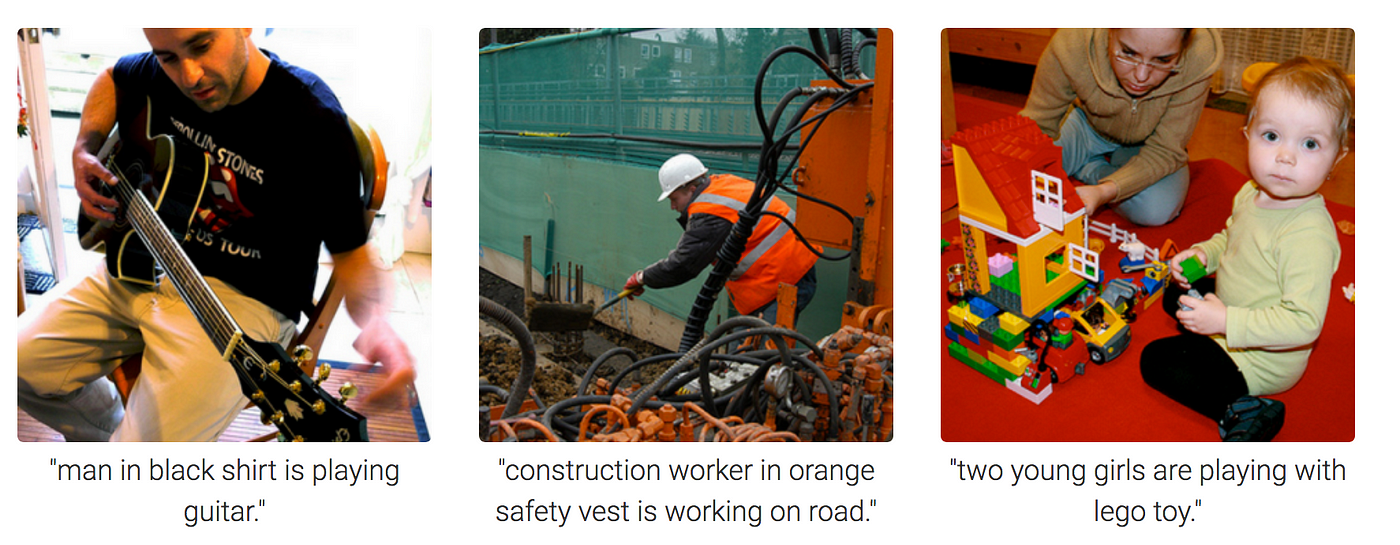
\includegraphics[scale=0.2]{img/image_captioning.png}
      \caption{Image captioning on various image prompts. } 
      \label{fig:image_captioning}
    \end{figure}

 
\section{Energy Models} 

  Note from our machine learning notes that for unsupervised tasks, we have estimated the density of complex distributions by factoring them in \textit{graphical models}, e.g. Bayesian networks or Markov random fields. We will extend this into deep learning architectures.\footnote{This is \textit{not} to be confused with graph neural networks (GNNs), which are designed for tasks whose inputs are graphs.} If you are not familiar, you should probably go over graphical models in my ML notes before reading further. 

  Note that many of the theories behind energy models are very old (from the 1980s) and established. All of them essentially rely on the fact that we can model a probability density as 
  \begin{equation}
    p(x) = \frac{e^{-f(x)}}{Z}
  \end{equation}
  for some function $f: \mathbb{R}^n \rightarrow \mathbb{R}$, and $Z$ is what we call the \textbf{partition function}. We have seen from the Hammersley-Clifford theorem in my machine learning notes that we can model a joint probability distribution on an undirected graph with the product of potential functions on the max cliques.\footnote{But finding max cliques is NP-hard?} Therefore, we will take advantage of this in the specific instance of MRFs that are \textit{bipartite graphs}, i.e. a non-feedforward (since its cyclic) 2-layer neural network. We will talk about RBMs, deep belief networks, and hopfield networks. Diffusion models, which can also be considered an energy model, will be talked separately. 

\subsection{Boltzmann Machines} 

  Consider the graph $x_1, \ldots, x_D$ which represents a random vector $x$ for which we would like to model the probability distribution of. 
  \begin{center}
    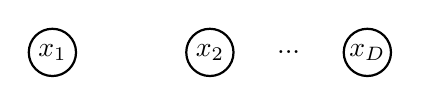
\begin{tikzpicture}
      \node (x1) at (0,0) {$x_1$};
      \node (x2) at (2,0) {$x_2$};
      \node (xD) at (4,0) {$x_D$};

      \node at (3,0) {...};
      \draw[thick] (x1) circle (0.3);
      \draw[thick] (x2) circle (0.3);
      \draw[thick] (xD) circle (0.3);
    \end{tikzpicture}
  \end{center}
  What we can do is model the dependencies between these random elements with linear parameters $W$ and $b$, which essentially gives us a Markov Random Field. Let's consider when $x_i$'s are all Bernoulli, so $x \in \{0, 1\}^D$, which are known as \textit{Ising models} in statistical mechanics. By Hammersley-Clifford, we don't even need to specify the individual functions over the maximal cliques, and rather we can just specify the energy function $E(x)$ of the Boltzmann distribution that the MRF encodes. We parameterize $\theta = \{W, b\}$. 

  \begin{example}[Bernoulli Pairwise Markov Random Fields]
    We define it to capture the interactions between Bernoulli random variables $x_i$ up to order $2$. 
    \begin{equation}
      p_{\theta} (x) = \frac{1}{Z} \exp( E(x)) = \frac{1}{Z} \exp \bigg( \sum_{i j \in E} x_i x_j W_{ij} + \sum_{i \in V} x_i b_i \bigg) = \frac{1}{Z} \exp \big( x^T W x + b^T x \big)
    \end{equation}
    Now let's check its conditional distribution. Let $x_{-k}$ denote the joint distribution of all random variables minus $x_k$.  
    \begin{align}
      p(x_k = 1 \mid x_{-k}) & = \frac{p(x_k = 1, x_{-k})}{p(x_{-k})} \\
                             & = \frac{p(x_k = 1, x_{-k})}{p(x_k = 0, x_{-k}) + p(x_k = 1, x_{-k})} \\
                             & = \frac{\exp \Big( \sum_{k j \in E} x_j W_{kj} + x_k b_k \Big)}{\exp(0) + \exp \Big(\sum_{k j \in E} x_j W_{kj} + x_k b_k \Big)} \\
                             & = \sigma \bigg\{ - b_k x_k - \sum_{k j \in E} x_j W_{k j} \bigg\} 
    \end{align}
    where the penultimate step comes from evaluating 
    \begin{align} 
      p(x_k = 1, x_{-k}) & = \frac{1}{Z(\theta)} \exp \bigg( \sum_{ij \in E, k \neq i, j} x_i x_j W_{ij} + \sum_{i j \in E, k = i, j} x_i x_j W_{ij} + \sum_{i \in V, i \neq k} x_i b_i + x_k b_k \bigg) \\
                         & =\frac{1}{Z(\theta)} \exp \bigg( \sum_{ij \in E, k \neq i, j} x_i x_j W_{ij} + \sum_{k j \in E} x_j W_{kj} + \sum_{i \in V, i \neq k} x_i b_i + b_k \bigg)  \\ 
      p(x_k = 0, x_{-k}) & = \frac{1}{Z(\theta)} \exp \bigg( \sum_{ij \in E, k \neq i, j} x_i x_j W_{ij} + \sum_{i \in V, i \neq k} x_i b_i\bigg)  
    \end{align}
    and canceling out like terms in the numerator and denominator. This tells us that MRFs are related to logistic function.  
  \end{example}

  \begin{example}[Gaussian Markov Random Fields] 
    If we assume that $p_{\theta} (x)$ follows a multivariate Gaussian distribution, we have 
    \begin{equation}
      p(x \mid \mu, \Sigma) = \frac{1}{Z} \exp \bigg( -\frac{1}{2} (x - \mu)^T \Sigma^{-1} (x - \mu) \bigg)
    \end{equation}
    Since the Gaussian distribution represents at most second-order relationships, it automatically encodes a pairwise MRF. Therefore, we can rewrite 
    \begin{equation}
      p(x) = \frac{1}{Z} \exp \bigg( -\frac{1}{2} x^T Jx + g^T x \bigg)
    \end{equation}
    where $J = \Sigma^{-1}$ and $\mu = J^{-1} g$. 
  \end{example}

  However, this is still quite a limited model. For one, due to the linearity of the weight matrix, it always turns out that the probability of $x_k = 1$ is always given by a linear model (logistic regression) from the values of the other units. This family of distributions parameterized by $\theta = \{W, b\}$ may not be broad enough to capture the true $p(x)$. Therefore, we can add latent variables that can act similarly to hidden units in a MLP and model higher-order interactions among the visible units. Just as the addition of hidden units to convert logistic regression into MLP results in the MLP being a universal approximator of functions, a Boltzmann machine with hidden units is not longer limited to modeling linear relationships between variables. Instead, the Boltzmann machine becomes a universal approximator of probability mass functions over discrete random variables. 

  \begin{definition}[Boltzmann Machine]
    The original \textbf{Boltzmann machine} has the energy function 
    \begin{equation}
      E(v, h) = - v^T R v - v^T W h - h^T S h - b^T v - c^T h
    \end{equation}
    It can represent the undirected graph that has connections within the $x$, within the $h$, and between the $x$ and $h$.

    \begin{figure}[H]
      \centering 
      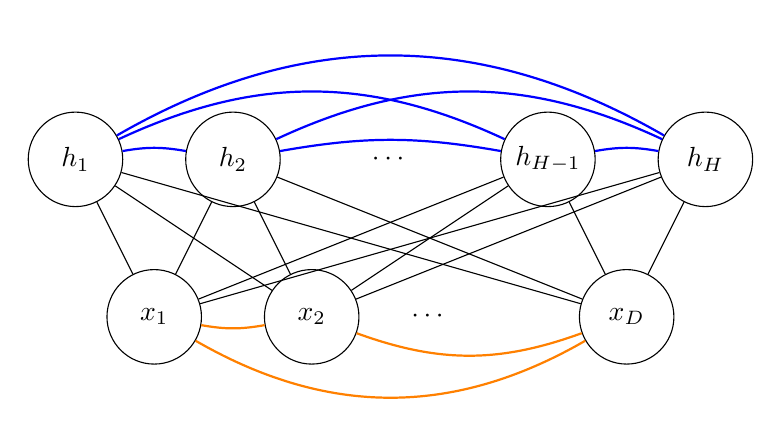
\begin{tikzpicture}[
        node/.style={circle, draw, minimum size=1.2cm},
        every edge/.style={draw, -}
      ]
        % Create h nodes (top layer)
        \node[node] (h1) at (0,2) {$h_1$};
        \node[node] (h2) at (2,2) {$h_2$};
        \node at (4,2) {$\cdots$};
        \node[node] (hm1) at (6,2) {$h_{H-1}$};
        \node[node] (hH) at (8,2) {$h_H$};

        % Create x nodes (bottom layer)
        \node[node] (x1) at (1,0) {$x_1$};
        \node[node] (x2) at (3,0) {$x_2$};
        \node at (4.5,0) {$\cdots$};
        \node[node] (xD) at (7,0) {$x_D$};

        % Draw connections between layers
        \foreach \i in {1,2,m1,H} {
            \foreach \j in {1,2,D} {
              \draw (h\i) -- (x\j);
            }
        }

        % Draw the blue arc on top
        \draw[blue, thick] (h1) to[bend left=30] node[above] {} (hH);
        \draw[blue, thick] (h1) to[bend left=10] node[above] {} (h2);
        \draw[blue, thick] (h1) to[bend left=25] node[above] {} (hm1);
        \draw[blue, thick] (hm1) to[bend left=10] node[above] {} (hH);
        \draw[blue, thick] (h2) to[bend left=10] node[above] {} (hm1);
        \draw[blue, thick] (h2) to[bend left=25] node[above] {} (hH);

        % Draw the orange arc on bottom
        \draw[orange, thick] (x1) to[bend right=30] node[below] {} (xD);
        \draw[orange, thick] (x1) to[bend right=10] node[below] {} (x2);
        \draw[orange, thick] (x2) to[bend right=20] node[below] {} (xD);
      \end{tikzpicture}
      \caption{2-layer undirected graph representing a Boltzmann machine. } 
      \label{fig:boltzmann}
    \end{figure}
  \end{definition} 

  Therefore, by adding latent variables and connecting everything together, this gives us a very flexible model that can capture a lot of distributions.  

\subsection{Restricted Boltzmann Machines} 

  Unfortunately, there are problems with training this, and so the restricted Boltzmann machine allowed for efficient training. Therefore, we will limit ourselves to \textbf{pairwise MRFs}, which only capture dependencies between cliques of maximum size $2$. We usually write $x$ as the observed and $z$ as the latent, but in the literature $v$ and $h$ are used, respectively. Now, if we put a restriction saying that there cannot be any intra-connections in the $x$ and $h$, then we get the \textit{restricted Boltzmann machine}, which has a slightly more resticted form of the energy function than the general BM. 

  \begin{definition}[Restricted Boltzmann Machine] 
    The \textbf{restricted Boltzmann machine} has the energy function 
    \begin{equation}
      E(v, h) = - v^T W h - b^T v - c^T h
    \end{equation}
    with connections only allowed between $x_i$'s and $h_j$'s, known as a \textbf{bipartite graph}, implying that the maximum clique length is $2$. This model allows the elements of $x$ to be dependent, but this architecture allows for \textit{conditional independence}, and not just for $x$ given $h$, but also $h$ given $x$. Therefore, we already have the extremely nice property that 
    \begin{align} 
      p(x \mid h) & = \prod_{k=1}^{D} p(x_k \mid h) \\
      p(h \mid x) & = \prod_{j=1}^F p(h_j \mid x) 
    \end{align}

    \begin{figure}[H]
      \centering 
      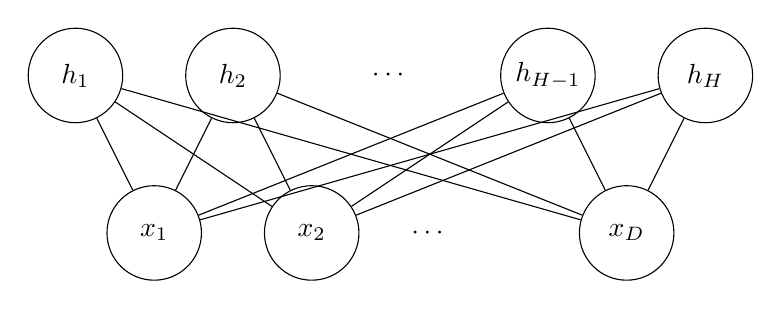
\begin{tikzpicture}[
        node/.style={circle, draw, minimum size=1.2cm},
        every edge/.style={draw, -}
      ]
        % Create h nodes (top layer)
        \node[node] (h1) at (0,2) {$h_1$};
        \node[node] (h2) at (2,2) {$h_2$};
        \node at (4,2) {$\cdots$};
        \node[node] (hm1) at (6,2) {$h_{H-1}$};
        \node[node] (hH) at (8,2) {$h_H$};

        % Create x nodes (bottom layer)
        \node[node] (x1) at (1,0) {$x_1$};
        \node[node] (x2) at (3,0) {$x_2$};
        \node at (4.5,0) {$\cdots$};
        \node[node] (xD) at (7,0) {$x_D$};

        % Draw connections between layers
        \foreach \i in {1,2,m1,H} {
            \foreach \j in {1,2,D} {
              \draw (h\i) -- (x\j);
            }
        }
      \end{tikzpicture}
      \caption{2-layer undirected graph representing a restricted Boltzmann machine. Note that the intra-connections (blue and orange) are gone. } 
      \label{fig:rbm}
    \end{figure}
  \end{definition}

  Note that this form of the probability $E(x)$ is equivalent to the product of max-cliques, which are of size 2 in this case. 
  \begin{align}
    p(v, h) & = \exp(-E(v, h)) / Z \\ 
            & = \exp(v^T W h + b^T v + c^T h) / Z \\
            & = \exp(v^T W h) \exp(b^T v) \exp (c^T h) / Z  \\
            & = \frac{1}{Z} \prod_j \prod_k \exp(W_{jk} h_j v_k) \, \prod_k \exp(c_k v_k) \, \prod_j \exp(b_j h_j)
  \end{align}
  Therefore, we can think of the $\exp(h^T W x)$ as encoding the cliques of length $2$ and the others as cliques of length $1$. The fact that we can calculate $p(h \mid x)$ means that inferring the distribution over the hidden variables is easy. 

  \subsubsection{Contrastive Divergence}

    Now that we've done this, we can finally get to training the model. Now, essentially this is density estimation problem given dataset $\mathcal{D} = \{x^{(t)}\}$ of iid random variables, we want to maximize the likelihood of $p_{\theta}$, which is really just equivalent to optimizing $E_{\theta}$. So, let's take the average negative log-likelihood and take the derivative of it
    \begin{equation}
      \frac{\partial}{\partial \theta} \frac{1}{T} \sum_t - \log p_{\theta} (x^{(t)})
    \end{equation}
    There's a lot of computation to do here, so let's focus on one sample $x^{(t)}$ and claim that the gradient ultimately ends up as the following. 

    \begin{theorem}[Decomposition of Derivative]
      The derivative of the log-likelihood decomposes into the following terms. 
      \begin{align} 
        \frac{\partial}{\partial \theta} - \log p(x^{(t)}) & = \sum_{h}  p(h \mid x^{(t)}) \, \frac{ \partial E(x^{(t)}, h)}{\partial \theta} - \sum_{x, h} p(x, h) \, \frac{\partial E(x, h)}{\partial \theta} \\
                                                           & = \underbrace{\mathbb{E}_{h} \bigg[ \frac{\partial E( x^{(t)}, h)}{\partial \theta} \; \bigg| \; x^{(t)} \bigg]}_{\text{positive phase}} - \underbrace{\mathbb{E}_{x, h} \bigg[ \frac{\partial E(x, h)}{\partial \theta} \bigg]}_{\text{negative phase}}
      \end{align}
      which reduces to 
      \begin{equation}
        -\nabla_\theta \ln{p(x)} = \begin{cases}
          - \nabla_W \ln{p(x)} & = \sum_h p(h \mid x) h x^T - \sum_{x, h} p(x, h) h x^T \\
          - \nabla_b \ln{p(x)} & =  \sum_h p(h \mid x) h - \sum_{x, h} p(x, h) h \\
          - \nabla_c \ln{p(x)} & =  \sum_h p(h \mid x) x - \sum_{x, h} p(x, h) x
        \end{cases}
      \end{equation}
    \end{theorem}
    \begin{proof}
      From the energy model form, we can see that $Z = \sum_{x, h} \exp(-E(x, h))$. Therefore, 
      \begin{align}
        \ln(Z) & = \ln \bigg( \sum_{x, h} \exp(-E(x, h)) \bigg) \\ 
        \frac{\partial}{\partial \theta} \ln(Z) & = \frac{1}{Z} \sum_{x, h} \exp(-E(x, h)) \cdot -1 \cdot \frac{\partial}{\partial \theta} E(x, h) \\
               & = -\frac{1}{Z} \sum_{x, h} \exp(-E(x, h)) \cdot \frac{\partial}{\partial \theta} E(x, h) \\
               & = -\frac{1}{Z} \sum_{x, h} Z \cdot p(x, h) \cdot \frac{\partial}{\partial \theta} E(x, h) \\
               & = - \sum_{x, h} p(x, h) \frac{\partial E(x, h)}{\partial \theta}
      \end{align}
      We have by definition 
      \begin{equation} 
        -\ln p(x) = - \ln \bigg\{ \sum_{h} \exp \big( -E(x, h) \big) \bigg\} + \ln(Z)
      \end{equation}
      and so when taking the derivative, the second term is solved from above and the first term, we apply the chain rule to get 
      \begin{align} 
        -\frac{\partial}{\partial \theta} \ln p(x) & = \frac{\sum_{h} \exp \big( -E(x, h) \big) \, \frac{\partial E(x, h)}{\partial \theta} / Z}{\sum_{h} \exp \big( -E (x, h) \big) / Z} + \frac{\partial \ln(Z)}{\partial \theta} \\
                                                                         & = \frac{\sum_{h} p(x, h) \, \frac{\partial E(x, h)}{\partial \theta}}{p(x)} + \frac{\partial \ln(Z)}{\partial \theta} \\
                                                                         & = \sum_{h} p(h \mid x) \, \frac{\partial E(x, h)}{\partial \theta} - \sum_{x, h} p(x, h) \, \frac{\partial E(x, h)}{\partial \theta} 
      \end{align} 
      We can use the closed form of $E$ to then compute its partials. 
      \begin{align}
        \bigg( \frac{\partial E(x, h)}{\partial W} \bigg)_{ij} & = \frac{\partial E(x, h)}{\partial W_{ij}} = \frac{\partial}{\partial W_{ij}} \bigg\{ - \sum_{i,j} W_{ij} h_i x_j - \sum_j c_j x_j - \sum_i b_i h_i \bigg\} = h_i x_j \\
        \bigg( \frac{\partial E(x, h)}{\partial b} \bigg)_i & = \frac{\partial E(x, h)}{\partial b_i} = h_i  \\
        \bigg( \frac{\partial E(x, h)}{\partial c} \bigg)_j & = \frac{\partial E(x, h)}{\partial c_j} = x_j 
      \end{align}  
      which in matrix form is 
      \begin{align}
        \nabla_{\theta} E(x, h) = \{ \nabla_W E(x, h), \nabla_b E(x, h), \nabla_c E(x, h) \} = \{ h x^T, h, x \}
      \end{align}
      The conditional probability can be factorized out given $x$ and computed easily by conditional independence. 
      \begin{equation}
        p(h \mid x) = \prod_j p(h_j \mid x)
      \end{equation}
      and so given that we have computed this for all $h$, we can write our gradient as 
      \begin{equation}
        -\nabla_\theta \ln{p(x)} = \begin{cases}
          - \nabla_W \ln{p(x)} & = \sum_h p(h \mid x) h x^T - \sum_{x, h} p(x, h) h x^T \\
          - \nabla_b \ln{p(x)} & =  \sum_h p(h \mid x) h - \sum_{x, h} p(x, h) h \\
          - \nabla_c \ln{p(x)} & =  \sum_h p(h \mid x) x - \sum_{x, h} p(x, h) x
        \end{cases}
      \end{equation}
    \end{proof} 

    Therefore, we can easily compute the left summation in the gradient form, but the right summation requires us to compute $p(x, h)$ as a general joint distribution, which is intractable. So we just approximate this with a Monte Carlo estimator, specifically Gibbs sampling. This method is known as \textit{contrastive divergence}. 

    \begin{algo}[Contrastive Divergence] 
      The general idea is to replace by the expectation by a point estimate at $\Tilde{x}$, which we can obtain by sampling the conditions over and over through Gibbs. Since we know $p(x\mid h)$ and $p(h \mid x)$ easily, we can start sampling the chain for some predetermined $K$ steps (actually $2K$ since we are sampling the $x$ and $h$ back and forth), and whatever $\Tilde{x}, \Tilde{h}$ you sample at the end is your estimate. You then use this to approximate the negative phase 
      \begin{equation}
        \mathbb{E}_{x, h} \bigg[ \frac{\partial E(x, h)}{\partial \theta} \bigg] \approx \frac{\partial}{\partial \theta} E(\Tilde{x}, \Tilde{h})
      \end{equation}
      Here are the steps. 
      \begin{enumerate}
        \item Initialize $x^0 = x$ and sample $h^0$ from $p(h \mid x^0)$. 
        \item For $k = 1, \ldots, K$, 
        \begin{enumerate}
          \item Sample $x^k$ from $p(x \mid h^{k-1})$. 
          \item Sample $h^k$ from $p(h \mid x^k)$. 
        \end{enumerate}
        \item Once you get $\Tilde{x} = x^K$,\footnote{Note that we do not use $\Tilde{h} = h^K$.} use this to approximate 
        \begin{align}
          - \nabla_W \ln{p(x)} & = \sum_h p(h \mid x) h x^T - \sum_{x, h} p(x, h) h x^T && \approx \sum_h p(h \mid x) h x^T - \sum_h p(h \mid \Tilde{x}) h \Tilde{x}^T \\
          - \nabla_b \ln{p(x)} & =  \sum_h p(h \mid x) h - \sum_{x, h} p(x, h) h && \approx \sum_h p(h \mid x) h - \sum_h p(h \mid \Tilde{x}) h \\
          - \nabla_c \ln{p(x)} & =  \sum_h p(h \mid x) x - \sum_{x, h} p(x, h) x && \approx \sum_h p(h \mid x) x - \sum_h p(h \mid \Tilde{x}) \Tilde{x}
        \end{align}
      \end{enumerate}

      We can tweak this procedure, such as \textbf{persistent CD}, where instead of initializing the chain to $x^{(t)}$, we can initialize the chain to the negative sample of the last iteration. 

      \begin{figure}[H]
        \centering 
        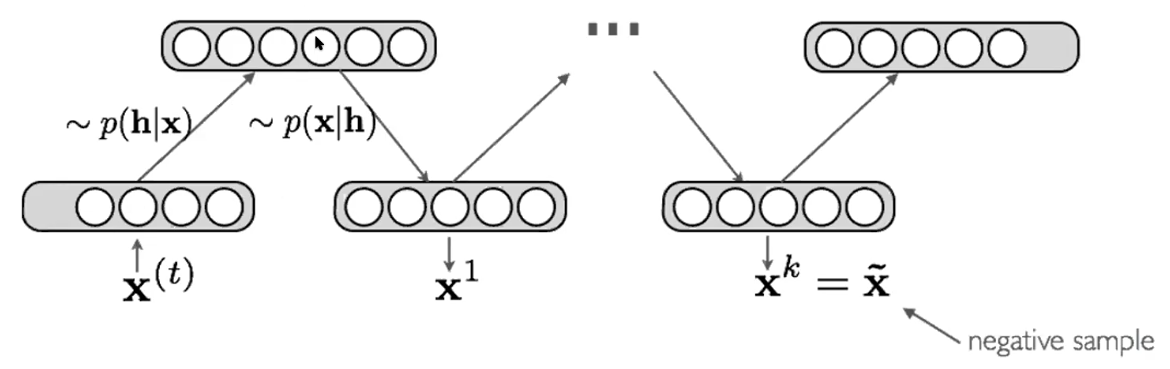
\includegraphics[scale=0.4]{img/07_Boltzmann/contrastive_divergence.png}
        \caption{In general, the bigger $k$ is, the less biased the estimate of the gradient will be, and in practice $k=1$ works well for learning good features. The reason this is called contrastive divergence is that in the gradient update step, we have a positive sample and a negative sample that both approximates the expected gradient, which contrasts to each other. }
        \label{fig:contrastive_divergence}
      \end{figure}
      Therefore, contrastive divergence with $k$ iterations gives us the \textbf{CD-k algorithm}. 
    \end{algo}

    \begin{algo}[Fitting]
      Therefore, for updating $\theta$, we get the following 
      \begin{align} 
        W & = W - \alpha \big( \nabla_{W}(- \log p(x^{(t)})) \big) \\
                   & = W - \alpha \big( \mathbb{E}_{h} [ \nabla_{W} E(x^{(t)}, h) \mid x^{(t)} ] - \mathbb{E}_{x, h} [\nabla_{W} E(x, h) ]\big) \\
                   & = W - \alpha \big( \mathbb{E}_{h} [ \nabla_{W} E(x^{(t)}, h) \mid x^{(t)} ] - \mathbb{E}_{h} [\nabla_{W} E(\bar{x}, h) \mid \bar{x} ]\big) \\
                   & = W + \alpha \big( h(x^{(t)}) (x^{(t)})^T               - h(\bar{x}) \bar{x}^T \big)
      \end{align}
      and doing this over all three parameters leads to 
      \begin{align} 
        W & \leftarrow W + \alpha \big( h (x^{(t)}) (x^{(t)})^T - h(\bar{x}) \bar{x}^T \big) \\
        b & \leftarrow b + \alpha \big( h(x^{(t)}) - h(\bar{x}) \big) \\
        c & = \leftarrow c + \alpha \big( x^{(t)} - \hat{x} \big) 
      \end{align}
    \end{algo} 

    \begin{example}[Collaborative Filtering]
      Netflix dataset. 
    \end{example}

  \subsubsection{Inference with Bernoulli-Bernoulli RBMs}

    We have talked about RBMs of a general form, but the standard is that the hidden units are almost always Bernoulli, while the visible ones are either Bernoulli or Gaussian. Let's talk about when $x, h$ are both Bernoulli, which allows us to simplify the general form of training. 

    \begin{definition}[Bernoulli-Bernoulli RBM]
      For now, let us assume that we are trying to estimate the distribution of a Bernoulli random vector $x \in \{0, 1\}^D$ with Bernoulli latent variables $h \in \{0, 1\}^F$. Then, the energy of the joint configuration is  
      \begin{equation}
        E(v, h; \theta) = - \sum_{ij} W_{ij} v_i h_j - \sum_i b_i v_i - \sum_j a_j h_j = - v^T W h - b^T v - a^T h
      \end{equation}
      where $\theta = \{W, a, b\}$ are the model parameters. 
    \end{definition}

    Let's get some calculations out of the way. 

    \begin{lemma}[Conditional Distributions] 
      For the Bernoulli RBM, we have 
      \begin{align} 
        p(h_j = 1 \mid x) & = \sigma ( b_j + W_{j,:} x) \\
        p(x_k = 1 \mid h) & = \sigma ( c_k + h^T W_{:, k})
      \end{align}
    \end{lemma}
    \begin{proof}
      Just use the definition of conditional probability and substitute the result below in the denominator. The terms will cancel out. 
    \end{proof}

    \begin{lemma}[Free Energy] 
      For the Bernoulli RBM, we want to compute the marginal $p(x)$ as
      \begin{align*} 
      p(x) & = \frac{\exp(-F(x))}{Z} \\
                    & = \frac{1}{Z} \exp \bigg( c^T x + \sum_{j=1}^H \log \big( 1 + \exp (b_j + W_{j, :} x) \big) \bigg) \\
                    & = \frac{1}{Z} \exp \bigg( c^T x + \sum_{j=1}^H \mathrm{softplus}(b_j + W_{j, :} x ) \bigg)
      \end{align*}
      where $F$ is called the \textbf{free energy} and the softplus is defined. 
      \begin{equation}
        \text{softplus}(x) = \ln(1 + e^x)
      \end{equation}
      Therefore, $p(x)$ is calculated by taking the product of these terms, which is why it's known as a \textbf{product of experts model}. 

      \begin{figure}[H]
        \centering 
        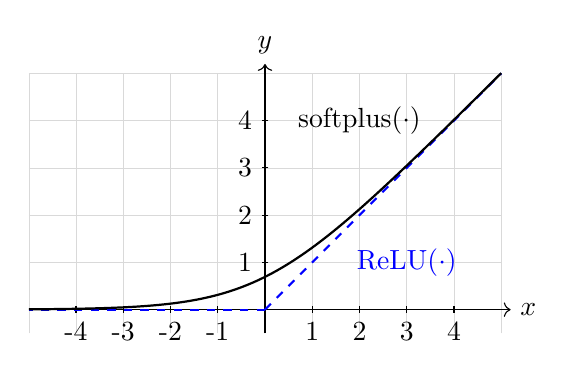
\begin{tikzpicture}[
          scale=0.6,
          declare function={
              softplus(\x) = ln(1 + exp(\x));
          }
        ]
          % Grid and axes
          \draw[very thin,gray!30] (-5,-0.5) grid (5,5);
          \draw[->] (-5,0) -- (5.2,0) node[right] {$x$};
          \draw[->] (0,-0.5) -- (0,5.2) node[above] {$y$};

          % Tick marks
          \foreach \x in {-4,-3,-2,-1,1,2,3,4} {
              \draw (\x,2pt) -- (\x,-2pt) node[below] {\x};
          }
          \foreach \y in {1,2,3,4} {
              \draw (2pt,\y) -- (-2pt,\y) node[left] {\y};
          }

          % Function label
          \node at (2,4) {softplus($\cdot$)};
          \node[blue] at (3,1) {ReLU($\cdot$)};

          % Dashed line (identity function after x>0)
          \draw[thick, blue, dashed] (0,0) -- (5,5);
          \draw[thick, blue, dashed] (0,0) -- (-5,0);

          % Softplus function
          \draw[thick] plot[domain=-5:5, samples=100] (\x,{softplus(\x)});
        \end{tikzpicture}
        \caption{A graph of the softplus activation function, with the dotted ReLU.} 
        \label{fig:softplus}
      \end{figure}
    \end{lemma}
    \begin{proof}
      We have 
      \begin{align} 
        p(x) & = \sum_{h \in \{0, 1\}^H} \exp \big( h W x + c^T x + b^T h\big) /Z \\
                      & = \exp (c^T x) \sum_{h_1 = 0, 1} \ldots \sum_{h_H = 0, 1} \exp \bigg( \sum_j h_j W_{j, :} x + b_j h_j \bigg) / Z \\
                      & = \exp (c^T x) \bigg( \sum_{h_1 = 0, 1} \exp (h_1 W_{1, :} x + b_1 h_1 ) \bigg) \ldots \bigg( \sum_{h_H = 0, 1} \exp (h_H W_{H, :} x + b_H h_H) \bigg) / Z \\
                      & = \exp (c^T x) \big( 1 + \exp (b_1 + W_{1, :} x) \big) \ldots \big( 1 + \exp (b_H + W_{H, :} x)\big) / Z \\
                      & = \exp (c^T x) \exp\big\{ \log \big( 1 + \exp (b_1 + W_{1, :} x) \big) \big\} \ldots \exp \big\{ \log \big( 1 + \exp (b_H + W_{H, :} x) \big) \big\} / Z \\
                      & = \frac{1}{Z} \exp \bigg( c^T x + \sum_{j=1}^H \log \big( 1 + \exp (b_j + W_{j, :} x) \big) \bigg) 
      \end{align} 
    \end{proof}

    When training, we can use the closed form to simplify our calculations. 
    \begin{equation}
      \frac{\partial E(x, h)}{\partial W_{j k}} = \frac{\partial}{\partial W_{j k}} 
    \end{equation}
    and so 
    \begin{equation}
      \mathbb{E}_{h} \bigg[ \frac{\partial E(x, h)}{\partial W_{j k}} \bigg| x \bigg] = \mathbb{E}_{h} [ -h_j x_k \mid x] = \sum_{h_j = 0, 1} - h_j x_k \, p(h_j \mid x) = - x_k p(h_j = 1 \mid x)
    \end{equation}
    where the final term is a sigmoid. Hence, we have 
    \begin{equation}
      \mathbb{E}_{h} [ \nabla_{W} E(w, h) \mid x] = - h(x) x^T, \text{ where } h(x) \coloneqq \begin{pmatrix} p(h_1 = 1 \mid x) \\ \vdots \\ p(h_H = 1 \mid x) \end{pmatrix} = \sigma(b + W x)
    \end{equation}
    Now we can substitute what we solved into the second expectation, but again this is infeasible to calculate 
    \begin{equation}
      \mathbb{E}_{x, h} \bigg[ \frac{\partial E(x, h)}{\partial\theta}\bigg] = \sum_{x, h} h(x) x^T p(x, h)
    \end{equation}


  \subsubsection{Inference with Gaussian-Bernoulli RBMs}

    Now we can talk about Gaussian Bernoulli RBMs. 

    \begin{definition}[Gaussian-Bernoulli RBM] 
      If we assume that $v$ is a real-valued (unbounded) input that follows a Gaussian distribution (with $h$ still Bernoulli), then we can add a quadratic term to the energy function 
      \begin{equation} 
        E(x, h) = - h^T W x - c^T x - b^T h - \frac{1}{2} x^T x
      \end{equation}
      In this case, $p(x \mid h)$ becomes a Gaussian distribution $N(c + W^T h, I)$. The training process is slightly harder for this, so what we usually do is normalize the training set by subtracting the mean off each input and dividing the input by the training set standard deviation to get  
      \begin{equation} 
        E(v, h; \theta) = \sum_i \frac{(v_i - b_i)^2}{2 \sigma_i^2} - \sum_{ij} W_{ij} h_j \frac{v_i}{\sigma_i} - \sum_j a_j h_j
      \end{equation}
      You should also use a smaller learning rate $\alpha$ compared to Bernoulli RBM. 
    \end{definition} 

    \begin{algo}[Implementation]
      For an implementation with PyTorch, see \href{code/rbm.html}{here}. 
    \end{algo}

\subsection{Deep Belief Network} 

  So far, BMs and RBMs aren't really \textit{deep} since they are shallow 2-layer networks, and I could have placed them in my machine learning notes in graphical models. However, RBMs provided the foundations for deep belief networks, a pivotal moment in deep learning, and thus they are considered part of the deep learning curriculum. 

\subsection{Hopfield Networks}


\section{Variational Autoencoders}

  Variational autoencoders are very good at generating fake data/images. The general construction of VAEs, which bridges graphical models and deep learning, is based on generative probability models and does not really need to be implemented using neural nets. VAEs based on deep learning were proposed in 2013. 

  We start off by stating a fundamental problem with autoencoders. The latent space where the encoded vectors lie may not be contiguous or allow easy interpretation. 

  \begin{figure}[H]
    \centering 
    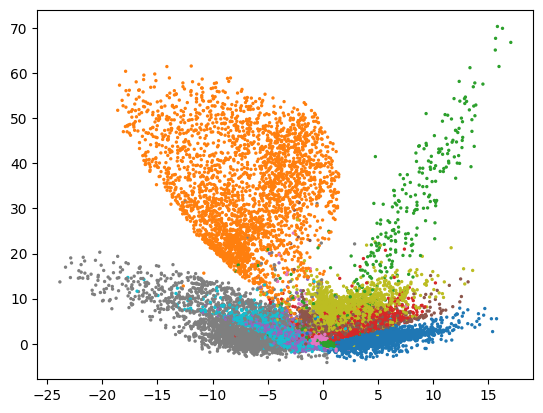
\includegraphics[scale=0.4]{img/08_VAE/mnist_latent.png}
    \caption{Training an autoencoder on MNIST and then visualizing the encodings from a 2D latent space shows the formation of distinct clusters, but there are huge empty spaces where the labeling may be ambiguous and not allow us to interpolate effectively. What if we get an image that happens to land in an empty region in the latent space (e.g. some badly written digit that looks like it's between 1 and 7), how should we interpret it? }
    \label{fig:mnist_latent}
  \end{figure}

  Ideally, we want the encodings to be close to being contiguous while still being distinct. This allows smooth interpolation and enables construction of \textit{new} samples. If the space has discontinuities and you sample a variation from there, the decoder will simply generate an unrealistic output. 
  \begin{figure}[H]
    \centering 
    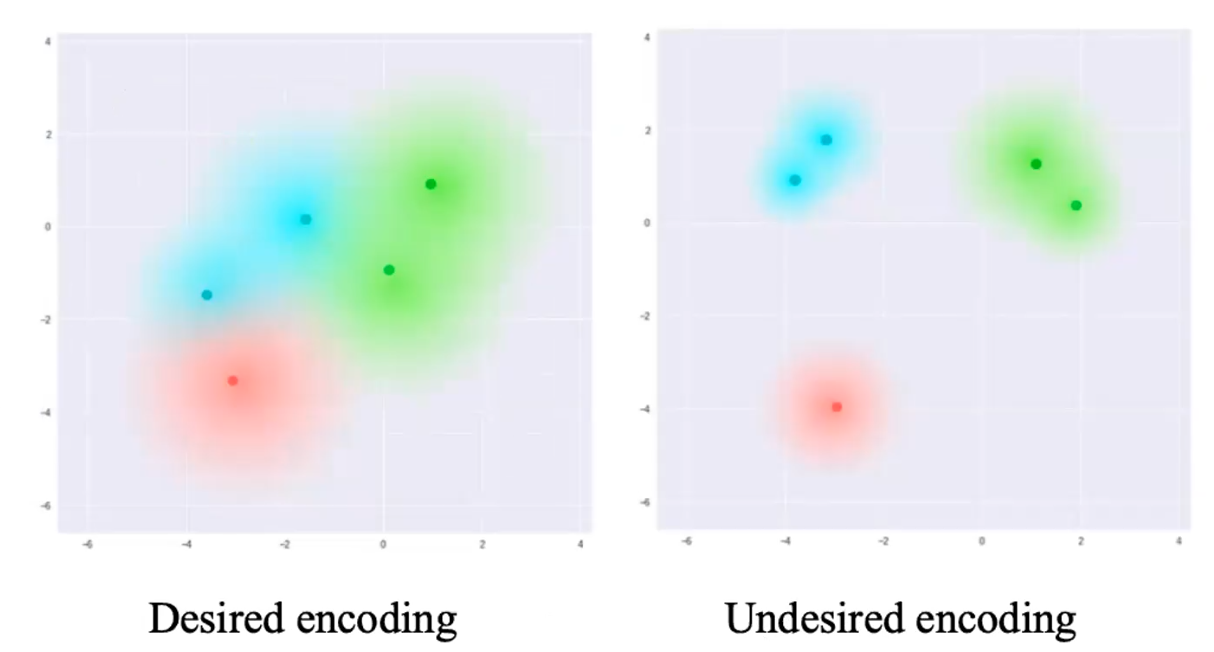
\includegraphics[scale=0.3]{img/08_VAE/contiguous_encoding.png}
    \caption{} 
    \label{fig:contiguous_encoding}
  \end{figure}

  The general idea here is to replace all the ``point-estimates" into distributions in a regular autoencoder. In a way, we have done this already in softmax classification. In a classification neural network, it takes in an input $\mathbf{x}$ and outputs a softmax vector $NN(\mathbf{x}) =(p_1, \ldots, p_K)^T$. This basically means that $NN(\mathbf{x}) = \boldsymbol{\theta}$ parameterizes the conditional distribution (in this case, multinomial) of $\mathbf{y}$ given $\mathbf{x}$. 
  \begin{equation}
    Y \mid X = x \sim \mathrm{Multinomial}(\boldsymbol{\theta} = NN(\mathbf{x}))
  \end{equation}
  This is a much more efficient way to store conditional distributions than a $\dim(X) (K - 1)$ lookup table. 

  \subsection{Deep Latent Variable Models}

    Latent variable models that uses some deep learning architecture is pretty much what DLVMs are. This is essentially what we want to extend. We take a latent model $(\mathbf{x}, \mathbf{z})$ and want to approximate $p(\mathbf{x}, \mathbf{z})$. There are essentially 2 things we're interested in: 
    \begin{enumerate}
        \item \textbf{Generation}: Computing $p(\mathbf{x} \mid \mathbf{z})$. 
        \item \textbf{Inference}: Computing $p(\mathbf{z} \mid \mathbf{x})$. 
    \end{enumerate}
    Given a latent sample $\mathbf{z}$ we want to find the conditional probability distribution of $\mathbf{x}$ given $\mathbf{z}$. We can also assume a simple prior $p(\mathbf{z})$ and calculate 
    \[p(\mathbf{x}, \mathbf{z}) = p(\mathbf{x} \mid \mathbf{z}) \, p(\mathbf{z}) \]
    That is, we generate a latent variable from $p(\mathbf{z})$ and want to use this value to get the parameters of $x \sim p_{\boldsymbol{\theta}} (\mathbf{x} \mid \mathbf{z})$ with some decoder neural network $D_{\boldsymbol{\theta}}$ that parameterizes the distribution. Clearly put, $D_{\boldsymbol{\theta}} (\mathbf{z})$ are the parameters of $\mathbf{X} \mid \mathbf{Z} = \mathbf{z}$. 

    \begin{example}[Bernoulli Random Vector] 
        We would like to approximate a $D$-dimensional Bernoulli vector $\mathbf{x}$ with a latent variable $\mathbf{z} \in \mathbb{R}^K$. We will assume a prior $p(\mathbf{z}) \sim N(\mathbf{0}, \mathbf{I})$, and let us have a neural net $\mathcal{D}_{\boldsymbol{\theta}}$ that parameterizes the random vector $\mathbf{x}$, where $x_i \sim \mathrm{Bernoulli}(p_i)$ for $p_i$. Then,
    \begin{align*}
        p(\mathbf{x} \mid \mathbf{z}) & = \prod_{d=1}^D p(x_d \mid \mathbf{z}) = \prod_{d=1}^D p_d^{x_d} (1 - p_d)^{1 - x_d} = \prod_{d=1}^D [\mathcal{D}_{\boldsymbol{\theta}} (\mathbf{z})]_d^{x_d} \, \big( 1 - [\mathcal{D}_{\boldsymbol{\theta}} (\mathbf{z})]_d\big)^{1 - x_d}
    \end{align*} 
    and we can see that since $\mathbf{p}$ has the flexibility of whatever vector in $[0, 1]^D$ it can be captured by the neural net $\mathcal{D}$. It encompasses a broad family of Bernoulli probability distributions. 
    \end{example}

    From the example above, we can see that we have some method to compute $p(\mathbf{x} \mid \mathbf{z})$. We train a neural net (somehow) and do forward prop on it to generate the correct parameters modeling the distribution of $\mathbf{x}$. However, computing 
    \[p(\mathbf{x}) = \int p(\mathbf{x}, \mathbf{z}) \,d\mathbf{z} = \int p_{\boldsymbol{\theta}} (\mathbf{x} \mid \mathbf{z}) \, p(\mathbf{z}) \,d\mathbf{z} \]
    is computationally intractable (note that in RBMs the conditional independence allowed us to integrate over $\mathbf{z}$ easily). To see why, in the example above, the integral becomes
    \[p(\mathbf{x}) = \sum_{\mathbf{z} \in \{0, 1\}^K} \underbrace{\prod_{d=1}^D [\mathcal{D}_{\boldsymbol{\theta}} (\mathbf{z})]_d^{x_d} \big( 1 - \mathcal{D}_{\boldsymbol{\theta}} (\mathbf{z})]_d \big)^{1 - x_d}}_{\text{complex}} \, p(\mathbf{z}) \, d\mathbf{z}\]
    and integrating over all $\mathbf{z}$'s for more complex spaces is not feasible. Now let's focus on $p(\mathbf{z} | \mathbf{x})$. By Bayes rule, we can calculate 
    \[p(\mathbf{z} \mid \mathbf{x}) = \frac{p(\mathbf{x} \mid \mathbf{z}) p(\mathbf{z})}{p(\mathbf{x})}\]
    Where we have established the intractability of the denominator. The first thing that comes to mind is to just do MCMC since $p(\mathbf{z} \mid \mathbf{x}) \propto p(\mathbf{x} \mid \mathbf{z}) p(\mathbf{z})$, but the forward propagation is too slow to sample efficiently. So, we must use our other trick in the book: \textbf{variational Bayes/inference}. 

    To do this, we construct another family of probability distributions parameterized by $\lambda$: $\{ q_{\lambda} (\mathbf{z} \mid \mathbf{x})\}$, and we want to find a $\lambda$ such that $q_{\lambda} (\mathbf{z} \mid \mathbf{x}) \approx p_{\boldsymbol{\theta}} (\mathbf{z} \mid \mathbf{x})$. Just like the generation model, we can build another neural network $\mathcal{E}_{\phi}$ such that $\lambda = \mathcal{E}_{\phi} (\mathbf{x})$ parameterizes the conditional distribution of $\mathbf{z}$. Essentially we are trying to construct an encoder and a decoder, which can be represented by the diagram below. 
    \begin{center}
        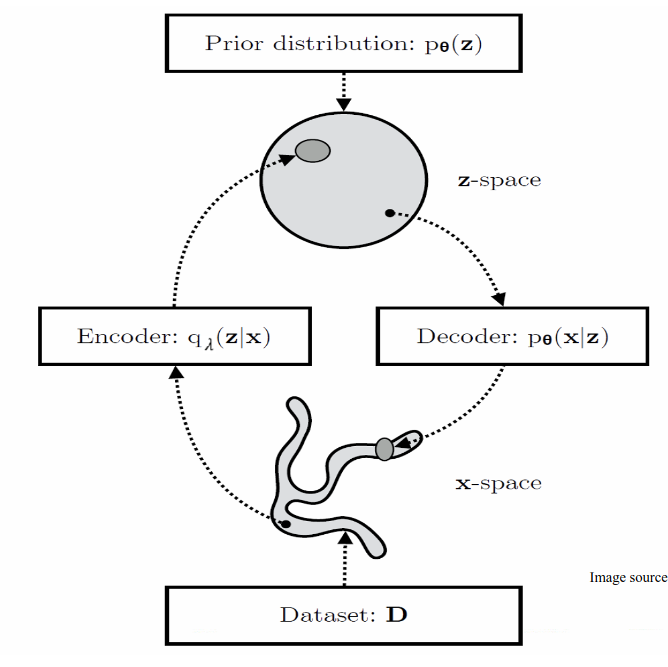
\includegraphics[scale=0.4]{img/08_VAE/VAE_framework.png}
    \end{center}
    If $q_{\lambda} = p_{\boldsymbol{\theta}}$, then the diagram commutes, i.e. $p(\mathbf{z}) p_{\boldsymbol{\theta}}(\mathbf{x} \mid \mathbf{z}) = p(\mathbf{x}) p_{\boldsymbol{\theta}}(\mathbf{z} \mid \mathbf{x}) = p_{\boldsymbol{\theta}} (\mathbf{x}, \mathbf{z})$. 
     
    \begin{example}
        If $\lambda = (\boldsymbol{\mu}, \boldsymbol{\sigma})$, where $\boldsymbol{\sigma}$ is just the vector representing variances of independent Gaussians, then we can use the neural network $\mathcal{E}$ to get 
        \[\lambda = \mathrm{EncoderNN}_{\phi} ( \mathbf{x}) = \mathcal{E}_{\phi} (\mathbf{x})\]
        In the example, $\lambda = (\boldsymbol{\mu}, \log \boldsymbol{\sigma}^2 )$ since we want to allow negative values, and $q_{\lambda} (\mathbf{z} \mid \mathbf{x}) = N(\mathbf{z} \mid \mathcal{E}_{\phi} (\mathbf{x})) = N(\mathbf{z} ; \, \boldsymbol{\mu} , \boldsymbol{\sigma}^2)$. 
    \end{example}

    Now, just like in RBMs and really any density estimation problem, our job is to maximize the log likelihood of the training set: 
    \[\sum_{t} \log p(\mathbf{x}^{(t)})\]

    In order to do this for this problem, we need a little fact to help us: 

    \begin{theorem}
    We have 
    \[KL \big( q_\lambda (\mathbf{z} \mid \mathbf{x}) \mid\mid p_{\boldsymbol{\theta}} (\mathbf{z} \mid \mathbf{x}) \big) = \mathbb{E}_{q_\lambda(\mathbf{z} \mid \mathbf{x})} [ \log q_{\lambda} (\mathbf{z} \mid \mathbf{x})] + \log p_{\boldsymbol{\theta}} (\mathbf{x}) - \mathbb{E}_{q_{\lambda} (\mathbf{z} \mid \mathbf{x})} [\log p_{\boldsymbol{\theta}} (\mathbf{x}, \mathbf{z})] \]
    and hence 
    \[\log p(\mathbf{x}) = KL \big( q_\lambda (\mathbf{z} \mid \mathbf{x}) \mid\mid p_{\boldsymbol{\theta}} (\mathbf{z} \mid \mathbf{x}) \big) + \mathbb{E}_{q_{\lambda} (\mathbf{z} \mid \mathbf{x})} [\log p_{\boldsymbol{\theta}} (\mathbf{x}, \mathbf{z})] - \mathbb{E}_{q_\lambda(\mathbf{z} \mid \mathbf{x})} [ \log q_{\lambda} (\mathbf{z} \mid \mathbf{x})]  \]
    \end{theorem}
    \begin{proof}
    TBD 
    \end{proof}

    So I have to maximize $\log  p(\mathbf{x})$ with what we have derived just now, but the KL divergence part is intractable, since $p_{\boldsymbol{\theta}} (\mathbf{z} \mid \mathbf{x})$ is intractable. That is the entire reason we chose $q_\lambda$! Using the fact that the KL divergence is always greater than or equal to $0$, we can drop the term and set a lower bound on the log likelihoods. This lower bound is called the \textbf{variational lower bound}.  
    \[\sum_{i=1}^N \log p_{\boldsymbol{\theta}} (\mathbf{x}^{(i)}) \geq \sum_{i=1}^N \mathbb{E}_{q_\lambda (\mathbf{z} \mid \mathbf{x}^{(i)})} [ \log p_{\boldsymbol{\theta}} (\mathbf{x}^{(i)}, \mathbf{z})] - \sum_{i=1}^N \mathbb{E}_{q_{\lambda} (\mathbf{z} \mid \mathbf{x}^{(i)})} [ \log q_{\lambda} (\mathbf{z} \mid \mathbf{x}^{(i)}) ] = \mathrm{ELBO}\]
    If we assume that no two data points share their latent variables with each other, then ELBO decomposes into the sum of
    \begin{align*} 
        \mathrm{ELBO} & = \sum_{i=1}^N \mathrm{ELBO}_i \\
                      & = \sum_{i=1}^N  \mathbb{E}_{q_\lambda (\mathbf{z} \mid \mathbf{x}^{(i)})} [\log p_{\boldsymbol{\theta}} (\mathbf{x}^{(i)}, \mathbf{z})] - \sum_{ i=1}^N \mathbb{E}_{q_\lambda (\mathbf{z} \mid \mathbf{x}^{(i)})}[ \log  q_{\lambda} (\mathbf{z} \mid \mathbf{x}^{(i)})] \\
                      & = \underbrace{\mathbb{E}_{q_\lambda (\mathbf{z} \mid \mathbf{x}^{(i)})} [\log p_{\boldsymbol{\theta}} (\mathbf{x}^{(i)} \mid \mathbf{z})]}_{\substack{\text{likelihood term} \\ \text{(reconstruction part)}}}- \underbrace{KL(q_{\lambda} (\mathbf{z} \mid \mathbf{x}^{(i)}) \mid\mid p(\mathbf{z}))}_{\substack{\text{closeness of encoding to } p(\mathbf{z}) \\ \text{(typically Gaussian)}}}
    \end{align*} 
    Typtically, $p(\mathbf{z})$ is chosen to be standard normal. This process is true regardless of it model classes $p_{\boldsymbol{\theta}} (\mathbf{x}^{(i)} \mid \mathbf{z})$ and $q_\lambda (\mathbf{z} \mid \mathbf{x})$ are given by deep neural nets or not. If it is a deep neural net, then it's called a deep latent model. 

    Now to compute gradients, let us denote the ELBO w.r.t. the decoder and encoder paramters as $\mathcal{L}_{\theta, \lambda}(\mathbf{x})$. Then, we can obtain the unbiased gradient w.r.t. $\theta$ as such: 
    \begin{align*} 
        \nabla_\theta \mathcal{L}_{\theta, \lambda} (\mathbf{x}) & = \nabla_\theta \big\{ \mathbb{E}_{q_\lambda (\mathbf{z} \mid \mathbf{x})} [ \log p_\theta (\mathbf{x}, \mathbf{z})] - \mathbb{E}_{q_\lambda (\mathbf{z} \mid \mathbf{x})} [\log q_{\lambda} (\mathbf{z} \mid \mathbf{x})] \} \\
                                                                 & = \mathbb{E}_{q_\lambda (\mathbf{z} \mid \mathbf{x})} \big[ \nabla_\theta \{ \log p_[\theta (\mathbf{x}, \mathbf{z}) - \log q_{\lambda} (\mathbf{z} \mid \mathbf{x}) \}  \big] \\
                                                                 & \approx \nabla_\theta \big\{ \log p_\theta(\mathbf{x}, \mathbf{z}) - \log q_\theta (\mathbf{z} \mid \mathbf{x}) \big\} \\
                                                                 & = \nabla_\theta \log p_\theta (\mathbf{x}, \mathbf{z}) 
    \end{align*}
    where the step with the $\approx$ just indicates that we approximate the expectation with a sample of size $1$ over some minibatch. However, taking the gradient w.r.t. $\lambda$ is more complicated since we cannot put the gradient in the expectation (since we are deriving and integrating w.r.t. $\lambda$).  Fortunately, for continuous RVs, the unbiased estimator of the gradient can be obtained through the \textbf{reparamaterization trick}, which is some change of variable. 

    \subsubsection{Reparameterization Trick} 

  \subsection{Variational Autoencoders} 

    In a VAE, the $q_{\lambda} (\mathbf{z} \mid \mathbf{x})$ is the encoder and the $p_{\boldsymbol{\theta}} (\mathbf{x} \mid \mathbf{z})$ is the decoder. 
    \begin{enumerate} 
        \item \textbf{Encoding Neural Network}: Upon observing $\mathbf{x}$, the neural network $\mathcal{E}$ outputs parameters $\lambda$. 
        \item \textbf{Decoding Neural Network}: Upon observing $\mathbf{z}$, the neural network $\mathcal{D}$ outputs parameters $\boldsymbol{\theta}$. 
    \end{enumerate} 

    We want to optimize $(\boldsymbol{\theta}, \lambda)$. To generate new samples, we just sample from $p(\mathbf{z})$ (usually standard Gaussian) and use the decoder to sample from $\mathbf{x}$.  

    This can be extended to deep layers. 

  \subsection{Conditional VAEs}

  \subsection{Importance Weighted Autoencoders}

 
\section{Generative Adversarial Networks} 

  The year after Kigma published his paper on VAEs, Ian Goodfellow in 2014 published \cite{gans} on \textit{generative adversarial networks}. Unlike the current generative models, which relied on ``fancy'' methods like variational Bayes or contrastive divergence, Goodfellow claimed that we can just do this with vanilla MLPs. The general idea is to approximate the true density $p^\ast (x)$, you are trying to build a function (a neural network) $G_\alpha$ that is a transformation of a simple latent variable, e.g. $Z \sim \mathcal{N}(0, 1)$, such that the pdf of $G_\alpha (Z)$ is similar to $p^\ast (x)$. 

  Remember that for the generative models that we have so far, we were able to \textit{explicitly model} the true pdf. 
  \begin{enumerate}
    \item \textit{Explicit and Analytical}. The simplest types of densities can be analytically written and can be sampled from directly (e.g. Gaussian with inverse CDF, Box-Muller transform, and even GMMs). 

    \item \textit{Explicit and Approximate}. More complicated models such as the RBM and VAE cannot be analytically written, but can still be directly sampled from with probabilities. Boltzmann machines approximate the explicit density as $p_\theta (x) = \frac{1}{Z} e^{-E(x, z)}$ for some quadratic term $-E(x, z)$. VAEs construct another family of posterior distributions $\{q_\lambda\}$ where each $\lambda$ is the output of an encoder neural network $E_\alpha$. Later on, we will see that normalizing flows and autoregressive models also fall in this category. 

    \item \textit{Implicit}. GANs approximate the true pdf through a transformation of random variables and are implicit in the way that you can't estimate the probabilities but you can still sample from them.\footnote{Given $Z \sim \mathcal{N}(0, 1)$ and the sine function $f(z) = \sin(z)$, it's hard to analytically compute the pdf of $X = f(Z)$. However, to sample from this, we can just sample $z$ from $Z$ and then transform it through $f$. }

    \begin{figure}[H]
      \centering 
      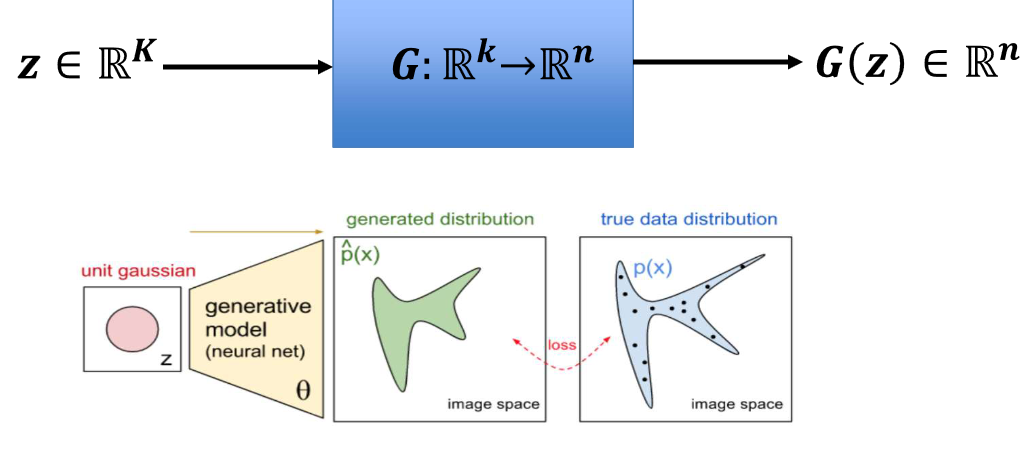
\includegraphics[scale=0.4]{img/09_GAN/implicit_gen_models.png}
      \caption{ You essentially want to take some simple latent distribution and construct a differentiable a \textbf{generator model} that maps it to a more complicated distribution in the observable space. } 
      \label{fig:implicit_gen_models}
    \end{figure}
  \end{enumerate}

  The problem with VAEs is that they tend to generate blurry images, which is the result of optimizing a variational lower bound rather than the true objective. This makes it easy to identify whether a given image is from the true dataset or has been artificially generated. In contrast, GANs generate high-resolution images because we are directly optimizing the true objective. 

  \begin{definition}[Generative Adversarial Networks]
    A \textbf{generative adversarial network (GAN)} is a nonlinear latent-variable model consisting of 
    by optimizing a pair of generator and disciminator neural networks, which play a game where one tries to bea the other. 
    \begin{enumerate} 
      \item A latent random variable $Z$ with pdf $p(z)$. 
      \item The \textbf{generator} tries to generate fake samples to fool the discriminator. We sample from a latent space $\mathbf{z}$ and run that through the neural network to get $\mathbf{x} = \mathcal{G}_{\theta_g} (\mathbf{z})$.i It should be differentiable, but does not have to be invertible.   
      \item The \textbf{discriminator} tries to distinguish between real and fake samples, like a critic which can tell from real from fake. It should also be differentiable, and its output is essentially $0 \leq \mathcal{D}_{\theta_d}(\mathbf{x}) \leq 1$, with a value of $1$ if real, $0$ if fake.  
    \end{enumerate}
    We want to train these two models against each other, and in the end, we throw $\mathcal{D}$ away, since it's only role is to force $\mathcal{G}_{\theta_g}$ to work harder, which leaves us with a really good generative $\mathcal{D}_{\theta_g}$.  
    
    \begin{figure}[H]
      \centering 
      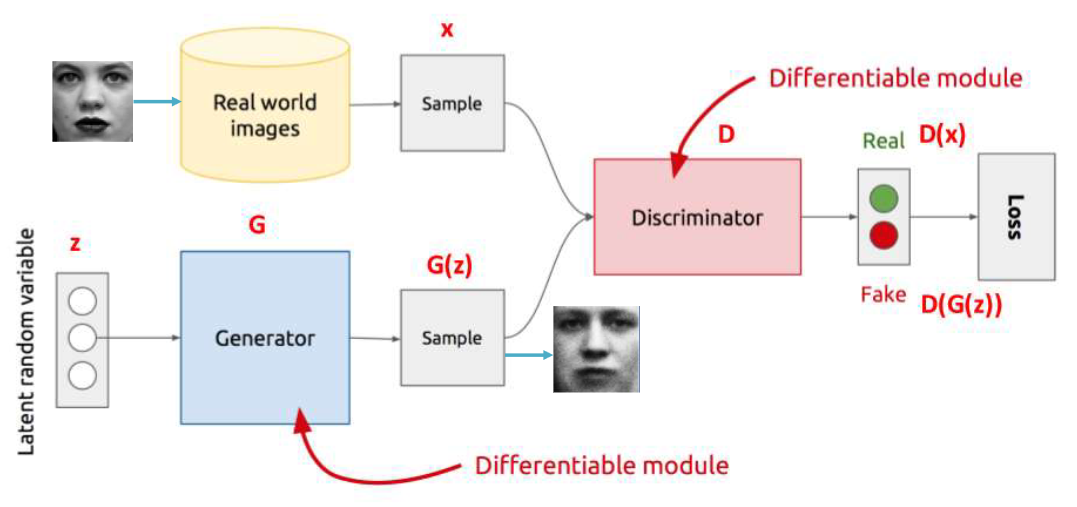
\includegraphics[scale=0.4]{img/09_GAN/general_gan_architecture.png}
      \caption{} 
      \label{fig:gan_arch}
    \end{figure}
  \end{definition}

  \begin{definition}[GAN Loss]
    Now each of these networks will have its own set of parameters which we have to optimize. We want to optimize them by maximizing the likelihood such that the model says ``real" to the samples from the world and ``fake" to the generated samples. This leads to 
    \begin{equation}
      \mathcal{L}(\theta_d, \theta_g) = V(\mathcal{D}, \mathcal{G}) = \underbrace{\mathbb{E}_{x \sim real} \big[ \log \mathcal{D}_{\theta_d}(\mathbf{x}) \big]}_{\substack{\text{log-prob that } \mathcal{D} \text{ correctly} \\ \text{predicts real data as real}}} + \underbrace{\mathbb{E}_{\mathbf{z}} \big[ \log \big( 1 - \mathcal{D}_{\theta_d} ( \mathcal{G}_{\theta_g} (\mathbf{z}))\big)\big]}_{\substack{{log-prob that } \mathcal{D} \text{ correctly} \\ \text{predicts generated data as fake} }}
    \end{equation}
    Therefore, the discrimiator is trying to maximize its reward (to get max value of $0$), and the generator is trying to minimize the disciminator's reward (pulling this log probability down to $-\infty$). This is known as a \textbf{minimax} optimization problem, and we have to find 
    \begin{equation}
      \min_{\theta_g} \max_{\theta_d} V(\mathcal{D}_{\theta_d}, \mathcal{G}_{\theta_g})
    \end{equation}
    which is some saddle point. 
  \end{definition}

  Before we even talk about evaluating the gradients for this, let's prove a result on the properties of such an optimum.   

  \begin{theorem}[Global Optimality] 
    Given the minimax loss above, for a fixed $\mathcal{G}$, the optimal discriminator $\mathcal{D}_G^\ast$ is given by 
    \begin{equation}
      \mathcal{D}_G^\ast (\mathbf{x}) = \frac{p(\mathbf{x} \mid \text{real})}{p(\mathbf{x} \mid \text{real}) + p(\mathbf{x} \mid \text{synthesized})}
    \end{equation}
    Therefore, the global minimum of the training criterion, $\max_{\mathcal{D}} V(\mathcal{D}, \mathcal{G})$ is achieved if and only if 
    \begin{equation}
      p(\mathbf{x} \mid \text{real}) = p(\mathbf{x} \mid \text{synthesized})
    \end{equation}
  \end{theorem}
  \begin{proof} 
    We first have 
    \begin{equation}
      V(\mathcal{D}, \mathcal{G}) = \mathbb{E}_{\mathbf{x} \sim real} \log \mathcal{D}_{\theta_d} (\mathbf{x}) + \mathbb{E}_{\mathbf{z}} \log \big( 1 - \mathcal{D}_{\theta_d} (\mathcal{G}_{\theta_g} (\mathcal{z}))\big) 
    \end{equation}
    Since $\mathcal{G}$ is fixed (i.e. $\theta_g$ is fixed) and acting, we can write the second expectation with respect to the probability measure induced by $\mathcal{G}$.
    \begin{align*} 
      V(\mathcal{D}, \mathcal{G}) & = \mathbb{E}_{\mathbf{x} \sim real} \log \mathcal{D}_{\theta_d} (\mathbf{x}) + \mathbb{E}_{\mathbf{w} \sim \text{fake}} \log \big( 1 - \mathcal{D}_{\theta_d} (\mathbf{w}) \big) \\   
                                      & = \int p(\mathbf{x} \mid \text{real}) \log \mathcal{D}_{\theta_d}(\mathbf{x}) \,d\mathbf{x}+ \int p(\mathbf{x} \mid \text{fake}) \, \log \big( 1 - \mathcal{D}_{\theta_d} (\mathbf{x}) \big) \,d\mathbf{x} 
    \end{align*}
    where the $\mathbf{x}$ in the second integral is a dummy variable. Taking the derivative w.r.t. $\mathbf{x}$ and setting equal to $0$ gives 
    \begin{equation}
      p(\mathbf{x} \mid \text{real}) \frac{1}{\mathcal{D}_{\theta_d} (\mathbf{x})} + p(\mathbf{x} \mid \text{fake}) \cdot \frac{-1}{1 - \mathcal{D}_{\theta_d}(\mathbf{x})} = 0
    \end{equation}
    implies that 
    \begin{equation}
      \mathcal{D}_{\theta_d}( \mathbf{x}) = \frac{p(\mathbf{x} \mid \text{real})}{p(\mathbf{x} \mid \text{real}) + p(\mathbf{x} \mid \text{fake})}
    \end{equation}
  \end{proof} 

  If the discriminator $\mathcal{D}$ is optimal, then the generator is minimizing the \textbf{Jensen-Shannon divergence} between the real and generated (model distributions). However, $\mathcal{D}$ is not optimal in practice since we have limited computational resources, the loss is non-convex, etc. 

  \begin{figure}[H]
    \centering 
    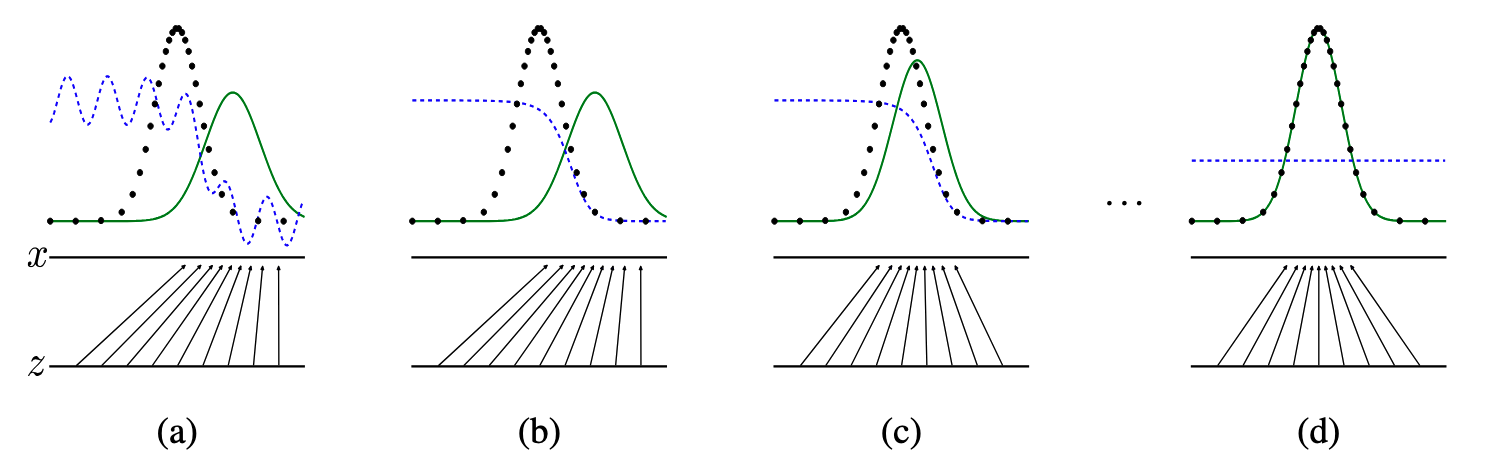
\includegraphics[scale=0.3]{img/equil.png}
    \caption{} 
    \label{fig:nash_equilibrium}
  \end{figure}

  Now we can talk about evaluating the gradients and optimizing it. What is the gradient of such a loss function? This is quite easy since the expectations are over the true data distribution and the known prior $z$, and so we can swap gradients and expectations accordingly. 

  \begin{lemma}[Gradients of GAN Loss]
    
  \end{lemma} 
  \begin{proof}
    
  \end{proof}

  Note that the generator has no effect on the probability of $\mathcal{D}$ correctly identifying real images, so it only focuses on the latter term. 


  \begin{algo}[Alternative Gradient Descent]
    The idea is to train both models simultaneously via SGD using mini-batches consisting of some generated samples and some real-world samples, which is called the \textbf{alternative gradient descent algorithm}. It is usually the case that the generator does better than the disciminator, so we sometimes make $k > 1$ to allow more steps for training. 
    \begin{algorithm}[H]
      \caption{Minibatch stochastic gradient descent training of generative adversarial nets. The number of steps to apply to the discriminator, $k$, is a hyperparameter. We used $k = 1$, the least expensive option, in our experiments.}
      \label{alg:alt_gd}
      \begin{algorithmic}[1] 
        \For{number of training iterations}
            \For{$k$ steps}
                \State Sample minibatch of $m$ noise samples $\{z^{(1)}, \ldots, z^{(m)}\}$ from noise prior $p_g(z)$.
                \State Sample minibatch of $m$ examples $\{x^{(1)}, \ldots, x^{(m)}\}$ from data generating distribution $p_{\text{data}}(x)$.
                \State Update the discriminator by ascending its stochastic gradient:
                \[
                    \nabla_{\theta_d} \frac{1}{m} \sum_{i=1}^m \left[\log D\left(x^{(i)}\right) + \log\left(1-D\left(G\left(z^{(i)}\right)\right)\right)\right].
                \]
            \EndFor
            \State Sample minibatch of $m$ noise samples $\{z^{(1)}, \ldots, z^{(m)}\}$ from noise prior $p_g(z)$.
            \State Update the generator by descending its stochastic gradient:
            \[
                \nabla_{\theta_g} \frac{1}{m} \sum_{i=1}^m \log\left(1-D\left(G\left(z^{(i)}\right)\right)\right).
            \]
        \EndFor
      \end{algorithmic}
    \end{algorithm}
    The gradient-based updates can use any standard gradient-based learning rule. We used momentum in our experiments.
  \end{algo} 

  There is a vanishing gradient problem in GANs. For instance, assume that the model $\mathcal{G}_{\theta_g}$ has very bad parameters, and it generates very bad samples that the disciminator can detect very well. Then, $\mathbb{E}_{\mathbf{z}} \big[ \log \big( 1 - \mathcal{D}_{\theta_d} (\mathcal{G}_{\theta_g}))\big) \big]$ will be very close to $0$, and the generator's cost will be very flat. Therefore, the gradient would die out and the generator can't improve! For example, if $\mathcal{D}$ was just a sigmoid function, then we can approximate the gradient of the expectation with a sample of the gradient, which would die out. 

  \begin{align*} 
    \nabla_{\theta_g} V(\mathcal{D}, \mathcal{G}) & = \nabla_{\theta_g} \mathbb{E}_{z \sim q(\mathbf(\mathbf{z})} \big[ \log \big( 1 - \mathcal{D}(\mathcal{G}(\mathbf{z}))\big) \big] \\
                                                  & \approx \nabla_a \log \big( 1 - \sigma(a)\big) \\
                                                  & = - \frac{\sigma(a) \, \big( 1 - \sigma(a)\big)}{1 - \sigma(a)} = - \sigma(a) = - \mathcal{D}(\mathcal{G}(\mathbf{z})) 
  \end{align*} 

  and so the gradient goes to $0$ if $\mathcal{D}$ is confident, i.e. $\mathcal{D}(\mathcal{G}(\mathbf{z})) \rightarrow 0$. Therefore, we can modify the cost for the generator term by changing the cost to 
  \begin{equation}
    \mathbb{E}_{\mathbf{z}} \log \big( 1 - \mathcal{D}_{\theta_d} ( \mathcal{G}_{\theta_g} (\mathbf{z}))\big)
  \end{equation}
  and trying to minimize it. 


  \begin{theorem}[Convergence]
    
  \end{theorem}

\subsection{Conditional GAN} 

\subsection{CycleGAN}

\subsection{Deep Convolution GAN (DCGAN)} 

  
\section{Normalizing Flows} 

  We have seen many examples of generative models that attempt to produce a probability distribution $p$ that approximates that of the data samples. Some are given by an explicit model (e.g. RBMs) while in others the model is implicit. The key idea for flow-based models\footnote{This has nothing to do with flow graphs and the max-flow-min-cut theorem in graph theory.} is that we want to map simple distributions (e.g. a Gaussian) to complex densities representing the data through an \textit{invertible transformation}. Recall the lemma below from multivariate calculus. 

  \begin{lemma}[Jacobi] 
    Let $X, Z$ be absolutely continuous random variables in $\mathbb{R}^n$. 
    Given that $f: \mathbb{R}^n \rightarrow \mathbb{R}^n$ is invertible and differentiable everywhere, with $X = f(Z), Z = f^{-1} (X)$, we claim 
    \begin{equation}
      p_X (x) = p_Z (f^{-1} (x)) \cdot \big| (D f^{-1}) (x) \big|
    \end{equation} 
    where $|(D f^{-1}) (x)|$ is the determinant of total derivative of $f^{-1}$ at $x$. 
  \end{lemma}
  \begin{proof}
    For $n = 1$, we have 
    \begin{align}
      p_X (x) & = \frac{d}{dx} F_X (x) \\
              & = \frac{d}{dx} F_Z (f^{-1}(x)) \\
              & = p_z (f^{-1} (x)) \cdot \frac{d}{dx} f^{-1} (x)  \\
              & = p_z 
    \end{align}
  \end{proof} 

  Therefore, if we parameterize $f$ with some $\theta$, then the marginal likelihood of $x$ given $\theta$ can be written as 
  \begin{equation}
    p_X (x;\; \theta) = p_Z (f^{-1}_\theta (x)) \cdot | (D f^{-1}_\theta) (x) |
  \end{equation} 
  Therefore, if $X$ is a complex distribution and $Z$ is a simple one (e.g. uniform), we might have hope to efficiently compute $p_X (x)$ for any $x \in \mathbb{R}^n$ if 
  \begin{enumerate}
    \item we can efficiently compute $f^{-1}_\theta (x)$, which allows us to compute $p_Z (f^{-1} (x))$ efficiently since $Z$ is simple. 
    \item we can efficiently compute the Jacobian $Df^{-1} (x)$, and furthermore be able to compute the determinant efficiently.\footnote{Note that computing determinants are approximately $O(n^{2.4})$, which may not be practical. } 
  \end{enumerate} 
  It looks like we have split this enormously hard problem of modeling $X$ with three slightly less difficult problems. However, with some tricks, we may be able to get a simple enough parameterization of $f$ to be able to compute its inverse plus the determinant of the Jacobian. As a first step, what if we add more intermediate functions? Consider the sequence of invertible functions $Z \xrightarrow{f} Y \xrightarrow{g} \rightarrow X$, where $Z$ is a simple distribution that gets transformed to a slightly more complicated distribution $Y$ that then gets transformed to a complex distribution $X$. We can apply the Jacobi theorem above to see $p_Y (y) = p_Z (f^{-1} (y)) \cdot | (Df^{-1})(x)|$, and so we have 
  \begin{align}
    p_X (x) & = p_Y (g^{-1} (x)) \cdot | (D g^{-1}) (x) | \\
            & = p_Z (f^{-1} (g^{-1} (x))) \cdot | (Df^{-1}) (y)| \cdot | (D g^{-1}) (x) | \\ 
            & = p_Z ((g \circ f)^{-1} (x))) \cdot | (Df^{-1}) (y)| \cdot | (D g^{-1}) (x) | 
  \end{align}
  This leads to the following corollary. 

  \begin{corollary}[Jacobi]
    Given a sequence of transformations 
    \begin{equation}
      Z = Z_0 \xrightarrow{f^1} Z_1 \xrightarrow{f^2} \ldots \xrightarrow{f^{M-1}} Z_{M-1} \xrightarrow{f^M} Z_M = X
    \end{equation} 
    where each $f^m$ is invertible and differentiable everywhere, let us denote $f = f^M \circ \cdot \circ f^1: Z \rightarrow X$, which is invertible. Then
    \begin{equation}
      p_X (x) = p_Z (f^{-1} (x)) \cdot \prod_{m=1}^M \big|([D f^m]^{-1})(z_m) \big|
    \end{equation}
  \end{corollary} 

  Therefore, by taking a sequence these functions $f^m_\theta$, which may each have a simple parameterization, we may construct a very complex composition $f_\theta$ that may result in a very expressive $Z$. As for how we parameterize this, our notation will assume that $\theta = (\theta_1, \ldots, \theta_M)$ and each $\theta_m$ parameterizes $f^m$. This is very similar to how a composition of linear mappings plus an activation gives us a very expressive neural network, and unsurprisingly, there is an analogue of the universal approximation theorem for transformations of this form. 

  \begin{theorem}[Probability Integral Transform] 
    Any $n$-dimensional random variable in $\mathbb{R}^n$ that is absolutely continuous w.r.t. the Lebesgue measure can be constructed from the uniform distribution $U$ on $[0, 1]^n$. Since we can map to and back from invertibility, any two such random variables $X$ and $Y$ can be mapped from each other, 
    \begin{equation}
      X \mapsto U \mapsto Y 
    \end{equation}
  \end{theorem} 

  The composition $f_\theta$ is pretty much our neural network, and we maximize the log-likelihood over the samples. 
  \begin{align}
    \theta^\ast & = \argmax_{\theta} \sum_{x \in \mathcal{D}} \log p_X (x) \\  
                & = \argmax_{\theta} \sum_{x \in \mathcal{D}} \log p_Z (f^{-1} (x)) \cdot \prod_{m=1}^M \big|([D f^m]^{-1})(z_m) \big|
  \end{align}


\section{Score Based Models}

  We have built several types of generative models so far that estimated densities. While calculating PDFs is called \textit{density estimation}, we can indirectly estimate it by calculating the gradient of the PDF (with respect to the sample), which is known as \textbf{score matching}. 

  \begin{definition}[Score]
    Let $X$ be a continuous random variable defined on $\mathbb{R}^n$, and let $p$ be its pdf, parameterized by $\theta$. The score function of $p$ is the gradient of the log-pdf with respect to the sample.\footnote{Note that this is w.r.t. the sample, not the parameter, unlike what we do usually in machine learning.}
    \begin{equation}
      \psi (x; \theta) = \begin{bmatrix} \frac{\partial \log{p(x;\theta)}}{\partial x_1} \\ \vdots \\ \frac{\partial \log{p(x;\theta)}}{\partial x_n} \end{bmatrix} =  
      \begin{bmatrix}
        \psi_1 (x;\theta) \\ \vdots \\ \psi_n (x;\theta)
      \end{bmatrix} = 
      \nabla_x \log{p (x; \theta)}
    \end{equation}
    Note that the score is a function $\psi: \mathbb{R}^n \rightarrow \mathbb{R}^n$. 
  \end{definition} 

  The reason Hyvarinen introduced this score function in 2005 is because we want to have such a score is that it does not depend on the normalizing constant $Z$ (since the log derivative gets rid of it). \cite{orig_score} Therefore, rather than maximizing the likelihood, we want to minimize the L2 distance between the score functions. 

  \begin{equation}
    R(\theta) = \mathbb{E}_{X} \big[ || \psi(x\;\theta) - \psi_{\mathcal{D}} (x) ||^2 \big]
  \end{equation}

  \cite{score}. 

  Note that Fisher score is a number. They use the same notation $s$ to denote gradient of log of the distribution, which is confusing. 

  The relationship is the dual prime inequality, aka 2nd law of thermodynamics. 
  \begin{equation}
    \lim_{t \rightarrow 0} \frac{D_{KL}(p_t || q_t) - D_{KL}(p||q)}{t}
  \end{equation}
  

\section{Attention Models}

  We have seen the power of encoder decoder models, which can be used with a combination of RNNs or CNNs. Since we can plug and play different architectures, we can process and output different types of data.\footnote{CNNs can be used to encode or output images and RNNs can be used to encode or output sequential data.} CNNs were quite strong and have really no problem with scaling ever since the ResNet architecture, but historically, RNNs had two main problems. 
  \begin{enumerate} 
    \item They compute sequentially, since the hidden states must be a function of previous hidden states. This results in a linear time complexity, which is not ideal. 
    \item By encoding the entire sequence in a hidden latent space of dimension $h$, we are essentially trying to compress a possibly very long sequence into a single vector of predetermined dimension. This causes a \textit{bottleneck problem} and words that are further away may be ``forgotten.''
  \end{enumerate}

  We will see that attention solves the second bottleneck problem, and self-attention solves the sequential problem. 

  In general, feed forward networks treat features as independent, convolutional networks focus on relative location and proximity, and RNNs have tend to read in one direction. This may not be the most flexible way to process data, and we have some other problems. 
  \begin{enumerate}
      \item When processing images, we may want our CNN to focus on a specific part of the image. For example, when we see a cat in the corner, other parts of the image does not matter, and we can have our CNN focus on the specific portion of the image containing the cat. 
      \item When reading sentences, different words may be interdependent, even if they are not next to each other, and so we may want to focus on different portions of a sentence (e.g. words 1~3, plus 10~15 which describes an object). 
  \end{enumerate}

  This is where attention comes in to the rescue. Attention is, to some extent, motivated by how we pay visual attention to different regions of an image or correlate words in one sentence. Human attention allows us to focus on certain regions or portions of our data with ``high resolution" while perceiving the surrounding data in ``low resolution." In a nutshell, attention in deep learning can be broadly interpreted as a vector of importance weights. First, we will introduce attention in the general setting, then move onto its specific implementation in RNNs through the seq2seq attention model, and finally its application in CNNs through Vision transformers. 

\subsection{Seq2Seq with Attention}

  The idea of \textbf{attention} provides a solution to this bottleneck problem. Basically, we want to establish connections from the decoder to not just the last hidden state of the encoder, but to all of its nodes. Each encoder node represents some information about each word, and by taking some weighted sum of these nodes, we can choose which one to put this attention on. 

  \begin{definition}[Score Function]
    Before we begin, let's define a metric, called a \textbf{score function}, to determine how similar two words (more specifically, their embeddings) are. The two simplest ways to do this are: 
    \begin{enumerate}
      \item the standard dot product. 
        \begin{equation}
          \mathrm{score}(\mathbf{x}, \mathbf{y}) = \mathbf{x} \cdot \mathbf{y} 
        \end{equation}
      \item cosine similarity. 
        \begin{equation}
          \mathrm{score}(\mathbf{x}, \mathbf{y}) = \frac{\mathbf{x} \cdot \mathbf{y}}{||\mathbf{x}|| \, ||\mathbf{y}||}
        \end{equation}
    \end{enumerate}
  \end{definition}

  Now that we have the score defined, the heart of attention comes with the query, key, value model. The general idea is this: for every prediction we want to make (whether it is classifying something or generating a new output word/token), we want to get its respective query vector and use it to look through key-value dictionary in order to get the most relevant information from it. With this information, combined with the query and whatever other information we have, we can make a prediction. 

  Let's go through this step by step. What we want to do is associate every input hidden node $\mathbf{h}_t$ with a 2-tuple consisting of a key-value pair. 

  \begin{equation}
    \mathbf{h}_t \mapsto (\mathbf{k}_t, \mathbf{v}_t)
  \end{equation}

  and associate every hidden output node $\mathbf{s}_t$ with a query value. 
  \begin{equation}
    \mathbf{s}_T \mapsto \mathbf{q}_t
  \end{equation}

  \begin{definition}[Seq2Seq with Vanilla Attention] 
    Eventually, we would like to learn these key, value, queries, but for now let's focus on the forward propagation. 
    \begin{enumerate}
      \item The input has been sequentially encoded and we have a special start token $\mathbf{s}_0$. 
      \item For $t^\prime = 0$ until the $\mathbf{s}_{T^\prime}$ is the end token, do the following. 
      \begin{enumerate}
        \item Take the query $\mathbf{s}_i$ and compute the attention score $\mathrm{score}(\mathbf{s}_i, \mathbf{h}_t)$ for all $t = 1, \ldots, T$. This determines which encoder hidden state we should pay attention to. 
        \begin{equation}
          \mathbf{e}^{t^\prime} = \big[ \mathrm{score}(\mathbf{s}_{t^\prime}, \mathbf{h}_1 ), \ldots, \mathrm{score}(\mathbf{s}_{t^\prime}, \mathbf{h}_T) \big] \in \mathbb{R}^T
        \end{equation}

        \item We take its softmax to get the \textbf{attention distribution} $\boldsymbol{\alpha}^{t^\prime}$ for this step (a discrete probability distribution) 
        \begin{equation}
          \boldsymbol{\alpha}^{t^\prime} = \mathrm{softmax} (\mathbf{e}^{t^\prime}) \in \mathbb{R}^T
        \end{equation}

        \item We use $\boldsymbol{\alpha}^{t^\prime}$ to take a weighted sum of the encoder hidden states to get the attention output $\mathbf{a}_t$ 
        \begin{equation}
          \mathbf{a}_{t^\prime} = \sum_{t=1}^T \alpha_{t}^{t^\prime} \mathbf{h}_t \in \mathbb{R}^h
        \end{equation}
        which acts as our context vector $\mathbf{C}_{t^\prime}$ that we can now use in our vanilla seq2seq model.\footnote{This weighted sum is a selective summary of the information contained in the values, where the query determines which values to focus on. Attention is a way to obtain a fixed size representation of an arbitrary set of representations (the values), dependent on some other representation (the query).} Note that this context vector is different for every $\mathbf{s}_{t^\prime}$, so at every step we can choose which encoder states/words to focus on. \footnote{This is similar to a hash map where you have a set of key-value pairs. When you have a query, you want to search through the keys to see if it matches the query, and then it returns the value of the matched key. In our case, we have a query, and rather than looking for exact matches, we want to return a similarity score of the query $q_i$ across all $k_i$'s and provide a weighted sum of the corresponding values.} 
      \end{enumerate}
    \end{enumerate}

    Another trick to improve performance is that these attention context vectors can be concatenated with the previous decoder hidden state to get more information in the already decoded part of the sentence.   

    \begin{center}
      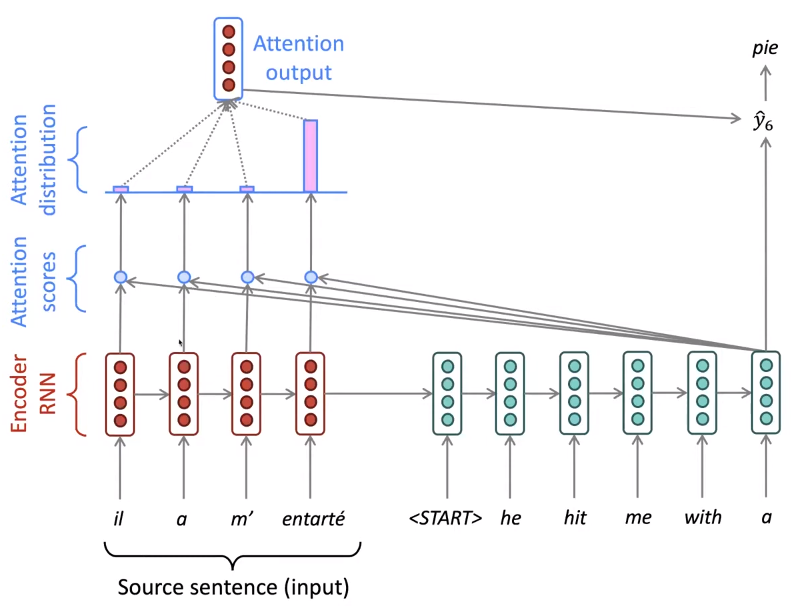
\includegraphics[scale=0.4]{img/seq2seq_attention.png}
    \end{center}
  \end{definition}

  Overall, attention is extremely useful in improving all performance, and it is intuitive with how humans analyze things, too. It significantly improves neural machine translation by allowing the decoder to focus on certain parts of the source. It also provides more ``human-like" model of the machine translation process (you can look back at the source sentence while translating, rather than needing to remember it all). It solves the bottleneck problem and helps with the vanishing gradient problem with these pseudo-residual connections through the context vector. 

  Finally, it provides some interpretability, as we can inspect the attention distribution to see what the decoder was focusing on (which again, we've never set explicitly but was learned by the model). 

  \begin{center}
    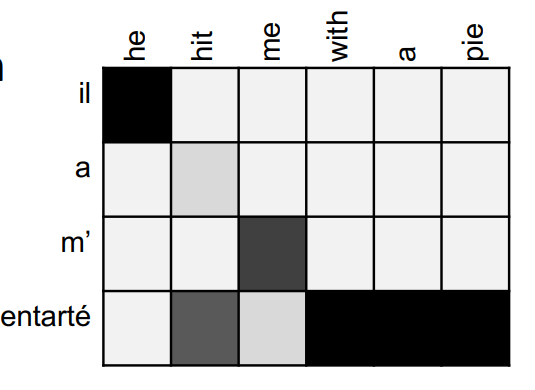
\includegraphics[scale=0.3]{img/attention_distribution.png}
  \end{center}

  \begin{code}
    For an implementation of this in PyTorch, look \href{code/seq2seq_attention.ipynb}{here}.
  \end{code}

  Now let's talk about how these parameters are already learned. The parameters of the model are. 
  \begin{enumerate}
    \item The encoding matrices for the usual seq2seq model: $\mathbf{W}_e, \mathbf{U}_e$. 
    \item Generating key, value, and query vectors for every possible embedding is not practical.\footnote{You would need three $d_{\mathrm{embedding}} \times |\mathcal{V}|$ matrices, where $\mathcal{V}$ is the set of our vocabulary, which can go easily past 500,000 elements.} A more compact way to represent them are through linear maps, so we are learning matrices $\mathbf{Q}, \mathbf{K}, \mathbf{V}$ such that 
    \begin{align*}
      \mathbf{q}_{t^\prime} & = \mathbf{Q} \mathbf{s}_{t^\prime} \\ 
      \mathbf{k}_t & = \mathbf{K} \mathbf{h}_t \\
      \mathbf{v}_t & = \mathbf{V} \mathbf{h}_t
    \end{align*}

    \item We should now have the decoding matrices $\mathbf{W}_d$ that takes in the attention context vector (plus maybe the previous hidden decoder state) and the original matrix $\mathbf{U}_d$. 
  \end{enumerate}
  Therefore, this problem reduces to learning the matrices $\mathbf{W}_e, \mathbf{U}_e, \mathbf{Q}, \mathbf{K}, \mathbf{V}, \mathbf{W}_d, \mathbf{U}_d$. 

  \begin{example}[Score Functions]
    Having additional flexibility with the score functions can also improve learning. We provide more examples here, which give more parameters to learn as well.  
    \begin{enumerate}
      \item The general attention model allows us to train a shared-weight matrix, allowing for $s \neq h$. 
      \[e^{t^\prime}_t = \mathrm{score}(\mathbf{s}_{t^\prime}, \mathbf{h}_t) = \mathbf{s}_{t^\prime}^T \mathbf{W}_a \mathbf{h}_t \in \mathbb{R}\]
      However, it may seem like there are too many parameters in $\mathbf{W}_a$, having to learn $sh$ values. 

      \item The reduced rank multiplicative attention uses low rank matrices, allowing us to learn only $ks + kh$ parameters for matrices $\mathbf{U}_a \in \mathbb{R}^{k \times s}, \mathbf{V}_a \in \mathbb{R}^{k \times h}$ where $k << s, h$. 
      \[e^{t^\prime}_t = \mathrm{score}(\mathbf{s}_{t^\prime}, \mathbf{h}_t) = \mathbf{s}_{t^\prime}^T (\mathbf{U}_a^T \mathbf{V}_a) \mathbf{h}_t = (\mathbf{U}_a \mathbf{s}_{t^\prime})^T (\mathbf{V}_a \mathbf{h}_t) \in \mathbb{R}\]

      \item Additive attention uses a neural net layer defined 
      \[e^{t^\prime}_t = \mathbf{v}_a^T \mathrm{tanh}(\mathbf{W}_a \mathbf{h}_t + \mathbf{V}_a \mathbf{s}_{t^\prime}) \in \mathbb{R}\]
      where $\mathbf{W}_a \in \mathbb{R}^{r \times h}, \mathbf{V}_a \in \mathbb{R}^{r \times s}$ are weight matrices, $\mathbf{v}_a \in \mathbb{R}^r$ is a weight vector, and $r$ (the attention dimensionality) is a hyperparameter. 
    \end{enumerate}
  \end{example}

  This can be naturally extended to other architectures, as we will explore later. 

  \begin{example}[Images]
    Given an image of size $224 \times 224$, we can make patches of size $16 \times 16$, and then flatten them to get a $196 \times 768$ matrix with a 2-dimensional positional encoding scheme. We can then apply a linear transformation to get the query, key, and value vectors.
  \end{example}

\subsection{Self-Attention Layer}

    While we have solved the bottleneck problem, this entire process is still sequential since every hidden decoder node requires us to know the previous hidden node. There are two sequential processes in the regular seq2seq attention model. 
    \begin{enumerate}
      \item The sequential encoding of the input sentence. 
      \item The sequential decoding of the output sentence. This unfortunately is not possible in transformers to parallelize. 
    \end{enumerate}

    We will focus on parallelizing the first part by temporarily forgetting about encoder-decoder models and just thinking about how to incorporate a good encoder with attention that is parallelizable. This extension is quite simple. Let $\mathbf{w}_{1:n}$ be a sequence of words in vocabulary $\mathcal{V}$. The key here is that rather than inputs having key-values and outputs having queries, \textit{all} words are associated with a 3-tuple of key, value, query. 
    \begin{equation}
      \mathbf{x}_i \mapsto (\mathbf{q}_i, \mathbf{k}_i, \mathbf{v}_i)
    \end{equation}

    \begin{definition}[Standard Scaled Dot-Product Attention]
      If we keep the score function to be the dot-product, the derivations become quite simple. 
      \begin{enumerate}
        \item For each $\mathbf{w}_i$, let $\mathbf{x}_i = E \mathbf{w}_i$ be the word embedding (with $E \in \mathbb{R}^{d \times |\mathcal{V}|}$ the embedding matrix). 

        \item We transform each word embedding with the (learned) weight matrices $\mathbf{Q}, \mathbf{K}, \mathbf{V}$. 
        \begin{align*} 
          \mathbf{q}_i & = \mathbf{Q} \mathbf{x}_i \implies Q = \mathbf{Q} X \\
          \mathbf{k}_i & = \mathbf{K} \mathbf{x}_i \implies K = \mathbf{K} X \\
          \mathbf{v}_i & = \mathbf{V} \mathbf{x}_i \implies V = \mathbf{V} X 
        \end{align*}
        where $X = [x_1, \ldots, x_n] \in \mathbb{R}^{d \times n}$.  

        \item We compute pairwise similarities between keys and queries and normalize with the softmax to get the attention distribution for each word. 
          \begin{equation}
            \mathbf{e}_{ij} = \mathbf{q}_i^T \mathbf{k}_j , \;\;\; \boldsymbol{\alpha}_{ij} = \frac{\exp(\mathbf{e}_{ij})}{\sum_{j^\prime} \exp(\mathbf{e}_{i j^\prime})}
          \end{equation}

        \item Compute the output for each word as a weighted sum of values. 
          \begin{equation}
            \mathbf{o}_i = \sum_j \boldsymbol{\alpha}_{ij} \mathbf{v}_j 
          \end{equation}
      \end{enumerate}

      Ultimately, this can be parallelized into one matrix operation.\footnote{Note that in order to even do such a thing, we must know $n$ beforehand. This can be solved by simply fixing some maximum length, padding everything to be some null token after the end token, and masking all the null tokens to be $0$. More on masking later. } 

      \begin{equation} 
        \mathrm{Attention}(Q, K, V) = \mathrm{softmax} \bigg( \frac{Q K^T}{\sqrt{E_k}} \bigg) V
      \end{equation}

      where the softmax is done to each row.\footnote{We divide by $\sqrt{E_k}$ to stabilize the gradients since as dimensionality increases, the dot product between random vectors tend to get large, leading to large softmax inputs. You can simply compute the variance of two $d$-dimensional Gaussian vectors and see that their variances scales linearly with $d$. }\footnote{You can see that if we have simple dot-product similarity scores, then $E_k = E_v$, but this need not be true in general. We will explore other similiarity score in the next subsection. } 

      Therefore, when you do a forward pass on an attention layer with input $x$, you first get the query vector $q$, extract the attention-weighted values from the key-value dictionary, and then return the weighted sum of the values. To give explicit parameterizations using the query, key, value encoding matrices, we can write this as 
      \begin{equation} 
        \mathrm{Attention}(x \,;\, \mathrm{Q}, \mathrm{K}, \mathrm{V}) = \mathrm{softmax} \bigg( \frac{(\mathbf{Q}x)(\mathbf{K} x)^T}{\sqrt{E_k}} \bigg) (\mathbf{V} x)
      \end{equation}

      This will give us a vector $\mathbf{o}_{1:n}$ consisting of the encoded vectors for each word in the sentence, and best of all, this is parallelizable! 
    \end{definition}

    There are three problems however. 
    \begin{enumerate}
      \item This self-attention encoding does not account for the position/order of the words. Therefore, some positional embedding is needed. 
      \item Our plan is to stack this layer multiple times on top of each other. However, we are just composing linear maps ultimately, so some nonlinearity is needed. 
      \item To use self-attention in \textit{decoders}, as we will see later on, we don't want to have any attention on later parts of a sentence, so we need some way to \textit{mask} future words. 
    \end{enumerate}

    We will deal with the first two problems and address the third problem in the transformer archictecture. 

  \subsubsection{Tokenization and Positional Embeddings}

    Given an input (or an output) $\mathbf{x}$, it must be tokenized into a sequence of tokens. This is a general preprocessing step that is done for any input, whether it be a sequence of words, a sequence of regions in an image, or a sequence of anything. The raw token data will be denoted $w_i$ for $i = 1, \ldots, n$.We can then embed these tokens into a vector space $x_i \in \mathbb{R}^d$. 

    As we will see later, attention does not have a way to discern the order of the input sequences. Therefore, we must add this positional information to the encoding. The most obvious way would be to simply concatenate the position of the token to the end with an index. 
    \begin{equation} 
      x_i \mapsto [x_i, i]
    \end{equation}
    However, this is not ideal since this tends to corrupt the embedding of the token. Instead, we can think of adding certain vectors representing components to the original embedding. 
    \begin{equation} 
      x_i \mapsto x_i + p_i
    \end{equation}
    Certain ways come to mind, such as simply letting $p_i$ be the vector of all $i$'s. This tends not to work in progress since the values of $i$ get too large and corrupts the embeddings too much.\footnote{A helpful Medium article \href{https://medium.com/@waelrashwan/demystifying-transformer-architecture-the-magic-of-positional-encoding-5fe8154d4a64}{here}} Normalizing the values of $i$ to be in $[0, 1]$ is disadvantageous because now the positional embedding $p_i$ is dependent on the length of the total input sequence. Therefore, we need two properties: 
    \begin{enumerate} 
      \item The positional encoding should be independent of the input sequence length. 
      \item The positional encoding shouldn't be too large that it corrupts the semantic meaning behind the original embedding. 
    \end{enumerate}
    It turns out that the sinusoidal function satisfies these properties. 

    \begin{definition}[Sinusoidal Position Embedding]
      Given the embeddings $x_i \in \mathbb{R}^{d}$, we can add a positional encoding to it by 
      \[x_i \mapsto x_i + p_i\]
      where the positional encoding is given by the vector where each component is defined as 
      \begin{equation} 
        (p_i)_j =  \begin{cases} 
            \sin \big( \frac{i}{10000^{2j/d}} \big) & \text{ if } j \text{ is even} \\ 
            \cos \big( \frac{i}{10000^{2j/d}} \big) & \text{ if } j \text{ is odd}
        \end{cases}
      \end{equation}
      where $i$ iterates through the tokens and $j$ iterates through the dimensions of the embedding. 
    \end{definition}

  \subsubsection{Stacked Attention Layers and Multi-Head Attention}

    The second problem of introducing nonlinearities is quite simple. Once we have the output of the first self-attention layer $\mathbf{o}_{1:n} = [\mathbf{o}_1, \ldots, \mathbf{o}_n]$, we can just input each $\mathbf{o}_i$ through a small MLP to introduce nonlinearity before inputting it into the next self-attention layer. 

    \begin{center}
      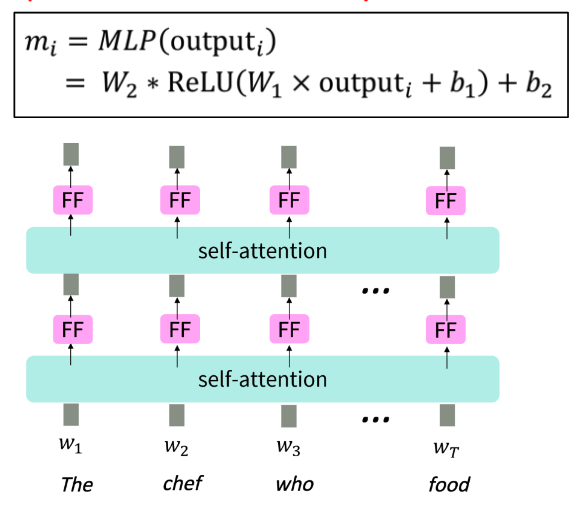
\includegraphics[scale=0.4]{img/stacked_self_attention_layers.png}
    \end{center}

    Boom, problem solved. 

    Going back, if we want to look at the attention for token $x_i$, we want to look through all $q_i^T k_j$ for all $j$ and find out where it is high. But perhaps we want to focus on different $j$ for different reasons. The following example may illustrate why. 

    \begin{example}[Semantic and Syntactic Attention]
      Given the sentence \textit{I went to the bank and got some money.}, one type of attention may look at the semantic meaning of the words, such as associating \textit{bank} with \textit{money}. However, we may also want to look at the syntactic meaning of the words, such as associating \textit{went} with \textit{bank}. When we read sentences, we have different types of attention for different reasons, and so having multiple heads of attention may be useful. 
    \end{example}

    \begin{definition}[Multi-Head Attention]
      Therefore, let us construct multiple attention heads by defining multiple triplets of $(Q, K, V)$ matrices. This may be more computationally inefficient, so we simply scale down the size of these matrices from 
      \[Q \in \mathbb{R}^{E_q \times d}, K \in \mathbb{R}^{E_k \times d}, V \in \mathbb{R}^{E_v \times d}\] 
      to 
      \[Q_\ell \in \mathbb{R}^{E_q \times d/h}, K_\ell \in \mathbb{R}^{E_k \times d/h}, V_\ell \in \mathbb{R}^{E_v \times d/h}\] 
      where $h$ is the number of heads. We are essentially decreasing the size of the token embedding dimension in order to get more heads. We can then do attention on each head separately. 
      \begin{equation} 
        \mathrm{Attention}_\ell = \mathrm{Attention}(Q_\ell, K_\ell, V_\ell) = \mathrm{softmax} \bigg( \frac{Q_\ell K_\ell^T}{\sqrt{E_k/h}} \bigg) V_\ell
      \end{equation}
      and we can simply concatenate them together to get the final output. 
      \[\mathrm{MultiHead}(Q, K, V) = \mathrm{Concat}(\mathrm{Attention}_1, \ldots, \mathrm{Attention}_h) W^O\]
      where $W^O \in \mathbb{R}^{d \times E_v}$ is a learnable weight matrix that mixes these heads together with a final linear transformation.\footnote{There is a valid concern that these heads may all end up learning the same thing and may just converge onto the same thing. However, this is not what happens in practice.} This entire process is shown in Figure \ref{fig:multi_head_attention}. 
    \end{definition}

    \begin{figure}[H]
      \centering 
      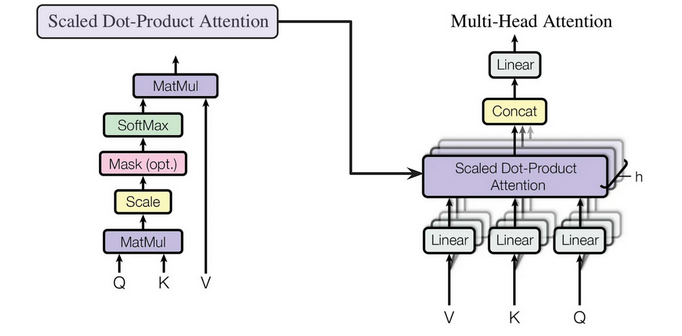
\includegraphics[scale=1.5]{img/multi_head_attention.png}
      \caption{Diagram of multi head attention. } 
      \label{fig:multi_head_attention}
    \end{figure}

\subsection{Transformers} 

    With self-attention out of the way, the transformer architecture becomes quite simple. An overview of it is shown in Figure \ref{fig:transformer}. 

    \begin{figure}[H]
      \centering 
      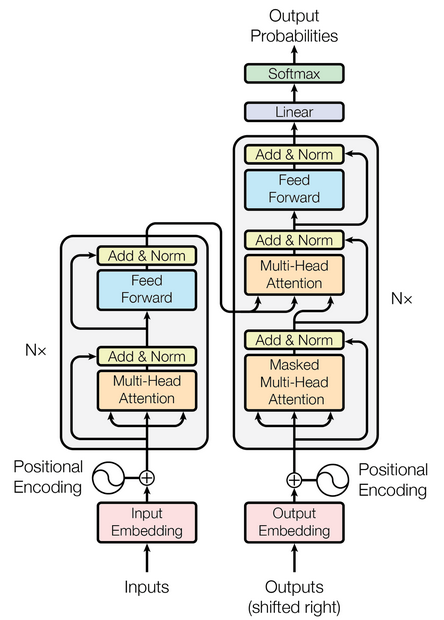
\includegraphics[scale=1.3]{img/transformer.png}
      \caption{Transformer architecture. } 
      \label{fig:transformer}
    \end{figure}

    The encoder is quite simple. You take the input embedding and add the positional embeddings to get $\{x_i \in \mathbb{R}^d\}_{i=1}^n$. You then pass it through a multi-head self-attention layer, which has outputs of shape $E_v \times n$, and then pass it through a feed forward network, adding residual connections and normalization layers to help with training. You then repeat this process $N$ times, which gives out the encoded sequence $\mathbf{h}_{1:n} = [\mathbf{h}_1, \ldots, \mathbf{h}_n]$, now ready to be fed into the decoder.\footnote{You can see that to support iterating through $n$ times, $E_v$ should equal $d$.}

    The decoder has two different self-attention layers. First, we run the generated output sequence through a masked self-attention layer, which generates the hidden nodes $\mathbf{z}_{1:n} = [\mathbf{z}_1, \ldots, \mathbf{z}_n]$ representing the state of the currently decoded sentence. Again, we have some maximum output length to ensure that we are working with a fixed size, and manually mask all tokens after the current one to be $0$.

    Then, another \textbf{cross-attention} layer takes both $\mathbf{h}_{1:n}$ and $\mathbf{z}_{1:n}$ and with its trained $(\mathbf{K}, \mathbf{V}, \mathbf{Q})$, computes the key, value, and query matrices as 
    \begin{equation}
      K = \mathbf{K} \mathbf{h}_{1:n}, \;\;\; V = \mathbf{V} \mathbf{h}_{1:n}, \;\;\; Q = \mathbf{Q} \mathbf{z}_{1:n}, 
    \end{equation}
    now ready to be plugged into to the self-attention formulas, integrating both the inputs and the current output to generate the result. This again outputs another list of vectors, which are run through an MLP and then have another set of $(\mathbf{K}, \mathbf{V}, \mathbf{Q})$ matrices waiting for them. This makes sense, since we want to use the output sequence to query the input key-values and attend to the correct set of tokens. 
    
    The output of this is then passed through a feed forward network, with some residual connections and normalization, and finally a linear layer transforms the output dimensions to whatever is needed (e.g. size of the vocabulary, or number of classes). Once this is done, a new word is generated,\footnote{Note that we have not specified how to get the corresponding word given an embedding vector. This is not within the scope of these notes and are covered in my natural language processing notes.} and this word (along with all previous words) is now used as the new input to the decoder in place of the start token. This process is done until the stop token is generated by the decoder. Notice that we encode with a bidirectional model (no masking) and generated the target with a unidirectional model (masking). 

    Note that again, parallelization of the decoder is not possible in the transformer architecture. Additionally, you can see that more normalization layers and residual connections are needed to train efficiently. This is very important in practice. 

    Despite all its advantages, self-attention has quadratic runtime complexity with respect to the sequence length since we need to compute attention for all pairs of words. This is worse than the linear runtime complexity in RNNs.  

  \subsubsection{Masking}

    The final aspect we did not address is the masking. When we are training the transformer on a corpus of data, the decoder first computes self-attention on all the previous outputs first to get the query, and then takes in the output of the encoder self-attention layer as the keys and values. Then it does self-attention once more over these triplets, essentially doing a self-attention layer over the entire input and all tokens up to the current decoded output. 

    When training this model, we have access to the entire decoded output, and we want to make sure that we do not perform self-attention on any future words since it will most likely attend 100\% to the next word to generate the next word! This does not learn anything, so we artificially set the attention distribution for all future output words to be $0$. This is usually done by setting the attention scores to $-\infty$ (or more practically, a very negative number) which will result in $0$ after softmaxing.\footnote{Here is a nice explanation \href{https://stackoverflow.com/questions/58127059/how-to-understand-masked-multi-head-attention-in-transformer}{here}.}

\subsection{Practical Implementation}

  In here we go over the nitty gritty details that comes into implementing a transformer in \texttt{pytorch==2.3.0}. 

  \subsubsection{Key, Value, Query Matrices and In Projections}

    The first thing is that these key, value, query does not have to necessarily equal to the dimension embedding, which we will denote as $E$. One flexibility is that we don't necessarily need to set the dimensions of the keys, values, and queries the same. We can see in the constructor of the \texttt{torch.nn.MultiheadAttention} module that you can input your own dimensions for the keys and values, but queries must be the same as $E$. 
    \begin{lstlisting}
      def __init__(self, embed_dim, num_heads, dropout=0., bias=True, add_bias_kv=False, add_zero_attn=False,
                   kdim=None, vdim=None, batch_first=False, device=None, dtype=None) -> None:
         ... 
        self.embed_dim = embed_dim
        self.kdim = kdim if kdim is not None else embed_dim
        self.vdim = vdim if vdim is not None else embed_dim
        self._qkv_same_embed_dim = self.kdim == embed_dim and self.vdim == embed_dim
    \end{lstlisting}

    In fact, $K \in \mathbb{R}^{d_k \times E}$, $V \in \mathbb{R}^{d_v \times E}$, then $QK^T \in \mathbb{R}^{E \times d_k}$. Since this obviously leads to dimension mismatch problem when we multiply it with the matrix $V$, what we do is have an \textbf{in projection} layer that maps everything to dimension $E$. We can check this for the following. 
    \begin{equation}
      K_{proj} \in \mathbb{R}^{E \times d_k}, V_{proj} \in \mathbb{R}^{E \times d_v}, Q_{proj} \in \mathbb{R}^{E \times E}
    \end{equation}
    There are two ways to store these projection matrices, as shown in the constructor. 
    \begin{lstlisting}
      # in the constructor 
      ...
      self._qkv_same_embed_dim = self.kdim == embed_dim and self.vdim == embed_dim

      if not self._qkv_same_embed_dim:
        self.q_proj_weight = Parameter(torch.empty((embed_dim, embed_dim), **factory_kwargs))
        self.k_proj_weight = Parameter(torch.empty((embed_dim, self.kdim), **factory_kwargs))
        self.v_proj_weight = Parameter(torch.empty((embed_dim, self.vdim), **factory_kwargs))
        self.register_parameter('in_proj_weight', None)
      else:
        self.in_proj_weight = Parameter(torch.empty((3 * embed_dim, embed_dim), **factory_kwargs))
        self.register_parameter('q_proj_weight', None)
        self.register_parameter('k_proj_weight', None)
        self.register_parameter('v_proj_weight', None)
    \end{lstlisting}
    \begin{enumerate}
      \item If these shapes are different, then we store them in separate matrices as above. 
      \begin{lstlisting}
        att = nn.MultiheadAttention(embed_dim=50, num_heads=1, bias=False, kdim=30, vdim=40) 
        att.q_proj_weight.shape # torch.Size([50, 50])
        att.k_proj_weight.shape # torch.Size([50, 30])
        att.v_proj_weight.shape # torch.Size([50, 40])
      \end{lstlisting}

      \item If these shapes are the same, then we just store them in a $3E \times E$ matrix by concatenation them. 
      \begin{lstlisting}
        att = nn.MultiheadAttention(embed_dim=50, num_heads=1, bias=False) 
        att.in_proj_weight.shape # torch.Size([150, 50])
      \end{lstlisting}
    \end{enumerate}
    These conditions are asserted throughout the forward pass as well.  

  \subsubsection{Masking} 

    We multiply by a masking matrix. 

  \subsubsection{Computing Attention}

    First we reshape them so that they are batch first. 

    If \texttt{needs\_weights = True}, we also output the attention weights in addition to the output, but it is said that this degrades performance. It is by default true but should be set to false for small tasks. 

  \subsubsection{Forward Pass of MultiheadAttention}

    First, we should look at the main function that computes self-attention. We omit a large part of the code to focus on the relevant details. 

    \begin{lstlisting}
      # torch.nn.functional 
      def multi_head_attention_forward(
        query: Tensor,
        key: Tensor,
        value: Tensor,
        embed_dim_to_check: int,
        num_heads: int,
        in_proj_weight: Optional[Tensor],
        in_proj_bias: Optional[Tensor],
        bias_k: Optional[Tensor],
        bias_v: Optional[Tensor],
        add_zero_attn: bool,
        dropout_p: float,
        out_proj_weight: Tensor,
        out_proj_bias: Optional[Tensor],
        training: bool = True,
        ...
      ): 
      # first unsqueezes the input if it is not batched. 

      # look at the input dimensions and check that multiheads divide it evenly 
      #  
      assert embed_dim == embed_dim_to_check, \
          f"was expecting embedding dimension of {embed_dim_to_check}, but got {embed_dim}"
      if isinstance(embed_dim, torch.Tensor):
          # embed_dim can be a tensor when JIT tracing
          head_dim = embed_dim.div(num_heads, rounding_mode='trunc')
      else:
          head_dim = embed_dim // num_heads
      assert head_dim * num_heads == embed_dim, f"embed_dim {embed_dim} not divisible by num_heads {num_heads}"
      if use_separate_proj_weight:
          # allow MHA to have different embedding dimensions when separate projection weights are used
          assert key.shape[:2] == value.shape[:2], \
              f"key's sequence and batch dims {key.shape[:2]} do not match value's {value.shape[:2]}"
      else:
          assert key.shape == value.shape, f"key shape {key.shape} does not match value shape {value.shape}"

      # Computes in-projection, which is an affine map before doing attention. 
      # in_proj_weight = [W_q, W_k, W_v], in_proj_bias = [b_q, b_k, b_v] 
      # computes q = q * W_q + b_q, k = k * W_k + b_k, v = v * W_v + b_v
      if not use_separate_proj_weight:
        q, k, v = _in_projection_packed(query, key, value, in_proj_weight, in_proj_bias)
      else:
        if in_proj_bias is None:
            b_q = b_k = b_v = None
        else:
            b_q, b_k, b_v = in_proj_bias.chunk(3)
        q, k, v = _in_projection(query, key, value, q_proj_weight, k_proj_weight, v_proj_weight, b_q, b_k, b_v)

      # prepare attention mask 
      # add bias along batch dimension  
      # more preparation with mask
      ... 
      # Now calculate attention
      if need_weights:
        # scale q_scale for the sqrt(E) division factor 
        B, Nt, E = q.shape
        q_scaled = q * math.sqrt(1.0 / float(E))

      if attn_mask is not None:
        # torch.baddbmm is a pybinded C function implementing matrix multiplication 
        # of form attn_mask + q_scaled @ k^T
        attn_output_weights = torch.baddbmm(attn_mask, q_scaled, k.transpose(-2, -1))
      else:
        # torch.bmm is also a pybinded C function q_scaled + k^T
        attn_output_weights = torch.bmm(q_scaled, k.transpose(-2, -1))
      ...
      # softmax it and then multiply it by V. 
      attn_output_weights = softmax(attn_output_weights, dim=-1)
      attn_output = torch.bmm(attn_output_weights, v)

      # final linear layer for more weightings. 
      attn_output = attn_output.transpose(0, 1).contiguous().view(tgt_len * bsz, embed_dim)
      attn_output = linear(attn_output, out_proj_weight, out_proj_bias)
      attn_output = attn_output.view(tgt_len, bsz, attn_output.size(1))

      # optionally average attention weights over heads
      attn_output_weights = attn_output_weights.view(bsz, num_heads, tgt_len, src_len)
      if average_attn_weights:
          attn_output_weights = attn_output_weights.mean(dim=1)

      if not is_batched:
          # squeeze the output if input was unbatched
          attn_output = attn_output.squeeze(1)
          attn_output_weights = attn_output_weights.squeeze(0)
      return attn_output, attn_output_weights
    \end{lstlisting}

    This is precisely the function that is called in the forward method of the \texttt{MultiheadAttention} module. 

  \subsubsection{Transformer}

    In the transformer, we can see that if we peek at the state dictionary, it composes of an encoder and a decoder, each with a certain number of attention layers. There are 6 attention layers each by default. 

    \begin{lstlisting}
      transformer = nn.Transformer()
      transformer.state_dict
      # output 
      <bound method Module.state_dict of Transformer(
        (encoder): TransformerEncoder(
          (layers): ModuleList(
            (0-5): 6 x TransformerEncoderLayer(
              (self_attn): MultiheadAttention(
                (out_proj): NonDynamicallyQuantizableLinear(in_feat
      ures=512, out_features=512, bias=True)
              )
              (linear1): Linear(in_features=512, out_features=2048,
       bias=True)
              (dropout): Dropout(p=0.1, inplace=False)
              (linear2): Linear(in_features=2048, out_features=512,
       bias=True)
              (norm1): LayerNorm((512,), eps=1e-05, elementwise_aff
      ine=True)
              (norm2): LayerNorm((512,), eps=1e-05, elementwise_aff
      ine=True)
              (dropout1): Dropout(p=0.1, inplace=False)
              (dropout2): Dropout(p=0.1, inplace=False)
            )
          )
          (norm): LayerNorm((512,), eps=1e-05, elementwise_affine=T
      rue)
        )
        (decoder): TransformerDecoder(
          (layers): ModuleList(
            (0-5): 6 x TransformerDecoderLayer(
              (self_attn): MultiheadAttention(
                (out_proj): NonDynamicallyQuantizableLinear(in_feat
      ures=512, out_features=512, bias=True)
              )
              (multihead_attn): MultiheadAttention(
                (out_proj): NonDynamicallyQuantizableLinear(in_feat
      ures=512, out_features=512, bias=True)
              )
              (linear1): Linear(in_features=512, out_features=2048,
       bias=True)
              (dropout): Dropout(p=0.1, inplace=False)
              (linear2): Linear(in_features=2048, out_features=512,
       bias=True)
              (norm1): LayerNorm((512,), eps=1e-05, elementwise_aff
      ine=True)
              (norm2): LayerNorm((512,), eps=1e-05, elementwise_aff
      ine=True)
              (norm3): LayerNorm((512,), eps=1e-05, elementwise_aff
      ine=True)
              (dropout1): Dropout(p=0.1, inplace=False)
              (dropout2): Dropout(p=0.1, inplace=False)
              (dropout3): Dropout(p=0.1, inplace=False)
            )
          )
          (norm): LayerNorm((512,), eps=1e-05, elementwise_affine=T
      rue)
        )
      )>
    \end{lstlisting}

\subsection{Vision Transformers} 

  We have hinted at attention being applicable in other architectures, and the most popular is in computer vision. Historically, CNNs were very useful because they take into account the locality and translational-invariance of objects in images inherently in the convolutions. This is a great strength of convolutional networks. 
  
  Can transformers beat this? These assumptions are not built into the architecture, and researchers were quite unsuccessful in passing the benchmarks set by CNNs, but it turned out that in 2020, with enough training and a large enough architecture, \textit{vision transformers} in fact did surpass CNNs. 

 
\section{Diffusion Models} 


 
\section{Bayesian Neural Networks} 

  Has no real application yet (except uncertainty quantification) so only in research. 

\section{Graph Neural Networks} 

Now we want to process data in a graph, which has no direct grid structure. The adjacency matrix may not be enough. For example, the molecular structure. Applications in recommender systems. 

The absolute value of the determinant of the cofactor expansion of a Laplacian matrix tells you the number of minimum spanning trees of the graph. 

Let $\mathcal{L} = \Delta$ with $\mathcal{L} u = \Delta u$. 
\begin{equation}
  \Delta u = \lambda u = \sum_{i=1}^n \frac{\partial u}{\partial x_i}
\end{equation}
for some $\lambda < 0$. The eigenvectors of $L$ are the fourier basis. This turns convolution into multiplication. 
\begin{equation}
  \frac{d^2 x}{d t^2} = - \lambda x 
\end{equation}


\section{Semi Supervised Learning} 

  There has been good stream of work done at Google Brain that first came up with MixMatch in 2019 \cite{berthelot2019mixmatch}, which combined the state of the art semi supervised methods. This model was then improved the next year with ReMixMatch \cite{berthelot2020remixmatch}, and then improved again with a much more simple model called FixMatch \cite{sohn2020fixmatch}. 

  \subsection{Pseudo Label Learning} 
    
    Generating psuedo labels on unlabeled datasets and training on them. 

  \subsection{Consistency Regularization}
    
    Ensuring that the model is consistent with its predictions on certain inputs and neighbors of the inputs. It relies on the assumption that perturbed versions of the same input should have the same output. When wanting to make sure that the outputs are consistent with augmentations of the input, this is called \textbf{augmentation anchoring}. There are ways in which we use a combination of \textbf{weak augmentation} and \textbf{strong augmentation} to achieve this. 

  \subsection{Distribution Alignment}

  \subsection{Weak Supervision} 

  \subsection{Student Teacher Models} 

 

\bibliographystyle{plain}
\bibliography{./bibfile}
\end{document}
